\documentclass[10pt]{book}

\usepackage{agri_style}

\begin{document}

% ==========================================================
% Front matter
% ==========================================================
\frontmatter

% --- Cover page ---
% ============================================================
% ปกหน้าตำราวิชาการมาตรฐานสากล (Academic Book Cover Architect)
% สไตล์เปิดโปร่ง ไร้กล่อง ไร้กรอบ พร้อมสัญลักษณ์ AI \& Deep Learning
% มหาวิทยาลัยราชภัฏรำไพพรรณี
% ============================================================
\thispagestyle{empty}
\begin{titlepage}
\begingroup
\setlength{\XeTeXlinebreakskip}{0pt}
\begin{tikzpicture}[remember picture, overlay]
    % 1. ภาพอาร์ตเวิร์ก 3D Pixar Semi-realistics แบบ Full-Bleed 100%
    \node[anchor=center, inner sep=0pt] at (current page.center) {
        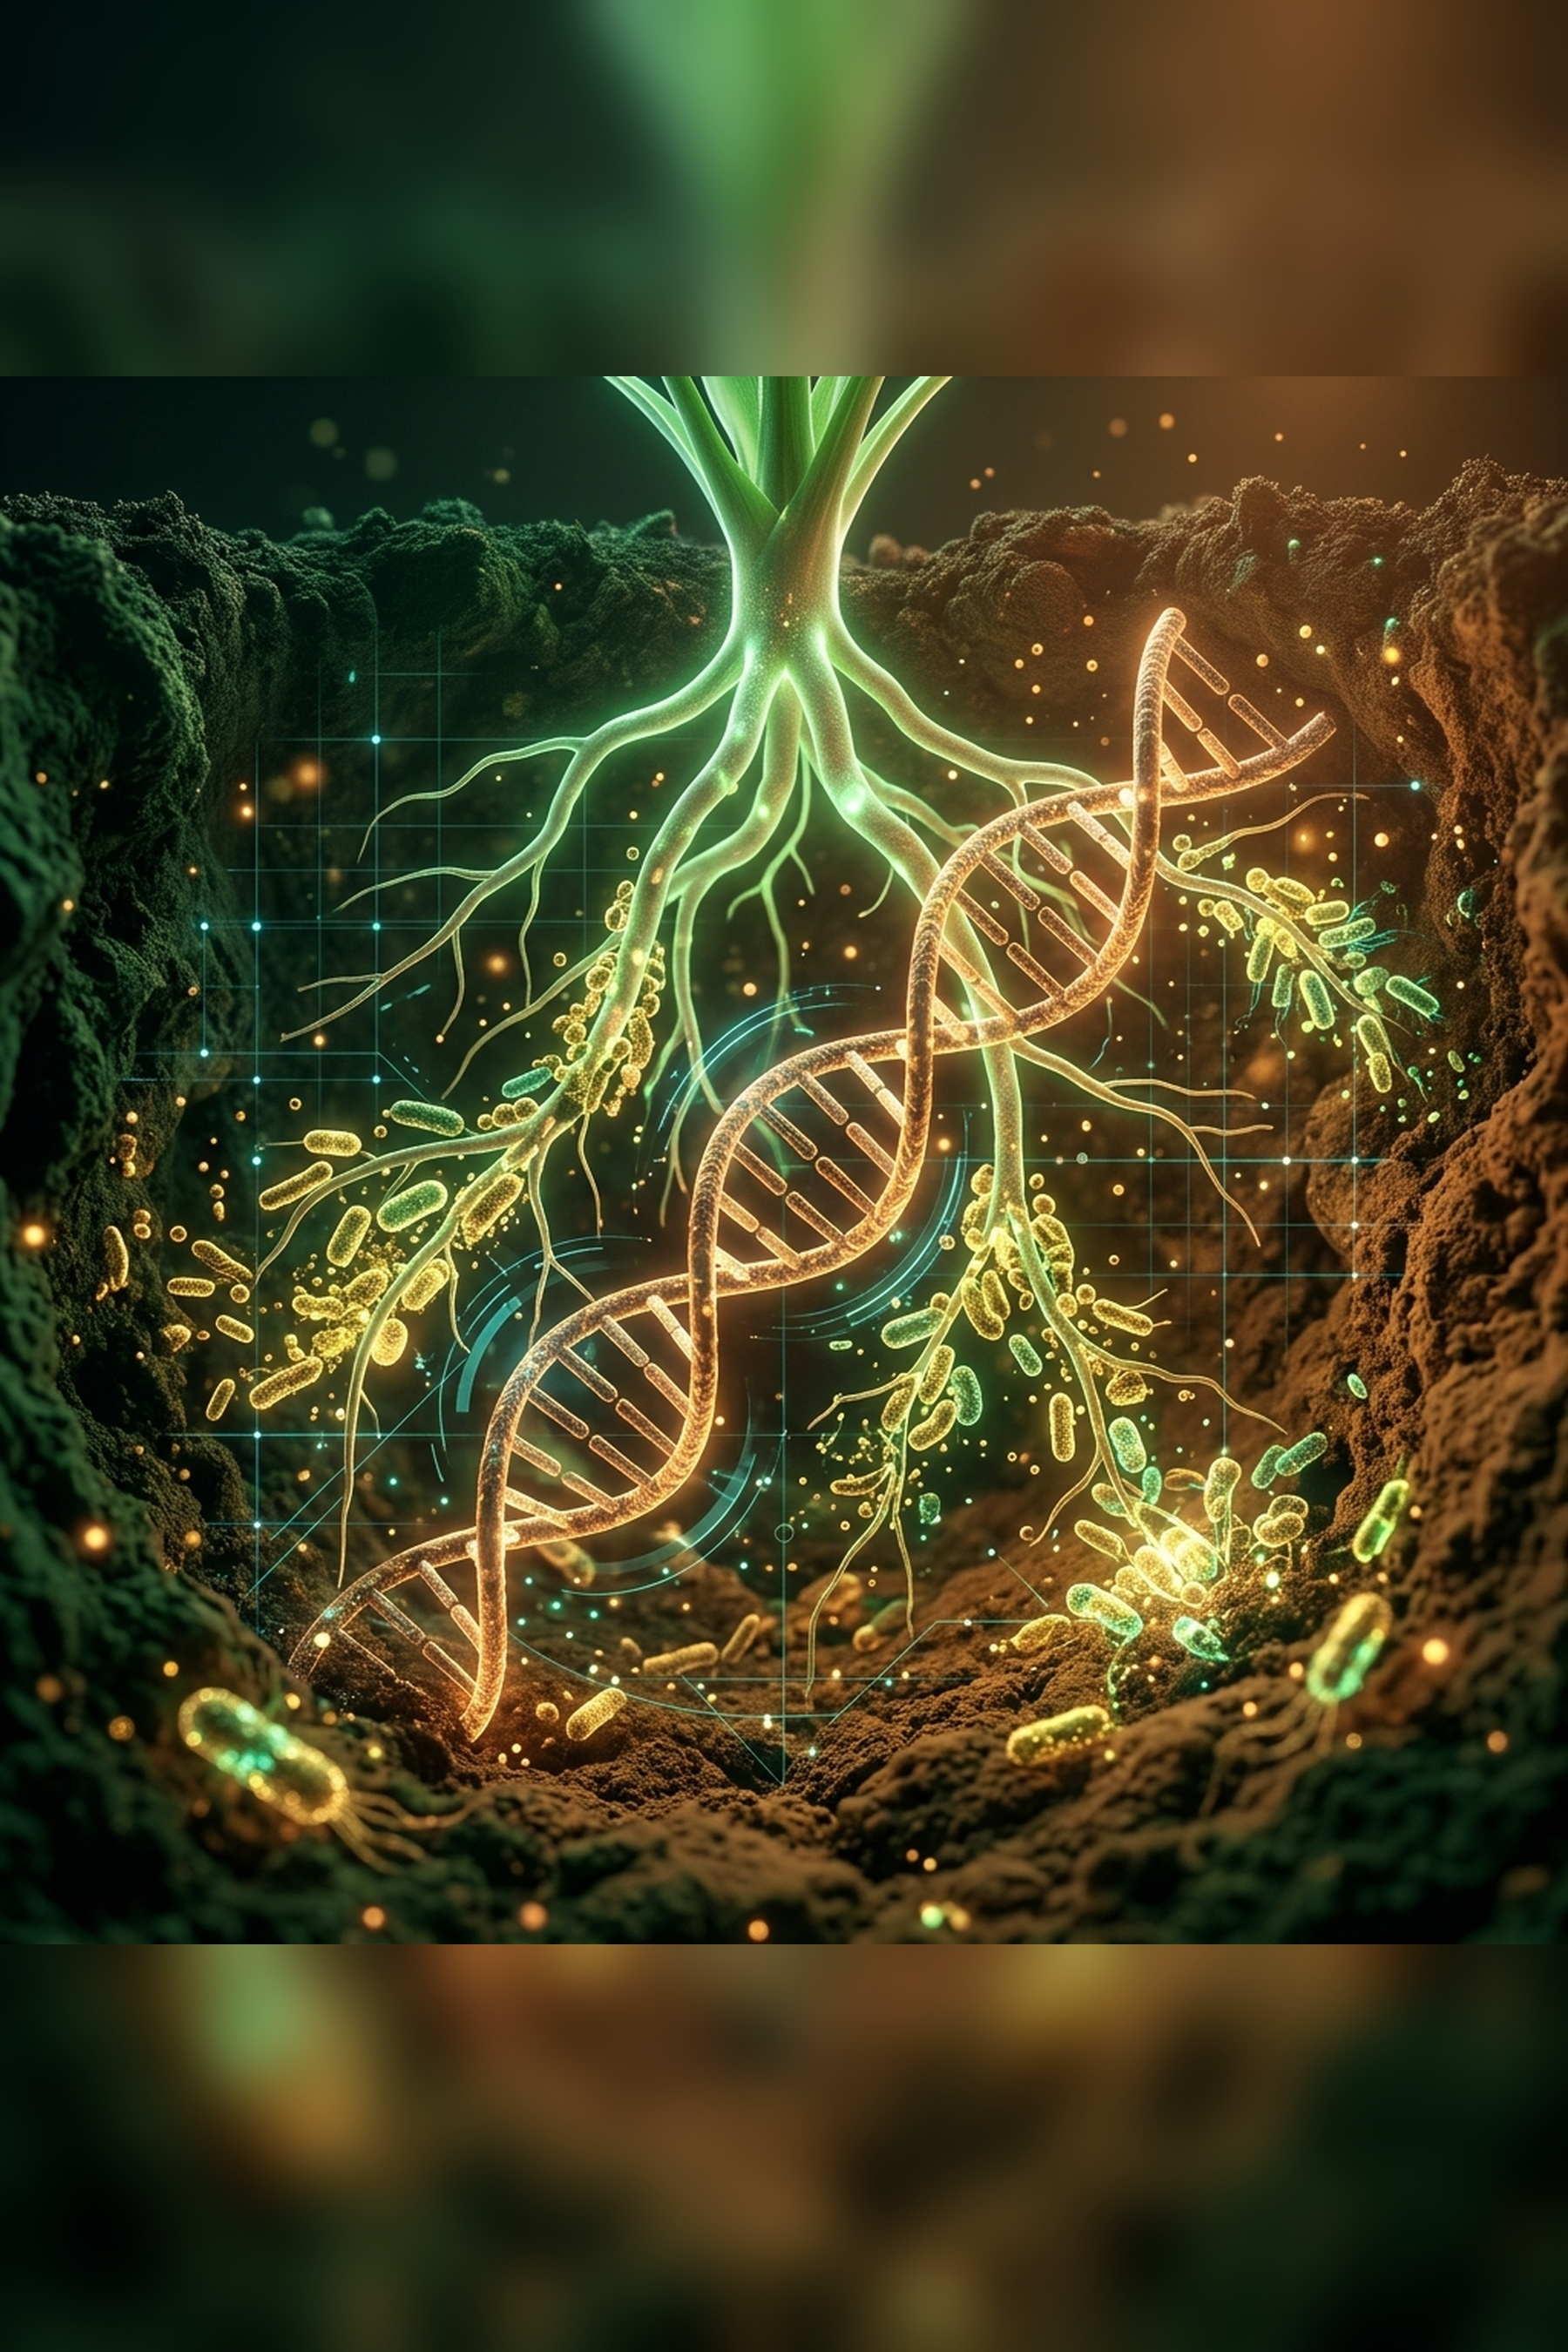
\includegraphics[width=\paperwidth, height=\paperheight]{assets/agri_cover_pixar_2x3.jpg}
    };

    % กำหนดสีสันสดใสระดับพรีเมียม (Curated Vibrant Palette)
    \definecolor{goldtitle}{RGB}{245, 195, 65}
    \definecolor{emeraldtitle}{RGB}{60, 230, 160}
    \definecolor{cyantitle}{RGB}{50, 220, 245}
    \definecolor{warmyellow}{RGB}{255, 235, 100}

    % ============================================================
    % สัญลักษณ์ AI / DEEP LEARNING (Header Neural Network Insignia)
    % ============================================================
    \begin{scope}[shift={([yshift=-0.60cm]current page.north)}]
        % Shadow layer
        \begin{scope}[shift={(0.6pt, -0.6pt)}]
            \foreach \ya in {-0.24, 0, 0.24} {
                \foreach \yb in {-0.34, -0.11, 0.11, 0.34} {
                    \draw[black!95, line width=0.5pt] (-2.2, \ya) -- (-1.8, \yb);
                }
            }
            \foreach \yb in {-0.34, -0.11, 0.11, 0.34} {
                \foreach \yc in {-0.17, 0.17} {
                    \draw[black!95, line width=0.5pt] (-1.8, \yb) -- (-1.4, \yc);
                }
            }
            \node[right, font=\fontsize{7pt}{8.5pt}\selectfont\bfseries, text=black!95] at (-1.25, 0) {ARTIFICIAL INTELLIGENCE \& DEEP LEARNING ARCHITECTURE};
        \end{scope}
        % Foreground layer
        \foreach \ya in {-0.24, 0, 0.24} {
            \foreach \yb in {-0.34, -0.11, 0.11, 0.34} {
                \draw[emeraldtitle!75, line width=0.4pt] (-2.2, \ya) -- (-1.8, \yb);
            }
        }
        \foreach \yb in {-0.34, -0.11, 0.11, 0.34} {
            \foreach \yc in {-0.17, 0.17} {
                \draw[goldtitle!75, line width=0.4pt] (-1.8, \yb) -- (-1.4, \yc);
            }
        }
        \foreach \ya in {-0.24, 0, 0.24} {
            \fill[emeraldtitle] (-2.2, \ya) circle (1.8pt);
            \draw[white, line width=0.3pt] (-2.2, \ya) circle (1.8pt);
        }
        \foreach \yb in {-0.34, -0.11, 0.11, 0.34} {
            \fill[emeraldtitle] (-1.8, \yb) circle (2pt);
            \draw[white, line width=0.3pt] (-1.8, \yb) circle (2pt);
        }
        \foreach \yc in {-0.17, 0.17} {
            \fill[goldtitle] (-1.4, \yc) circle (2.2pt);
            \draw[white, line width=0.3pt] (-1.4, \yc) circle (2.2pt);
        }
        \node[right, font=\fontsize{7pt}{8.5pt}\selectfont\bfseries, text=white] at (-1.25, 0) {ARTIFICIAL INTELLIGENCE \color{emeraldtitle}\&\ \color{goldtitle}DEEP LEARNING ARCHITECTURE};
    \end{scope}

    % ============================================================
    % 2. UPPER ZONE: ชื่อหนังสือแบบเปิด ไร้กล่อง ไร้กรอบ (Dual-Layer Micro Shadow)
    % ============================================================
    % เลเยอร์เงาคมชัด (Dark Drop Shadow Layer)
    \node[anchor=north, align=center, text width=14.0cm, inner sep=0pt] at ([xshift=0.6pt, yshift=-1.12cm]current page.north) {
        {\fontsize{8.5pt}{11pt}\selectfont\bfseries\color{black!95} AI-ENHANCED MICROBIO SERIES • เล่ม 2 • PRECISION AGRI-MICROBIOLOGY \& AIOT}\\[7pt]
        {\fontsize{24pt}{30pt}\selectfont\bfseries\color{black!98} จุลชีววิทยาการเกษตร และเทคโนโลยี AIoT}\\[7pt]
        {\fontsize{10.8pt}{15.5pt}\selectfont\bfseries\color{black!95} พลวัตของจุลินทรีย์ดิน ปุ๋ยชีวภาพ PGPR และการตรวจวินิจฉัยโรคพืชอัตโนมัติ}\\[6pt]
        {\fontsize{9pt}{12pt}\selectfont\bfseries\color{black!95} AGRICULTURAL MICROBIOLOGY AND AIOT SYSTEMS}
    };
    % เลเยอร์ตัวอักษรจริง สีสันสดใส คมชัดสูง (Foreground Vibrant Layer)
    \node[anchor=north, align=center, text width=14.0cm, inner sep=0pt] at ([yshift=-1.10cm]current page.north) {
        {\fontsize{8.5pt}{11pt}\selectfont\bfseries\color{emeraldtitle} AI-ENHANCED MICROBIO SERIES • เล่ม 2 • PRECISION AGRI-MICROBIOLOGY \& AIOT}\\[7pt]
        {\fontsize{24pt}{30pt}\selectfont\bfseries\color{white} จุลชีววิทยาการเกษตร\ \color{emeraldtitle}และเทคโนโลยี AIoT}\\[7pt]
        {\fontsize{10.8pt}{15.5pt}\selectfont\bfseries\color{warmyellow} พลวัตของจุลินทรีย์ดิน ปุ๋ยชีวภาพ PGPR และการตรวจวินิจฉัยโรคพืชอัตโนมัติ}\\[6pt]
        {\fontsize{9pt}{12pt}\selectfont\bfseries\color{white} AGRICULTURAL MICROBIOLOGY\ \color{goldtitle}AND AIOT SYSTEMS}
    };

    % ============================================================
    % 3. MIDGROUND: สัญลักษณ์ AI / Deep Learning HUD Reticle
    % ============================================================
    \begin{scope}[shift={([xshift=-3.2cm, yshift=1.2cm]current page.center)}]
        % Detection Bounding Box (Corner Brackets)
        \draw[emeraldtitle, line width=0.9pt] (-1.4,0.55) -- (-1.1,0.55);
        \draw[emeraldtitle, line width=0.9pt] (-1.4,0.55) -- (-1.4,0.25);
        \draw[emeraldtitle, line width=0.9pt] (1.4,0.55) -- (1.1,0.55);
        \draw[emeraldtitle, line width=0.9pt] (1.4,0.55) -- (1.4,0.25);
        \draw[emeraldtitle, line width=0.9pt] (-1.4,-0.55) -- (-1.1,-0.55);
        \draw[emeraldtitle, line width=0.9pt] (-1.4,-0.55) -- (-1.4,-0.25);
        \draw[emeraldtitle, line width=0.9pt] (1.4,-0.55) -- (1.1,-0.55);
        \draw[emeraldtitle, line width=0.9pt] (1.4,-0.55) -- (1.4,-0.25);
        % Subtle crosshair
        \draw[goldtitle!80, line width=0.5pt] (-0.2,0) -- (0.2,0);
        \draw[goldtitle!80, line width=0.5pt] (0,-0.2) -- (0,0.2);
        % HUD Label
        % Shadow layer
        \node[below, align=center, inner sep=0pt] at (0.5pt, -0.67) {
            {\fontsize{7pt}{8.5pt}\selectfont\bfseries\color{black!98} [ EDGE-AI [RandomForest/IoT] ]}\\[1.5pt]
            {\fontsize{6pt}{7.5pt}\selectfont\bfseries\color{black!98} PGPR Rhizosphere: \textbf{Optimal NPK}}
        };
        % Foreground layer
        \node[below, align=center, inner sep=0pt] at (0, -0.65) {
            {\fontsize{7pt}{8.5pt}\selectfont\bfseries\color{emeraldtitle} [ EDGE-AI [RandomForest/IoT] ]}\\[1.5pt]
            {\fontsize{6pt}{7.5pt}\selectfont\color{goldtitle} PGPR Rhizosphere: \textbf{Optimal NPK}}
        };
    \end{scope}

    % ============================================================
    % 4. LOWER ZONE: รายนามอาจารย์ผู้เขียน ไร้กล่อง ไร้กรอบ สลับชื่อตามประสงค์
    % ============================================================
    % เลเยอร์เงาล่าง (Drop Shadow Layer)
    \node[anchor=south, align=center, text width=14.0cm, inner sep=0pt] at ([xshift=0.6pt, yshift=0.88cm]current page.south) {
        {\fontsize{11.5pt}{15.5pt}\selectfont\bfseries\color{black!98} ผู้ช่วยศาสตราจารย์ ดร.จิรภัทร จันทมาลี \quad\textbullet\quad ผู้ช่วยศาสตราจารย์ ดร.ชีวะ ทัศนา}\\[3.5pt]
        {\fontsize{9.5pt}{13pt}\selectfont\bfseries\color{black!95} คณะวิทยาศาสตร์และเทคโนโลยี มหาวิทยาลัยราชภัฏรำไพพรรณี}\\[2.5pt]
        {\fontsize{8.5pt}{11pt}\selectfont\bfseries\color{black!95} ชุดตำรามาตรฐานวิชาการ AI-Enhanced MicroBio Series พ.ศ. 2569}
    };
    % เลเยอร์ตัวอักษรจริงล่าง (Foreground Layer)
    \node[anchor=south, align=center, text width=14.0cm, inner sep=0pt] at ([yshift=0.9cm]current page.south) {
        {\fontsize{11.5pt}{15.5pt}\selectfont\bfseries\color{white} ผู้ช่วยศาสตราจารย์ ดร.จิรภัทร จันทมาลี \quad{\color{goldtitle}\textbullet}\quad ผู้ช่วยศาสตราจารย์ ดร.ชีวะ ทัศนา}\\[3.5pt]
        {\fontsize{9.5pt}{13pt}\selectfont\bfseries\color{white!98} คณะวิทยาศาสตร์และเทคโนโลยี มหาวิทยาลัยราชภัฏรำไพพรรณี}\\[2.5pt]
        {\fontsize{8.5pt}{11pt}\selectfont\bfseries\color{goldtitle} ชุดตำรามาตรฐานวิชาการ AI-Enhanced MicroBio Series พ.ศ. 2569}
    };
\end{tikzpicture}
\endgroup
\end{titlepage}
\clearpage


% --- Copyright page ---
\newpage
\thispagestyle{empty}
\vspace*{\fill}

\begin{center}
\textbf{\large ข้อมูลทางบรรณานุกรมของสำนักหอสมุดแห่งชาติ}\\
\textbf{National Library of Thailand Cataloging in Publication Data}
\end{center}

\vspace{0.2cm}
\begin{tcolorbox}[colback=white, colframe=black, boxrule=0.8pt, arc=0pt, left=10pt, right=10pt, top=8pt, bottom=8pt]
\small
ชีวะ ทัศนา.\\
\hspace*{1.5em}\textbf{จุลชีววิทยาการเกษตรและเทคโนโลยี AIoT} = Agricultural microbiology and AIoT technology / ชีวะ ทัศนา และ จิรภัทร จันทมาลี. -- พิมพ์ครั้งที่ 1. -- จันทบุรี : คณะวิทยาศาสตร์และเทคโนโลยี มหาวิทยาลัยราชภัฏรำไพพรรณี, 2569.\\
\hspace*{1.5em}169 หน้า : ภาพประกอบ (บางภาพเป็นสี), แผนภูมิ, ตาราง ; 25 ซม. (มาตรฐาน B5)

\vspace{0.3cm}
\hspace*{1.5em}1. จุลชีววิทยาทางการเกษตร. 2. ปัญญาประดิษฐ์ทางการเกษตร. 3. อินเทอร์เน็ตของสรรพสิ่ง (IoT). 4. เกษตรกรรมแม่นยำ. I. จิรภัทร จันทมาลี, ผู้แต่งร่วม. II. ชื่อเรื่อง.

\vspace{0.3cm}
\noindent\textbf{QR51} \hfill \textbf{630.276}\\
\textbf{ISBN 978-616-94520-2-7 (e-book : PDF)}
\end{tcolorbox}

\vspace{0.4cm}
\noindent\textbf{จุลชีววิทยาการเกษตรและเทคโนโลยี AIoT}\\
\textbf{Agricultural Microbiology and AIoT Technology}

\vspace{0.2cm}
\noindent\textbf{ผู้เขียน:}\\
ผู้ช่วยศาสตราจารย์ ดร.ชีวะ ทัศนา\\
\textit{วท.บ. (ฟิสิกส์ประยุกต์), วท.ม. (ฟิสิกส์), ปร.ด. (ฟิสิกส์)}\\
ผู้ช่วยศาสตราจารย์ ดร.จิรภัทร จันทมาลี\\
\textit{วท.บ. (จุลชีววิทยา), วท.ม. (จุลชีววิทยาประยุกต์), ปร.ด. (เทคโนโลยีชีวภาพ)}

\vspace{0.2cm}
\noindent\textbf{สงวนลิขสิทธิ์ตามพระราชบัญญัติลิขสิทธิ์ พ.ศ. 2537 และที่แก้ไขเพิ่มเติม}\\
ห้ามลอกเลียนแบบ ดัดแปลง บันทึก หรือทำซ้ำส่วนใดส่วนหนึ่งของหนังสือเล่มนี้ ไม่ว่าด้วยกระบวนการทางอิเล็กทรอนิกส์ การถ่ายเอกสาร หรือวิธีการอื่นใด เว้นแต่จะได้รับอนุญาตเป็นลายลักษณ์อักษรจากคณะผู้เขียน เพื่อการศึกษาและวิจัยทางวิชาการที่ไม่แสวงหากำไร

\vspace{0.2cm}
\noindent\textbf{จัดพิมพ์และเผยแพร่โดย:}\\
คณะวิทยาศาสตร์และเทคโนโลยี มหาวิทยาลัยราชภัฏรำไพพรรณี\\
41 หมู่ 5 ตำบลท่าช้าง อำเภอเมือง จังหวัดจันทบุรี 22000\\
โทรศัพท์: 0-3931-9111 | เว็บไซต์: https://www.rbru.ac.th

\vspace{0.2cm}
\noindent\textbf{ข้อมูลการจัดพิมพ์:}\\
พิมพ์ครั้งที่ 1 (มิถุนายน พ.ศ. 2569)\\
รูปแบบสื่อ: E-Book (Interactive PDF, มาตรฐาน Academic B5 176 $\times$ 250 มม.)\\
จัดรูปเล่มด้วย: XeLaTeX \& TikZ Engine (TeX Live 2026)

% --- Preface ---
\chapter*{คำนำ}
\addcontentsline{toc}{chapter}{คำนำ}

หนังสือ \textbf{``จุลชีววิทยาการเกษตรและเทคโนโลยี AIoT''} เล่มนี้ ได้รับการพัฒนา ยกระดับ และขยายเนื้อหาอย่างลึกซึ้งตามมาตรฐานวิชาการระดับสากลและกรอบเกณฑ์มาตรฐาน ก.พ.อ. ระดับรองศาสตราจารย์ (รศ.) เพื่อให้สอดรับกับความก้าวหน้าอย่างก้าวกระโดดของวิทยาการคอมพิวเตอร์ชีวภาพ ปัญญาประดิษฐ์ (Artificial Intelligence) การเรียนรู้ของเครื่องและโครงข่ายประสาทเทียม (Machine Learning \& Deep Learning) ตลอดจนเทคโนโลยีชีวภาพสมัยใหม่ตามเกณฑ์มาตรฐานการศึกษา OBE (Outcome-Based Education)

เนื้อหาภายในเล่มได้รับการบูรณาการอย่างเป็นระบบครอบคลุม 11 บทเรียนและ 3 ภาคผนวก ตั้งแต่นิเวศวิทยาเชิงลึกของไรโซสเฟียร์และฟิลโลสเฟียร์ ชีวสรีรวิทยาของวัฏจักรสารอาหาร กลไกระดับโมเลกุลของแบคทีเรียส่งเสริมการเจริญเติบโตพืช (PGPR) และราไมคอร์ไรซา พยาธิกำเนิดของโรคพืชตามแบบจำลอง Zigzag Model และระบาดวิทยาเชิงปริมาณ ชีวเคมีของสารพิษ Bt และราปฏิปักษ์ วิศวกรรมการหมักปุ๋ยชีวภาพและการถ่ายโอนออกซิเจน ($k_L a$) จุลชีววิทยาในกระเพาะรูเมนและระบบไบโอฟล็อกในสัตว์น้ำ วิศวกรรมปุ๋ยหมักและแบบจำลอง Modified Gompertz ก๊าซชีวภาพ ตลอดจนการถอดรหัสพันธุกรรมเมตาเจโนมิกส์ (DADA2, QIIME2, SynComs) สถาปัตยกรรม AIoT และโทรมาตรแปลงเกษตร (RS485 Modbus RTU, LoRaWAN, Edge AI YOLOv8-Nano) พร้อมทั้งคู่มือปฏิบัติการทดลองมาตรฐาน 8 การทดลอง และภาคผนวกคลังสคริปต์ Python แผนผังวงจร และชุดคำสั่งพร้อมท์ AI อย่างครบครัน

คณะผู้เขียนหวังเป็นอย่างยิ่งว่า ตำราเล่มนี้จะเป็นแหล่งอ้างอิงทางวิชาการที่สำคัญ เป็นคู่มือในการพัฒนางานวิจัยขั้นสูง และสร้างแรงบันดาลใจให้แก่นักศึกษา นักวิจัย คณาจารย์ และนักวิชาการเกษตร ในการขับเคลื่อนภาคการเกษตรของไทยสู่อนาคตที่ยั่งยืน

\vspace{1cm}
\noindent\textbf{ผู้ช่วยศาสตราจารย์ ดร.ชีวะ ทัศนา\\ผู้ช่วยศาสตราจารย์ ดร.จิรภัทร จันทมาลี}\\
\textit{คณะวิทยาศาสตร์และเทคโนโลยี มหาวิทยาลัยราชภัฏรำไพพรรณี}\\
\textit{มิถุนายน 2569}

% --- Table of Contents ---
\tableofcontents

% --- List of Figures ---
\clearpage
\phantomsection
\addcontentsline{toc}{chapter}{\listfigurename}
\listoffigures

% --- List of Tables ---
\clearpage
\phantomsection
\addcontentsline{toc}{chapter}{\listtablename}
\listoftables

% ==========================================================
% Main matter
% ==========================================================
\mainmatter

\chapter{บทนำสู่จุลชีววิทยาการเกษตร}
\label{ch:intro}

\begin{keyconcept}[แนวคิดสำคัญของบทที่ 1]
จุลชีววิทยาการเกษตร\index{จุลชีววิทยาการเกษตร (Agricultural Microbiology)} (Agricultural Microbiology) เป็นศาสตร์บูรณาการที่ศึกษาบทบาท ความหลากหลาย และกิจกรรมทางชีวเคมีของประชากรจุลินทรีย์ในระบบนิเวศเกษตรกรรม ทั้งในดิน น้ำ พืช สัตว์ และผลผลิตหลังการเก็บเกี่ยว จุลินทรีย์ทำหน้าที่เป็นตัวขับเคลื่อนหลักในวัฏจักรชีวธรณีเคมี การตรึงธาตุอาหาร การควบคุมศัตรูพืชโดยชีววิธี และการสร้างความสมบูรณ์ของโครงสร้างดิน การนำเทคโนโลยีสารสนเทศ การวิเคราะห์ข้อมูลขนาดใหญ่ และปัญญาประดิษฐ์\index{ปัญญาประดิษฐ์ทางการเกษตร (Agri-AI)} (AI) เข้ามาผสานกับองค์ความรู้ด้านไมโครไบโอมดิน\index{ไมโครไบโอมดิน (Soil Microbiome)} กำลังเปลี่ยนผ่านระบบเกษตรกรรมแบบดั้งเดิมสู่เกษตรกรรมแม่นยำสูง (Precision Agriculture) และความมั่นคงทางอาหารอย่างยั่งยืน
\end{keyconcept}

\begin{figure}[ht]
    \centering
    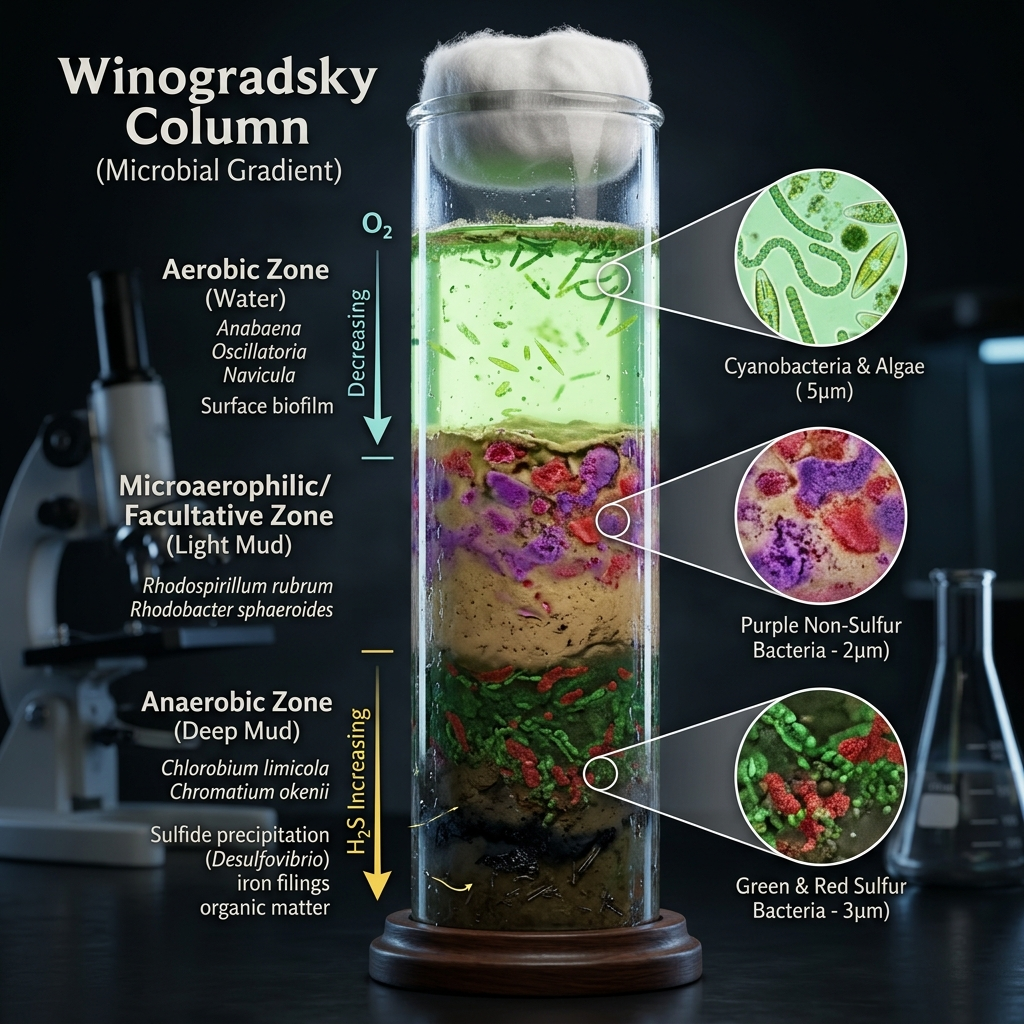
\includegraphics[width=0.85\textwidth]{assets/ch01_winogradsky_column.png}
    \caption{แบบจำลองสามมิติของ Winogradsky Column แสดงการจำแนกชั้นจุลินทรีย์ตามความลาดชันของความเข้มข้นออกซิเจนและไฮโดรเจนซัลไฟด์ ตั้งแต่ชั้นออกซิเจนสูงด้านบนจนถึงชั้นไร้ออกซิเจนที่มีการสะสมซัลไฟด์เข้มข้นด้านล่าง}
    \label{fig:ch01_winogradsky}
\end{figure}

\section*{วัตถุประสงค์การเรียนรู้ประจำบท}
เมื่อศึกษาบทเรียนนี้จบแล้ว นักศึกษาสามารถ:
\begin{enumerate}
    \item อธิบายขอบเขต ความหมาย และปฏิสัมพันธ์หลักของจุลินทรีย์ในระบบนิเวศการเกษตรได้อย่างถูกต้อง
    \item สรุปวิวัฒนาการทางประวัติศาสตร์ การค้นพบครั้งสำคัญ และคุณูปการของนักบุกเบิกจุลชีววิทยาการเกษตร
    \item วิเคราะห์การแบ่งชั้นทางชีวเคมีและสมดุลรีดอกซ์ในแบบจำลองคอลัมน์วิโนกราดสกี (Winogradsky Column)
    \item คำนวณอัตราการเติบโตจำเพาะของจุลินทรีย์ในดินด้วยแบบจำลองจลนศาสตร์ของโมโนด์ (Monod Kinetics)
    \item ประเมินความสำคัญของไมโครไบโอมต่อการขับเคลื่อนเกษตรกรรมยั่งยืนและการฟื้นฟูดินในยุคดิจิทัล
\end{enumerate}

\section{ขอบเขตและความสำคัญของจุลชีววิทยาการเกษตร}

จุลชีววิทยาการเกษตรเป็นสหวิทยาการขั้นสูงที่เชื่อมประสานองค์ความรู้จากวิทยาศาสตร์ดิน (Soil Science) สรีรวิทยาของพืช (Plant Physiology) ชีวเคมี พันธุศาสตร์ระดับโมเลกุล และวิทยาการคำนวณ เพื่อทำความเข้าใจบทบาทของจุลินทรีย์ในมิติต่าง ๆ โดยจำแนกออกเป็น 4 ขอบข่ายหลักได้แก่:

\begin{enumerate}
    \item \textbf{จุลชีววิทยาดิน (Soil Microbiology):} ศึกษาความหลากหลาย ชุมชน และกิจกรรมทางเมแทบอลิซึมของจุลินทรีย์ดินที่มีผลต่อการย่อยสลายอินทรียวัตถุและการหมุนเวียนธาตุอาหาร
    \item \textbf{จุลชีววิทยาปฏิสัมพันธ์ระหว่างพืชกับจุลินทรีย์ (Plant-Microbe Interactions):} ศึกษาความสัมพันธ์ทั้งในรูปแบบส่งเสริมการเจริญเติบโต (Plant Growth-Promoting Microorganisms: PGPM) และการเข้าทำลายของเชื้อก่อโรคพืช (Phytopathogens)
    \item \textbf{เทคโนโลยีชีวภาพปุ๋ยชีวภาพและชีวภัณฑ์ (Biofertilizers and Biocontrol Biotechnology):} การคัดเลือก การเพาะเลี้ยงในถังปฏิกรณ์ชีวภาพ และการผลิตหัวเชื้อจุลินทรีย์เชิงพาณิชย์เพื่อทดแทนเคมีเกษตร
    \item \textbf{จุลชีววิทยาหลังการเก็บเกี่ยวและผลพลอยได้ทางการเกษตร (Post-harvest and Agro-waste Microbiology):} การป้องกันการเน่าเสียของผลผลิต และการแปรสภาพของเสียทางการเกษตรให้เป็นปุ๋ยหมักและพลังงานชีวภาพ
\end{enumerate}

\begin{table}[ht]
\centering
\small
\begin{tabular}{lp{4.2cm}p{4.2cm}}
\toprule
\textbf{มิติทางเกษตรกรรม} & \textbf{กลไกการทำงานของจุลินทรีย์} & \textbf{ผลลัพธ์ต่อความยั่งยืน} \\
\midrule
การหมุนเวียนธาตุอาหาร & ตรึงไนโตรเจน, ละลายฟอสเฟตและโพแทสเซียม, ออกซิไดซ์กำมะถัน & ลดการพึ่งพาปุ๋ยเคมีสังเคราะห์ ลดการชะล้างไนเตรตลงสู่แหล่งน้ำ \\
การปรับปรุงสุขภาพดิน & สังเคราะห์สารเมือกพอลิแซ็กคาไรด์และเส้นใยราสร้างเม็ดดิน (Aggregates) & เพิ่มการอุ้มน้ำ ถ่ายเทอากาศดี และป้องกันการชะล้างพังทลายของหน้าดิน \\
การควบคุมโรคและศัตรูพืช & แย่งชิงพื้นที่ สร้างสารปฏิชีวนะ ย่อยผนังเซลล์ และกระตุ้นภูมิคุ้มกันพืช (ISR) & ลดสารเคมีฆ่าแมลงและยาฆ่าราตกค้างในห่วงโซ่อาหาร \\
การบำบัดฟื้นฟูดิน & ย่อยสลายสารกำจัดวัชพืชตกค้างและเปลี่ยนรูปโลหะหนัก (Bioremediation) & คืนความอุดมสมบูรณ์และลดความเป็นพิษในพื้นที่เกษตรปนเปื้อน \\
\bottomrule
\end{tabular}
\caption{บทบาทหน้าที่สำคัญของจุลินทรีย์ในการขับเคลื่อนระบบนิเวศเกษตรกรรมยั่งยืน}
\label{tab:ch01_roles}
\end{table}

\subsection{ปฏิสัมพันธ์ระหว่างจุลินทรีย์กับสิ่งมีชีวิตในระบบเกษตรกรรม}

ในแปลงเกษตรกรรม จุลินทรีย์ไม่ได้ดำรงชีวิตอยู่อย่างโดดเดี่ยว แต่สร้างเครือข่ายความสัมพันธ์อันซับซ้อนในระดับประชากรและชุมชน:

\begin{itemize}
    \item \textbf{ภาวะพึ่งพากัน (Mutualism):\index{ภาวะพึ่งพากัน (Mutualism)}} สิ่งมีชีวิตทั้งสองฝ่ายได้ประโยชน์ร่วมกันอย่างแนบแน่น หากขาดฝ่ายใดฝ่ายหนึ่งจะไม่สามารถดำรงชีวิตได้อย่างสมบูรณ์ เช่น แบคทีเรีย \organism{Rhizobium}\index{Rhizobium@\textit{Rhizobium}} ในปมรากพืชตระกูลถั่ว หรือเชื้อราอาร์บัสคูลาร์ไมคอร์ไรซา (AMF)\index{Arbuscular Mycorrhizal Fungi (AMF)} ที่ช่วยดูดฟอสฟอรัสแลกกับคาร์โบไฮเดรตจากพืช
    \item \textbf{ภาวะเกื้อกูลหรืออิงอาศัย (Commensalism):\index{ภาวะเกื้อกูล (Commensalism)}} ฝ่ายหนึ่งได้ประโยชน์โดยที่อีกฝ่ายหนึ่งไม่ได้และไม่เสียประโยชน์ เช่น แบคทีเรียเอพิไฟต์ (Epiphytic bacteria) บนผิวใบและผิวรากที่ใช้สารคัดหลั่งจากพืชเป็นแหล่งอาหาร
    \item \textbf{ภาวะปฏิปักษ์และการแข่งขัน (Antagonism and Competition):\index{ภาวะปฏิปักษ์ (Antagonism)}} การขัดขวางหรือยับยั้งการเจริญเติบโตของจุลินทรีย์อื่นเพื่อแย่งชิงพื้นที่และสารอาหาร เช่น เชื้อรา \organism{Trichoderma}\index{Trichoderma@\textit{Trichoderma}} หลั่งเอนไซม์ทำลายเส้นใยเชื้อราก่อโรค
    \item \textbf{ภาวะปรสิตและการก่อโรค (Parasitism and Pathogenicity):\index{ภาวะปรสิต (Parasitism)}} จุลินทรีย์เข้าไปอยู่อาศัยและดึงสารอาหารจากพืชเจ้าบ้านจนทำให้เกิดอาการผิดปกติ เช่น เชื้อรา \organism{Phytophthora palmivora}\index{Phytophthora palmivora@\textit{Phytophthora palmivora}} ก่อโรครากเน่าโคนเน่า หรือแบคทีเรีย \organism{Ralstonia solanacearum}\index{Ralstonia solanacearum@\textit{Ralstonia solanacearum}} ก่อโรคเหี่ยวเขียว
\end{itemize}

\section{วิวัฒนาการทางประวัติศาสตร์และผู้บุกเบิกจุลชีววิทยาการเกษตร}

การทำความเข้าใจบทบาทของจุลินทรีย์ในดินใช้เวลาสั่งสมองค์ความรู้ยาวนานกว่าสองศตวรรษ โดยผ่านการเปลี่ยนผ่านกระบวนทัศน์ (Paradigm Shifts) สำคัญ:

\subsection{ยุคบุกเบิกและการค้นพบการสังเคราะห์ทางเคมี (ศตวรรษที่ 19)}

\begin{itemize}
    \item \textbf{Jean-Baptiste Boussingault (1838):} นักเคมีเกษตรชาวฝรั่งเศส เป็นผู้ริเริ่มทำการทดลองเชิงปริมาณเพื่อศึกษาความสมดุลของไนโตรเจนในการหมุนเวียนพืช และพิสูจน์ว่าพืชตระกูลถั่วสามารถเพิ่มปริมาณไนโตรเจนในแปลงปลูกได้
    \item \textbf{Hermann Hellriegel และ Hermann Wilfarth (1888):} ค้นพบหลักฐานชี้ชัดว่าความสามารถในการตรึงไนโตรเจนของพืชตระกูลถั่วเกิดขึ้นจากความสัมพันธ์แบบพึ่งพากับแบคทีเรียที่อาศัยอยู่ในปมราก ไม่ใช่ความสามารถของเนื้อเยื่อพืชโดยลำพัง
    \item \textbf{Sergei Winogradsky (1856--1953):\index{Winogradsky, Sergei}} นักจุลชีววิทยาชาวรัสเซีย ผู้ได้รับการยกย่องเป็น "บิดาแห่งจุลชีววิทยาสิ่งแวดล้อมและจุลชีววิทยาดิน" ค้นพบกระบวนการ \textbf{Chemolithotrophy\index{Chemolithotrophy}} ซึ่งพิสูจน์ว่าจุลินทรีย์สามารถดำรงชีวิตและสังเคราะห์สารอินทรีย์โดยใช้พลังงานจากการออกซิไดซ์สารอนินทรีย์ เช่น แอมโมเนีย ไนไตรต์ หรือไฮโดรเจนซัลไฟด์ นอกจากนี้ยังสามารถแยกเชื้อแบคทีเรียตรึงไนโตรเจนอิสระแบบไม่ใช้ออกซิเจน \organism{Clostridium pasteurianum}\index{Clostridium pasteurianum@\textit{Clostridium pasteurianum}} ได้สำเร็จ
    \item \textbf{Martinus Beijerinck (1851--1931):\index{Beijerinck, Martinus}} นักจุลชีววิทยาชาวดัตช์ ผู้คิดค้นเทคนิคการเพาะเลี้ยงแบบคัดเลือก (Enrichment Culture Technique\index{Enrichment culture}) ซึ่งเปิดประตูสู่การแยกจุลินทรีย์ที่มีหน้าที่เฉพาะทาง และสามารถแยกเชื้อแบคทีเรียตรึงไนโตรเจนในปมรากถั่ว \organism{Rhizobium leguminosarum}\index{Rhizobium leguminosarum@\textit{Rhizobium leguminosarum}} และแบคทีเรียตรึงไนโตรเจนอิสระแบบใช้ออกซิเจน \organism{Azotobacter chroococcum}\index{Azotobacter chroococcum@\textit{Azotobacter chroococcum}}
\end{itemize}

\subsection{ยุคปฏิวัติเขียวสู่ยุคอณูชีววิทยาและ AIoT สมัยใหม่}

ในช่วงกลางศตวรรษที่ 20 นวัตกรรมการสังเคราะห์แอมโมเนียด้วยกระบวนการทางเคมี Haber-Bosch นำไปสู่การใช้ปุ๋ยไนโตรเจนสังเคราะห์และการปฏิวัติเขียว (Green Revolution) ผลิตผลทางการเกษตรเพิ่มขึ้นอย่างก้าวกระโดด แต่สร้างผลกระทบข้างเคียงรุนแรงต่อความหลากหลายทางชีวภาพของดินและสมดุลนิเวศ

เข้าสู่ศตวรรษที่ 21 การกำเนิดของเทคโนโลยี Next-Generation Sequencing (NGS) และเมตาเจโนมิกส์ (Metagenomics) ทำให้นักวิทยาศาสตร์สามารถเข้าถึงข้อมูลพันธุกรรมของจุลินทรีย์ในดินกว่า 99\% ที่ไม่สามารถเพาะเลี้ยงในห้องปฏิบัติการได้ (Unculturable Microorganisms) ร่วมกับการนำเทคโนโลยีโทรมาตร IoT และโมเดลปัญญาประดิษฐ์ (AI) เข้ามาตรวจวัดและทำนายพฤติกรรมของชุมชนจุลินทรีย์แบบเรียลไทม์

\section{แบบจำลองคอลัมน์วิโนกราดสกี (Winogradsky Column) และพลวัตทางเคมี}

คอลัมน์วิโนกราดสกี\index{Winogradsky Column} เป็นระบบนิเวศจำลองขนาดเล็ก (Microcosm) ที่แสดงให้เห็นการหมุนเวียนธาตุอาหารและการพึ่งพาอาศัยกันของจุลินทรีย์ต่างกลุ่มตามความลาดชันของออกซิเจน แสง และซัลเฟอร์

\begin{figure}[ht]
\centering
\begin{tikzpicture}[scale=0.9, >=Stealth]
    % Tube outline
    \draw[thick, fill=blue!8] (0,0) rectangle (4,8);
    
    % Zones
    \fill[agriGreen!25] (0,6.2) rectangle (4,8);
    \node at (2,7.1) [align=center] {\footnotesize \textbf{Aerobic Zone ($O_2$ สูง, $H_2S$ ต่ำ)}\\Algae, Cyanobacteria};
    
    \fill[mbAmber!20] (0,4.2) rectangle (4,6.2);
    \node at (2,5.2) [align=center] {\footnotesize \textbf{Microaerophilic Zone}\\Purple Non-Sulfur Bacteria};
    
    \fill[purple!20] (0,2.0) rectangle (4,4.2);
    \node at (2,3.1) [align=center] {\footnotesize \textbf{Anaerobic Zone (แสงส่องถึง)}\\Purple \& Green Sulfur Bacteria};
    
    \fill[black!30] (0,0) rectangle (4,2.0);
    \node at (2,1.0) [align=center] {\footnotesize \textbf{Deep Anaerobic Zone ($H_2S$ สูง)}\\Cellulose Degraders, SRB};
    
    % Arrows for gradients
    \draw[->, very thick, color=red!70!black] (-0.6,1) -- (-0.6,7) node[midway, left, align=center]{\small ออกซิเจน ($O_2$)};
    \draw[->, very thick, color=agriGreen!80!black] (4.6,7) -- (4.6,1) node[midway, right, align=center]{\small ไฮโดรเจนซัลไฟด์ ($H_2S$)};
\end{tikzpicture}
\caption{แผนภาพแสดงความลาดชันทางเคมีชีวภาพและการจำแนกโซนจุลินทรีย์ใน Winogradsky Column}
\label{fig:winogradsky_diagram}
\end{figure}

\begin{table}[ht]
\centering
\small
\begin{tabular}{lp{3.5cm}p{4.5cm}}
\toprule
\textbf{ชั้นความลึก} & \textbf{กลุ่มจุลินทรีย์เด่น} & \textbf{ปฏิกิริยาเมแทบอลิซึมหลัก} \\
\midrule
โซนบน (Aerobic) & ไซยาโนแบคทีเรีย, สาหร่ายสีเขียว & สังเคราะห์แสงใช้น้ำ ปลดปล่อย $O_2$ ($2H_2O \rightarrow O_2 + 4H^+ + 4e^-$) \\
โซนกลาง (Microaerophilic) & \organism{Rhodospirillum}, \organism{Rhodobacter} & สังเคราะห์แสงแบบไม่ใช้ออกซิเจน ใช้สารอินทรีย์เป็นตัวให้อิเล็กตรอน \\
โซนล่าง (Anaerobic แสงถึง) & \organism{Chromatium} (ราสีม่วง), \organism{Chlorobium} (ราสีเขียว) & สังเคราะห์แสงโดยใช้ $H_2S$ เป็นตัวให้อิเล็กตรอน ($CO_2 + 2H_2S \xrightarrow{\text{light}} (CH_2O) + 2S^0 + H_2O$) \\
โซนก้นขวด (Deep Anaerobic) & \organism{Desulfovibrio}, \organism{Clostridium} & รีดิวซ์ซัลเฟตสร้างก๊าซไข่เน่า ($SO_4^{2-} \rightarrow H_2S$) และย่อยสลายเซลลูโลส \\
\bottomrule
\end{tabular}
\caption{รายละเอียดเมแทบอลิซึมของจุลินทรีย์ในแต่ละชั้นของคอลัมน์วิโนกราดสกี}
\label{tab:winogradsky_metabolism}
\end{table}

\section{จลนศาสตร์การเจริญเติบโตของจุลินทรีย์ในดิน (Soil Microbial Growth Kinetics)}

การทำความเข้าใจพลวัตของประชากรจุลินทรีย์ในดินภายใต้สารอาหารที่มีจำกัด จำเป็นต้องอาศัยแบบจำลองทางคณิตศาสตร์ โดยแบบจำลองพื้นฐานที่เป็นรากฐานสำคัญคือ \textbf{แบบจำลองโมโนด์ (Monod Equation)\index{แบบจำลองโมโนด์ (Monod Model)}\index{จลนศาสตร์การเจริญ (Growth Kinetics)}}:

\begin{equation}
\mu = \mu_{\max} \frac{S}{K_s + S}
\label{eq:monod}
\end{equation}

เมื่อ:
\begin{itemize}
    \item $\mu$ คือ อัตราการเจริญเติบโตจำเพาะ (Specific Growth Rate)\index{อัตราการเติบโตจำเพาะ ($\mu$)} มีหน่วยเป็น $\text{h}^{-1}$ หรือ $\text{day}^{-1}$
    \item $\mu_{\max}$ คือ อัตราการเจริญเติบโตจำเพาะสูงสุด (Maximum Specific Growth Rate)\index{อัตราการเติบโตจำเพาะสูงสุด ($\mu_{\max}$)}
    \item $S$ คือ ความเข้มข้นของสารอาหารที่จำกัดการเจริญเติบโต (Limiting Substrate Concentration) ($\text{mg/L}$ หรือ $\text{g/kg}$ ดิน)
    \item $K_s$ คือ ค่าคงที่กึ่งอิ่มตัวของสารอาหาร (Substrate Constant หรือ Affinity Constant)\index{ค่าคงที่กึ่งอิ่มตัว ($K_s$)}
\end{itemize}
\begin{itemize}
    \item $\mu$ คือ อัตราการเจริญเติบโตจำเพาะของจุลินทรีย์ (Specific Growth Rate, $\text{hr}^{-1}$ หรือ $\text{day}^{-1}$)
    \item $\mu_{\max}$ คือ อัตราการเจริญเติบโตจำเพาะสูงสุดภายใต้สารอาหารล้นเกิน ($\text{hr}^{-1}$)
    \item $S$ คือ ความเข้มข้นของสารอาหารที่เป็นปัจจัยจำกัด (Substrate Concentration, mg/L หรือ mg/kg)
    \item $K_s$ คือ ค่าคงที่กึ่งอิ่มตัวของสารอาหาร (Half-velocity Constant) ซึ่งมีค่าเท่ากับความเข้มข้นสารอาหาร ณ จุดที่ $\mu = 0.5 \mu_{\max}$
\end{itemize}

ในกรณีที่สารอาหารหรือสารปนเปื้อนมีความเข้มข้นสูงเกินไปจนเกิดการยับยั้งการเจริญเติบโต (Substrate Inhibition) เช่น ความเข้มข้นของแอมโมเนียหรือสารประกอบฟีนอล จะใช้ **แบบจำลองฮัลเดน (Haldane Kinetics)**:

\begin{equation}
\mu = \mu_{\max} \frac{S}{K_s + S + \frac{S^2}{K_i}}
\label{eq:haldane}
\end{equation}
โดยที่ $K_i$ คือ ค่าคงที่ของการยับยั้งจากสารตั้งต้น (Inhibition Constant)

\begin{worked}[ตัวอย่างที่ 1.1 การคำนวณอัตราการเจริญเติบโตจำเพาะของแบคทีเรียย่อยอินทรียวัตถุในดิน]
แบคทีเรีย \organism{Bacillus subtilis} ในดินแปลงปลูกทุเรียน มีอัตราการเจริญเติบโตสูงสุด $\mu_{\max} = 0.45\text{ hr}^{-1}$ และมีค่าสัมพรรคภาพต่อกลูโคสในสารคัดหลั่งรากพืช $K_s = 15\text{ mg/L}$ 
จงคำนวณอัตราการเจริญเติบโตจำเพาะ ($\mu$) ใน 2 กรณีต่อไปนี้:
\begin{enumerate}
    \item บริเวณดินห่างจากรากพืชที่มีความเข้มข้นกลูโคสเจือจางเพียง $S_1 = 5\text{ mg/L}$
    \item บริเวณผิวสัมผัสรากพืช (Rhizoplane) ที่มีสารคัดหลั่งเข้มข้น $S_2 = 60\text{ mg/L}$
\end{enumerate}

\textbf{วิธีทำ:}
1. กรณีดินห่างราก ($S_1 = 5\text{ mg/L}$):
$$\mu_1 = 0.45 \times \frac{5}{15 + 5} = 0.45 \times \frac{5}{20} = 0.1125\text{ hr}^{-1}$$
2. กรณีผิวสัมผัสราก ($S_2 = 60\text{ mg/L}$):
$$\mu_2 = 0.45 \times \frac{60}{15 + 60} = 0.45 \times \frac{60}{75} = 0.3600\text{ hr}^{-1}$$

\textbf{บทวิเคราะห์ผลลัพธ์:} อัตราการเจริญเติบโตของแบคทีเรียบริเวณผิวรากสูงกว่าบริเวณดินรอบนอกถึง $3.2$ เท่า แสดงให้เห็นว่าสารคัดหลั่งรากพืชมีบทบาทขับเคลื่อนประชากรจุลินทรีย์อย่างมีนัยสำคัญ ส่งผลให้เกิดปรากฏการณ์ไรโซสเฟียร์ (Rhizosphere Effect)
\end{worked}

% [RESEARCH-UPDATE-2026-10]
\section{ความก้าวหน้างานวิจัยล่าสุดด้านจุลชีววิทยาเกษตรยั่งยืน}

งานวิจัยระดับนานาชาติในช่วงปี ค.ศ. 2024–2026 ได้ชี้ให้เห็นทิศทางใหม่ของการผสานวิทยาการด้าน Culturomics ร่วมกับเมตาเจโนมิกส์ความละเอียดสูง \cite{pmid39526137} ซึ่งช่วยให้นักวิจัยสามารถแยกจุลินทรีย์สายพันธุ์หายากที่เคยเชื่อว่าเพาะเลี้ยงไม่ได้ นำมาศึกษาคุณสมบัติทางพันธุศาสตร์และการเป็นชีวภัณฑ์

นอกจากนี้ การทบทวนปฏิสัมพันธ์ระหว่างพืช ดิน และไมโครไบโอมแบบสามเส้า (Tripartite Plant-Soil-Microbiome Interactions) \cite{pmid41800415} ชี้ชัดว่าสุขภาพของพืชไม่ได้ขึ้นอยู่กับธาตุอาหารทางเคมีเพียงอย่างเดียว แต่ถูกกำหนดโดยความหลากหลายเชิงหน้าที่ (Functional Redundancy) ของกลุ่มจุลินทรีย์ประจำถิ่น ซึ่งช่วยให้พืชรอดพ้นจากสภาวะอากาศสุดขั้วอันเนื่องมาจากโลกรวน (Climate Change)

\begin{insight}[ประเด็นวิเคราะห์เชิงวิชาการ]
หากความหลากหลายของจุลินทรีย์ดินลดลงเนื่องจากการไถพรวนและการใช้สารเคมีต่อเนื่องยาวนาน ระบบเกษตรกรรมจะสูญเสียความสามารถในการฟื้นตัว (Ecosystem Resilience) นักคิดว่าการนำระบบเซนเซอร์วัดค่าชีวภาพของดินร่วมกับ AI สามารถช่วยกำหนดแผนการฟื้นฟูจุลินทรีย์เฉพาะพื้นที่ได้อย่างไร?
\end{insight}

\section*{สรุปประจำบท}

จุลชีววิทยาการเกษตรเป็นรากฐานของความมั่นคงทางอาหารและระบบเกษตรกรรมยั่งยืน การศึกษาความสัมพันธ์ระหว่างพืช ดิน และจุลินทรีย์ที่เริ่มต้นจากผลงานบุกเบิกของ Winogradsky และ Beijerinck ได้พัฒนาสู่การจำลองจลนศาสตร์และอณูชีววิทยาระดับสูง แบบจำลองคอลัมน์วิโนกราดสกีและสมการโมโนด์แสดงให้เห็นว่ากิจกรรมของจุลินทรีย์ถูกขับเคลื่อนด้วยพลังงานเคมีชีวภาพและข้อจำกัดของสารตั้งต้น การทำความเข้าใจกลไกเหล่านี้ทำให้สามารถออกแบบสูตรปุ๋ยชีวภาพและมาตรการควบคุมศัตรูพืชได้อย่างแม่นยำ

\subsection*{คำถามท้ายบทและการวิเคราะห์}

\noindent \textbf{ระดับที่ 1: ความรู้และความเข้าใจเชิงทฤษฎี (Knowledge \& Comprehension)}
\begin{enumerate}
    \item อธิบายขอบเขตของ "จุลชีววิทยาการเกษตร" และเปรียบเทียบความแตกต่างด้านเป้าหมายการศึกษากับ "จุลชีววิทยาทางการแพทย์"
    \item Sergei Winogradsky ค้นพบกระบวนการ Chemolithotrophy อย่างไร และกระบวนการนี้มีความสำคัญต่อการหมุนเวียนธาตุอาหารในดินอย่างไร?
    \item การค้นพบของ Hermann Hellriegel และ Hermann Wilfarth ในปี 1888 ได้เปลี่ยนกระบวนทัศน์เรื่องการตรึงไนโตรเจนอย่างไร?
    \item วิเคราะห์การแบ่งชั้นใน Winogradsky Column เหตุใดแบคทีเรียกลุ่ม Purple sulfur bacteria จึงเจริญอยู่ใต้ชั้นของ Purple non-sulfur bacteria?
\end{enumerate}

\noindent \textbf{ระดับที่ 2: การวิเคราะห์และการคำนวณเชิงปริมาณ (Quantitative Analysis \& Calculation)}
\begin{enumerate}[resume]
    \item ในสมการจลนศาสตร์ของโมโนด์ ค่าคงที่กึ่งอิ่มตัว ($K_s$) สะท้อนคุณสมบัติทางสรีรวิทยาใดของจุลินทรีย์ และหากจุลินทรีย์ A มีค่า $K_s$ ต่ำกว่าจุลินทรีย์ B จะมีความได้เปรียบอย่างไรในสภาพดินขาดแคลนสารอาหาร?
    \item หากแบคทีเรียดินชนิดหนึ่งมี $\mu_{\max} = 0.5\text{ day}^{-1}$, $K_s = 20\text{ mg/kg}$ จงคำนวณหาความเข้มข้นของสารอาหาร $S$ ที่ทำให้อัตราการเจริญเติบโตมีค่าเท่ากับ $0.4\text{ day}^{-1}$
    \item อธิบายความแตกต่างระหว่างแบบจำลองจลนศาสตร์ของ Monod และ Haldane พร้อมยกตัวอย่างสารในแปลงเกษตรที่อาจทำให้เกิดปรากฏการณ์ Substrate Inhibition
\end{enumerate}

\noindent \textbf{ระดับที่ 3: การสังเคราะห์และการแก้ปัญหาในแปลงจริง (Application \& Real-World Synthesis)}
\begin{enumerate}[resume]
    \item เปรียบเทียบผลกระทบของการปฏิวัติเขียว (Green Revolution) ที่มีต่อผลผลิตพืชในระยะสั้นกับความหลากหลายของจุลินทรีย์ดินในระยะยาว
    \item ปรากฏการณ์ "Rhizosphere Effect" มีสาเหตุจากปัจจัยใด และพืชใช้กลไกใดในการคัดเลือกประชากรจุลินทรีย์ที่เป็นประโยชน์มารอบราก?
    \item จากงานวิจัยล่าสุดด้าน Tripartite Interactions ปัจจัยการเปลี่ยนแปลงสภาพภูมิอากาศส่งผลกระทบต่อกิจกรรมของจุลินทรีย์ดินอย่างไรบ้าง และนักวิจัยจะนำ AIoT มาช่วยฟื้นฟูระบบนิเวศดินเฉพาะพื้นที่ได้อย่างไร?
\end{enumerate}

\chapter{จุลินทรีย์ในดินและวัฏจักรชีวธรณีเคมี}
\label{ch:soil_microbes}

\begin{keyconcept}[แนวคิดสำคัญของบทที่ 2]
ดินไม่ได้เป็นเพียงสสารทางกายภาพสำหรับการค้ำจุนต้นพืช แต่เป็นระบบนิเวศทางชีวภาพที่มีความหลากหลายสูงที่สุดแห่งหนึ่งบนโลก จุลินทรีย์ดิน (Soil Microorganisms)\index{จุลินทรีย์ดิน (Soil Microorganisms)} ทำหน้าที่เป็นโรงงานเคมีชีวภาพที่ขับเคลื่อนวัฏจักรชีวธรณีเคมี (Biogeochemical Cycles)\index{วัฏจักรชีวธรณีเคมี (Biogeochemical Cycles)} หลัก ได้แก่ วัฏจักรคาร์บอน ไนโตรเจน ฟอสฟอรัส และซัลเฟอร์ การเปลี่ยนรูปทางเคมีเหล่านี้กำหนดความพร้อมของธาตุอาหารที่พืชสามารถดูดซึมไปใช้ การสร้างอินทรียวัตถุในดิน และการกักเก็บคาร์บอนในระยะยาว (Soil Carbon Sequestration)\index{การกักเก็บคาร์บอนในดิน (Soil Carbon Sequestration)} ซึ่งเป็นหัวใจสำคัญของการฟื้นฟูความอุดมสมบูรณ์ของดินและการเกษตรที่ทนทานต่อสภาพภูมิอากาศ
\end{keyconcept}

\begin{figure}[ht]
    \centering
    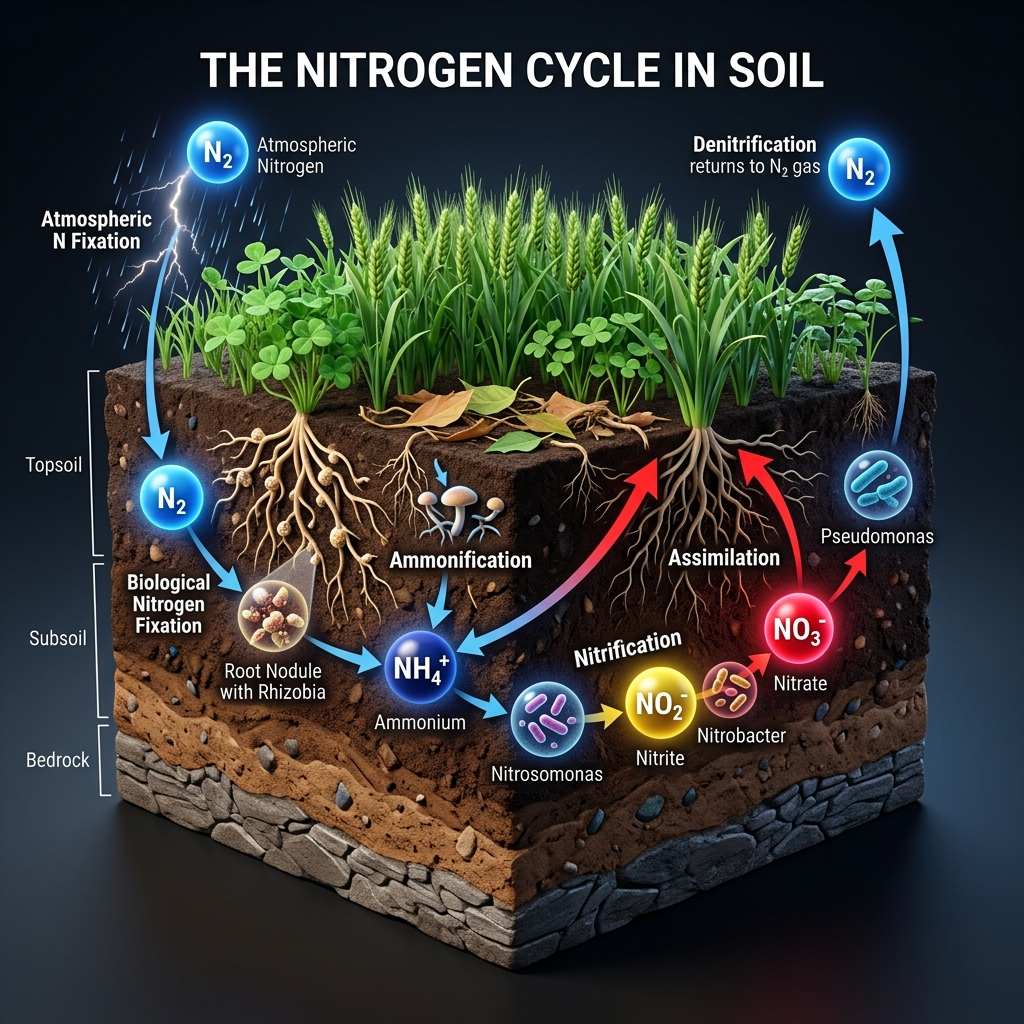
\includegraphics[width=0.85\textwidth]{assets/ch02_nitrogen_cycle.png}
    \caption{แผนภาพ 3D แสดงวัฏจักรไนโตรเจนในดินและเครือข่ายการทำงานร่วมกันของจุลินทรีย์ ตั้งแต่การตรึงไนโตรเจนทางชีวภาพ กระบวนการไนตริฟิเคชันโดยแบคทีเรียและอาร์เคีย ไปจนถึงกระบวนการดีไนตริฟิเคชันในสภาวะไร้ออกซิเจน}
    \label{fig:ch02_nitrogen_cycle}
\end{figure}

\section*{วัตถุประสงค์การเรียนรู้ประจำบท}
เมื่อศึกษาบทเรียนนี้จบแล้ว นักศึกษาสามารถ:
\begin{enumerate}
    \item จำแนกคุณลักษณะทางกายภาพ เคมี และชีวภาพของดินที่เป็นตัวกำหนดถิ่นที่อยู่อาศัยของจุลินทรีย์
    \item อธิบายกลไกการย่อยสลายสารอินทรีย์และทฤษฎีปั๊มคาร์บอนของจุลินทรีย์ (Microbial Carbon Pump) ในวัฏจักรคาร์บอน
    \item วิเคราะห์ขั้นตอนเคมีชีวภาพและสมการสมดุลในวัฏจักรไนโตรเจน (BNF, Nitrification, Denitrification, Anammox)
    \item อธิบายกลไกการละลายฟอสฟอรัสและวัฏจักรซัลเฟอร์ในดินกรดและดินน้ำขัง
    \item คำนวณสมดุลการตรึงไนโตรเจนและการเปลี่ยนแปลงอัตราส่วน C:N ต่อกระบวนการ Mineralization และ Immobilization
\end{enumerate}

\section{ดินในฐานะแหล่งที่อยู่อาศัยของจุลินทรีย์ (Soil as a Microbial Habitat)}

ดินเป็นระบบสามเฟสที่ประกอบด้วยเฟสของแข็ง (แร่ธาตุอนินทรีย์ 45\% และอินทรียวัตถุ 5\%) เฟสของเหลว (สารละลายดิน 25\%) และเฟสก๊าซ (อากาศในดิน 25\%) โครงสร้างเม็ดดิน (Soil Aggregates) ถูกจำแนกออกเป็นเม็ดดินขนาดใหญ่ (Macroaggregates, $>250\,\mu\text{m}$) และเม็ดดินขนาดเล็ก (Microaggregates, $<250\,\mu\text{m}$) 

ภายในเม็ดดินเหล่านี้มีช่องว่างระหว่างอนุภาค (Pore Network) ซึ่งสร้างไมโครแฮบิแทต (Microhabitats) ที่หลากหลาย จุลินทรีย์ดินส่วนใหญ่อาศัยอยู่รวมกันเป็นแผ่นฟิล์มชีวภาพ (Biofilms) เกาะติดกับผิวแร่ดินเหนียวและสารฮิวมัส โดยมีปัจจัยทางสิ่งแวดล้อมควบคุมกิจกรรมดังนี้:

\begin{itemize}
    \item \textbf{ความเป็นกรด-ด่างของดิน (Soil pH):} เป็นปัจจัยหลักที่กำหนดองค์ประกอบชุมชนจุลินทรีย์ ในดินกรด ($\text{pH} < 5.5$) เชื้อราจะมีความได้เปรียบในการเจริญเติบโตเนื่องจากทนกรดได้ดี ขณะที่แบคทีเรียส่วนใหญ่ชอบสภาวะเป็นกลางถึงด่างอ่อน ($\text{pH } 6.5$--$7.5$)
    \item \textbf{ศักย์รีดอกซ์ (Redox Potential, $E_h$):} บ่งชี้สถานะการถ่ายโอนอิเล็กตรอนในดิน ดินที่มีการถ่ายเทอากาศดีจะมีค่า $E_h > +400\text{ mV}$ (สภาวะใช้ออกซิเจน) ในขณะที่ดินน้ำขัง เช่น นาข้าว จะมีค่า $E_h$ ลดลงต่ำกว่า $-100\text{ mV}$ ทำให้เกิดสภาวะไม่ใช้ออกซิเจน
    \item \textbf{ศักย์ของน้ำในดิน (Soil Water Potential, $\psi$):} ควบคุมการเคลื่อนที่ของสารอาหารและการแพร่กระจายของแบคทีเรีย แบคทีเรียต้องการค่าน้ำอิสระสูง ($\psi > -0.5\text{ MPa}$) ในขณะที่เชื้อราสามารถทนต่อความแห้งแล้งได้สูงกว่ามาก ($\psi$ ต่ำถึง $-15\text{ MPa}$)
\end{itemize}

\section{วัฏจักรคาร์บอนและทฤษฎีปั๊มคาร์บอนของจุลินทรีย์ (Microbial Carbon Pump)}

คาร์บอนในดินมีปริมาณมากกว่าคาร์บอนในชั้นบรรยากาศและสิ่งมีชีวิตบนบกรวมกัน จุลินทรีย์ทำหน้าที่เป็นทั้งผู้ย่อยสลายและผู้กักเก็บคาร์บอน:

\subsection{การย่อยสลายสารอินทรีย์ลิกโนเซลลูโลส}

เศษซากพืชที่ตกลงสู่ดินประกอบด้วยพอลิเมอร์ที่ย่อยสลายยาก ได้แก่ เซลลูโลส (Cellulose, 40--50\%) เฮมิเซลลูโลส (Hemicellulose, 20--30\%) และลิกนิน (Lignin, 15--25\%) จุลินทรีย์หลั่งเอนไซม์ภายนอกเซลล์ (Extracellular Enzymes) มาย่อยสลาย:

\begin{itemize}
    \item \textbf{เอนไซม์เซลลูเลส (Cellulases):} ประกอบด้วย Endoglucanase, Exoglucanase (Cellobiohydrolase) และ $\beta$-Glucosidase ย่อยเซลลูโลสเป็นน้ำตาลกลูโคส
    \item \textbf{เอนไซม์ย่อยลิกนิน (Ligninases):} เชื้อรากลุ่ม White-rot fungi เช่น \organism{Phanerochaete chrysosporium} หลั่งเอนไซม์ Lignin Peroxidase (LiP), Manganese Peroxidase (MnP) และ Laccase ซึ่งใช้ปฏิกิริยาอนุมูลอิสระในการทำลายพันธะอีเทอร์และคาร์บอน-คาร์บอนในโครงสร้างลิกนิน
\end{itemize}

\subsection{แบบจำลอง Microbial Carbon Pump (MCP)}

แนวคิดดั้งเดิมเชื่อว่าฮิวมัสเกิดจากการสังเคราะห์สารประกอบฮิวมิกที่ไม่สามารถย่อยสลายได้ทางเคมี แต่หลักฐานทางวิทยาศาสตร์ยุคใหม่ค้นพบว่า \textbf{อินทรียวัตถุในดินส่วนใหญ่มีต้นกำเนิดมาจากซากเซลล์จุลินทรีย์ (Microbial Necromass)\index{ซากเซลล์จุลินทรีย์ (Microbial Necromass)}} ผ่านกลไกที่เรียกว่า \textbf{Microbial Carbon Pump (MCP)\index{Microbial Carbon Pump (MCP)}}:

\begin{equation}
\begin{split}
\text{Plant Residues} &\xrightarrow{\text{Anabolic Assimilation}} \text{Microbial Biomass} \\
&\xrightarrow{\text{Cell Turnover/Death}} \text{Necromass (Amino sugars, Lipids)} \\
&\xrightarrow{\text{Mineral Association}} \text{MAOM (Stabilized Carbon)}
\end{split}
\end{equation}

\begin{figure}[ht]
\centering
\begin{tikzpicture}[node distance=1.5cm, auto,
    proc/.style={rectangle, draw=agriGreen, fill=agriGrayBox, text width=3.3cm, rounded corners, minimum height=1.0cm, align=center, font=\small},
    storage/.style={rectangle, draw=agriBrown, fill=agriBrown!10, text width=3.3cm, rounded corners, minimum height=1.0cm, align=center, font=\small},
    arrow/.style={thick, ->, >=stealth, color=agriGreen}]
    
    \node [proc] (plant) {\textbf{เศษซากพืช (Plant Input)}\\สารคาร์บอนและสารคั้นราก};
    \node [proc, right=1.2cm of plant] (biomass) {\textbf{ชีวมวลจุลินทรีย์ (Biomass)}\\กระบวนการ In Vivo Assimilation};
    \node [proc, below=1.0cm of biomass] (necro) {\textbf{ซากเซลล์ (Necromass)}\\Amino sugars, Muramic acid};
    \node [storage, below=1.0cm of plant] (pom) {\textbf{Particulate Organic (POM)}\\กึ่งเสถียร (สลายตัวใน 1-10 ปี)};
    \node [storage, below=1.0cm of necro] (maom) {\textbf{Mineral-Associated (MAOM)}\\เกาะผิวแร่ดินเหนียว ($> 100$ ปี)};
    
    \draw [arrow] (plant) -- node[above]{\footnotesize ดูดซึมสร้างเซลล์} (biomass);
    \draw [arrow] (biomass) -- node[right]{\footnotesize การหมุนเวียนเซลล์ตาย} (necro);
    \draw [arrow] (necro) -- node[right]{\footnotesize พันธะออร์กาโนมิเนอรัล} (maom);
    \draw [arrow, dashed, color=agriBrown] (plant) -- node[left]{\footnotesize ย่อยสลายโครงสร้าง} (pom);
    \draw [arrow, dashed, color=agriBrown] (pom) -| node[pos=0.25, below]{\footnotesize ปลดปล่อย C ละลายน้ำ} (biomass);
\end{tikzpicture}
\caption{แผนผังกลไก Microbial Carbon Pump (MCP) แสดงเส้นทางหลักของการเปลี่ยนรูปสารอินทรีย์จากพืชสู่ซากจุลินทรีย์ (Microbial Necromass) และการจับยึดกับแร่ในดินเป็นคาร์บอนเสถียรภาพสูง MAOM}
\label{fig:mcp_diagram}
\end{figure}

ซากเซลล์จุลินทรีย์จะเข้าจับกับอนุภาคแร่ดินเหนียวกลายเป็น Mineral-Associated Organic Matter (MAOM)\index{MAOM (Mineral-Associated Organic Matter)} ซึ่งมีความคงทนสูงและกักเก็บคาร์บอนไว้ในดินได้นานหลายร้อยปี

\section{วัฏจักรไนโตรเจนและกระบวนการทางชีวเคมีของจุลินทรีย์}

ไนโตรเจนเป็นธาตุอาหารที่พืชต้องการมากที่สุด จุลินทรีย์ขับเคลื่อนการเปลี่ยนรูปทางเคมีผ่าน 4 กระบวนการหลัก:

\subsection{1. การตรึงไนโตรเจนทางชีวภาพ (Biological Nitrogen Fixation: BNF)}

ปฏิกิริยาการเปลี่ยนก๊าซไนโตรเจน ($N_2$) จากอากาศเป็นแอมโมเนีย ($NH_3$) อาศัยเอนไซม์ไนโตรจีเนส (Nitrogenase Complex)\index{การตรึงไนโตรเจนทางชีวภาพ (BNF)}\index{เอนไซม์ไนโตรจีเนส (Nitrogenase Complex)} ซึ่งประกอบด้วยโปรตีน 2 ชนิด:
\begin{enumerate}
    \item \textbf{Dinitrogenase Reductase (Fe protein):} ทำหน้าที่รับอิเล็กตรอนจากเฟอร์รีดอกซิน (Ferredoxin) และจับกับ ATP
    \item \textbf{Dinitrogenase (MoFe protein):} มีศูนย์กลางเร่งปฏิกิริยา FeMo-cofactor ทำหน้าที่ส่งผ่านอิเล็กตรอนไปรีดิวซ์ $N_2$
\end{enumerate}

\begin{equation}
N_2 + 8H^+ + 8e^- + 16\text{ATP} \xrightarrow{\text{nitrogenase}} 2NH_3 + H_2 + 16\text{ADP} + 16\text{P}_i
\label{eq:bnf_full}
\end{equation}

เอนไซม์ไนโตรจีเนสจะสูญเสียการทำงานทันทีเมื่อสัมผัสกับออกซิเจน จุลินทรีย์จึงพัฒนากลไกป้องกันออกซิเจน เช่น โปรตีนเลกเฮโมโกลบิน (Leghemoglobin)\index{เลกเฮโมโกลบิน (Leghemoglobin)} ในปมรากถั่ว, เซลล์เฮเทอโรซีสต์ (Heterocyst)\index{เฮเทอโรซีสต์ (Heterocyst)} ในไซยาโนแบคทีเรีย, และอัตราการหายใจระดับเซลล์ที่สูงมากใน \organism{Azotobacter}

\subsection{2. กระบวนการไนตริฟิเคชัน (Nitrification)}

การออกซิไดซ์แอมโมเนียเป็นไนเตรตแบ่งออกเป็น 2 ขั้นตอน:\index{ไนตริฟิเคชัน (Nitrification)}

\textbf{ขั้นที่ 1: การเปลี่ยนแอมโมเนียมเป็นไนไตรต์} ขับเคลื่อนโดยแบคทีเรียออกซิไดซ์แอมโมเนีย (Ammonia-Oxidizing Bacteria: AOB\index{แบคทีเรียออกซิไดซ์แอมโมเนีย (AOB)} เช่น \organism{Nitrosomonas}\index{Nitrosomonas@\textit{Nitrosomonas}}) และอาร์เคียออกซิไดซ์แอมโมเนีย (Ammonia-Oxidizing Archaea: AOA เช่น \organism{Nitrososphaera}) ซึ่งมีเอนไซม์ Ammonia Monooxygenase (AMO):
\begin{equation}
2NH_4^+ + 3O_2 \rightarrow 2NO_2^- + 4H^+ + 2H_2O \quad (\Delta G^\circ = -544\text{ kJ})
\end{equation}

\textbf{ขั้นที่ 2: การเปลี่ยนไนไตรต์เป็นไนเตรต} ขับเคลื่อนโดย Nitrite-Oxidizing Bacteria (NOB\index{แบคทีเรียออกซิไดซ์ไนไตรต์ (NOB)} เช่น \organism{Nitrobacter}\index{Nitrobacter@\textit{Nitrobacter}}, \organism{Nitrospira}) ผ่านเอนไซม์ Nitrite Oxidoreductase (NXR):
\begin{equation}
2NO_2^- + O_2 \rightarrow 2NO_3^- \quad (\Delta G^\circ = -153\text{ kJ})
\end{equation}

\subsection{3. กระบวนการดีไนตริฟิเคชัน (Denitrification)}

ในสภาวะขาดออกซิเจน แบคทีเรียกลุ่มไม่ใช้ออกซิเจนแบบเผื่อเลือก (เช่น \organism{Pseudomonas}, \organism{Paracoccus}) จะใช้สารประกอบไนโตรเจนออกไซด์เป็นตัวรับอิเล็กตรอนสุดท้ายในห่วงโซ่การหายใจ:\index{ดีไนตริฟิเคชัน (Denitrification)}

\begin{equation}
NO_3^- \xrightarrow{\text{Nar}} NO_2^- \xrightarrow{\text{Nir}} NO \xrightarrow{\text{Nor}} N_2O \xrightarrow{\text{Nos}} N_2
\end{equation}

หากเอนไซม์ Nitrous Oxide Reductase (Nos) ถูกยับยั้งจากความเป็นกรดในดิน จะส่งผลให้ก๊าซไนตรัสออกไซด์ ($N_2O$)\index{ก๊าซไนตรัสออกไซด์ ($N_2O$)} ซึ่งเป็นก๊าซเรือนกระจกที่มีศักยภาพทำให้โลกร้อนสูงกว่า $CO_2$ ถึง 298 เท่า ถูกปลดปล่อยสู่บรรยากาศ

\section{วัฏจักรฟอสฟอรัสและซัลเฟอร์ในดิน}

\subsection{การละลายฟอสเฟตโดยจุลินทรีย์ (Phosphate Solubilization)}

ฟอสฟอรัสในดินร้อยละ 95--99 อยู่ในรูปที่ไม่ละลายน้ำ โดยในดินกรดจะตกตะกอนร่วมกับเหล็กและอะลูมิเนียม ($FePO_4, AlPO_4$) ส่วนในดินด่างจะตกตะกอนร่วมกับแคลเซียม ($Ca_3(PO_4)_2$) จุลินทรีย์กลุ่ม Phosphate-Solubilizing Microorganisms (PSM)\index{แบคทีเรียละลายฟอสเฟต (PSB)}\index{การละลายฟอสเฟต (Phosphate Solubilization)} เช่น \organism{Bacillus megaterium}, \organism{Pseudomonas putida}, และ \organism{Aspergillus niger} ปลดปล่อยฟอสเฟตผ่าน 2 กลไก:

\begin{enumerate}
    \item \textbf{การหลั่งกรดอินทรีย์โมเลกุลต่ำ (Low Molecular Weight Organic Acids):} เช่น กรดกลูโคนิก (Gluconic acid)\index{กรดกลูโคนิก (Gluconic acid)} กรดซิตริก (Citric acid) และกรดออกซาลิก (Oxalic acid) กรดเหล่านี้ช่วยลดค่า pH และทำหน้าที่เป็นสารคีเลต (Chelating agents) แย่งจับประจุ $Ca^{2+}, Fe^{3+}, Al^{3+}$ ปลดปล่อยฟอสเฟตอิสระ ($H_2PO_4^-$)
    \item \textbf{การผลิตเอนไซม์ฟอสฟาเตสและไฟเตส (Phosphatases and Phytases):}\index{เอนไซม์ไฟเตส (Phytase)}\index{เอนไซม์ฟอสฟาเตส (Phosphatase)} ย่อยสลายสารประกอบฟอสฟอรัสอินทรีย์ เช่น กรดไฟติก (Phytic acid)\index{กรดไฟติก (Phytic acid)} ในดิน
\end{enumerate}

\subsection{วัฏจักรซัลเฟอร์และการเกิดดินเปรี้ยวจัด}

ในพื้นที่ลุ่มน้ำขังชายฝั่งทะเล เช่น แถบภาคกลางและภาคตะวันออก แบคทีเรียรีดิวซ์ซัลเฟต (\organism{Desulfovibrio}) จะเปลี่ยนซัลเฟตเป็นไฮโดรเจนซัลไฟด์และตกตะกอนร่วมกับเหล็กกลายเป็นแร่ไพไรต์ ($FeS_2$) เมื่อมีการขุดเปิดหน้าดินสัมผัสอากาศ แบคทีเรีย \organism{Acidithiobacillus ferrooxidans}\index{Acidithiobacillus ferrooxidans@\textit{Acidithiobacillus ferrooxidans}} จะเร่งปฏิกิริยาออกซิเดชันอย่างรวดเร็ว:

\begin{equation}
4FeS_2 + 15O_2 + 14H_2O \xrightarrow{\text{Acidithiobacillus}} 4Fe(OH)_3 + 8H_2SO_4
\end{equation}

กรดซัลฟิวริกที่เกิดขึ้นทำให้ดินมีค่า pH ลดลงต่ำกว่า 3.5 เกิดเป็น "ดินเปรี้ยวจัด (Acid Sulfate Soils)"\index{ดินเปรี้ยวจัด (Acid Sulfate Soils)} ซึ่งปลดปล่อยอะลูมิเนียมไอออนที่เป็นพิษร้ายแรงต่อรากพืช

\begin{worked}[ตัวอย่างที่ 2.1 การคำนวณสมดุลการตรึงไนโตรเจนและการทดแทนปุ๋ยยูเรีย]
แปลงปลูกถั่วเหลืองในพื้นที่จังหวัดจันทบุรีขนาด 5 ไร่ (ประมาณ 0.8 เฮกตาร์) มีการคลุกเมล็ดด้วยหัวเชื้อ \organism{Bradyrhizobium japonicum} อย่างมีประสิทธิภาพ สามารถตรึงไนโตรเจนได้เฉลี่ย $150\text{ kg N/ha/ปี}$
\begin{enumerate}
    \item จงคำนวณปริมาณไนโตรเจนบริสุทธิ์ที่ตรึงได้ทั้งหมดในแปลงนี้ต่อปี
    \item หากปุ๋ยเคมียูเรีย ($46\text{-}0\text{-}0$) มีปริมาณไนโตรเจน 46\% โดยน้ำหนัก แปลงนี้สามารถลดการใช้ปุ๋ยยูเรียได้กี่กิโลกรัมต่อปี?
\end{enumerate}

\textbf{วิธีทำ:}
1. ปริมาณไนโตรเจนที่ตรึงได้ในพื้นที่ 0.8 เฮกตาร์:
$$\text{Total N fixed} = 150\text{ kg N/ha} \times 0.8\text{ ha} = 120\text{ kg N/ปี}$$
2. การคำนวณเทียบเท่าน้ำหนักปุ๋ยยูเรีย (มี N 46\%):
$$\text{Weight of Urea} = \frac{120\text{ kg N}}{0.46} \approx 260.87\text{ kg ยูเรีย/ปี}$$
คิดเป็นกระสอบปุ๋ยยูเรีย (ขนาด 50 kg) ประมาณ $5.2$ กระสอบต่อปี ช่วยประหยัดต้นทุนและลดการชะล้างปุ๋ยลงแหล่งน้ำใต้ดิน
\end{worked}

\begin{worked}[ตัวอย่างที่ 2.2 การคำนวณอัตราส่วน C:N และการทำนายกระบวนการ Mineralization vs Immobilization]
เกษตรกรใส่เศษเหลือพืช 2 ชนิดลงในดิน:
\begin{itemize}
    \item แปลง ก: ใส่ฟางข้าวแห้งที่มีปริมาณคาร์บอน 40\% และไนโตรเจน 0.5\%
    \item แปลง ข: ใส่เศษซากถั่วเหลืองที่มีปริมาณคาร์บอน 42\% และไนโตรเจน 3.5\%
\end{itemize}
จงคำนวณอัตราส่วน C:N ของวัสดุทั้งสอง และทำนายว่าจะเกิดกระบวนการตรึงไนโตรเจนในเซลล์จุลินทรีย์ (Immobilization) หรือการปลดปล่อยไนโตรเจนให้พืช (Mineralization)?

\textbf{วิธีทำ:}
1. อัตราส่วน C:N แปลง ก (ฟางข้าว):
$$\text{C:N} = \frac{40\%}{0.5\%} = 80:1$$
2. อัตราส่วน C:N แปลง ข (เศษถั่ว):
$$\text{C:N} = \frac{42\%}{3.5\%} = 12:1$$

\textbf{บทวิเคราะห์ผลลัพธ์:}
\begin{itemize}
    \item เกณฑ์ตัดสินทางจุลชีววิทยาดิน: หากวัสดุมี $\text{C:N} > 25:1$--$30:1$ จุลินทรีย์จะมีไนโตรเจนไม่เพียงพอต่อการสร้างโปรตีนในเซลล์ จึงต้องแย่งชิงไนโตรเจนอิสระในดินมาใช้ เกิดภาวะ **Immobilization (การตรึงชั่วคราว)** ส่งผลให้พืชเกิดอาการขาดไนโตรเจนใบเหลืองชั่วคราวในแปลง ก
    \item ในแปลง ข มี $\text{C:N} = 12:1$ ซึ่งต่ำกว่า $20:1$ จุลินทรีย์มีไนโตรเจนเกินความต้องการ จึงปลดปล่อยแอมโมเนียมส่วนเกินออกสู่ดินผ่านกระบวนการ **Net Mineralization** ทำให้พืชได้รับไนโตรเจนไปใช้ในการเจริญเติบโตทันที
\end{itemize}
\end{worked}

% [RESEARCH-UPDATE-2026-10]
\section{ความก้าวหน้างานวิจัยล่าสุดด้านจุลินทรีย์ดินและคาร์บอน}

การศึกษาเชิงลึกระดับโลกในปี ค.ศ. 2024 โดย Hu และคณะ \cite{pmid39172788} ในวารสาร *PNAS* ได้พัฒนาระบบประเมินปริมาณการกักเก็บคาร์บอนจากซากจุลินทรีย์ดิน โดยชี้ว่าสัดส่วนของ Necromass-derived carbon มีสัดส่วนมากกว่าร้อยละ 50 ของคาร์บอนอินทรีย์ทั้งหมดในดินชั้นบน 

สอดคล้องกับงานวิจัยของ Cui และคณะ \cite{pmid39024521} ในวารสาร *Advanced Science* ที่ค้นพบว่าประสิทธิภาพการใช้คาร์บอนของจุลินทรีย์ (Microbial Carbon Use Efficiency: CUE) ถูกจำกัดด้วยสัดส่วนธาตุอาหารฟอสฟอรัสในดินเขตร้อนมากกว่าไนโตรเจน การปรับสมดุลชีวธรณีเคมีด้วยปุ๋ยชีวภาพจึงมีผลโดยตรงต่อการบรรเทาภาวะโลกร้อน

\begin{insight}[ประเด็นวิเคราะห์เชิงวิชาการ]
เกษตรกรที่ปลูกไม้ผลมักใส่ปุ๋ยอินทรีย์ร่วมกับปุ๋ยเคมี จากหลักการ Microbial Carbon Use Efficiency (CUE) เราควรออกแบบตารางการให้สารอาหารแก่ดินอย่างไรเพื่อเพิ่มทั้งการดูดซึมของรากพืชและการสร้างคาร์บอนสะสมในดินระยะยาว?
\end{insight}

\section*{สรุปประจำบท}

ดินเป็นถิ่นที่อยู่อาศัยอันอุดมสมบูรณ์ของจุลินทรีย์ที่ทำหน้าที่เป็นกลไกหลักในวัฏจักรชีวธรณีเคมี การย่อยสลายสารอินทรีย์ไม่ได้ยุติลงที่การสลายตัวของเศษพืช แต่ถูกแปรรูปผ่านกระบวนการอะนาบอลิซึมของจุลินทรีย์กลายเป็น Microbial Necromass ที่สร้างความยั่งยืนของคาร์บอนในดิน วัฏจักรไนโตรเจน ฟอสฟอรัส และซัลเฟอร์ ดำเนินไปอย่างสมดุลผ่านการประสานงานของกลุ่มจุลินทรีย์ที่มีความจำเพาะทางเอนไซม์ การบริหารจัดการอัตราส่วน C:N และการรักษาสมดุลรีดอกซ์จึงเป็นกุญแจสำคัญในการยกระดับผลผลิตพืชและการอนุรักษ์ดิน

\subsection*{คำถามท้ายบทและการวิเคราะห์}

\noindent \textbf{ระดับที่ 1: ความรู้และความเข้าใจเชิงทฤษฎี (Knowledge \& Comprehension)}
\begin{enumerate}
    \item อธิบายลักษณะโครงสร้างของเม็ดดิน (Micro- และ Macroaggregates) และวิเคราะห์ว่าช่องว่างระหว่างอนุภาคส่งผลต่อความหลากหลายของจุลินทรีย์อย่างไร
    \item เปรียบเทียบความแตกต่างระหว่างแนวคิดดั้งเดิมเรื่องการเกิดฮิวมัส (Humification) กับทฤษฎีปั๊มคาร์บอนของจุลินทรีย์ (Microbial Carbon Pump: MCP)
    \item เอนไซม์ไนโตรจีเนสประกอบด้วยโปรตีนกี่ส่วน แต่ละส่วนทำหน้าที่อย่างไร และเพราะเหตุใดจึงจำเป็นต้องใช้พลังงาน ATP สูงถึง 16 โมเลกุลต่อ 1 โมเลกุลของ $N_2$?
    \item วิเคราะห์บทบาทของแบคทีเรียกลุ่ม AOB และ NOB ในกระบวนการไนตริฟิเคชัน และอธิบายผลกระทบของกระบวนการนี้ต่อค่าความเป็นกรด-ด่างของดิน
\end{enumerate}

\noindent \textbf{ระดับที่ 2: การวิเคราะห์และการคำนวณเชิงปริมาณ (Quantitative Analysis \& Calculation)}
\begin{enumerate}[resume]
    \item ปัจจัยใดในดินที่กระตุ้นให้เกิดการปลดปล่อยก๊าซไนตรัสออกไซด์ ($N_2O$) ในกระบวนการดีไนตริฟิเคชัน และเกษตรกรสามารถควบคุมได้อย่างไร?
    \item อธิบายกลไกการละลายฟอสฟอรัสที่ตกตะกอนร่วมกับไอออนแคลเซียม ($Ca^{2+}$) และไอออนเหล็ก ($Fe^{3+}$) ของจุลินทรีย์กลุ่ม PSM
    \item หากแปลงเกษตรมีเศษฟางข้าวสับ 2,000 กิโลกรัม ($\text{C:N} = 80:1$, คาร์บอน 40\%) เกษตรกรควรเติมมูลไก่สด ($\text{C:N} = 10:1$, คาร์บอน 30\%) ปริมาณกี่กิโลกรัม เพื่อปรับให้อัตราส่วน C:N รวมมีค่าเท่ากับ $25:1$?
\end{enumerate}

\noindent \textbf{ระดับที่ 3: การสังเคราะห์และการแก้ปัญหาในแปลงจริง (Application \& Real-World Synthesis)}
\begin{enumerate}[resume]
    \item ในการเกิดดินเปรี้ยวจัด แบคทีเรีย \organism{Acidithiobacillus ferrooxidans} มีบทบาททางชีวเคมีอย่างไรในการเร่งปฏิกิริยาการเกิดกรดซัลฟิวริก และควรมีแนวทางฟื้นฟูดินอย่างไร?
    \item อธิบายกระบวนการแอนาม็อกซ์ (Anammox) และความแตกต่างเมื่อเปรียบเทียบกับกระบวนการดีไนตริฟิเคชันแบบดั้งเดิมในดินน้ำขัง
    \item จากงานวิจัยของ Cui และคณะ (2024) เหตุใดประสิทธิภาพการใช้คาร์บอนของจุลินทรีย์ (CUE) ในดินเขตร้อนจึงขึ้นอยู่กับความพร้อมของฟอสฟอรัส และจะนำมาใช้วางแผนการให้ปุ๋ยชีวภาพในสวนผลไม้อย่างไร?
\end{enumerate}

\chapter{จุลินทรีย์ส่งเสริมการเจริญเติบโตของพืช (PGPR) และไมคอร์ไรซา}
\label{ch:pgpr}

\begin{keyconcept}[แนวคิดสำคัญของบทที่ 3]
แบคทีเรียบริเวณไรโซสเฟียร์ที่ส่งเสริมการเจริญเติบโตของพืช (Plant Growth-Promoting Rhizobacteria: PGPR) และเชื้อราไมคอร์ไรซา (Mycorrhizal Fungi) เป็นหัวใจสำคัญของเทคโนโลยีชีวภาพการเกษตรยุคใหม่ จุลินทรีย์กลุ่มนี้มีปฏิสัมพันธ์เชิงบวกกับระบบรากพืชผ่านกลไกที่หลากหลาย ทั้งการส่งเสริมการเติบโตโดยตรง (Direct Mechanisms) เช่น การสังเคราะห์ฮอร์โมนออกซิน การลดฮอร์โมนเอทิลีนสภาวะเครียดด้วยเอนไซม์ ACC Deaminase การตรึงไนโตรเจน และการละลายแร่ธาตุ และกลไกส่งเสริมโดยอ้อม (Indirect Mechanisms) เช่น การแย่งชิงไอออนเหล็กด้วยไซเดอโรฟอร์ และการชักนำระบบภูมิคุ้มกันความต้านทานโรคทั้งระบบของพืช (Induced Systemic Resistance: ISR) การทำความเข้าใจกลไกระดับโมเลกุลช่วยให้นักวิจัยสามารถคัดเลือกและผสมผสานสายพันธุ์จุลินทรีย์เป็นสูตรหัวเชื้อร่วม (Microbial Consortia) ที่มีประสิทธิภาพสูงในแปลงเกษตรจริง
\end{keyconcept}

\begin{figure}[ht]
    \centering
    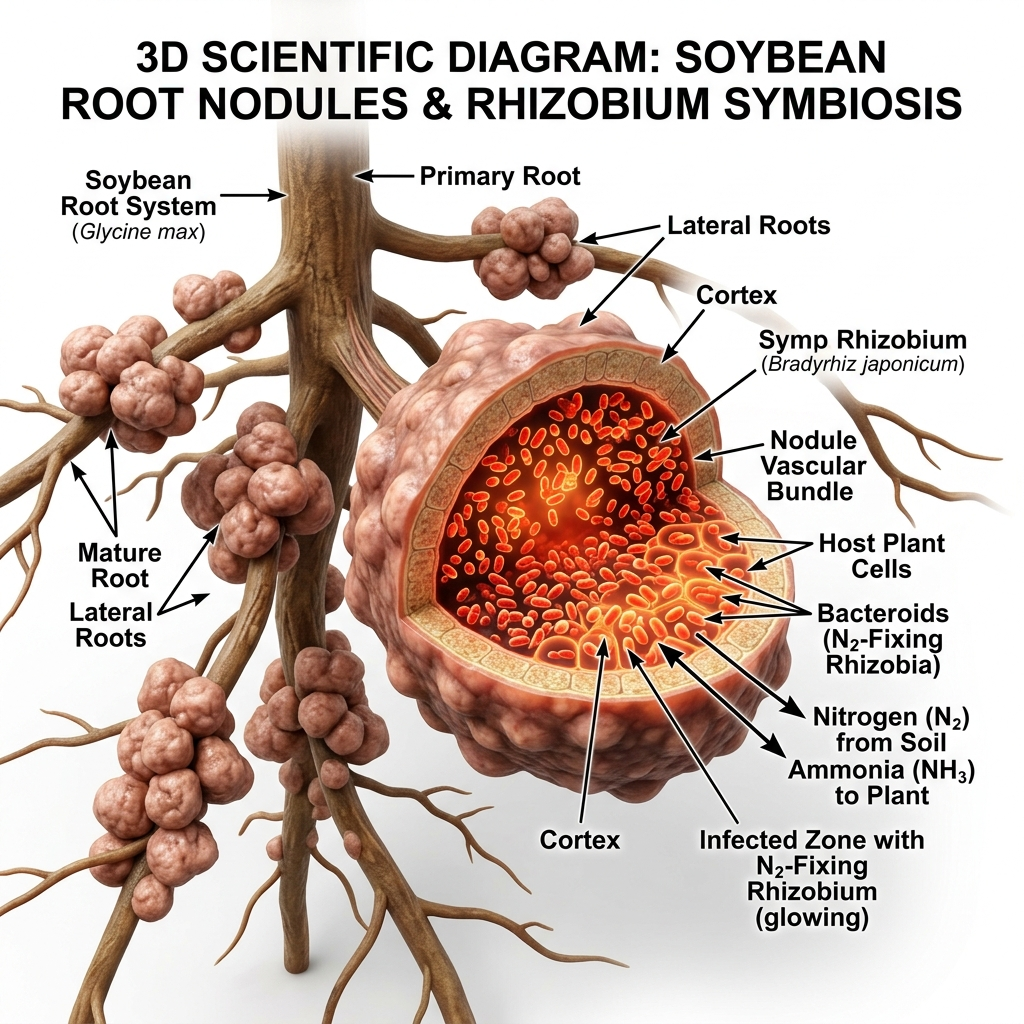
\includegraphics[width=0.85\textwidth]{assets/ch03_root_nodules.png}
    \caption{โครงสร้าง 3D ตัดขวางของปมรากพืชตระกูลถั่ว แสดงท่อติดเชื้อ (Infection thread) และกลุ่มเซลล์แบคทีรอยด์ (Bacteroids) ของเชื้อ \organism{Rhizobium} ด้านในเซลล์พืชที่ถูกห่อหุ้มในซิมไบโอโซม (Symbiosome) ล้อมรอบด้วยโปรตีนเลกเฮโมโกลบินสีแดง}
    \label{fig:ch03_root_nodules}
\end{figure}

\section*{วัตถุประสงค์การเรียนรู้ประจำบท}
เมื่อศึกษาบทเรียนนี้จบแล้ว นักศึกษาสามารถ:
\begin{enumerate}
    \item อธิบายความหมาย การจำแนกประเภท และความแตกต่างระหว่าง ePGPR และ iPGPR
    \item วิเคราะห์วิถีชีวเคมีของการสังเคราะห์ฮอร์โมนพืช (IAA) และกลไกการลดความเครียดพืชด้วยเอนไซม์ ACC Deaminase
    \item เปรียบเทียบความแตกต่างระหว่างระบบภูมิคุ้มกันพืช ISR (ชักนำโดย PGPR) และ SAR (ชักนำโดยเชื้อก่อโรค)
    \item อธิบายลำดับขั้นตอนโมเลกุลการส่งสัญญาณ Nod Factors ระหว่างพืชตระกูลถั่วกับ \organism{Rhizobium}
    \item วิเคราะห์บทบาทของเชื้อราอาร์บัสคูลาร์ไมคอร์ไรซา (AMF) ต่อการดูดซึมฟอสฟอรัสและการสร้างสารกลอมาลินในดิน
\end{enumerate}

\section{นิยามและการจัดจำแนกกลุ่ม PGPR}

คำว่า \textbf{PGPR (Plant Growth-Promoting Rhizobacteria)}\index{PGPR (Plant Growth-Promoting Rhizobacteria)} ถูกบัญญัติขึ้นครั้งแรกโดย Joseph W. Kloepper และ Milton N. Schroth ในปี ค.ศ. 1978 เพื่ออธิบายกลุ่มแบคทีเรียดินที่อาศัยอยู่หนาแน่นบริเวณรอบรากพืชและมีผลในการกระตุ้นการเจริญเติบโตของพืชอย่างชัดเจน จุลินทรีย์กลุ่มนี้จำแนกออกเป็น 2 กลุ่มใหญ่ตามความลึกของการอยู่อาศัยในเนื้อเยื่อพืช:

\begin{enumerate}
    \item \textbf{แบคทีเรียภายนอกเซลล์พืช (Extracellular PGPR: ePGPR):\index{ePGPR (Extracellular PGPR)}} ดำรงชีวิตอยู่บริเวณผิวสัมผัสราก (Rhizoplane) หรือในช่องว่างดินรอบราก (Rhizosphere) โดยไม่แทรกซึมเข้าไปในเนื้อเยื่อพืช ได้แก่ แบคทีเรียสกุล \organism{Pseudomonas}, \organism{Bacillus}, \organism{Azotobacter}, \organism{Azospirillum}, \organism{Serratia}, และ \organism{Streptomyces}
    \item \textbf{แบคทีเรียภายในเซลล์พืช (Intracellular PGPR: iPGPR):\index{iPGPR (Intracellular PGPR)}} สามารถแทรกซึมผ่านเซลล์ชั้นนอกเข้าไปอาศัยอยู่ภายในเซลล์เยื่อหุ้มของพืชอย่างจำเพาะเจาะจง โดยพืชจะสร้างอวัยวะพิเศษขึ้นมารองรับ ได้แก่ แบคทีเรียกลุ่มสร้างปมรากถั่วสกุล \organism{Rhizobium}, \organism{Bradyrhizobium}, \organism{Sinorhizobium}, และกลุ่มแอคติโนมัยซีสสร้างปมในพืชป่าสกุล \organism{Frankia}
\end{enumerate}

\section{กลไกส่งเสริมการเจริญเติบโตโดยตรง (Direct Mechanisms)}

\subsection{1. การสังเคราะห์ฮอร์โมนพืช (Phytohormone Biosynthesis)}

จุลินทรีย์ PGPR มากกว่าร้อยละ 80 มีความสามารถในการสังเคราะห์ฮอร์โมนพืชกลุ่มออกซิน โดยเฉพาะ \textbf{กรดอินโดล-3-อะซิติก (Indole-3-acetic acid: IAA)\index{กรดอินโดล-3-อะซิติก (IAA)}\index{Indole-3-acetic acid (IAA)}} ซึ่งแบคทีเรียใช้น้ำคั้นรากพืชที่มีกรดอะมิโนทริปโตเฟน (L-tryptophan) เป็นสารตั้งต้น ผ่าน 3 วิถีชีวเคมีหลัก:

\begin{itemize}
    \item \textbf{Indole-3-pyruvic acid (IPyA) Pathway:} เป็นวิถีหลักใน \organism{Pseudomonas} และ \organism{Azospirillum} โดยทริปโตเฟนถูกเปลี่ยนเป็น IPyA ด้วยเอนไซม์ Aminotransferase จากนั้นเปลี่ยนเป็น Indole-3-acetaldehyde (IAAld) และออกซิไดซ์เป็น IAA ในที่สุด
    \item \textbf{Indole-3-acetamide (IAM) Pathway:} พบเด่นชัดใน \organism{Agrobacterium} และ \organism{Pseudomonas syringae} ทริปโตเฟนถูกเปลี่ยนเป็น IAM ด้วยเอนไซม์ Tryptophan 2-monooxygenase และเปลี่ยนเป็น IAA ด้วยเอนไซม์ IAM hydrolase
    \item \textbf{Tryptamine (TAM) Pathway:} ทริปโตเฟนถูกเปลี่ยนเป็น Tryptamine ก่อนเปลี่ยนเป็น IAAld และ IAA
\end{itemize}

IAA ที่จุลินทรีย์หลั่งออกมาจะกระตุ้นการขยายตัวของเซลล์ราก (Cell Elongation) และส่งเสริมการแตกแขนงของรากฝอย (Lateral roots and root hairs) ซึ่งช่วยเพิ่มพื้นที่ผิวในการดูดซับน้ำและธาตุอาหารของพืชได้อย่างมหาศาล

\subsection{2. การลดความเครียดพืชด้วยเอนไซม์ ACC Deaminase}

เมื่อพืชประสบสภาวะเครียดจากสิ่งแวดล้อม เช่น ภัยแล้ง (Drought) ดินเค็ม (Salinity) หรือสารเคมีสะสม พืชจะสังเคราะห์ฮอร์โมนเอทิลีน (Ethylene) สูงขึ้นอย่างรวดเร็ว โดยผ่านสารตั้งต้นคือ \textbf{1-aminocyclopropane-1-carboxylic acid (ACC)} ฮอร์โมนเอทิลีนในระดับที่สูงเกินไป (Stress Ethylene)\index{เอทิลีนในสภาวะเครียด (Stress Ethylene)} จะสั่งการให้รากหยุดการยืดตัว ใบเหลือง และใบร่วงเฉับพลัน

\begin{equation}
\text{S-Adenosylmethionine (SAM)} \xrightarrow{\text{ACC Synthase}} \text{ACC} \xrightarrow{\text{ACC Oxidase}} \text{Ethylene}
\end{equation}

แบคทีเรีย PGPR ที่มีเอนไซม์ \textbf{ACC Deaminase\index{ACC Deaminase}} (เช่น \organism{Pseudomonas putida} สายพันธุ์ UW4) จะเข้าจับและสลายสาร ACC ที่รากพืชหลั่งออกมาให้แตกตัวเป็นสารที่ไม่เป็นพิษ:

\begin{equation}
\text{ACC} + H_2O \xrightarrow{\text{ACC Deaminase}} \alpha\text{-ketobutyrate} + NH_3
\end{equation}

แบคทีเรียจะนำแอมโมเนียและแอลฟา-คีโตบิวไทเรตไปใช้เป็นแหล่งไนโตรเจนและพลังงาน ส่งผลให้ความเข้มข้นของ ACC บริเวณรากลดลง เกิดแรงขับดันให้พืชส่ง ACC ออกมาสู่ภายนอกอย่างต่อเนื่อง ระดับเอทิลีนในพืชจึงลดลงสู่ระดับปกติ ทำให้ระบบรากสามารถเจริญเติบโตและทนแล้งทนเค็มได้ดีขึ้น

\begin{worked}[ตัวอย่างที่ 3.1 การคำนวณประสิทธิภาพการลดเอทิลีนและเพิ่มชีวมวลรากโดย ACC Deaminase]
ในการทดลองปลูกข้าวโพดในดินเค็ม ($EC = 8.5\text{ dS/m}$):
\begin{itemize}
    \item ชุดควบคุม (ไม่อินอคูเลตเชื้อ): พืชสะสมเอทิลีนในใบ $12.8\text{ nmol/g FW/hr}$ มีน้ำหนักแห้งราก $1.45\text{ g/ต้น}$
    \item ชุดทดลอง (อินอคูเลต \organism{Pseudomonas putida} ที่มี ACC Deaminase สูง): พืชสะสมเอทิลีนลดลงเหลือ $6.4\text{ nmol/g FW/hr}$ มีน้ำหนักแห้งรากเพิ่มขึ้นเป็น $2.32\text{ g/ต้น}$
\end{itemize}
จงคำนวณร้อยละการลดลงของเอทิลีนสะสม และร้อยละการเพิ่มขึ้นของชีวมวลราก

\textbf{วิธีทำ:}
1. ร้อยละการลดลงของเอทิลีน:
$$\% \text{ Ethylene Reduction} = \frac{12.8 - 6.4}{12.8} \times 100 = 50.0\%$$
2. ร้อยละการเพิ่มขึ้นของชีวมวลราก:
$$\% \text{ Root Biomass Increase} = \frac{2.32 - 1.45}{1.45} \times 100 = \frac{0.87}{1.45} \times 100 = 60.0\%$$

\textbf{บทวิเคราะห์ผลลัพธ์:} การใช้แบคทีเรียสร้างเอนไซม์ ACC Deaminase สามารถยับยั้งการสร้างเอทิลีนสภาวะเครียดได้ถึงครึ่งหนึ่ง ส่งผลให้ระบบรากสามารถแผ่ขยายเพิ่มขึ้นถึง 60\% ทำให้พืชดูดน้ำและธาตุอาหารในดินเค็มได้อย่างมีประสิทธิภาพ
\end{worked}

\section{กลไกส่งเสริมการเจริญเติบโตโดยอ้อม (Indirect Mechanisms)}

\subsection{1. สารไซเดอโรฟอร์ (Siderophores) และการแย่งชิงธาตุเหล็ก}

ในสภาวะที่มีออกซิเจนและค่า pH เป็นกลางถึงด่าง เหล็กในดินจะอยู่ในรูปเฟอร์ริกไอออน ($Fe^{3+}$) ซึ่งตกตะกอนเป็นสารประกอบออกไซด์และไฮดรอกไซด์ที่ไม่ละลายน้ำ ($\text{Solubility } \approx 10^{-18}\text{ M}$) จุลินทรีย์ PGPR จะหลั่งสารอินทรีย์น้ำหนักโมเลกุลต่ำ (400--1,500 Da) ที่เรียกว่า \textbf{ไซเดอโรฟอร์ (Siderophores)\index{ไซเดอโรฟอร์ (Siderophores)}} ซึ่งมีค่าคงที่การจับเหล็กที่สูงมาก ($\log K_f > 30$) เช่น ไพโอเวอร์ดีน (Pyoverdine)\index{ไพโอเวอร์ดีน (Pyoverdine)} ใน \organism{Pseudomonas fluorescens} และบาซิลโลแบคติน (Bacillibactin) ใน \organism{Bacillus subtilis}

แบคทีเรีย PGPR จะแย่งจับไอออนเหล็กในไรโซสเฟียร์ไปอย่างรวดเร็ว ทำให้เชื้อราก่อโรคพืช เช่น \organism{Fusarium oxysporum} และ \organism{Pythium ultimum} ขาดแคลนธาตุเหล็กที่จำเป็นต่อกระบวนการหายใจระดับเซลล์และการงอกของสปอร์ จึงไม่สามารถเข้าทำลายรากพืชได้

\subsection{2. การชักนำความต้านทานโรคทั้งระบบของพืช (ISR vs SAR)}

พืชมีระบบภูมิคุ้มกันระดับทั้งต้น 2 รูปแบบที่ถูกควบคุมโดยฮอร์โมนและวิถีการส่งสัญญาณที่แตกต่างกันอย่างสิ้นเชิง:\index{Induced Systemic Resistance (ISR)}\index{Systemic Acquired Resistance (SAR)}

\begin{table}[ht]
\centering
\small
\begin{tabular}{lp{4.2cm}p{4.2cm}}
\toprule
\textbf{คุณลักษณะ} & \textbf{Induced Systemic Resistance (ISR)} & \textbf{Systemic Acquired Resistance (SAR)} \\
\midrule
สิ่งมีชีวิตผู้ชักนำ & จุลินทรีย์ที่เป็นประโยชน์ (PGPR, ไมคอร์ไรซา, \organism{Trichoderma}) & เชื้อก่อโรคพืช (เชื้อรา, แบคทีเรีย, ไวรัส) \\
อาการเนื้อเยื่อพืช & ไม่เกิดแผลเนื้อเยื่อตาย (Non-necrotic) & เกิดแผลเนื้อเยื่อตายเฉพาะจุด (Hypersensitive Response: HR) \\
ฮอร์โมนส่งสัญญาณ & กรดจัสโมนิก (Jasmonic Acid) และเอทิลีน (Ethylene) & กรดซาลิไซลิก (Salicylic Acid: SA) \\
โปรตีนควบคุมหลัก & NPR1 (ทำงานในไซโทพลาสซึมร่วมกับวิถี JA/ET) & NPR1 (เคลื่อนย้ายเข้าสู่นิวเคลียสกระตุ้นยีน PR) \\
โปรตีนป้องกันตัว & สะสมเอนไซม์ป้องกันตัวล่วงหน้า (Priming State: LOX, POD) & สร้างโปรตีน Pathogenesis-Related (PR proteins: PR-1, PR-5) \\
\bottomrule
\end{tabular}
\caption{การเปรียบเทียบเชิงวิเคราะห์ระหว่างระบบภูมิคุ้มกันพืช ISR และ SAR}
\label{tab:isr_vs_sar}
\end{table}

\section{ความสัมพันธ์ระดับโมเลกุลระหว่างพืชตระกูลถั่วกับ Rhizobium}

ความสัมพันธ์แบบพึ่งพาอาศัยกันระหว่างพืชตระกูลถั่วและแบคทีเรีย \organism{Rhizobium} เป็นหนึ่งในระบบส่งสัญญาณทางชีวภาพที่มีความจำเพาะสูงที่สุดในธรรมชาติ:

\begin{enumerate}
    \item \textbf{การหลั่งสารฟลาโวนอยด์ (Flavonoids Exudation):} รากพืชหลั่งสารกลุ่มฟลาโวนอยด์และไอโซฟลาโวนอยด์ (เช่น Luteolin, Daidzein, Genistein) ออกสู่ไรโซสเฟียร์
    \item \textbf{การกระตุ้นยีนสร้างปม (Nod Gene Activation):} ฟลาโวนอยด์เข้าจับกับโปรตีนควบคุม NodD ของแบคทีเรีย กระตุ้นให้เกิดการถอดรหัสของยีนกลุ่ม \genus{nodABC}
    \item \textbf{การสังเคราะห์และหลั่ง Nod Factors:} แบคทีเรียสังเคราะห์สารลิโพไคตินโอลิโกแซกคาไรด์ (Lipochitooligosaccharides: LCOs หรือ Nod factors)\index{Nod Factors} ซึ่งมีโครงสร้างแกนหลักเป็น $\beta$-1,4-linked N-acetylglucosamine และมีสายโซ่กรดไขมันจำเพาะ
    \item \textbf{การม้วนงอของขนราก (Root Hair Curling):} Nod factor เข้าจับกับตัวรับ Nod Factor Receptors (NFR1/NFR5) ที่เยื่อหุ้มเซลล์ขนราก กระตุ้นการไหลเวียนของแคลเซียม ($Ca^{2+}$ spiking) ส่งผลให้ขนรากม้วนงอเป็นรูปตะขอ (Shepherd's crook) ดักจับเซลล์แบคทีเรีย
    \item \textbf{การสร้างท่อติดเชื้อ (Infection Thread):} แบคทีเรียแทรกผ่านผนังเซลล์และสร้างท่อติดเชื้อเคลื่อนตัวเข้าสู่เปลือกราก (Cortex) กระตุ้นให้เซลล์พืชแบ่งตัวกลายเป็นปมราก (Root Nodule)
    \item \textbf{การเปลี่ยนสภาพเป็นแบคทีรอยด์ (Bacteroid Differentiation):} แบคทีเรียหลุดออกจากท่อติดเชื้อเข้าสู่เซลล์พืช ถูกห่อหุ้มด้วยเยื่อหุ้มของพืชกลายเป็น \textbf{ซิมไบโอโซม (Symbiosome)\index{ซิมไบโอโซม (Symbiosome)}} แบคทีเรียขยายขนาดและเปลี่ยนรูปร่างเป็นแบคทีรอยด์ (Bacteroids)\index{แบคทีรอยด์ (Bacteroids)} และเริ่มสังเคราะห์เอนไซม์ไนโตรจีเนสเพื่อตรึงไนโตรเจนภายใต้การปกป้องของโปรตีนเลกเฮโมโกลบิน
\end{enumerate}

\section{เชื้อราอาร์บัสคูลาร์ไมคอร์ไรซา (AMF) และการดูดซับฟอสฟอรัส}

เชื้อราอาร์บัสคูลาร์ไมคอร์ไรซา (Arbuscular Mycorrhizal Fungi: AMF\index{Arbuscular Mycorrhizal Fungi (AMF)}\index{ราไมคอร์ไรซา (Mycorrhizal Fungi)} ในไฟลัม Glomeromycota เช่น สกุล \organism{Glomus}, \organism{Rhizophagus}) สร้างความสัมพันธ์แบบพึ่งพาอาศัยกับรากพืชบกร้อยละ 80 

เส้นใยภายในรากจะแทรกผ่านผนังเซลล์เปลือกรากเข้าไปสร้างโครงสร้างแตกกิ่งก้านคล้ายต้นไม้จิ๋วที่เรียกว่า \textbf{อาร์บัสคูล (Arbuscules)\index{อาร์บัสคูล (Arbuscules)}} ซึ่งเป็นจุดแลกเปลี่ยนสารอาหารหลักระหว่างเชื้อรากับพืช โดยเชื้อราส่งผ่านฟอสเฟตไอออน ($H_2PO_4^-$) สังกะสี และทองแดงให้แก่พืช แลกเปลี่ยนกับน้ำตาลและลิพิดที่ได้จากการสังเคราะห์แสงของพืช

นอกจากนี้ เส้นใยภายนอกราก (Extraradical Hyphae) ที่แผ่ขยายออกไปในดินได้ไกลหลายสิบเซนติเมตร ยังทำหน้าที่หลั่งโปรตีนไกลโคโปรตีนที่ไม่ละลายน้ำที่เรียกว่า \textbf{กลอมาลิน (Glomalin)\index{กลอมาลิน (Glomalin)}} ซึ่งทำหน้าที่เป็นกาวธรรมชาติเชื่อมอนุภาคดินเหนียวและทรายให้เกาะกันเป็นเม็ดดินที่มั่นคง (Stable Soil Aggregates) ช่วยเพิ่มความสามารถในการกักเก็บน้ำและคาร์บอนในดินอย่างถาวร

\section{แผนผังกลไกชีวโมเลกุลและการตรึงไนโตรเจนทางชีวภาพของ PGPR}
\index{Biological Nitrogen Fixation@Biological Nitrogen Fixation (การตรึงไนโตรเจนทางชีวภาพ)}\index{Rhizobium@Rhizobium}\index{Indole-3-Acetic Acid@Indole-3-Acetic Acid (IAA)}

กลุ่มแบคทีเรียส่งเสริมการเจริญเติบโตของพืช (PGPR) ประสานการทำงานผ่านกลไกพหุหน้าที่ (Multifunctional Traits) ดังแสดงในแผนผังสถาปัตยกรรมชีวภาพ:

\begin{figure}[ht]
\centering
\begin{tikzpicture}[node distance=1.4cm, >=Stealth]
    \node[draw=mbGreen!80!black, fill=mbGreen!15, rounded corners, minimum width=3.5cm, align=center] (pgpr) {\textbf{PGPR ในบริเวณไรโซสเฟียร์}\\\textit{Pseudomonas}, \textit{Bacillus}};
    \node[draw=navyprimary, fill=mbLightGreen!30, rounded corners, above left=1.2cm of pgpr, text width=3.0cm, align=center] (iaa) {\textbf{การผลิตฮอร์โมน}\\IAA, Gibberellin\\กระตุ้นการแตกราก};
    \node[draw=navyprimary, fill=mbCyan!15, rounded corners, above right=1.2cm of pgpr, text width=3.0cm, align=center] (p_sol) {\textbf{การละลายฟอสเฟต}\\กรดอินทรีย์ + Phosphatase\\ปลดปล่อย $PO_4^{3-}$};
    \node[draw=mbAmber!80!black, fill=mbAmber!20, rounded corners, below=1.2cm of pgpr, text width=4.5cm, align=center] (biocontrol) {\textbf{การควบคุมศัตรูพืชชีวภาพ}\\Siderophore แย่งจับเหล็ก\\สารปฏิชีวนะยับยั้งเชื้อราก่อโรค};

    \draw[->, thick, color=mbGreen!80!black] (pgpr) -- (iaa);
    \draw[->, thick, color=mbGreen!80!black] (pgpr) -- (p_sol);
    \draw[->, thick, color=mbAmber!80!black] (pgpr) -- (biocontrol);
\end{tikzpicture}
\caption{แผนผังกลไกการส่งเสริมการเจริญเติบโตของพืชและควบคุมโรคทางชีวภาพโดย PGPR}
\label{fig:pgpr_mechanisms}
\end{figure}

\begin{table}[ht]
\centering
\small
\begin{tabular}{lp{3.8cm}p{4.5cm}}
\toprule
\textbf{กลุ่มสายพันธุ์ PGPR} & \textbf{กลไกเด่น} & \textbf{ประโยชน์ในภาคสนาม} \\
\midrule
\textit{Rhizobium} spp. & การตรึงไนโตรเจนแบบพึ่งพาอาศัย & สร้างปมรากในพืชตระกูลถั่ว ลดการใช้ปุ๋ยยูเรีย \\
\textit{Bacillus subtilis} & ผลิต Lipopeptides (Surfactin) & ยับยั้งเชื้อราโรครากเน่าและโรคแอนแทรคโนส \\
\textit{Pseudomonas fluorescens} & สังเคราะห์ Siderophore (Pyoverdine) & ชิงไอออนเหล็ก ยับยั้งเชื้อราโรคพืชในดิน \\
\bottomrule
\end{tabular}
\caption{ตารางเปรียบเทียบคุณสมบัติของสายพันธุ์ PGPR ในการประยุกต์ใช้ในแปลงเกษตรอัจฉริยะ}
\label{tab:pgpr_strains}
\end{table}

% [RESEARCH-UPDATE-2026-10]
\section{ความก้าวหน้างานวิจัยล่าสุดด้านแบคทีเรียส่งเสริมการเจริญเติบโตของพืช}

งานวิจัยระดับนานาชาติในปี ค.ศ. 2023–2025 โดย Chieb และ Gachomo \cite{pmid37626328} ได้ทบทวนกลไกของ PGPR ในการตอบสนองต่อสภาวะแล้ง โดยเน้นย้ำถึงการปรับปรุงโครงสร้างของระบบรากและการกระตุ้นการสร้างสารออสโมโพรเทกแทนท์ (Osmoprotectants: เช่น Proline และ Glycine betaine) ในใบพืช 

ร่วมกับงานวิจัยของ de Andrade และคณะ \cite{pmid37110511} ที่พิสูจน์ว่าการใช้อินอคูเลชันร่วมระหว่างแบคทีเรียตรึงไนโตรเจน \organism{Azospirillum brasilense} กับแบคทีเรียละลายฟอสเฟต \organism{Bacillus} สามารถเพิ่มผลผลิตข้าวโพดและถั่วเหลืองในแปลงเกษตรจริงได้มากกว่าร้อยละ 20 พร้อมลดการใช้ปุ๋ยเคมีลงถึงหนึ่งในสาม

\begin{insight}[ประเด็นวิเคราะห์เชิงวิชาการ]
เกษตรกรผู้ปลูกทุเรียนมักประสบปัญหาการเน่าเสียของรากฝอยในช่วงฤดูฝนเนื่องจากเชื้อราก่อโรคในดิน หากเราต้องการออกแบบสูตรหัวเชื้อจุลินทรีย์ร่วม (Consortium) เพื่อใส่ในทรงพุ่มทุเรียน เราควรเลือกจุลินทรีย์ที่มีกลไกใดทำงานประสานกันบ้าง?
\end{insight}

\begin{application}[กรณีศึกษางานวิจัย RBRU: การประยุกต์ใช้กลุ่มจุลินทรีย์ PGPR ท้องถิ่นในสวนทุเรียน จ.จันทบุรี]
จากงานวิจัยของ Jantamalee \& Thassana (2025) \cite{jantamalee_2025} และ Jantamalee \& Thassana (2026) \cite{jantamalee_2026_biotech} ณ มหาวิทยาลัยราชภัฏรำไพพรรณี\index{งานวิจัย RBRU!จุลินทรีย์ดินสวนทุเรียน} ได้ทำการสำรวจและคัดแยกแบคทีเรีย PGPR ประจำถิ่นจากดินไรโซสเฟียร์สวนทุเรียนพันธุ์หมอนทองในพื้นที่ อ.เขาคิชฌกูฏ และ อ.โป่งน้ำร้อน จ.จันทบุรี พบสายพันธุ์เด่น \organism{Bacillus velezensis}\index{Bacillus velezensis@\textit{Bacillus velezensis}} สายพันธุ์ RBRU-B01 และ \organism{Azospirillum brasilense}\index{Azospirillum brasilense@\textit{Azospirillum brasilense}} สายพันธุ์ RBRU-A03 

เมื่อนำมาทดสอบแบบ Consortium\index{Consortium!PGPR ท้องถิ่น} ร่วมกันในระยะต้นกล้าทุเรียน พบผลลัพธ์เชิงประจักษ์:
\begin{itemize}
    \item \textbf{การสร้างออกซินและการแตกราก:} มีการหลั่งฮอร์โมน IAA สูงถึง $42.8 \pm 3.1\text{ mg/L}$ ในหลอดทดลอง ส่งผลให้พื้นที่ผิวรากฝอย (Root Surface Area) ของต้นกล้าทุเรียนเพิ่มขึ้นร้อยละ $38.4\%$ เมื่อเทียบกับชุดควบคุม
    \item \textbf{การละลายฟอสเฟต:} ละลายหินฟอสเฟตในดินเหนียวทุเรียนได้ค่าฟอสฟอรัสที่เป็นประโยชน์ (Available P) เพิ่มขึ้นจาก $12.5\text{ mg/kg}$ เป็น $28.6\text{ mg/kg}$ ภายใน 30 วัน
    \item \textbf{การกระตุ้นเอนไซม์ต้านทานโรค (Priming Defense):} ระดับกิจกรรมของเอนไซม์ Peroxidase (POD)\index{เอนไซม์เพอร์ออกซิเดส (POD)} และ Polyphenol Oxidase (PPO)\index{เอนไซม์พอลิฟีนอลออกซิเดส (PPO)} ในใบเพิ่มขึ้น $2.4$ เท่า ช่วยลดความเสี่ยงจากการเข้าทำลายของโรครากเน่าโคนเน่าได้อย่างมีนัยสำคัญทางสถิติ ($p < 0.01$)
\end{itemize}
\end{application}

\section*{สรุปประจำบท}

PGPR และเชื้อราไมคอร์ไรซาเป็นพันธมิตรทางชีววิทยาที่ทรงพลังที่สุดของระบบรากพืช การกระตุ้นการเจริญเติบโตดำเนินไปผ่านวิถีเคมีชีวภาพที่แม่นยำ ทั้งการสังเคราะห์ออกซิน (IAA) การยับยั้งเอทิลีนสภาวะเครียดด้วยเอนไซม์ ACC Deaminase และการส่งสัญญาณระดับยีนระหว่างพืชตระกูลถั่วกับ \organism{Rhizobium} นอกจากนี้ กลไกการแย่งชิงเหล็กด้วยไซเดอโรฟอร์และการกระตุ้นภูมิคุ้มกัน ISR ช่วยสร้างปราการป้องกันโรคพืชโดยไม่ต้องพึ่งพาสารเคมี การผสานสายพันธุ์จุลินทรีย์เหล่านี้เข้าเป็นสูตรชีวภัณฑ์ผสมผสานถือเป็นกุญแจสำคัญสู่ความยั่งยืนทางการเกษตร

\subsection*{คำถามท้ายบทและการวิเคราะห์}

\noindent \textbf{ระดับที่ 1: ความรู้และความเข้าใจเชิงทฤษฎี (Knowledge \& Comprehension)}
\begin{enumerate}
    \item เปรียบเทียบความแตกต่างระหว่าง ePGPR และ iPGPR พร้อมยกตัวอย่างแบคทีเรียในแต่ละกลุ่มมาอย่างละ 2 สกุล
    \item อธิบายวิถีชีวเคมี IPyA ในการสังเคราะห์ฮอร์โมน Indole-3-Acetic Acid (IAA) ของแบคทีเรีย \organism{Pseudomonas}
    \item เอนไซม์ ACC Deaminase มีกลไกการทำงานอย่างไรในการช่วยให้พืชรอดพ้นจากสภาวะแล้งและดินเค็ม?
    \item เปรียบเทียบระบบภูมิคุ้มกันพืช ISR (Induced Systemic Resistance) และ SAR (Systemic Acquired Resistance) ในแง่ของสิ่งมีชีวิตผู้ชักนำ ฮอร์โมนควบคุม และลักษณะอาการของพืช
\end{enumerate}

\noindent \textbf{ระดับที่ 2: การวิเคราะห์และการคำนวณเชิงปริมาณ (Quantitative Analysis \& Calculation)}
\begin{enumerate}[resume]
    \item อธิบายบทบาทของสารไซเดอโรฟอร์ (Siderophores) ในการแย่งชิงธาตุเหล็กจากเชื้อราก่อโรคพืชในดิน พร้อมเขียนสมการสมดุลการจับไอออน $Fe^{3+}$
    \item ลำดับขั้นตอนการส่งสัญญาณทางเคมีระหว่างรากพืชตระกูลถั่วกับ \organism{Rhizobium} เริ่มต้นตั้งแต่การหลั่งสารฟลาโวนอยด์จนถึงการสร้างปมราก
    \item ในการคำนวณ Phosphate Solubilization Index (PSI) หากอาณานิคมโคโลนีมีเส้นผ่านศูนย์กลาง $8.0\text{ mm}$ และวงใสมีเส้นผ่านศูนย์กลาง $20.0\text{ mm}$ จงคำนวณหาค่า PSI และวิเคราะห์ระดับประสิทธิภาพ
\end{enumerate}

\noindent \textbf{ระดับที่ 3: การสังเคราะห์และการแก้ปัญหาในแปลงจริง (Application \& Real-World Synthesis)}
\begin{enumerate}[resume]
    \item เชื้อราอาร์บัสคูลาร์ไมคอร์ไรซา (AMF) มีกลไกอย่างไรในการช่วยให้พืชดูดซับธาตุฟอสฟอรัสที่ละลายน้ำยากในดิน และสารกลอมาลินช่วยปรับปรุงฟิสิกส์ดินอย่างไร?
    \item จากกรณีศึกษางานวิจัย RBRU ในสวนทุเรียน จ.จันทบุรี จงอธิบายประโยชน์ของการใช้ PGPR แบบ Consortium ระหว่าง \organism{Bacillus} และ \organism{Azospirillum} เหนือกว่าการใช้หัวเชื้อเดี่ยว
    \item ในการออกแบบหัวเชื้อจุลินทรีย์ร่วม (Consortium) เพื่อส่งเสริมการเจริญเติบโตของพืช เหตุใดเราจึงไม่ควรนำจุลินทรีย์ปฏิปักษ์ที่หลั่งสารฆ่าเชื้อราชนิดรุนแรงมาผสมกับเชื้อราไมคอร์ไรซาในถังเดียวกันโดยตรง?
\end{enumerate}

\chapter{โรคพืชที่เกิดจากจุลินทรีย์ กลไกระดับโมเลกุล และระบาดวิทยา}
\label{ch:plant_pathogens}

\begin{keyconcept}[แนวคิดสำคัญของบทที่ 4]
โรคพืชที่เกิดจากจุลินทรีย์สร้างความเสียหายทางเศรษฐกิจแก่ผลผลิตการเกษตรทั่วโลกมากกว่าร้อยละ 20--40 ต่อปี การเกิดโรคเป็นผลลัพธ์ของปฏิสัมพันธ์ 3 มิติใน "สามเหลี่ยมการเกิดโรคพืช" (Disease Triangle) ระหว่างพืชเจ้าบ้านที่อ่อนแอ จุลินทรีย์ก่อโรคที่มีความรุนแรง และสภาวะแวดล้อมที่เอื้ออำนวย ในระดับโมเลกุล การต่อสู้ระหว่างพืชและเชื้อก่อโรคดำเนินไปตามแบบจำลองทางภูมิคุ้มกันวิทยา "Zigzag Model" ซึ่งขับเคี่ยวระหว่างภูมิคุ้มกันกระตุ้นด้วยสารโมเลกุลก่อโรค (PTI) และการหลั่งโปรตีนแทรกซึม (Effectors) ผ่านระบบหลั่งสาร เช่น Type III Secretion System (T3SS) จนนำไปสู่ภูมิคุ้มกันตอบสนองจำเพาะ (ETI) การผสานแบบจำลองคณิตศาสตร์ระบาดวิทยา (AUDPC และ Logistic Model) ร่วมกับเทคโนโลยี Edge AI วิทัศน์คอมพิวเตอร์ ช่วยให้ตรวจจับและควบคุมการระบาดของโรคได้อย่างแม่นยำตั้งแต่ระยะเริ่มแรก
\end{keyconcept}

\begin{figure}[ht]
    \centering
    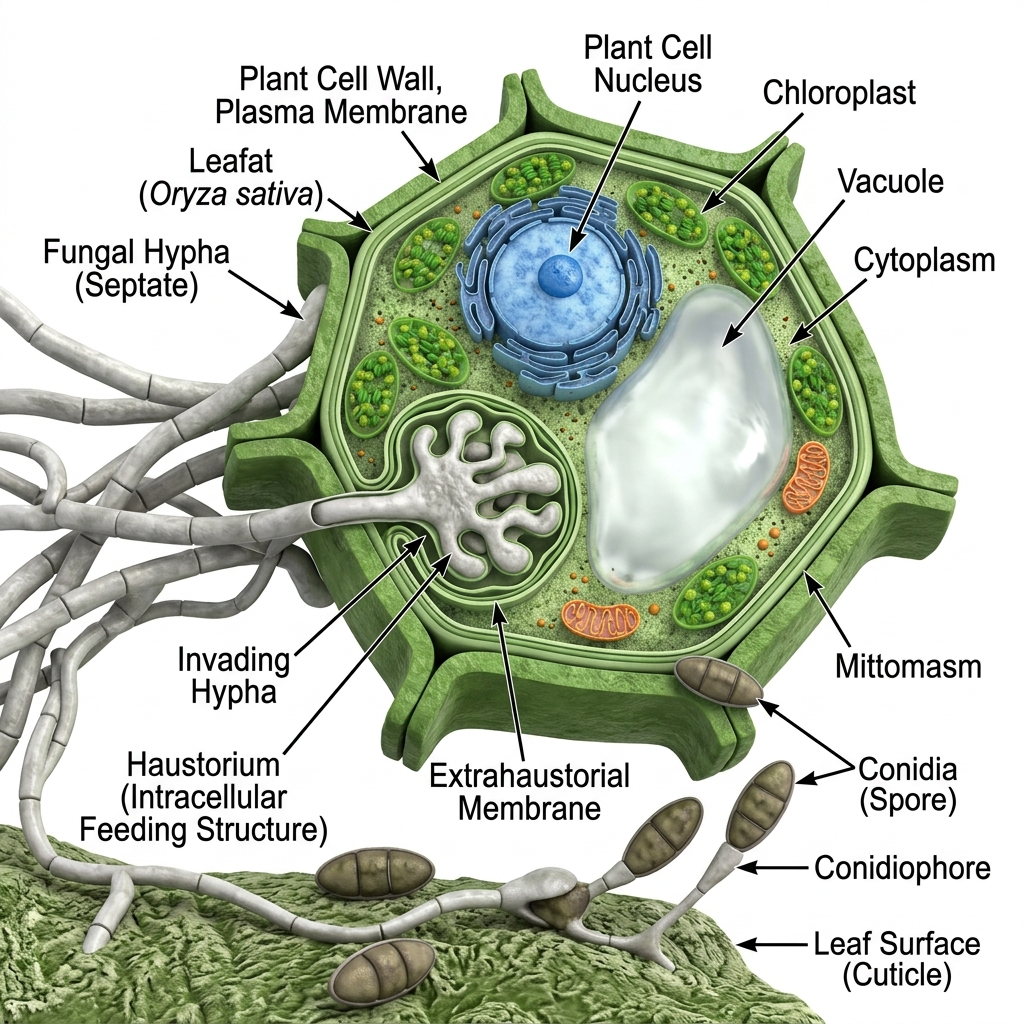
\includegraphics[width=0.85\textwidth]{assets/ch04_fungal_infection.png}
    \caption{การจำลองภาพ 3D ขยายส่วนปลายใยรา (Hypha) ขณะพัฒนาโครงสร้างแอพเพรสโซเรียม (Appressorium) สร้างแรงดันเต่งมหาศาล ส่งเข็มเจาะ (Penetration peg) ทะลุผนังเซลล์พืช และแผ่ขยายสายใยดูดซึมอาหารโฮสทอเรียม (Haustorium) โอบล้อมด้วยเยื่อหุ้มเซลล์โฮสต์โดยไม่ทำให้เยื่อหุ้มเซลล์แตกสลาย}
    \label{fig:ch04_fungal_infection}
\end{figure}

\section*{วัตถุประสงค์การเรียนรู้ประจำบท}
เมื่อศึกษาบทเรียนนี้จบแล้ว นักศึกษาสามารถ:
\begin{enumerate}
    \item อธิบายองค์ประกอบของสามเหลี่ยมการเกิดโรคพืช และพีระมิดโรคพืชที่บูรณาการมิติกาลเวลาและมนุษย์
    \item วิเคราะห์กลไกภูมิคุ้มกันพืชตามแบบจำลอง Zigzag Model (PTI vs ETS vs ETI) และระบบหลั่งสารของแบคทีเรียก่อโรค (T3SS, T4SS, T6SS)
    \item จำแนกสรีรวิทยาและกลไกการเข้าทำลายของเชื้อราแท้ ออยคาร์พิก (Oomycetes: \organism{Phytophthora}) แบคทีเรียท่อน้ำ และไวรัสพืช
    \item คำนวณแบบจำลองคณิตศาสตร์ระบาดวิทยา Monomolecular, Logistic และพื้นที่ใต้กราฟความรุนแรงของโรค (AUDPC)
    \item ประยุกต์ใช้เทคโนโลยี Edge AI และอัลกอริทึมวิทัศน์คอมพิวเตอร์ในการคัดกรองและประเมินระดับความรุนแรงของโรคพืชในแปลงเกษตรจริง
\end{enumerate}

\section{นิเวศวิทยาการเกิดโรค: สามเหลี่ยมและพีระมิดการเกิดโรคพืช}

การเกิดโรคในพืชไม่ได้ขึ้นอยู่กับเพียงแค่การมีอยู่ของเชื้อจุลินทรีย์เท่านั้น แต่เป็นปรากฏการณ์ทางนิเวศวิทยาที่ต้องอาศัยความสอดคล้องพร้อมกันของปัจจัยพื้นฐาน 3 ประการ ซึ่งรู้จักกันในนาม \textbf{สามเหลี่ยมการเกิดโรคพืช (Disease Triangle)\index{สามเหลี่ยมการเกิดโรคพืช (Disease Triangle)}}:

\begin{enumerate}
    \item \textbf{พืชเจ้าบ้านที่อ่อนแอ (Susceptible Host):} ระดับความอ่อนแอแปรผันตามพันธุกรรม อายุของพืช สภาพความสมบูรณ์ และระยะการเจริญเติบโต (เช่น ยอดอ่อนและผลอ่อนมักอ่อนแอกว่าใบแก่)
    \item \textbf{เชื้อก่อโรคที่มีความรุนแรงสูง (Virulent Pathogen):} ปริมาณหัวเชื้อเริ่มต้น (Inoculum density) ความสามารถในการสร้างสารพิษ เอนไซม์ย่อยผนังเซลล์ และความเร็วในการแบ่งตัวขยายพันธุ์
    \item \textbf{สภาพแวดล้อมที่เอื้ออำนวย (Favorable Environment):} อุณหภูมิ ความชื้นสัมพัทธ์ในอากาศ (RH $> 85\%$) ปริมาณน้ำฝน ความชื้นในดิน ค่า pH และการได้รับแสงแดด
\end{enumerate}

ในทางการเกษตรยุคใหม่ แบบจำลองสามเหลี่ยมได้รับการขยายเป็น \textbf{พีระมิดการเกิดโรคพืช (Disease Pyramid)\index{พีระมิดการเกิดโรคพืช (Disease Pyramid)}} โดยเพิ่มอีก 2 มิติสำคัญ:
\begin{itemize}
    \item \textbf{มิติของเวลา (Time):} ระยะเวลาที่พืชและเชื้อสัมผัสกันภายใต้สภาพแวดล้อมที่เหมาะสม ความถี่ของการเกิดหยดน้ำบนใบ (Leaf wetness duration)
    \item \textbf{กิจกรรมและการจัดการของมนุษย์ (Human Activity):} การปลูกพืชเชิงเดี่ยว (Monoculture) สายพันธุ์เดียวกันทั้งแปลง การให้ปุ๋ยไนโตรเจนมากเกินไปจนเนื้อเยื่อพืชอวบน้ำและอ่อนแอ ระบบการให้น้ำแบบสปริงเกอร์ที่กระจายสปอร์เชื้อรา และการเคลื่อนย้ายต้นพันธุ์ข้ามเขตแดน
\end{itemize}

\section{ภูมิคุ้มกันระดับโมเลกุลของพืช: แบบจำลอง Zigzag Model}

พืชไม่มีระบบภูมิคุ้มกันแบบแอนติบอดี (Adaptive Immune System) เหมือนสัตว์มีกระดูกสันหลัง แต่มีระบบภูมิคุ้มกันภายในระดับเซลล์ (Innate Immunity) ที่ซับซ้อน ซึ่งนักชีววิทยาพืช Jonathan Jones และ Jeffery Dangl (2006) ได้สรุปไว้เป็นแบบจำลองที่มีชื่อเสียงเรียกว่า \textbf{Zigzag Model\index{Zigzag Model of Plant Immunity}}:

\begin{figure}[ht]
\centering
\resizebox{0.96\textwidth}{!}{
\begin{tikzpicture}
    % Axes
    \draw[->, thick] (0,0) -- (12,0) node[right] {\textbf{เวลา (Time)}};
    \draw[->, thick] (0,0) -- (0,6) node[above] {\textbf{ภูมิคุ้มกัน (Amplitude)}};
    
    % Defense Thresholds
    \draw[dashed, red, thick] (0,2.5) -- (11.5,2.5);
    \node[red, font=\footnotesize\bfseries, above] at (6, 2.5) {ขีดขั้นการต้านทานโรค (Resistance Threshold)};
    
    % Zigzag Curve
    % Phase 1: PTI
    \draw[line width=1.8pt, blue] (0,0.5) -- (2.5,3.8) node[midway, above left, blue] {\textbf{1. PTI}};
    % Phase 2: ETS
    \draw[line width=1.8pt, red!80!black] (2.5,3.8) -- (5.0,1.2) node[midway, above right, red!80!black] {\textbf{2. ETS}};
    % Phase 3: ETI
    \draw[line width=1.8pt, forestgreen] (5.0,1.2) -- (8.0,5.5) node[midway, above left, forestgreen] {\textbf{3. ETI (HR)}};
    % Phase 4: Pathogen Evolution
    \draw[line width=1.8pt, orange] (8.0,5.5) -- (10.5,2.0) node[midway, above right, orange] {\textbf{4. Effector Div.}};
    \draw[line width=1.8pt, purple] (10.5,2.0) -- (11.8,4.8);
    
    % Labels below
    \node[draw, fill=blue!10, rounded corners, text width=2.4cm, align=center] at (1.5,-1.2) {\footnotesize \textbf{ระยะที่ 1}\\พืชตรวจจับ PAMPs ด้วย PRRs};
    \node[draw, fill=red!10, rounded corners, text width=2.4cm, align=center] at (4.5,-1.2) {\footnotesize \textbf{ระยะที่ 2}\\เชื้อหลั่ง Effectors ยับยั้ง PTI};
    \node[draw, fill=green!10, rounded corners, text width=2.4cm, align=center] at (7.8,-1.2) {\footnotesize \textbf{ระยะที่ 3}\\NBS-LRR จำจับ Effectors เกิด HR};
    \node[draw, fill=orange!10, rounded corners, text width=2.4cm, align=center] at (10.8,-1.2) {\footnotesize \textbf{ระยะที่ 4}\\เชื้อวิวัฒน์หลบหลีก พืชสร้าง R ใหม่};
\end{tikzpicture}
}
\caption{แบบจำลอง Zigzag Model แสดงการชิงไหวชิงพริบทางวิวัฒนาการระหว่างระบบภูมิคุ้มกันของพืชกับสารก่อโรคของจุลินทรีย์ (ดัดแปลงจาก Jones \& Dangl, 2006)}
\label{fig:zigzag_model}
\end{figure}

กลไกภูมิคุ้มกันของพืชประกอบด้วย 2 ชั้นหลัก:
\begin{enumerate}
    \item \textbf{PAMP-Triggered Immunity (PTI):\index{PAMP-Triggered Immunity (PTI)}} ชั้นภูมิคุ้มกันพื้นฐานที่ผิวนอกเซลล์ โดยตัวรับสัญญาณบนผิวเซลล์พืช (Pattern Recognition Receptors: PRRs) เช่น FLS2 (ตรวจจับแฟลกเจลลิน flg22 ของแบคทีเรีย) หรือ CERK1 (ตรวจจับไคตินของเชื้อรา) เมื่อตรวจพบสารโมเลกุลอนุรักษ์ของจุลินทรีย์ (Pathogen-Associated Molecular Patterns: PAMPs) พืชจะปิดปากใบ หลั่งสารกลุ่ม Reactive Oxygen Species (ROS burst) สะสมแคลเซียมไอออน ($Ca^{2+}$ flux) และกระตุ้นการสังเคราะห์สารพฤกษเคมีต้านเชื้อ (Phytoalexins)
    \item \textbf{Effector-Triggered Susceptibility (ETS):\index{Effector-Triggered Susceptibility (ETS)}} จุลินทรีย์ก่อโรคที่มีวิวัฒนาการขั้นสูงจะหลั่งโปรตีนที่เรียกว่า \textbf{Effectors} ข้ามเข้าสู่ไซโตพลาสซึมของเซลล์พืช เพื่อยับยั้งการส่งสัญญาณของ PRRs หรือทำลายโปรตีนภูมิคุ้มกันของพืช ส่งผลให้ภูมิคุ้มกัน PTI ล้มเหลวและเกิดโรคได้
    \item \textbf{Effector-Triggered Immunity (ETI):\index{Effector-Triggered Immunity (ETI)}} พืชมีโปรตีนต้านทานโรคภายในเซลล์ (Resistance proteins: R-proteins) ซึ่งส่วนใหญ่เป็นโปรตีนกลุ่ม \textbf{NBS-LRR (Nucleotide-Binding Site Leucine-Rich Repeat)} เข้าจับกับโปรตีน Effector โดยตรง หรือตรวจจับการเปลี่ยนแปลงของโปรตีนโฮสต์ที่ถูกโจมตี (Guard Hypothesis) การกระตุ้น ETI จะให้สัญญาณที่รวดเร็วและรุนแรง นำไปสู่ \textbf{การตอบสนองไวเกิน (Hypersensitive Response: HR)\index{Hypersensitive Response (HR)}} ซึ่งเป็นการทำให้เซลล์พืชบริเวณรอบแผลฆ่าตัวตาย (Programmed Cell Death) อย่างรวดเร็ว เพื่อกักกันเชื้อโรคไม่ให้แพร่กระจายไปยังเนื้อเยื่อปกติ
\end{enumerate}

\section{ระบบหลั่งโปรตีนก่อโรคของแบคทีเรีย (Bacterial Secretion Systems)}

แบคทีเรียก่อโรคพืชแกรมลบได้วิวัฒนาการระบบท่อระดับนาโนเมตริกเพื่อส่งโปรตีนก่อโรคและสารพิษเข้าสู่สิ่งแวดล้อมหรือเข้าสู่เซลล์พืชโดยตรง ระบบที่สำคัญอย่างยิ่งในโรคพืชได้แก่:

\subsection{1. ระบบหลั่งสารแบบที่ 3 (Type III Secretion System —T3SS)}
T3SS\index{Type III Secretion System (T3SS)} หรือที่เรียกว่า \textbf{Hrp pilus (Hypersensitive response and pathogenicity)} มีโครงสร้างทางสถาปัตยกรรมคล้าย ``เข็มฉีดยาขนาดนาโนเมตร'' ยื่นทะลุเยื่อหุ้มเซลล์ของแบคทีเรีย ผนังเซลล์ และเจาะทะลุผนังเซลล์ของพืชเข้าไปยังไซโตพลาสซึมโดยตรง แบคทีเรียกลุ่ม \organism{Pseudomonas syringae}, \organism{Ralstonia solanacearum}, และ \organism{Xanthomonas oryzae} ใช้ท่อนี้ในการฉีดโปรตีน Effector หลายสิบชนิดเข้าควบคุมกระบวนการทางสรีรวิทยาของพืช

\subsection{2. ระบบหลั่งสารแบบที่ 4 (Type IV Secretion System —T4SS)}
เป็นระบบที่สามารถส่งได้ทั้งโปรตีนและสารพันธุกรรม (DNA-protein complex)\index{Type IV Secretion System (T4SS)} ตัวอย่างคลาสสิกคือ \organism{Agrobacterium tumefaciens}\index{Agrobacterium tumefaciens@\textit{Agrobacterium tumefaciens}} ซึ่งใช้ T4SS ในการฉีดชิ้นส่วน T-DNA จาก Ti-plasmid เข้าไปเชื่อมต่อกับโครโมโซมของเซลล์พืช สั่งให้เซลล์พืชแบ่งตัวผิดปกติกลายเป็นปมเนื้องอก (Crown gall) และสังเคราะห์สารอาหารกลุ่มโอพีน (Opines) เลี้ยงแบคทีเรีย

\subsection{3. ระบบหลั่งสารแบบที่ 6 (Type VI Secretion System —T6SS)}
โครงสร้างมีลักษณะคล้ายหัวหอกและสปริงแบบ contractile bacteriophage tail\index{Type VI Secretion System (T6SS)} แบคทีเรียใช้ T6SS ในการแทงและฉีดสารพิษเข้าไปในเซลล์แบคทีเรียคู่แข่งหรือเซลล์ยูคาริโอต เพื่อครอบครองพื้นที่และแย่งชิงสารอาหารในไรโซสเฟียร์

\section{โรคพืชที่เกิดจากเชื้อราแท้และสิ่งมีชีวิตคล้ายรา (Oomycetes)}

\subsection{1. เชื้อราแท้ (True Fungi)}
เชื้อราแท้มีผนังเซลล์เป็นไคติน (Chitin) และ $\beta$-glucans มีรูปแบบการดำรงชีวิตแบบกินซาก (Necrotrophs), อิงอาศัยกับเนื้อเยื่อที่มีชีวิต (Biotrophs) หรือระยะแรกอยู่อาศัยแบบกลมกลืนก่อนฆ่าเนื้อเยื่อโฮสต์ในระยะต่อมา (Hemibiotrophs)

โครงสร้าง \textbf{Appressorium} ของเชื้อรา \organism{Magnaporthe oryzae} (ก่อโรคไหม้ข้าว) และ \organism{Colletotrichum gloeosporioides} (ก่อโรคแอนแทรคโนส) สามารถสร้างแรงดันเต่งภายใน (Turgor Pressure) ได้สูงถึง **8 เมกะปาสกาล (MPa)** หรือเทียบเท่ากับความดัน 80 บรรยากาศ โดยการสะสมสารกลีเซอรอลเข้มข้นสูงภายในเซลล์ แรงดันเต่งมหาศาลนี้จะผลักเข็มเจาะ (Penetration peg) ทะลุชั้นคิวทิเคิลของใบพืชได้อย่างง่ายดาย

\subsection{2. เชื้อโอไมซีตส์ (Oomycetes) และกรณีศึกษาโรครากเน่าโคนเน่าทุเรียน}

แม้จะมีลักษณะเส้นใยภายนอกคล้ายเชื้อรา แต่ในทางอนุกรมวิธาน \textbf{โอไมซีตส์ (Oomycetes)\index{โอไมซีตส์ (Oomycetes)}} จัดอยู่ในไฟลัม Stramenopiles หรือกลุ่ม Heterokonta ซึ่งใกล้ชิดกับสาหร่ายสีน้ำตาลมากกว่าเชื้อราแท้ ความแตกต่างสำคัญคือ:
\begin{itemize}
    \item ผนังเซลล์ประกอบด้วย **เซลลูโลสและ $\beta$-1,3/$\beta$-1,6-glucan** (แทบไม่มีไคติน)
    \item เส้นใยไม่มีผนังกั้น (Coenocytic hyphae)
    \item สร้างสปอร์ว่ายน้ำได้ที่มีแฟลกเจลลา 2 เส้น (Biflagellate zoospores)\index{ซูโอสปอร์ (Zoospores)} ซึ่งมีพฤติกรรมเคลื่อนที่เข้าหาสารเคมีจากรากพืช (Chemotaxis)
\end{itemize}

\begin{pathogen}[กรณีศึกษาเชิงลึก: การระบาดของ Phytophthora palmivora ในสวนทุเรียน จ.จันทบุรี และงานวิจัย RBRU]
เชื้อ \organism{Phytophthora palmivora}\index{Phytophthora palmivora@\textit{Phytophthora palmivora}}\index{โรครากเน่าโคนเน่าทุเรียน} เป็นเชื้อโอไมซีตส์ที่ก่อความเสียหายรุนแรงที่สุดต่ออุตสาหกรรมทุเรียนในภาคตะวันออกของประเทศไทย จากการสำรวจเชิงระบาดวิทยาในแปลงวิจัยของ Jantamalee \& Thassana (2026) \cite{jantamalee_2026_biotech} ครอบคลุม 40 สวนทุเรียนใน จ.จันทบุรี และ จ.ตราด พบว่าปัจจัยเร่งหลักเกิดจากฝนตกชุกต่อเนื่อง (ความชื้นดิน $>85\%$ ดินมีค่า $\text{pH } 4.6 - 5.2$) ซึ่งกระตุ้นการสร้างและว่ายน้ำของซูโอสปอร์ (Zoospores) เข้าสู่ระบบรากอย่างรวดเร็ว โดยเชื้อเข้าทำลาย 3 ส่วนหลัก:
\begin{itemize}
    \item \textbf{โรครากเน่า (Root Rot):} ซูโอสปอร์ว่ายเข้าหาปลายรากฝอย เข้าทำลายเนื้อเยื่อเปลือกราก ทำให้รากฝอยเน่าเปื่อยเป็นสีน้ำตาลดำ พืชสูญเสียความสามารถในการดูดน้ำและธาตุอาหาร ส่งผลให้ยอดแห้งตายจากบนลงล่าง (Dieback)
    \item \textbf{โรคลำต้นเน่าและเปลือกเน่า (Stem Canker / Gummosis):} เชื้อเข้าทำลายเนื้อเยื่อท่อลำเลียงใต้เปลือกไม้ ทำให้เปลือกแตก ปรากฏรอยแผลช้ำสีน้ำตาลเข้ม และมีหยดน้ำยางสีน้ำตาลแดงเยิ้มไหลซึมออกมา
    \item \textbf{โรคผลเน่า (Fruit Rot):} เชื้อกระเซ็นจากผิวดินขึ้นสู่ผลทุเรียนในช่วงฝนตกชุก เกิดรอยแผลสีน้ำตาลไหม้ขอบแผลมีเส้นใยสีขาวฟู ลุกลามจนเนื้อทุเรียนเน่าเสียส่งกลิ่นเปรี้ยว
\end{itemize}
เพื่อการเฝ้าระวังเชิงรุก คณะผู้วิจัย มรภ.รำไพพรรณี ได้พัฒนาเทคนิคตรวจยีนจำเพาะ \textit{Ypt1} ด้วยวิธี Rapid PCR ร่วมกับระบบภาพวิทัศน์ Edge AI \cite{tsana2026edge}\index{งานวิจัย RBRU!โรครากเน่าโคนเน่าทุเรียน} ที่สามารถระบุการติดเชื้อได้ตั้งแต่ระยะแฝงตัว (Latent phase) ก่อนที่เนื้อเยื่อท่อลำเลียงจะถูกทำลายถาวร
\end{pathogen}

\section{โรคพืชที่เกิดจากแบคทีเรียและไวรัส}

\subsection{1. แบคทีเรียก่อโรคพืชสำคัญ}
\begin{itemize}
    \item \textbf{โรคเหี่ยวเขียว (Bacterial Wilt):\index{โรคเหี่ยวเขียว (Bacterial Wilt)}} เกิดจาก \organism{Ralstonia solanacearum}\index{Ralstonia solanacearum@\textit{Ralstonia solanacearum}} เข้าสู่พืชทางบาดแผลราก แล้วเข้าไปเพิ่มจำนวนมหาศาลในท่อน้ำ (Xylem) แบคทีเรียสร้างสารพอลิเมอร์เมือกนอกเซลล์ (Exopolysaccharides: EPS) อุดตันท่อลำเลียงน้ำ ทำให้พืชเหี่ยวเฉียบพลันขณะใบยังเขียว การตรวจสอบภาคสนามทำได้ง่ายโดยการตัดลำต้นแช่ในน้ำใส จะสังเกตเห็นสายเมือกแบคทีเรียสีขาวขุ่น (Bacterial stream / ooze) ไหลออกจากปลายท่อ
    \item \textbf{โรคขอบใบแห้งข้าว (Bacterial Blight):\index{โรคขอบใบแห้งข้าว}} เกิดจาก \organism{Xanthomonas oryzae} pv. \textit{oryzae}\index{Xanthomonas oryzae@\textit{Xanthomonas oryzae}} เข้าทำลายทางรูเปิดธรรมชาติ เช่น ไฮดาโทด (Hydathode) ทำให้ขอบใบข้าวแห้งเป็นทางยาวสีฟางข้าว
    \item \textbf{โรคแคงเกอร์ส้ม (Citrus Canker):\index{โรคแคงเกอร์ส้ม}} เกิดจาก \organism{Xanthomonas citri} subsp. \textit{citri} แผลตกสะเก็ดนูนสีน้ำตาล มีวงสีเหลือง (Yellow halo) ล้อมรอบบนใบ กิ่ง และผลส้ม
\end{itemize}

\subsection{2. ไวรัสพืชและพาหะแมลง}
ไวรัสพืชส่วนใหญ่มีสารพันธุกรรมเป็น single-stranded RNA (ssRNA) ไม่สามารถเจาะผ่านผนังเซลล์พืชได้ จึงต้องอาศัยแมลงปากดูดเป็นพาหะ:
\begin{itemize}
    \item \textbf{Tobacco Mosaic Virus (TMV):} ไวรัสรูปท่อน มีเสถียรภาพสูงมาก ทนความร้อนและสารเคมี ถ่ายทอดผ่านการสัมผัสและรอยขีดข่วนของใบ
    \item \textbf{Tomato Yellow Leaf Curl Virus (TYLCV):} ไวรัสในวงศ์ Geminiviridae ถ่ายทอดโดยแมลงหวี่ขาว (\organism{Bemisia tabaci}) ทำให้ใบมะเขือเทศหงิกงอ ยอดตั้งชัน ขอบใบเหลือง และหยุดการเจริญเติบโต
\end{itemize}
ไวรัสเคลื่อนที่ข้ามเซลล์พืชผ่านช่องเชื่อมไซโตพลาสซึม **พลาสโมเดสมาตา (Plasmodesmata)** โดยอาศัยโปรตีนเคลื่อนที่ (Movement Proteins: MP) ทำหน้าที่ขยายขนาดช่องพลาสโมเดสมาตาให้กรดนิวคลีอิกของไวรัสลอดผ่านได้

\section{ระบาดวิทยาเชิงปริมาณและแบบจำลองคณิตศาสตร์โรคพืช}

J.E. van der Plank (1963) บิดาแห่งระบาดวิทยาโรคพืชยุคใหม่ ได้จำแนกโรคพืชตามจลนศาสตร์ของการแพร่ระบาดออกเป็น 2 รูปแบบหลัก:

\subsection{1. แบบจำลองมอนอโมเลกุลาร์ (Monomolecular Model)}
ใช้สำหรับโรคพืชแบบ \textbf{วงจรเดียว (Monocyclic Disease)} ซึ่งเชื้อก่อโรคไม่มีการสร้างสปอร์ขยายพันธุ์ข้ามต้นซ้ำในฤดูปลูกเดียวกัน (Inoculum เกิดจากแหล่งเดิมในดิน เช่น โรคเหี่ยวจากเชื้อราในดิน):

\begin{equation}
\frac{dy}{dt} = r_m (1 - y)
\end{equation}

เมื่อ $y$ คือสัดส่วนของเนื้อเยื่อหรือต้นพืชที่เป็นโรค ($0 \le y \le 1$), $t$ คือเวลา (วัน), และ $r_m$ คืออัตราการติดเชื้อแบบมอนอโมเลกุลาร์ (ต่อวัน) เมื่อทำการอินทิเกรตจะได้:

\begin{equation}
\ln\left(\frac{1}{1 - y}\right) = \ln\left(\frac{1}{1 - y_0}\right) + r_m t
\end{equation}

\subsection{2. แบบจำลองโลจิสติก (Logistic Model)}
ใช้สำหรับโรคพืชแบบ \textbf{หลายวงจร (Polycyclic Disease)}\index{แบบจำลองโลจิสติก (Logistic Disease Model)} ซึ่งเชื้อสามารถสร้างสปอร์รุ่นใหม่แพร่กระจายและติดเชื้อซ้ำในแปลงได้หลายรอบในหนึ่งฤดูกาล (เช่น โรคไหม้ข้าว ราสนิม ราน้ำค้าง):

\begin{equation}
\frac{dy}{dt} = r_l \, y (1 - y)
\end{equation}

เมื่อ $r_l$ คืออัตราการติดเชื้อสัมพัทธ์ (Apparent infection rate) กราฟการระบาดจะเป็นรูปตัวเอส (Sigmoid curve) เมื่อทำการอินทิเกรตจะได้สมการแปลงค่าลอจิต (Logit transformation):

\begin{equation}
\text{logit}(y) = \ln\left(\frac{y}{1 - y}\right) = \ln\left(\frac{y_0}{1 - y_0}\right) + r_l t
\end{equation}

\subsection{3. พื้นที่ใต้กราฟความก้าวหน้าของโรค (AUDPC)}
การเปรียบเทียบประสิทธิภาพของการควบคุมโรค หรือการทดสอบพันธุ์พืชต้านทาน นิยมประเมินผ่าน \textbf{พื้นที่ใต้กราฟความก้าวหน้าของโรค (Area Under the Disease Progress Curve: AUDPC)\index{AUDPC (Area Under Disease Progress Curve)}}:

\begin{equation}
\text{AUDPC} = \sum_{i=1}^{n-1} \left[ \frac{y_i + y_{i+1}}{2} \right] (t_{i+1} - t_i)
\end{equation}

เมื่อ $y_i$ คือระดับความรุนแรงของโรค ณ เวลาการประเมินครั้งที่ $i$, $t_i$ คือเวลาการประเมิน (วัน) และ $n$ คือจำนวนครั้งทั้งหมดที่ทำการตรวจวัด

\begin{worked}[ตัวอย่างที่ 4.1 การวิเคราะห์อัตราการระบาดโลจิสติก (Logistic Model) ในโรคใบไหม้ทุเรียน]
ในการติดตามการระบาดของโรคใบไหม้ทุเรียนในแปลงทดลอง จ.จันทบุรี:
\begin{itemize}
    \item ณ วันที่ 0 ($t_0 = 0$) สัดส่วนใบที่เป็นโรคเริ่มต้น $y_0 = 0.02$ (2\%)
    \item หลังจากผ่านไป 20 วัน ($t = 20$) ในแปลงที่ไม่ได้พ่นชีวภัณฑ์ สัดส่วนใบเป็นโรคเพิ่มขึ้นเป็น $y = 0.35$ (35\%)
\end{itemize}
จงคำนวณหาอัตราการติดเชื้อปรากฏ ($r_l$) ของแปลงดังกล่าว และทำนายสัดส่วนใบเป็นโรค ณ วันที่ 35 หากไม่มีการควบคุมโรค

\textbf{วิธีทำ:}
1. คำนวณหาอัตราการติดเชื้อ $r_l$:
$$\ln\left(\frac{y_0}{1 - y_0}\right) = \ln\left(\frac{0.02}{0.98}\right) = \ln(0.0204) \approx -3.892$$
$$\ln\left(\frac{y}{1 - y}\right) = \ln\left(\frac{0.35}{0.65}\right) = \ln(0.5385) \approx -0.619$$
จากสมการ $\text{logit}(y) = \text{logit}(y_0) + r_l t$:
$$-0.619 = -3.892 + r_l (20)$$
$$20 \, r_l = 3.892 - 0.619 = 3.273 \implies r_l = \frac{3.273}{20} \approx 0.1636 \text{ ต่อวัน}$$

2. ทำนายความรุนแรงของโรค ณ วันที่ $t = 35$:
$$\text{logit}(y_{35}) = -3.892 + (0.1636 \times 35) = -3.892 + 5.726 = 1.834$$
$$\frac{y_{35}}{1 - y_{35}} = e^{1.834} \approx 6.259$$
$$y_{35} = \frac{6.259}{1 + 6.259} = \frac{6.259}{7.259} \approx 0.862 \text{ หรือ } 86.2\%$$

\textbf{บทวิเคราะห์ผลลัพธ์:} อัตราการติดเชื้อ $r_l = 0.164$ ต่อวัน บ่งชี้การระบาดระดับรุนแรงมาก หากเกษตรกรปล่อยทิ้งไว้โดยไม่พ่นควบคุมชีวภัณฑ์ เพียง 35 วัน ใบพืชในแปลงจะได้รับความเสียหายสูงถึง 86.2\% ส่งผลให้ต้นทุเรียนผลัดใบทั้งหมดและยืนต้นตาย
\end{worked}

\begin{worked}[ตัวอย่างที่ 4.2 การคำนวณ AUDPC เปรียบเทียบประสิทธิภาพการใช้ราปฏิปักษ์ \organism{Trichoderma}]
นักวิจัยประเมินความรุนแรงของโรคแผลสะเก็ดบนผลทุเรียน ($0 \le y \le 1$) ทุกๆ 7 วัน เป็นเวลา 21 วัน ระหว่างแปลงใช้สารเคมีสังเคราะห์กับแปลงพ่นชีวภัณฑ์สปอร์สด \organism{Trichoderma harzianum}:

\begin{center}
\small
\begin{tabular}{ccccc}
\toprule
\textbf{กรรมวิธี} & \textbf{วันที่ 0 ($t_1$)} & \textbf{วันที่ 7 ($t_2$)} & \textbf{วันที่ 14 ($t_3$)} & \textbf{วันที่ 21 ($t_4$)} \\
\midrule
ชุดควบคุม (ไม่อินอคูเลต) & 0.05 & 0.18 & 0.42 & 0.70 \\
พ่น \organism{Trichoderma} & 0.05 & 0.09 & 0.15 & 0.22 \\
\bottomrule
\end{tabular}
\end{center}

จงคำนวณค่า AUDPC ของทั้งสองกรรมวิธี และร้อยละการลดความเสียหายของโรค

\textbf{วิธีทำ:}
1. คำนวณ AUDPC ของชุดควบคุม:
$$\text{ช่วงที่ 1 } (0-7 \text{ วัน}): \left(\frac{0.05 + 0.18}{2}\right) \times 7 = 0.115 \times 7 = 0.805$$
$$\text{ช่วงที่ 2 } (7-14 \text{ วัน}): \left(\frac{0.18 + 0.42}{2}\right) \times 7 = 0.300 \times 7 = 2.100$$
$$\text{ช่วงที่ 3 } (14-21 \text{ วัน}): \left(\frac{0.42 + 0.70}{2}\right) \times 7 = 0.560 \times 7 = 3.920$$
$$\text{AUDPC}_{\text{Control}} = 0.805 + 2.100 + 3.920 = 6.825 \text{ day-fraction}$$

2. คำนวณ AUDPC ของแปลงพ่น \organism{Trichoderma}:
$$\text{ช่วงที่ 1 } (0-7 \text{ วัน}): \left(\frac{0.05 + 0.09}{2}\right) \times 7 = 0.070 \times 7 = 0.490$$
$$\text{ช่วงที่ 2 } (7-14 \text{ วัน}): \left(\frac{0.09 + 0.15}{2}\right) \times 7 = 0.120 \times 7 = 0.840$$
$$\text{ช่วงที่ 3 } (14-21 \text{ วัน}): \left(\frac{0.15 + 0.22}{2}\right) \times 7 = 0.185 \times 7 = 1.295$$
$$\text{AUDPC}_{\text{Trichoderma}} = 0.490 + 0.840 + 1.295 = 2.625 \text{ day-fraction}$$

3. คำนวณร้อยละการลดความเสียหาย:
$$\% \text{ Reduction} = \frac{6.825 - 2.625}{6.825} \times 100 = \frac{4.200}{6.825} \times 100 \approx 61.54\%$$

\textbf{บทวิเคราะห์ผลลัพธ์:} การใช้ \organism{Trichoderma harzianum} สามารถชะลอการลุกลามและลดพื้นที่ใต้กราฟการระบาดของโรคลงได้ถึง 61.54\% เมื่อเทียบกับชุดควบคุม แสดงถึงประสิทธิภาพเชิงชีววิธีที่โดดเด่นในการปกป้องผลผลิต
\end{worked}

\section{Edge AI และโมเดลวิทัศน์คอมพิวเตอร์เพื่อตรวจวินิจฉัยโรคพืชในแปลงเกษตร}

ความเสียหายของผลผลิตทางการเกษตรจากเชื้อราและแบคทีเรียก่อโรคพืชสามารถบรรเทาลงได้อย่างมีนัยสำคัญ หากเกษตรกรตรวจพบการระบาดในระยะเริ่มต้น การนำเทคโนโลยี \textbf{Edge AI (ปัญญาประดิษฐ์บนอุปกรณ์ปลายทาง)} เช่น ชิปประมวลผลบนสมาร์ตโฟน กล้องไอโอที หรือโดรนสำรวจอัตโนมัติ มาทำงานร่วมกับโมเดลโครงข่ายประสาทเทียมแบบ Deep Learning ทำให้อุปกรณ์สามารถประมวลผลภาพใบพืชและผลผลิตได้โดยตรงโดยไม่ต้องอาศัยสัญญาณอินเทอร์เน็ต \cite{chouhan2020deep, tsana2026edge}

\begin{application}[สถาปัตยกรรม Edge AI ตรวจจำแนกโรคทุเรียนด้วย YOLOv8-Nano และ MobileNetV4]
ในพื้นที่ปลูกไม้ผลเศรษฐกิจภาคตะวันออก เช่น ทุเรียน การระบาดของเชื้อ \organism{Phytophthora palmivora} ก่อให้เกิดโรครากเน่าโคนเน่าและใบติด การพัฒนาโมเดลวิเคราะห์ภาพที่ผ่านการควอนไทเซชัน (8-bit Quantization INT8):
\begin{enumerate}
    \item \textbf{High-Speed On-Device Inference:} โมเดลใช้เวลาประมวลผลต่อเฟรมภาพเพียง $15-30\text{ มิลลิวินาที}$ บนบอร์ดสมองกล Raspberry Pi 5 หรือหน่วยประมวลผล NPU บนโทรศัพท์มือถือ
    \item \textbf{การประเมินดัชนีพื้นที่ความเสียหาย (Disease Severity Index):} อัลกอริทึมคำนวณอัตราส่วนพิกเซลพื้นที่แผลสะเก็ดสีน้ำตาลต่อน้ำตาลเยิ้มเทียบกับพื้นที่ผิวลำต้นทั้งหมด เพื่อสั่งการปั๊มพ่นชีวภัณฑ์อัตโนมัติเฉพาะจุด (Variable-Rate Precision Spraying)
\end{enumerate}
\textit{ดูรายละเอียดซอร์สโค้ดการประมวลผลภาพใบพืชด้วย OpenCV และการรันโมเดล AI ในภาคผนวก ข}
\end{application}

\section{ความก้าวหน้างานวิจัยล่าสุดด้านเชื้อก่อโรคพืช}

การศึกษาจีโนมิกส์เปรียบเทียบ (Comparative Genomics) ระดับนานาชาติในช่วงปี ค.ศ. 2023–2026 เผยให้เห็นการแลกเปลี่ยนชิ้นส่วนยีนก่อโรคข้ามสายพันธุ์ (Horizontal Gene Transfer) ของแบคทีเรีย \organism{Pseudomonas syringae} \cite{pmid37176823} โดยพบว่ายีนที่สร้างโปรตีน Effector บนจีโนมิกไอส์แลนด์ (Pathogenicity Islands) มีอัตราการกลายพันธุ์สูงเพื่อหลบหลีกโปรตีนดักจับ NBS-LRR ของพืช 

นอกจากนี้ งานวิจัยถอดรหัสจีโนมทั้งชุดของเชื้อราและโอไมซีตส์ก่อโรคพืช \cite{pmid38431601} ได้ระบุกลุ่มยีนที่ทำหน้าที่สังเคราะห์เอนไซม์ย่อยคาร์โบไฮเดรต (Carbohydrate-Active Enzymes: CAZymes) ซึ่งเปิดโอกาสให้นักวิทยาศาสตร์ออกแบบเป้าหมายโมเลกุลชีวภาพใหม่สำหรับการพัฒนาสารปฏิชีวนะชีวภาพจากจุลินทรีย์ปฏิปักษ์

\begin{insight}[ประเด็นวิเคราะห์เชิงวิชาการ]
ในยุคภาวะโลกเดือด (Global Boiling) ที่อุณหภูมิเฉลี่ยสูงขึ้นและเกิดคลื่นความร้อนสลับฝนตกหนัก ปรากฏการณ์นี้จะส่งผลกระทบต่อสรีรวิทยาของเชื้อโอไมซีตส์ \organism{Phytophthora palmivora} และระบบภูมิคุ้มกันของพืชตามแบบจำลอง Zigzag Model อย่างไร?
\end{insight}

\section*{สรุปประจำบท}

การเกิดโรคพืชเป็นผลลัพธ์ของปฏิสัมพันธ์ระหว่างพืชที่อ่อนแอ เชื้อโรคที่มีความรุนแรง และสิ่งแวดล้อมที่เหมาะสม โดยมีมนุษย์และกาลเวลาเป็นปัจจัยเร่ง ในระดับเซลล์ พืชมีระบบภูมิคุ้มกันสองชั้นตามแบบจำลอง Zigzag Model ได้แก่ PTI และ ETI ซึ่งต่อสู้กับระบบหลั่งโปรตีน Effector (T3SS/T4SS/T6SS) ของแบคทีเรีย และแรงดันเต่งของ Appressorium ในเชื้อรา เชื้อกลุ่มโอไมซีตส์ เช่น \organism{Phytophthora palmivora} ถือเป็นศัตรูร้ายแรงอันดับหนึ่งของไม้ผลเขตร้อน การประยุกต์ใช้ระบาดวิทยาเชิงปริมาณ (แบบจำลอง Logistic และ AUDPC) ร่วมกับปัญญาประดิษฐ์ Edge AI วิทัศน์คอมพิวเตอร์ ช่วยให้ตรวจคัดกรองโรคได้อย่างรวดเร็ว แม่นยำ และนำไปสู่การบริหารจัดการแปลงปลูกแบบแม่นยำสูง

\subsection*{คำถามท้ายบทและการวิเคราะห์}

\noindent \textbf{ระดับที่ 1: ความรู้และความเข้าใจเชิงทฤษฎี (Knowledge \& Comprehension)}
\begin{enumerate}
    \item อธิบายองค์ประกอบของพีระมิดการเกิดโรคพืช (Disease Pyramid) และวิเคราะห์ว่ากิจกรรมใดของมนุษย์ที่ส่งผลกระตุ้นการระบาดของโรคพืชมากที่สุด
    \item สรุปกลไกการทำงานของ Zigzag Model พร้อมเปรียบเทียบความแตกต่างระหว่าง PAMP-Triggered Immunity (PTI) และ Effector-Triggered Immunity (ETI)
    \item ระบบหลั่งสารแบบ Type III (T3SS) ของแบคทีเรียก่อโรคพืชมีโครงสร้างและการทำงานคล้ายคลึงกับสิ่งใด และส่งผลต่อการเกิดโรคอย่างไร?
    \item อธิบายความแตกต่างทางอนุกรมวิธาน ผนังเซลล์ และวงจรชีวิต ระหว่างเชื้อราแท้ (True Fungi) กับโอไมซีตส์ (Oomycetes: \organism{Phytophthora})
\end{enumerate}

\noindent \textbf{ระดับที่ 2: การวิเคราะห์และการคำนวณเชิงปริมาณ (Quantitative Analysis \& Calculation)}
\begin{enumerate}[resume]
    \item เชื้อราก่อโรคพืชสะสมสารใดภายในเซลล์ Appressorium เพื่อสร้างแรงดันเต่งมหาศาล และโครงสร้าง Infection Peg มีบทบาทอย่างไร?
    \item ในแปลงปลูกมะเขือเทศที่ติดเชื้อแบคทีเรียเหี่ยวเขียว \organism{Ralstonia solanacearum} เหตุใดต้นพืชจึงแสดงอาการเหี่ยวทั้งที่ใบยังมีสีเขียวสดอยู่? อธิบายกลไกทางสรีรวิทยา
    \item ในการประเมินแปลงพริกที่เป็นโรคแอนแทรคโนส พบว่าสัดส่วนผลเป็นโรคเริ่มต้น $y_0 = 0.01$ เมื่อผ่านไป 14 วัน พบว่า $y = 0.20$ หากการระบาดเป็นไปตามแบบจำลอง Logistic จงคำนวณหาอัตราการติดเชื้อ $r_l$ และทำนายค่า $y$ ณ วันที่ 28
\end{enumerate}

\noindent \textbf{ระดับที่ 3: การสังเคราะห์และการแก้ปัญหาในแปลงจริง (Application \& Real-World Synthesis)}
\begin{enumerate}[resume]
    \item จงเปรียบเทียบความแตกต่างเชิงจลนศาสตร์ระหว่างแบบจำลอง Monomolecular และแบบจำลอง Logistic ในการระบาดวิทยาโรคพืช พร้อมยกตัวอย่างโรคพืชที่สอดคล้องกับแต่ละแบบจำลอง
    \item จากกรณีศึกษางานวิจัย RBRU การระบาดของ \organism{Phytophthora palmivora} ในสวนทุเรียน จ.จันทบุรี ปัจจัยสิ่งแวดล้อมใดเอื้อต่อการว่ายน้ำของซูโอสปอร์ และเกษตรกรควรใช้มาตรการจัดการน้ำและดินอย่างไรเพื่อลดการระบาด?
    \item จงอธิบายหลักการทำงานของเทคโนโลยี Edge AI วิทัศน์คอมพิวเตอร์ในการตรวจวัดระดับความรุนแรงของโรคพืช (Disease Severity Index) เพื่อสั่งการฉีดพ่นสารชีวภัณฑ์แบบแปรผันตามพื้นที่
\end{enumerate}

\chapter{การควบคุมศัตรูพืชทางชีวภาพ (Biocontrol) และกลไกปฏิปักษ์}
\label{ch:biocontrol}

\begin{keyconcept}[แนวคิดสำคัญของบทที่ 5]
การควบคุมศัตรูพืชและโรคพืชโดยชีววิธี (Biological Control: Biocontrol)\index{การควบคุมทางชีววิธี (Biocontrol)} เป็นรากฐานสำคัญของระบบเกษตรนิเวศและความมั่นคงทางอาหารยุคใหม่ เป็นการใช้สิ่งมีชีวิตที่เป็นประโยชน์หรือสารสกัดชีวภาพจากจุลินทรีย์ปฏิปักษ์ เพื่อควบคุมประชากรแมลงศัตรูพืชและเชื้อก่อโรคให้อยู่ต่ำกว่าระดับที่ก่อความเสียหายทางเศรษฐกิจ (Economic Injury Level: EIL) กลไกของจุลินทรีย์ควบคุมโรคและแมลงมีความจำเพาะเจาะจงระดับโมเลกุลสูงมาก ตั้งแต่โครงสร้างผลึกโปรตีน Cry และ Cyt ของ \organism{Bacillus thuringiensis}\index{Bacillus thuringiensis@\textit{Bacillus thuringiensis} (Bt)} ที่เจาะรูสลายเซลล์เยื่อบุทางเดินอาหารแมลง เอนไซม์ย่อยผนังเซลล์รา (CWDEs) และสารเปปไทด์ต้านเชื้อราของ \organism{Trichoderma}\index{Trichoderma@\textit{Trichoderma}} ตลอดจนสารไลโปเปปไทด์วงแหวน (Surfactin, Iturin, Fengycin)\index{สารประกอบไลโปเปปไทด์ (Lipopeptides)} ของ \organism{Bacillus subtilis} และการเจาะเกราะไคตินของเชื้อรากำจัดแมลง \organism{Beauveria bassiana}\index{Beauveria bassiana@\textit{Beauveria bassiana}} และ \organism{Metarhizium anisopliae}\index{Metarhizium anisopliae@\textit{Metarhizium anisopliae}}
\end{keyconcept}

\begin{figure}[ht]
    \centering
    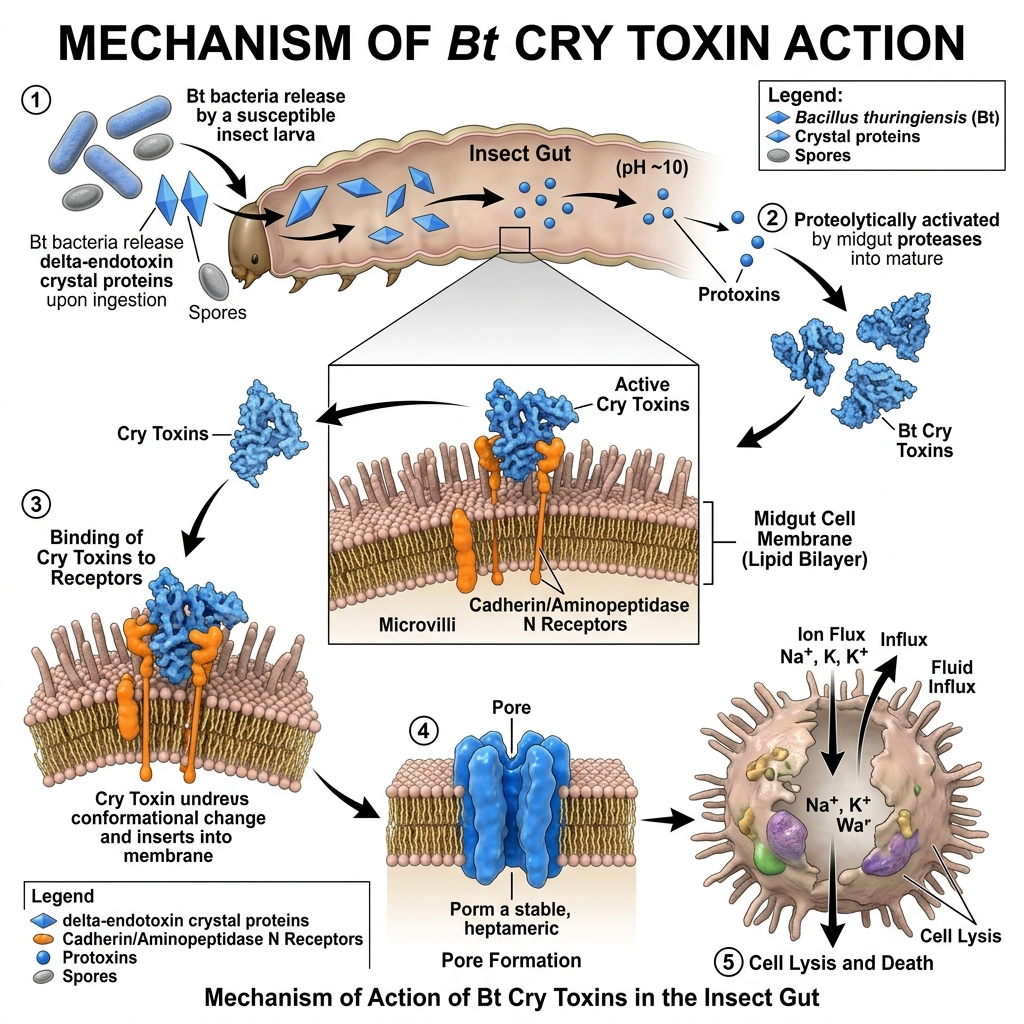
\includegraphics[width=0.85\textwidth]{assets/ch05_bt_mechanism.png}
    \caption{การจำลองภาพ 3D ขยายแสดงกลไกการทำลายของผลึกสารพิษเดลตา-เอนโดท็อกซิน (Delta-endotoxin: Cry toxin) ของแบคทีเรีย Bt ในลำไส้ส่วนกลางของหนอนแมลงศัตรูพืช แสดงขั้นตอนการหลอมละลายผลึกในสภาวะด่างจัด การตัดแต่งโมเลกุลด้วยเอนไซม์โปรติเอส การเข้าจับกับตัวรับ Cadherin และการรวมกลุ่มแทรกตัวสร้างรูรั่วทะลวงเยื่อหุ้มเซลล์ (Pore Formation) จนเซลล์แตกสลาย}
    \label{fig:ch05_bt_mechanism}
\end{figure}

\section*{วัตถุประสงค์การเรียนรู้ประจำบท}
เมื่อศึกษาบทเรียนนี้จบแล้ว นักศึกษาสามารถ:
\begin{enumerate}
    \item อธิบายโครงสร้างระดับ 3 มิติ และลำดับการออกฤทธิ์ทางชีวเคมีของโปรตีนสารพิษ Cry และ Cyt จาก \organism{Bacillus thuringiensis}
    \item วิเคราะห์กลไกปฏิปักษ์ 4 ด้านของเชื้อรา \organism{Trichoderma} spp. (Mycoparasitism, Antibiosis, Competition, Induced Resistance)
    \item อธิบายโครงสร้างและบทบาทของสารไลโปเปปไทด์วงแหวน (Surfactin, Iturin, Fengycin) ที่ผลิตโดย \organism{Bacillus subtilis}
    \item ลำดับขั้นตอนการเข้าทำลายแมลงศัตรูพืชของเชื้อรา \organism{Beauveria} และ \organism{Metarhizium} และสารพิษ mycotoxins ที่เกี่ยวข้อง
    \item คำนวณค่าร้อยละการยับยั้งการเจริญเติบโตของเส้นใยรา (PIRG) และคำนวณค่าความเข้มข้นที่ทำให้แมลงตายร้อยละ 50 ($LC_{50}$) จากข้อมูลชีววิเคราะห์
\end{enumerate}

\section{ชีวเคมีระดับโมเลกุลของสารพิษ Bacillus thuringiensis (Bt)}

\organism{Bacillus thuringiensis} (Bt) เป็นแบคทีเรียแกรมบวกรูปท่อนที่สร้างสปอร์ (Endospore-forming) อยู่ในดิน เมื่อเข้าสู่ระยะการสร้างสปอร์ (Sporulation) ยีนบนพลาสมิดจะสั่งการให้สังเคราะห์ผลึกโปรตีนข้างสปอร์ (Parasporal body) เรียกว่า \textbf{เดลตา-เอนโดท็อกซิน ($\delta$-endotoxins)} ซึ่งประกอบด้วยสองตระกูลหลักคือ \textbf{Cry toxins\index{สารพิษ Cry (Cry toxins)}} (Crystal proteins) และ \textbf{Cyt toxins\index{สารพิษ Cyt (Cytolytic toxins)}} (Cytolytic proteins)

\subsection{1. โครงสร้าง 3 มิติของโปรตีน Cry}
โมเลกุลโปรตีน Cry ที่ออกฤทธิ์ประกอบด้วย 3 โดเมนโครงสร้างหลัก (Three-domain Cry toxins):
\begin{itemize}
    \item \textbf{Domain I (N-terminal domain):} ประกอบด้วยกลุ่มเกลียวแอลฟา 7 สาย ($\alpha$-helices) ล้อมรอบเกลียวกลาง $\alpha$-5 โดเมนนี้ทำหน้าที่เป็น \textbf{หัวเจาะทะลวงเยื่อหุ้มเซลล์และสร้างรูรั่ว (Pore formation)}
    \item \textbf{Domain II (Middle domain):} ประกอบด้วยแผ่นเบตา 3 ชุด ($\beta$-sheets) บิดเป็นรูปทรงคล้ายเสานิ้วมือ โดเมนนี้มีความแปรผันทางพันธุกรรมสูง ทำหน้าที่เป็น \textbf{ตัวจับจำเพาะกับตัวรับบนผิวเซลล์ลำไส้แมลง (Receptor binding)}
    \item \textbf{Domain III (C-terminal domain):} เป็นโครงสร้างเบตา-แซนด์วิช ($\beta$-sandwich jellyroll) ทำหน้าที่รักษาเสถียรภาพของโมเลกุล ป้องกันการย่อยสลายก่อนเวลาอันควร และช่วยในการจับกับตัวรับร่วม
\end{itemize}

\subsection{2. กลไกการเกิดพิษต่อระบบทางเดินอาหารแมลง (Colloid-Osmotic Lysis)}
กระบวนการทำลายเยื่อบุผิวลำไส้ของหนอนศัตรูพืชดำเนินไปอย่างเป็นลำดับขั้น:
\begin{enumerate}
    \item \textbf{การหลอมละลายผลึก (Solubilization):} แมลงกินผลึกโปรตีน Bt เข้าไป เมื่อถึงลำไส้ส่วนกลาง (Midgut) ซึ่งมีสภาวะด่างจัด ($\text{pH } 9.0 - 11.5$) ผลึกโปรตีนที่ไม่ละลายน้ำจะแตกตัวละลายกลายเป็นโปรท็อกซินขนาดโมเลกุลประมาณ $130 - 140\text{ kDa}$
    \item \textbf{การตัดแต่งโปรตีนด้วยเอนไซม์ (Proteolytic Activation):} เอนไซม์กลุ่มเซอรีนโปรติเอส (Trypsin- and chymotrypsin-like proteases) ในน้ำย่อยของหนอนจะตัดชิ้นส่วนปลาย N-terminus (ประมาณ 28 กรดอะมิโน) และปลาย C-terminus ทิ้ง ทำให้โมเลกุลเล็กลงเหลือขนาด $60 - 65\text{ kDa}$ ซึ่งเป็นรูปแอคทีฟท็อกซิน (Active toxin)
    \item \textbf{การเข้าจับกับตัวรับจำเพาะ (Receptor Binding):} โมเลกุลสารพิษเข้าจับกับตัวรับ Cadherin-like receptors (CAD) บนผิวไมโครวิลไล (Microvilli) ของเซลล์บุผนังลำไส้ การจับนี้เหนี่ยวนำให้เอนไซม์ตัดชิ้นส่วนเกลียว $\alpha$-1 ออก นำไปสู่การรวมตัวของโปรตีนเป็นโมเลกุลกลุ่มสี่ (Tetrameric oligomer) หรือ ``Pre-pore structure''
    \item \textbf{การแทรกทะลวงสร้างรู (Membrane Insertion and Pore Formation):} โครงสร้างพรีพอร์เข้าจับกับตัวรับร่วมประเภท GPI-anchored proteins เช่น Aminopeptidase N (APN) และ Alkaline Phosphatase (ALP) จากนั้นแทรกตัวฝังลงในชั้นไขมันลิพิดไบเลเยอร์ ทำให้เกิดรูรั่วขนาดเส้นผ่านศูนย์กลาง $1 - 2\text{ นาโนเมตร}$
    \item \textbf{เซลล์แตกสลายและการติดเชื้อในกระแสเลือด (Colloid-Osmotic Lysis \& Septicemia):} รูรั่วบนเยื่อหุ้มเซลล์ทำให้สูญเสียศักย์ไฟฟ้า ไอออน $K^+$ และน้ำไหลทะลักเข้าสู่เซลล์อย่างควบคุมไม่ได้ เซลล์บุลำไส้บวมเป่งและแตกสลาย หนอนหยุดกินอาหารภายในไม่กี่ชั่วโมง ผนังลำไส้ทะลุ ส่งผลให้แบคทีเรียและสปอร์ไหลทะลักเข้าสู่ช่องลำตัว (Hemolymph) เกิดภาวะโลหิตเป็นพิษและหนอนตายภายใน $24 - 72\text{ ชั่วโมง}$
\end{enumerate}

\section{เชื้อรา Trichoderma: อัศวินแห่งชีวภัณฑ์ปฏิปักษ์}

เชื้อราสกุล \organism{Trichoderma}\index{Trichoderma harzianum@\textit{Trichoderma harzianum}} (เช่น \organism{Trichoderma harzianum}, \organism{T. asperellum}, และ \organism{T. viride}) เป็นเชื้อราปฏิปักษ์ที่มีประสิทธิภาพสูงสุดในการควบคุมเชื้อราก่อโรคพืชในดิน โดยมีกลไกการออกฤทธิ์ประสานกัน 4 ประการ:

\subsection{1. การเป็นปรสิตต่อเชื้อราอื่น (Mycoparasitism)}
กระบวนการไมโคพาราซิติซึม\index{Mycoparasitism (ภาวะปรสิตของรา)}เป็นลำดับขั้นชีวโมเลกุลที่แม่นยำ:
\begin{itemize}
    \item \textbf{การตรวจจับและเจริญเข้าหา (Chemotropism):} \organism{Trichoderma} รับรู้สารเคมีที่หลั่งจากเส้นใยเชื้อราเหยื่อ แล้วเจริญเติบโตมุ่งตรงเข้าหา
    \item \textbf{การรับรู้และเข้าเกาะ (Recognition and Binding):} โมเลกุลเลกติน (Lectins) บนผิวเซลล์เหยื่อจับกับตัวรับบนผิว \organism{Trichoderma} จากนั้นเส้นใยปฏิปักษ์จะพันรัด (Coiling) รอบเส้นใยของเชื้อราก่อโรคอย่างแน่นหนา
    \item \textbf{การหลั่งเอนไซม์ย่อยผนังเซลล์รา (CWDEs):} \organism{Trichoderma} หลั่งกลุ่มเอนไซม์ย่อยสลายผนังเซลล์ชีวโมเลกุล ได้แก่:
    \begin{itemize}
        \item \textbf{Chitinases:\index{เอนไซม์ไคทิเนส (Chitinase)}} เช่น Endo-chitinase (EC 3.2.1.14) สุ่มตัดพันธะ $\beta$-1,4 ภายในสายพอลิเมอร์ไคติน และ Exo-chitinase / $\beta$-N-acetylglucosaminidase (EC 3.2.1.52) ตัดน้ำตาลจากปลายสาย
        \item \textbf{$\beta$-1,3-glucanases:\index{เอนไซม์กลูคาเนส ($\beta$-Glucanase)}} สลายสายโซ่กลูแคนที่ทำหน้าที่เป็นโครงร่างหลักของผนังเซลล์รา
        \item \textbf{Proteases:} ย่อยสลายโครงสร้างโปรตีนที่แทรกอยู่ในผนังเซลล์
    \end{itemize}
\end{itemize}
เมื่อผนังเซลล์เชื้อราก่อโรคถูกเจาะเป็นรู \organism{Trichoderma} จะสร้างโครงสร้างคล้ายแอพเพรสโซเรียมแทงเข้าไปดูดกินไซโตพลาสซึมของเหยื่อจนเส้นใยยุบตัวและสลายไป

\begin{figure}[ht]
\centering
\begin{tikzpicture}[node distance=1.4cm, auto,
    stage/.style={rectangle, draw=agriGreen, fill=agriGrayBox, text width=11.5cm, rounded corners, minimum height=0.9cm, align=left, font=\small},
    arrow/.style={thick, ->, >=stealth, color=agriGreen}]
    
    \node [stage] (s1) {\textbf{ระยะที่ 1: Chemotropic Growth} รับรู้สารเคมีที่หลั่งจากเชื้อราเหยื่อ เจริญเติบโตมุ่งตรงเข้าหา};
    \node [stage, below of=s1] (s2) {\textbf{ระยะที่ 2: Recognition \& Coiling} โมเลกุล Lectins ผิวเซลล์จับจำเพาะ เส้นใยไตรโคเดอร์มาพันรัดรอบเส้นใยเหยื่อ};
    \node [stage, below of=s2] (s3) {\textbf{ระยะที่ 3: Secretion of CWDEs} หลั่งเอนไซม์ Endo/Exo-Chitinase, $\beta$-1,3-glucanase และ Peptaibols};
    \node [stage, below of=s3] (s4) {\textbf{ระยะที่ 4: Lysis \& Penetration} เจาะทะลุผนังเซลล์ ดูดกินไซโตพลาสซึมจนเส้นใยเชื้อราก่อโรคยุบสลาย};
    
    \draw [arrow] (s1) -- (s2);
    \draw [arrow] (s2) -- (s3);
    \draw [arrow] (s3) -- (s4);
\end{tikzpicture}
\caption{ลำดับขั้นทางชีวโมเลกุลในกระบวนการ Mycoparasitism ของเชื้อราปฏิปักษ์ \organism{Trichoderma} ในการเข้าทำลายเส้นใยเชื้อราก่อโรคพืช}
\label{fig:trichoderma_mycoparasitism}
\end{figure}

\subsection{2. การสร้างสารปฏิชีวนะยับยั้งการเจริญ (Antibiosis)}
\organism{Trichoderma} สังเคราะห์สารทุติยภูมิที่มีฤทธิ์ต้านจุลชีพหลายตระกูล:
\begin{itemize}
    \item \textbf{Peptaibols:\index{Peptaibols}} เปปไทด์สายสั้น (15--20 กรดอะมิโน) ที่มีกรดอะมิโนแปลกอย่าง $\alpha$-aminoisobutyric acid (Aib) ทำหน้าที่แทรกตัวสร้างรูรั่วบนเยื่อหุ้มเซลล์ของเชื้อราก่อโรค ทำงานเสริมฤทธิ์ (Synergy) กับเอนไซม์ CWDEs
    \item \textbf{6-pentyl-$\alpha$-pyrone (6-PP):} สารระเหยที่มีกลิ่นหอมคล้ายมะพร้าว มีฤทธิ์ยับยั้งการงอกของสปอร์เชื้อราก่อโรคพืช เช่น \organism{Fusarium oxysporum} และ \organism{Botrytis cinerea}
    \item \textbf{Gliovirin และ Gliotoxin:} สารประกอบอีพิดิทิโอไดคีโทพิเพอราซีน (ETP) ที่ยับยั้งกระบวนการหายใจระดับเซลล์ของเชื้อก่อโรค
\end{itemize}

\subsection{3. การแย่งชิงสารอาหารและพื้นที่ (Competition for Nutrients and Space)}
\organism{Trichoderma} มีอัตราการเติบโตของเส้นใยที่เร็วกว่าเชื้อราก่อโรคพืชทั่วไป 2--3 เท่า สามารถครอบครองพื้นที่ผิวรากได้อย่างรวดเร็ว นอกจากนี้ยังสร้างสารไซเดอโรฟอร์จับไอออนเหล็ก ($Fe^{3+}$) ทำให้เชื้อก่อโรคขาดแคลนธาตุเหล็กในการดำรงชีพ

\section{สารปฏิชีวนะชีวภาพไลโปเปปไทด์ของแบคทีเรีย Bacillus subtilis}

แบคทีเรีย \organism{Bacillus subtilis} และ \organism{Bacillus velezensis} ได้รับการยอมรับในระดับสากลว่าเป็นโรงงานเคมีชีวภาพเคลื่อนที่ในดิน จุลินทรีย์กลุ่มนี้สังเคราะห์ \textbf{สารไลโปเปปไทด์วงแหวน (Cyclic Lipopeptides: CLPs)\index{สารประกอบไลโปเปปไทด์ (Lipopeptides)}} ผ่านเอนไซม์มัลติเอนไซม์นอนไรโบโซมอลเปปไทด์ซินเทเทส (Non-Ribosomal Peptide Synthetases: NRPSs) ซึ่งแบ่งออกเป็น 3 ตระกูลเด่น:

\begin{table}[ht]
\centering
\small
\setlength{\tabcolsep}{4pt}
\begin{tabular}{p{2.3cm}p{4.2cm}p{5.5cm}}
\toprule
\textbf{ตระกูลสารไลโปเปปไทด์} & \textbf{โครงสร้างโมเลกุลเด่น} & \textbf{กลไกการออกฤทธิ์ทางชีวภาพ} \\
\midrule
\textbf{Surfactin\index{Surfactin}} & เปปไทด์ 7 อะมิโน + สายกรดไขมัน $\beta$-hydroxy $C_{13}-C_{15}$ & สารลดแรงตึงผิวชีวภาพที่มีประสิทธิภาพสูงสุด แทรกตัวรบกวนชั้นลิพิดไบเลเยอร์ ทำให้เยื่อหุ้มเซลล์เสียสภาพ ละลายคราบไบโอฟิล์มของแบคทีเรียก่อโรค \\
\textbf{Iturin (Iturin A, Mycosubtilin)\index{Iturin}} & เปปไทด์ 7 อะมิโน + สายกรดไขมัน $\beta$-amino $C_{14}-C_{17}$ & มีฤทธิ์ต้านเชื้อราที่รุนแรงมาก เข้าจับกับสเตอรอล (Ergosterol) บนเยื่อหุ้มเซลล์รา เกิดเป็นรูรั่วขนาดเล็ก ทำให้เกิดการรั่วไหลของ $K^+$ \\
\textbf{Fengycin (Plipastatin)\index{Fengycin}} & เปปไทด์ 10 อะมิโน + สายกรดไขมัน $\beta$-hydroxy $C_{14}-C_{18}$ & มีความจำเพาะสูงต่อเชื้อราเส้นใย (Filamentous fungi) ทำลายเสถียรภาพเยื่อหุ้มเซลล์ราและกระตุ้นการตายของเซลล์รา \\
\bottomrule
\end{tabular}
\caption{ตารางเปรียบเทียบคุณลักษณะและกลไกของสารไลโปเปปไทด์วงแหวนหลักจาก \organism{Bacillus subtilis}}
\label{tab:bacillus_lipopeptides}
\end{table}

\section{เชื้อรากำจัดแมลงศัตรูพืช (Entomopathogenic Fungi)}

เชื้อรากลุ่มเอ็นโทโมพาโทเจนิก\index{เชื้อรากำจัดแมลง (Entomopathogenic Fungi)} เช่น \organism{Beauveria bassiana}\index{Beauveria bassiana@\textit{Beauveria bassiana}} (เชื้อราขาว) และ \organism{Metarhizium anisopliae}\index{Metarhizium anisopliae@\textit{Metarhizium anisopliae}} (เชื้อราเขียว) มีความโดดเด่นเหนือกว่าแบคทีเรีย Bt ตรงที่ \textbf{ไม่ต้องรอให้แมลงกินเข้าไป} แต่สามารถเจาะทะลุผนังลำตัว (Integument / Cuticle) ของแมลงได้โดยตรง

\subsection{1. กลไกการเจาะผ่านเกราะคิวทิเคิลของแมลง}
ผนังลำตัวแมลงประกอบด้วยโปรตีน ไคติน และไขแว็กซ์ที่ทนทานสูง เชื้อราอาศัยการทำงานประสานกันของเอนไซม์นอกเซลล์ 3 กลุ่ม:
\begin{enumerate}
    \item \textbf{Esterases and Lipases:} สลายชั้นแว็กซ์ด้านนอกสุด (Epicuticle)
    \item \textbf{Pr1 Proteases (Subtilisin-like proteases):} ย่อยสลายโครงข่ายโปรตีนที่ห่อหุ้มเส้นใยไคติน เป็นเอนไซม์ตัวชี้วัดความรุนแรงของเชื้อ
    \item \textbf{Endochitinases:} ย่อยเส้นใยไคติน ทำให้เข็มเจาะแทงทะลุเข้าสู่ช่องลำตัวแมลงได้สำเร็จ
\end{enumerate}

\subsection{2. การหลบหลีกภูมิคุ้มกันและการสร้างสารพิษในตัวแมลง}
เมื่อเข้าสู่ช่องฮีโมซีล (Hemocoel) เชื้อราจะเปลี่ยนรูปร่างจากเส้นใยเป็นเซลล์ยีสต์รูปไข่ (Blastospores) ที่ไม่มีชั้นผนังเซลล์ด้านนอก ทำให้เม็ดเลือดแมลง (Hemocytes) ไม่สามารถตรวจจับเพื่อสร้างแคปซูลห่อหุ้ม (Encapsulation) ได้ จากนั้นเชื้อจะหลั่งสารพิษ mycotoxins:
\begin{itemize}
    \item \textbf{Beauvericin (จาก \organism{Beauveria}):} ไอออนโนฟอร์วงแหวนที่เหนี่ยวนำให้ $Ca^{2+}$ ไหลทะลักเข้าเซลล์ รบกวนระบบประสาทและกล้ามเนื้อแมลง
    \item \textbf{Destruxins (จาก \organism{Metarhizium}):} ยับยั้งการทำงานของโปรตีน ATPase และยับยั้งการขับถ่ายของท่อมัลพิเกียน
\end{itemize}
เมื่อแมลงตาย เส้นใยจะแทงทะลุซากแมลงออกมาภายนอกและสร้างสปอร์คลุมซากแห้ง (Mummified insect) เป็นสีขาวฟูหรือสีเขียวเข้ม เรียกว่าโรคราขาว (White muscardine) และโรคราเขียว (Green muscardine) ตามลำดับ

\section{การคำนวณทางชีววิเคราะห์และการทดสอบประสิทธิภาพชีวภัณฑ์}

\subsection{1. ดัชนีการยับยั้งการเจริญของเส้นใยรา (PIRG)}
ในการทดสอบประสิทธิภาพของเชื้อราปฏิปักษ์ เช่น \organism{Trichoderma} ต่อเชื้อราก่อโรคในจานเพาะเชื้อด้วยเทคนิค Dual Culture Assay นิยมคำนวณ \textbf{เปอร์เซ็นต์การยับยั้งการเจริญเติบโตของรัศมีเส้นใย (Percent Inhibition of Radial Growth: PIRG)\index{ร้อยละการยับยั้งการเจริญ (PIRG)}}:

\begin{equation}
\text{PIRG} = \frac{R_1 - R_2}{R_1} \times 100
\end{equation}

เมื่อ $R_1$ คือรัศมีการเจริญของโคโลนีเชื้อราก่อโรคในจานควบคุม (มิลลิเมตร) และ $R_2$ คือรัศมีการเจริญของเชื้อราก่อโรคในจานทดสอบที่มีเชื้อปฏิปักษ์ (มิลลิเมตร)

\subsection{2. การวิเคราะห์โพรบิตและค่าความเข้มข้นกึ่งทำลาย (\texorpdfstring{$LC_{50}$}{LC50})}
การประเมินความเป็นพิษของสูตรตำรับ Bt หรือสปอร์เชื้อรากำจัดแมลง ใช้ค่า **$LC_{50}$ (Lethal Concentration 50)** ซึ่งหมายถึงความเข้มข้นของชีวภัณฑ์ที่ทำให้ประชากรแมลงทดลองตายร้อยละ 50 ภายในระยะเวลาที่กำหนด โดยแปลงอัตราร้อยละการตายเป็นหน่วย **Probit (Probability Unit)** เพื่อสร้างสมการเส้นตรง:

\begin{equation}
Y = a + b \log_{10}(C)
\end{equation}

เมื่อ $Y$ คือค่า Probit ของอัตราการตาย, $C$ คือความเข้มข้นของชีวภัณฑ์, $a$ คือจุดตัดแกน Y และ $b$ คือความชัน (Slope) ของกราฟ เมื่อคำนวณที่อัตราการตาย 50\% ($Y = 5.0$) จะได้ค่า $\log_{10}(LC_{50}) = (5.0 - a)/b$

\begin{worked}[ตัวอย่างที่ 5.1 การประเมินประสิทธิภาพของ \organism{Trichoderma} ต่อเชื้อราก่อโรครากเน่า]
นักศึกษาภาควิชาชีววิทยาทำการทดสอบ Dual Culture ระหว่าง \organism{Trichoderma harzianum} กับเชื้อราก่อโรครากเน่า \organism{Fusarium oxysporum} บนอาหารเลี้ยงเชื้อ PDA เป็นเวลา 7 วัน:
\begin{itemize}
    \item จานควบคุม (เลี้ยง \organism{F. oxysporum} เดี่ยว): รัศมีโคโลนี $R_1 = 42.5\text{ mm}$
    \item จานทดสอบ (เลี้ยงคู่กับ \organism{T. harzianum}): รัศมีโคโลนีของเชื้อก่อโรคเหลือ $R_2 = 14.0\text{ mm}$
\end{itemize}
จงคำนวณค่า PIRG และวิเคราะห์ระดับประสิทธิภาพตามเกณฑ์มาตรฐานชีววิธี

\textbf{วิธีทำ:}
$$\text{PIRG} = \frac{R_1 - R_2}{R_1} \times 100 = \frac{42.5 - 14.0}{42.5} \times 100 = \frac{28.5}{42.5} \times 100 \approx 67.06\%$$

\textbf{บทวิเคราะห์ผลลัพธ์:} ค่า PIRG เท่ากับ 67.06\% (สูงกว่าเกณฑ์มาตรฐาน 60\%) บ่งชี้ว่า \organism{Trichoderma harzianum} สายพันธุ์นี้มีศักยภาพปฏิปักษ์ระดับสูง (High Antagonistic Activity) โดยเกิดจากกลไกการเจริญแย่งชิงพื้นที่ร่วมกับการหลั่งสารต้านจุลชีพ 6-PP และเอนไซม์ย่อยไคติน ทำให้เชื้อราก่อโรคไม่สามารถแผ่ขยายโคโลนีได้ตามปกติ
\end{worked}

\begin{worked}[ตัวอย่างที่ 5.2 การหาค่า $LC_{50}$ ของชีวภัณฑ์ Bt ต่อหนอนกระทู้ข้าวโพดลายจุด]
จากการทดสอบป้อนใบข้าวโพดจุ่มสารแขวนลอยสปอร์ Bt ให้แก่หนอนกระทู้ข้าวโพดลายจุด (\organism{Spodoptera frugiperda}) วัยที่ 2 จำนวนความเข้มข้น 5 ระดับ เมื่อนำข้อมูลมาพล็อตความสัมพันธ์ระหว่าง Probit ($Y$) กับ $\log_{10}(\text{Concentration})$ ได้สมการถดถอยเชิงเส้น:
$$Y = 1.45 + 1.82 \log_{10}(C)$$
โดยที่ $C$ มีหน่วยเป็น $\mu\text{g/mL}$ จงคำนวณหาค่า $LC_{50}$ ของชีวภัณฑ์ Bt นี้

\textbf{วิธีทำ:}
ที่อัตราการตาย 50\% ค่า Probit มาตรฐานสากลคือ $Y = 5.0$
แทนค่า $Y = 5.0$ ลงในสมการ:
$$5.0 = 1.45 + 1.82 \log_{10}(LC_{50})$$
$$1.82 \log_{10}(LC_{50}) = 5.0 - 1.45 = 3.55$$
$$\log_{10}(LC_{50}) = \frac{3.55}{1.82} \approx 1.9505$$
$$LC_{50} = 10^{1.9505} \approx 89.23 \mu\text{g/mL}$$

\textbf{บทวิเคราะห์ผลลัพธ์:} ความเข้มข้นสารพิษ Bt เพียง $89.23 \mu\text{g/mL}$ สามารถกำจัดหนอนกระทู้ได้ถึงกึ่งหนึ่งของประชากรทดสอบ ถือเป็นชีวภัณฑ์ที่มีความไวสูง (High Potency) เหมาะสำหรับนำไปตั้งตำรับเพื่อใช้พ่นระงับการระบาดในแปลงเกษตรอินทรีย์
\end{worked}

% [RESEARCH-UPDATE-2026-10]
\section{ความก้าวหน้างานวิจัยล่าสุดด้านการควบคุมโรคพืชโดยชีววิธี}

งานทบทวนวรรณกรรมระดับนานาชาติในปี ค.ศ. 2023–2025 โดย Tyśkiewicz และคณะ \cite{pmid36771517} ชี้ให้เห็นว่าสายพันธุ์ \organism{Trichoderma} ที่คัดแยกจากพื้นที่เกษตรเขตร้อนมียีนควบคุมการสร้างสารทุติยภูมิกลุ่มเปปไทบอิล (Peptaibols) หลากหลายกว่าสายพันธุ์เขตหนาว ส่งผลให้มีความทนทานต่อสภาวะอุณหภูมิสูงในแปลงปลูกได้ดีกว่า

ในขณะเดียวกัน งานวิจัยของ Ongena และคณะ \cite{pmid37837627} ได้ยืนยันว่าการใช้แบคทีเรียกลุ่ม \organism{Bacillus} สายพันธุ์ที่ผลิตไลโปเปปไทด์ Surfactin และ Fengycin ร่วมกัน จะก่อให้เกิดผลเสริมฤทธิ์แบบทวีคูณ (Synergistic effect) โดย Surfactin จะไปเปิดช่องว่างบนเยื่อหุ้มเซลล์รา ทำให้ Fengycin สามารถแทรกซึมเข้าทำลายโครงสร้างภายในเซลล์ราก่อโรคได้อย่างรวดเร็ว

\begin{insight}[ประเด็นวิเคราะห์เชิงวิชาการ]
เกษตรกรบางรายพบว่าการฉีดพ่นเชื้อรากำจัดแมลง \organism{Beauveria bassiana} ในช่วงเที่ยงวันแดดจัดให้ผลการควบคุมต่ำมาก จงวิเคราะห์ปัจจัยทางฟิสิกส์และสิ่งแวดล้อมที่มีผลต่อความมีชีวิตของสปอร์ พร้อมเสนอแนวทางการแก้ปัญหาในระดับสูตรตำรับ (Formulation)
\end{insight}

\section*{สรุปประจำบท}

การควบคุมศัตรูพืชโดยชีววิธีด้วยจุลินทรีย์ปฏิปักษ์เป็นเครื่องมือทรงประสิทธิภาพในการลดการพึ่งพาสารเคมีสังเคราะห์ แบคทีเรีย \organism{Bacillus thuringiensis} อาศัยโครงสร้างผลึกโปรตีน Cry และ Cyt ที่เจาะทำลายเซลล์เยื่อบุทางเดินอาหารของแมลงอย่างจำเพาะเจาะจง เชื้อรา \organism{Trichoderma} ใช้การทำงานร่วมกันระหว่างการพันรัดไมโคพาราซิติซึม เอนไซม์ย่อยผนังเซลล์ (ไคติเนสและเบตา-กลูคาเนส) และสารปฏิชีวนะเปปไทบอิล ขณะที่ \organism{Bacillus subtilis} ผลิตไลโปเปปไทด์วงแหวน (Surfactin, Iturin, Fengycin) ยับยั้งเชื้อราก่อโรคอย่างกว้างขวาง และเชื้อรากำจัดแมลง (\organism{Beauveria} และ \organism{Metarhizium}) มีความสามารถพิเศษในการเจาะทะลุเกราะไคตินของแมลงได้โดยตรง การประเมินประสิทธิภาพในห้องปฏิบัติการผ่านค่า PIRG และ $LC_{50}$ ช่วยให้นักวิจัยสามารถคัดเลือกสายพันธุ์และตั้งสูตรตำรับชีวภัณฑ์ที่มีความเสถียรและออกฤทธิ์สูงสุดในแปลงเกษตรกรรมจริง

\subsection*{คำถามท้ายบทและการวิเคราะห์}

\noindent \textbf{ระดับที่ 1: ความรู้และความเข้าใจเชิงทฤษฎี (Knowledge \& Comprehension)}
\begin{enumerate}
    \item อธิบายหน้าที่ของแต่ละโดเมน (Domain I, II, III) ในโมเลกุลผลึกโปรตีน Cry ของแบคทีเรีย \organism{Bacillus thuringiensis}
    \item เหตุใดผลึกโปรตีน Bt จึงไม่เป็นพิษต่อกระเพาะอาหารของมนุษย์และสัตว์มีกระดูกสันหลัง? จงอธิบายโดยอ้างอิงสภาวะทางเคมีและตัวรับในทางเดินอาหาร
    \item สรุปขั้นตอนระดับโมเลกุลในปรากฏการณ์ Mycoparasitism ของเชื้อรา \organism{Trichoderma} ที่มีต่อเชื้อราก่อโรคพืช
    \item เอนไซม์ Endo-chitinase และ Exo-chitinase แตกต่างกันอย่างไรในแง่ของตำแหน่งการตัดพันธะและผลิตภัณฑ์ที่ได้จากการย่อยสลายไคติน?
\end{enumerate}

\noindent \textbf{ระดับที่ 2: การวิเคราะห์และการคำนวณเชิงปริมาณ (Quantitative Analysis \& Calculation)}
\begin{enumerate}[resume]
    \item สารประกอบ Cyclic Lipopeptides ทั้ง 3 กลุ่มของ \organism{Bacillus subtilis} (Surfactin, Iturin, Fengycin) มีกลไกการออกฤทธิ์ทางชีวภาพแตกต่างกันอย่างไร?
    \item ในการทดสอบ Dual culture assay จานควบคุมมีรัศมีโคโลนีของเชื้อราก่อโรค $R_1 = 38.0\text{ mm}$ และจานที่มีเชื้อราปฏิปักษ์มีรัศมี $R_2 = 9.5\text{ mm}$ จงคำนวณหาค่า PIRG และแปลความหมายผลลัพธ์
    \item หากสมการ Probit ของชีวภัณฑ์ Bt ชนิดหนึ่งต่อหนอนใยผักคือ $Y = 2.10 + 1.60 \log_{10}(C)$ จงคำนวณหาค่า $LC_{50}$ ในหน่วย $\mu\text{g/mL}$
\end{enumerate}

\noindent \textbf{ระดับที่ 3: การสังเคราะห์และการแก้ปัญหาในแปลงจริง (Application \& Real-World Synthesis)}
\begin{enumerate}[resume]
    \item เชื้อรากำจัดแมลง \organism{Beauveria bassiana} ใช้เอนไซม์ชนิดใดบ้างในการเจาะทะลุชั้นคิวทิเคิลของแมลง และสารพิษ Beauvericin มีผลอย่างไรต่อเซลล์แมลง?
    \item เพราะเหตุใดการผสมสารลดแรงตึงผิวและสารป้องกันรังสีอัลตราไวโอเลต (UV Protectants) ในสูตรตำรับสปอร์ชีวภัณฑ์จึงช่วยเพิ่มประสิทธิภาพการออกฤทธิ์ในแปลงเกษตรได้อย่างมีนัยสำคัญ?
    \item ออกแบบแผนการจัดการศัตรูพืชแบบผสมผสาน (IPM) สำหรับสวนผลไม้ที่ต้องการลดการใช้สารเคมี โดยบูรณาการการใช้ Bt, \organism{Trichoderma} และ \organism{Beauveria} อย่างเป็นระบบตามระยะการเจริญเติบโตของพืช
\end{enumerate}

\chapter{วิศวกรรมการหมักและเทคโนโลยีการผลิตปุ๋ยชีวภาพระดับอุตสาหกรรม}
\label{ch:biofertilizers}

\begin{keyconcept}[แนวคิดสำคัญของบทที่ 6]
ปุ๋ยชีวภาพ (Biofertilizers)\index{ปุ๋ยชีวภาพ (Biofertilizers)} คือชีวภัณฑ์ที่บรรจุเซลล์จุลินทรีย์มีชีวิตที่มีความสามารถเฉพาะเจาะจงในการตรึงไนโตรเจน การละลายฟอสฟอรัสและโพแทสเซียม หรือการกระตุ้นการดูดซึมธาตุอาหารของรากพืช การขยายขนาดการผลิตจากระดับห้องปฏิบัติการสู่ระดับอุตสาหกรรมจำเป็นต้องอาศัยศาสตร์ด้าน \textbf{วิศวกรรมการหมัก (Fermentation Engineering)\index{วิศวกรรมการหมัก (Fermentation Engineering)}} การควบคุมจลนศาสตร์การเพาะเลี้ยงแบบกะ (Batch) และกะกึ่งต่อเนื่อง (Fed-batch) การถ่ายโอนมวลออกซิเจน ($k_L a$)\index{สัมประสิทธิ์การถ่ายโอนออกซิเจน ($k_L a$)}\index{Oxygen transfer coefficient ($k_L a$)} ตลอดจนเทคโนโลยีการห่อหุ้มเซลล์ (Microencapsulation)\index{การห่อหุ้มเซลล์ระดับไมโคร (Microencapsulation)} ด้วยวัสดุพาหะชีวภาพ เช่น ถ่านไบโอชาร์และโซเดียมอัลจิเนต เพื่อรักษาความมีชีวิตของเซลล์ตามเกณฑ์มาตรฐาน พ.ร.บ. ปุ๋ย กรมวิชาการเกษตร\index{พ.ร.บ. ปุ๋ย กรมวิชาการเกษตร}
\end{keyconcept}

\begin{figure}[ht]
    \centering
    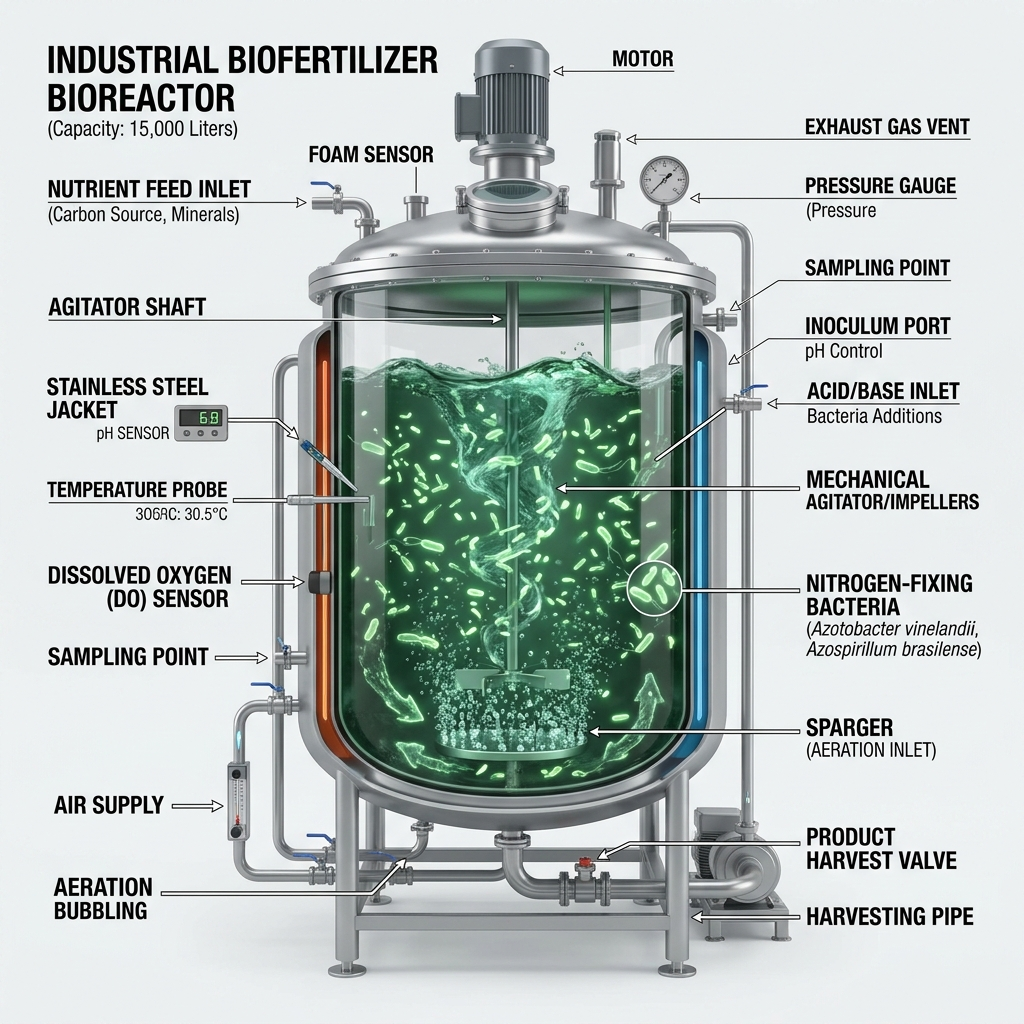
\includegraphics[width=0.85\textwidth]{assets/ch06_biofertilizer_fermentation.png}
    \caption{การจำลอง 3D ของเครื่องปฏิกรณ์ชีวภาพกวนสมบูรณ์ (Stirred-Tank Bioreactor) ขนาดกึ่งอุตสาหกรรม แสดงระบบจ่ายอากาศอัด (Sparger) ใบพัดกวนแบบ Rushton turbine เซนเซอร์วัดออกซิเจนละลายน้ำ (DO) และหัววัดกรด-ด่าง (pH) สำหรับการเพาะเลี้ยงแบคทีเรียปุ๋ยชีวภาพความหนาแน่นสูง}
    \label{fig:ch06_biofertilizer_fermentation}
\end{figure}

\section*{วัตถุประสงค์การเรียนรู้ประจำบท}
เมื่อศึกษาบทเรียนนี้จบแล้ว นักศึกษาสามารถ:
\begin{enumerate}
    \item จำแนกชนิดของปุ๋ยชีวภาพตามหน้าที่ทางชีวภาพและกลไกการปลดปล่อยธาตุอาหาร
    \item วิเคราะห์หลักการวิศวกรรมชีวภาพในการเพาะเลี้ยงเซลล์ความหนาแน่นสูง และการวัดสัมประสิทธิ์การถ่ายโอนมวลออกซิเจน ($k_L a$)
    \item เปรียบเทียบจลนศาสตร์การเพาะเลี้ยงแบบกะ (Batch) แบบกะกึ่งต่อเนื่อง (Fed-batch) และแบบต่อเนื่อง (Continuous)
    \item อธิบายเทคโนโลยีการตรึงเซลล์และการห่อหุ้มเซลล์ (Microencapsulation) ด้วยโซเดียมอัลจิเนตและวัสดุพาหะถ่านชีวภาพ (Biochar)
    \item ประเมินคุณภาพปุ๋ยชีวภาพตามเกณฑ์มาตรฐานกฎหมาย พ.ร.บ. ปุ๋ยของกรมวิชาการเกษตร และคำนวณปริมาณเซลล์มีชีวิต (CFU)
\end{enumerate}

\section{การจัดหมวดหมู่และกลไกสรีรวิทยาของปุ๋ยชีวภาพ}

ปุ๋ยชีวภาพจัดจำแนกตามคุณสมบัติการปลดปล่อยธาตุอาหารแก่พืชออกเป็น 4 กลุ่มหลัก:

\subsection{1. ปุ๋ยชีวภาพตรึงไนโตรเจน (Nitrogen-Fixing Biofertilizers)}
\begin{itemize}
    \item \textbf{กลุ่มพึ่งพาอาศัยในปมราก (Symbiotic):} แบคทีเรียสกุล \organism{Rhizobium}\index{Rhizobium@\textit{Rhizobium}}, \organism{Bradyrhizobium}\index{Bradyrhizobium@\textit{Bradyrhizobium}}, และ \organism{Sinorhizobium} สำหรับพืชตระกูลถั่ว สามารถตรึงไนโตรเจนได้สูงถึง $100 - 300\text{ kg N/ha/ปี}$
    \item \textbf{กลุ่มอยู่ร่วมกันแบบพึ่งพาภายนอก (Associative Symbiosis):} แบคทีเรียสกุล \organism{Azospirillum}\index{Azospirillum brasilense@\textit{Azospirillum brasilense}} (เช่น \organism{A. brasilense}) อาศัยบริเวณผิวรากและช่องว่างระหว่างเซลล์คอร์เทกซ์ของพืชตระกูลหญ้า ข้าว ข้าวโพด และอ้อย ตรึงไนโตรเจนได้ $20 - 50\text{ kg N/ha/ปี}$ พร้อมหลั่งฮอร์โมน IAA
    \item \textbf{กลุ่มดำรงชีวิตอิสระในดิน (Free-Living):} แบคทีเรียสกุล \organism{Azotobacter}\index{Azotobacter chroococcum@\textit{Azotobacter chroococcum}} (เช่น \organism{A. chroococcum}) และ \organism{Beijerinckia} ตรึงไนโตรเจนในสภาวะมีออกซิเจนโดยอาศัยกลไก Respiratory Protection
    \item \textbf{กลุ่มไซยาโนแบคทีเรีย (Cyanobacteria):} \organism{Anabaena azollae}\index{Anabaena azollae@\textit{Anabaena azollae}} ที่อาศัยในโพรงใบของแหนแดง (\organism{Azolla}) นิยมปล่อยลงในนาข้าวเพื่อเป็นปุ๋ยพืชสดไนโตรเจนสูง
\end{itemize}

\subsection{2. ปุ๋ยชีวภาพละลายฟอสฟอรัสและช่วยดูดซึม (Phosphate Biofertilizers)}
\begin{itemize}
    \item \textbf{แบคทีเรียและราละลายฟอสเฟต (Phosphate-Solubilizing Microorganisms: PSM):\index{แบคทีเรียละลายฟอสเฟต (PSB)}} เช่น \organism{Bacillus megaterium}\index{Bacillus megaterium@\textit{Bacillus megaterium}}, \organism{Pseudomonas putida}\index{Pseudomonas putida@\textit{Pseudomonas putida}}, และ \organism{Aspergillus niger} หลั่งกรดอินทรีย์โมเลกุลต่ำ (Citric acid, Gluconic acid, Oxalic acid) เพื่อคีเลตไอออน $Ca^{2+}, Fe^{3+}, Al^{3+}$ ปลดปล่อยออร์โทฟอสเฟตอิสระสู่สารละลายดิน
    \item \textbf{เชื้อราอาร์บัสคูลาร์ไมคอร์ไรซา (AMF):} เช่น \organism{Rhizophagus irregularis} เส้นใยราทำหน้าที่เป็นระบบรากเทียม (Extraradical mycelium) ดูดซับฟอสเฟตที่อยู่ห่างไกลส่งผ่านเข้าสู่รากพืชทางโครงสร้าง Arbuscules
\end{itemize}

\subsection{3. ปุ๋ยชีวภาพละลายโพแทสเซียมและซิลิเกต (Potassium \& Silicate Biofertilizers)}
แบคทีเรียสกุล \organism{Frateuria aurantia}\index{Frateuria aurantia@\textit{Frateuria aurantia}} และ \organism{Bacillus mucilaginosus} สามารถสร้างกรดอินทรีย์และสารเมือกพอลิแซ็กคาไรด์เข้าทำลายโครงสร้างผลึกแร่เฟลด์สปาร์ (Feldspar) และไมกา (Mica) ปลดปล่อยโพแทสเซียมไอออน ($K^+$) และกรดมอโนซิลิซิก ($H_4SiO_4$) ซึ่งช่วยเสริมความแข็งแรงของผนังเซลล์พืช

\section{วิศวกรรมการหมักและการเพาะเลี้ยงเซลล์ความหนาแน่นสูง}

การผลิตปุ๋ยชีวภาพเชิงพาณิชย์อาศัยเครื่องปฏิกรณ์ชีวภาพแบบถังกวนสมบูรณ์ (Stirred-Tank Bioreactor: STR) ซึ่งต้องควบคุมตัวแปรทางชีวเคมีและวิศวกรรมอย่างเข้มงวด:

\subsection{1. รูปแบบการเดินระบบการเพาะเลี้ยง (Modes of Fermentation)}
\begin{enumerate}
    \item \textbf{การเพาะเลี้ยงแบบกะ (Batch Culture):\index{การเพาะเลี้ยงแบบกะ (Batch Culture)}} บรรจุสารอาหารทั้งหมดลงในถัง ปิดฝา นึ่งฆ่าเชื้อ แล้วฉีดกล้าเชื้อ การเติบโตจะเป็นไปตามวัฏจักร Lag $\rightarrow$ Exponential $\rightarrow$ Stationary $\rightarrow$ Death phase ข้อเสียคือความเข้มข้นของเซลล์สุดท้ายถูกจำกัดด้วยสารอาหารที่หมดลงหรือการสะสมของของเสีย
    \item \textbf{การเพาะเลี้ยงแบบกะกึ่งต่อเนื่อง (Fed-batch Culture):\index{การเพาะเลี้ยงแบบกะกึ่งต่อเนื่อง (Fed-batch Culture)}} เป็นวิธีที่นิยมที่สุดในการผลิตปุ๋ยชีวภาพเกรดอุตสาหกรรม โดยเริ่มเดินระบบแบบกะปริมาตรเริ่มต้น $40 - 50\%$ เมื่อสารอาหารจำเพาะ (เช่น กลูโคสหรือกลีเซอรอล) ใกล้หมด จึงเริ่มป้อนสารอาหารเข้มข้นอย่างต่อเนื่องด้วยอัตราที่สอดคล้องกับอัตราการกินของเซลล์ ทำให้สามารถเพิ่มความหนาแน่นของเซลล์ (High Cell Density Cultivation)\index{การเพาะเลี้ยงเซลล์ความหนาแน่นสูง (HCDC)} ได้เกินกว่า $10^{10}\text{ CFU/mL}$ โดยไม่เกิดปรากฏการณ์ยับยั้งจากความเข้มข้นสารอาหารสูง (Substrate Inhibition)
    \item \textbf{การเพาะเลี้ยงแบบต่อเนื่อง (Continuous Culture / Chemostat):\index{การเพาะเลี้ยงแบบต่อเนื่อง (Continuous Culture)}} ป้อนสารอาหารสดเข้าและดูดน้ำหมักออกด้วยอัตราการเจือจาง ($D$) เท่ากับอัตราการเจริญจำเพาะ ($\mu$) มักใช้ในงานวิจัยสรีรวิทยามากกว่าการผลิตเชิงพาณิชย์เนื่องจากเสี่ยงต่อการปนเปื้อน
\end{enumerate}

\subsection{2. จลนศาสตร์การถ่ายโอนมวลออกซิเจน (\texorpdfstring{$k_L a$}{kLa})}
สำหรับจุลินทรีย์ที่ต้องการออกซิเจน (Aerobes) เช่น \organism{Azotobacter} และ \organism{Bacillus} อัตราการละลายของก๊าซออกซิเจนจากฟองอากาศสู่น้ำหมักมักเป็นขั้นตอนจำกัดความเร็ว (Rate-limiting step) สมดุลมวลของออกซิเจนละลายน้ำ (Dissolved Oxygen: DO) อธิบายได้ด้วยสมการ:

\begin{equation}
\frac{dC_L}{dt} = \text{OTR} - \text{OUR} = k_L a (C^* - C_L) - q_{O_2} X
\end{equation}

เมื่อ:
\begin{itemize}
    \item $C_L$ คือความเข้มข้นของออกซิเจนละลายน้ำในถังหมัก ($\text{mg/L}$ หรือ $\text{mmol/L}$)
    \item $C^*$ คือความเข้มข้นอิ่มตัวของออกซิเจนละลายน้ำ ณ อุณหภูมิและความดันนั้น ($\text{mg/L}$)
    \item $k_L a$ คือสัมประสิทธิ์รวมการถ่ายโอนมวลออกซิเจนตามปริมาตร (Volumetric Oxygen Transfer Coefficient, $\text{hr}^{-1}$ หรือ $\text{s}^{-1}$)
    \item $q_{O_2}$ คืออัตราการใช้ออกซิเจนจำเพาะของเซลล์ ($\text{mg } O_2/\text{g cell}\cdot\text{hr}$)
    \item $X$ คือความเข้มข้นของชีวมวลจุลินทรีย์ ($\text{g/L}$)
\end{itemize}

\section{เทคโนโลยีสูตรตำรับ วัสดุพาหะ และการห่อหุ้มเซลล์ (Microencapsulation)}

เพื่อให้เซลล์จุลินทรีย์ในปุ๋ยชีวภาพมีชีวิตรอดได้ยาวนานระหว่างการขนส่งและการเก็บรักษาในคลังสินค้า จึงมีการพัฒนาสูตรตำรับ 3 รูปแบบหลัก:\index{การห่อหุ้มเซลล์ระดับไมโคร (Microencapsulation)}

\subsection{1. สูตรผงพาหะแข็ง (Carrier-Based Powder Formulation)}
น้ำหมักจุลินทรีย์เข้มข้นจะถูกนำมาผสมกับวัสดุพาหะของแข็งที่ผ่านการนึ่งฆ่าเชื้อ (Sterilization) วัสดุพาหะที่ดีต้องมีความสามารถในการอุ้มน้ำสูง ($> 50\%$) มีรูพรุนระดับไมครอน มีค่า pH เป็นกลาง และไม่มีสารพิษ:
\begin{itemize}
    \item \textbf{ถ่านชีวภาพ (Biochar):\index{ถ่านชีวภาพ (Biochar)}} ผลิตจากการไพโรไลซิสวัสดุเหลือทิ้งทางการเกษตร (เช่น แกลบ กะลา มะพร้าว) โครงสร้างรูพรุนสูงช่วยเป็นที่หลบภัย (Refugia) ให้แก่จุลินทรีย์จากรังสี UV และจุลินทรีย์เจ้าถิ่นในดิน
    \item \textbf{พีทมอส (Peat Moss):} พาหะมาตรฐานดั้งเดิม มีสารอินทรีย์สูงแต่มีข้อจำกัดเรื่องต้นทุนและการทำลายสิ่งแวดล้อม
\end{itemize}

\subsection{2. สูตรน้ำเสถียรภาพสูง (Liquid Formulation)}
สูตรของเหลวบรรจุขวดที่เติมสารปกป้องเซลล์ (Cell Protectants) และสารหน่วงการเผาผลาญ (Osmoprotectants):
\begin{itemize}
    \item \textbf{Trehalose และ Glycerol:} ป้องกันเยื่อหุ้มเซลล์จากการเสียสภาพเมื่อเซลล์สัมผัสความแห้งแล้งหรือความร้อน
    \item \textbf{Polyvinylpyrrolidone (PVP) และ Gum Arabic:} เคลือบผิวเซลล์ ชะลอการสูญเสียน้ำ และช่วยในการยึดเกาะกับเมล็ดพันธุ์
\end{itemize}

\subsection{3. เทคโนโลยีการห่อหุ้มระดับไมโคร (Microencapsulation)}
การตรึงเซลล์ในเม็ดบีดไฮโดรเจล เช่น **โซเดียมอัลจิเนต (Sodium Alginate)** โดยการหยดสารละลายอัลจิเนตที่ผสมเซลล์จุลินทรีย์ลงในสารละลายแคลเซียมคลอไรด์ ($CaCl_2$) จะเกิดปฏิกิริยาเชื่อมขวาง (Cross-linking) ได้เม็ดบีดแคลเซียมอัลจิเนตขนาดเส้นผ่านศูนย์กลาง $0.5 - 2\text{ mm}$ เม็ดบีดนี้สามารถเคลือบชั้นนอกด้วยไคโตซาน (Chitosan) เพื่อชะลอการปลดปล่อยเซลล์ (Controlled Slow-Release) ออกสู่ไรโซสเฟียร์เมื่อดินมีความชื้นเหมาะสม (รูปที่ \ref{fig:microencapsulation_process})

\begin{figure}[ht]
\centering
\begin{tikzpicture}[
    scale=0.88, every node/.style={scale=0.88},
    stagebox/.style={draw=navyprimary, fill=white, rounded corners=6pt, text width=2.6cm, align=center, line width=1pt, minimum height=3.6cm},
    header/.style={fill=navyprimary!15, text=navyprimary, font=\bfseries\footnotesize, rounded corners=3pt, inner sep=3pt},
    arrow/.style={->, >=Stealth, line width=1.5pt, color=navyprimary}
]
    % Stage 1
    \node [stagebox] (s1) at (0,0) {
        \vspace{-0.3cm}
        \textbf{ขั้นที่ 1}\\
        \textbf{ผสมสารละลาย}\\[6pt]
        \begin{tikzpicture}[scale=0.6]
            \draw[thick, fill=blue!10] (-0.8,-1) rectangle (0.8,0.2);
            \fill[forestgreen] (-0.3,-0.6) circle (2pt);
            \fill[forestgreen] (0.4,-0.4) circle (2pt);
            \fill[forestgreen] (-0.1,-0.1) circle (2pt);
            \fill[forestgreen] (0.2,-0.8) circle (2pt);
        \end{tikzpicture}\\[4pt]
        {\scriptsize สารละลาย Alginate 2\%\\+ เซลล์จุลินทรีย์มีชีวิต\\(PGPR / Rhizobia)}
    };

    % Stage 2
    \node [stagebox] (s2) at (3.5,0) {
        \vspace{-0.3cm}
        \textbf{ขั้นที่ 2}\\
        \textbf{หยดเชื่อมขวาง}\\[6pt]
        \begin{tikzpicture}[scale=0.6]
            \draw[thick, fill=cyan!15] (-0.9,-1) rectangle (0.9,-0.1);
            \draw[->, thick, blue] (0,0.6) -- (0,0.1);
            \draw[fill=forestgreen!30, draw=forestgreen, thick] (0,-0.5) circle (7pt);
            \fill[forestgreen] (0,-0.5) circle (2pt);
        \end{tikzpicture}\\[4pt]
        {\scriptsize หยดลงอ่าง $CaCl_2$\\เกิดพันธะไอออนิก\\$Ca^{2+}$ Cross-linking}
    };

    % Stage 3
    \node [stagebox] (s3) at (7.0,0) {
        \vspace{-0.3cm}
        \textbf{ขั้นที่ 3}\\
        \textbf{เคลือบเมมเบรน}\\[6pt]
        \begin{tikzpicture}[scale=0.6]
            \draw[fill=amber!30, draw=amber!80!black, thick] (0,-0.4) circle (14pt);
            \draw[fill=forestgreen!20, draw=forestgreen, thick] (0,-0.4) circle (10pt);
            \fill[forestgreen] (-0.1,-0.3) circle (2pt);
            \fill[forestgreen] (0.2,-0.5) circle (2pt);
        \end{tikzpicture}\\[4pt]
        {\scriptsize เคลือบด้วย Chitosan\\ป้องกันกรด/ความร้อน\\และรังสี UV}
    };

    % Stage 4
    \node [stagebox] (s4) at (10.5,0) {
        \vspace{-0.3cm}
        \textbf{ขั้นที่ 4}\\
        \textbf{ปลดปล่อยในดิน}\\[6pt]
        \begin{tikzpicture}[scale=0.6]
            \draw[fill=amber!15, dashed, draw=amber!80!black, thick] (0,-0.4) circle (15pt);
            \draw[->, >=stealth, forestgreen, thick] (0.3,-0.1) -- (0.9,0.3);
            \draw[->, >=stealth, forestgreen, thick] (-0.3,-0.1) -- (-0.9,0.3);
            \draw[->, >=stealth, forestgreen, thick] (0,-0.8) -- (0,-1.3);
            \fill[forestgreen] (1.0,0.4) circle (2pt);
            \fill[forestgreen] (-1.0,0.4) circle (2pt);
            \fill[forestgreen] (0,-1.4) circle (2pt);
        \end{tikzpicture}\\[4pt]
        {\scriptsize ความชื้นกระตุ้นการบวม\\ค่อยๆ ปลดปล่อยเซลล์\\สู่เขตรากพืช (Slow Release)}
    };

    % Arrows
    \draw [arrow] (s1) -- (s2);
    \draw [arrow] (s2) -- (s3);
    \draw [arrow] (s3) -- (s4);
\end{tikzpicture}
\caption{กระบวนการวิศวกรรมการห่อหุ้มเซลล์จุลินทรีย์ระดับไมโคร (Microencapsulation) ด้วยแคลเซียมอัลจิเนตเคลือบไคโตซาน และกลไกการปลดปล่อยเซลล์อย่างควบคุมสู่ไรโซสเฟียร์}
\label{fig:microencapsulation_process}
\end{figure}

\section{เกณฑ์มาตรฐานและการควบคุมคุณภาพตามกฎหมาย พ.ร.บ. ปุ๋ย}

ตามพระราชบัญญัติปุ๋ย พ.ศ. 2518 และฉบับแก้ไขเพิ่มเติม (พ.ศ. 2550) ของกรมวิชาการเกษตร กระทรวงเกษตรและสหกรณ์ ได้กำหนดข้อกำหนดมาตรฐานคุณภาพปุ๋ยชีวภาพไว้อย่างเข้มงวด:

\begin{table}[ht]
\centering
\small
\setlength{\tabcolsep}{3pt}
\begin{tabular}{p{3.5cm}p{4.3cm}p{4.4cm}}
\toprule
\textbf{ดัชนีชี้วัดคุณภาพ} & \textbf{เกณฑ์มาตรฐานสูตรผง/พาหะ} & \textbf{เกณฑ์มาตรฐานสูตรน้ำ} \\
\midrule
จำนวนเซลล์มีชีวิตขั้นต่ำ & $\ge 1 \times 10^8\text{ CFU/g}$ & $\ge 1 \times 10^9\text{ CFU/mL}$ \\
จุลินทรีย์ปนเปื้อน (Contamination) & $< 1\%$ ของจำนวนจุลินทรีย์ทั้งหมด & $< 0.1\%$ ของจำนวนจุลินทรีย์ทั้งหมด \\
เชื้อก่อโรคในมนุษย์และสัตว์ & ปลอดจาก \organism{Salmonella} spp. และ \organism{Escherichia coli} & ตรวจไม่พบใน $25\text{ mL}$ ของตัวอย่าง \\
ความเป็นกรด-ด่าง (pH) & $6.0 - 7.5$ & $6.5 - 7.5$ \\
ความชื้นในพาหะ (Moisture content) & $30\% - 40\%$ โดยน้ำหนัก & ไม่ระบุ \\
ขนาดอนุภาคพาหะ & ผ่านตะแกรงเบอร์ 100 ($> 90\%$) & ไม่ระบุ \\
อายุการเก็บรักษา (Shelf-life) & $\ge 6\text{ เดือน}$ ที่อุณหภูมิห้อง & $\ge 12\text{ เดือน}$ ที่อุณหภูมิห้อง \\
\bottomrule
\end{tabular}
\caption{เกณฑ์มาตรฐานควบคุมคุณภาพปุ๋ยชีวภาพตามประกาศกรมวิชาการเกษตร}
\label{tab:biofertilizer_standards}
\end{table}

\begin{worked}[ตัวอย่างที่ 6.1 การคำนวณสัมประสิทธิ์การถ่ายโอนมวลออกซิเจน ($k_L a$) ด้วยวิธี Dynamic Gassing-Out]
ในถังหมักขนาด $100\text{ ลิตร}$ เพาะเลี้ยง \organism{Azospirillum brasilense} ณ สภาวะคงตัว ออกซิเจนละลายน้ำอิ่มตัว $C^* = 7.80\text{ mg/L}$ และออกซิเจนละลายน้ำในถังวัดได้ $C_L = 3.20\text{ mg/L}$ อัตราการใช้ออกซิเจนของเซลล์วัดได้ $\text{OUR} = 180\text{ mg } O_2/\text{L}\cdot\text{hr}$

จงคำนวณค่า $k_L a$ ของถังหมักดังกล่าว ณ สภาวะการทำงานนี้

\textbf{วิธีทำ:}
ณ สภาวะคงตัว (Steady-state): $\frac{dC_L}{dt} = 0$
จากสมการสมดุลออกซิเจน:
$$\text{OTR} = \text{OUR}$$
$$k_L a (C^* - C_L) = \text{OUR}$$
แทนค่าตัวเลข:
$$k_L a (7.80 - 3.20) = 180$$
$$k_L a (4.60) = 180$$
$$k_L a = \frac{180}{4.60} \approx 39.13\text{ hr}^{-1} \text{ หรือ } 0.0109\text{ s}^{-1}$$

\textbf{บทวิเคราะห์ผลลัพธ์:} ค่า $k_L a = 39.13\text{ hr}^{-1}$ เพียงพอต่อการตอบสนองความต้องการออกซิเจนของแบคทีเรียกลุ่มตรึงไนโตรเจนกึ่งพึ่งพา หากต้องการเพิ่มความหนาแน่นเซลล์ขึ้นเป็น 2 เท่า วิศวกรจะต้องเพิ่มอัตราการจ่ายอากาศ (vvm) หรือปรับเพิ่มความเร็วรอบของใบพัดกวนเพื่อยกระดับ $k_L a$ ให้สูงขึ้นไม่น้อยกว่า $78\text{ hr}^{-1}$
\end{worked}

\begin{worked}[ตัวอย่างที่ 6.2 การตรวจสอบคุณภาพการเจือจางเพื่อตรวจนับจำนวนเซลล์มีชีวิต (Viable Cell Count)]
เจ้าหน้าที่ตรวจวิเคราะห์ตัวอย่างปุ๋ยชีวภาพตรึงไนโตรเจนสูตรผงพาหะถ่านชีวภาพ ชั่งตัวอย่าง $10.0\text{ g}$ นำไปแขวนลอยในน้ำเกลือปราศจากเชื้อ $90.0\text{ mL}$ (ระดับเจือจาง $10^{-1}$) จากนั้นทำการเจือจางแบบสิบเท่าต่อเนื่อง (Serial 10-fold dilution) จนถึงระดับ $10^{-7}$ 

ดูดสารแขวนลอยระดับเจือจาง $10^{-6}$ ปริมาตร $0.1\text{ mL}$ เกลี่ยลงบนจานอาหาร Yeast Extract Mannitol Agar (YEMA) จำนวน 3 ซ้ำ หลังบ่ม 48 ชั่วโมง ตรวจนับโคโลนีของ \organism{Rhizobium} ได้ 142, 158 และ 150 โคโลนีตามลำดับ จงคำนวณหาค่าความหนาแน่นของเซลล์มีชีวิตในหน่วย CFU/g และพิจารณาว่าผ่านเกณฑ์มาตรฐานกรมวิชาการเกษตรหรือไม่

\textbf{วิธีทำ:}
1. คำนวณจำนวนโคโลนีเฉลี่ย:
$$\bar{N} = \frac{142 + 158 + 150}{3} = \frac{450}{3} = 150\text{ โคโลนี}$$

2. คำนวณความเข้มข้นของเซลล์ในตัวอย่างดั้งเดิม:
$$\text{CFU/g} = \frac{\bar{N}}{V \times d}$$
เมื่อ $V = 0.1\text{ mL}$ (ปริมาตรที่ดูดเกลี่ย), $d = 10^{-6}$ (ระดับการเจือจาง):
$$\text{CFU/g} = \frac{150}{0.1 \times 10^{-6}} = \frac{150}{10^{-7}} = 150 \times 10^7 = 1.50 \times 10^8\text{ CFU/g}$$

\textbf{บทวิเคราะห์ผลลัพธ์:} ตัวอย่างปุ๋ยชีวภาพนี้มีความหนาแน่นเซลล์มีชีวิตเท่ากับ $1.50 \times 10^8\text{ CFU/g}$ ซึ่งสูงกว่าเกณฑ์ขั้นต่ำของกรมวิชาการเกษตรที่กำหนดไว้ $\ge 1.0 \times 10^8\text{ CFU/g}$ จึงถือว่า **ผ่านเกณฑ์มาตรฐานอย่างเป็นทางการ**
\end{worked}

% [RESEARCH-UPDATE-2026-10]
\section{ความก้าวหน้างานวิจัยล่าสุดด้านเทคโนโลยีปุ๋ยชีวภาพ}

งานวิจัยล่าสุดในระดับนานาชาติปี ค.ศ. 2024–2026 โดย Zhang และคณะ \cite{pmid39176279} ได้เสนอแนวคิดการออกแบบปุ๋ยชีวภาพอัจฉริยะ (Smart Biofertilizers) โดยใช้อนุภาคนาโนชีวภาพร่วมกับพอลิเมอร์ชีวภาพที่สามารถปลดปล่อยจุลินทรีย์เฉพาะเมื่อรากพืชหลั่งสารเคมีกลุ่มฟลาโวนอยด์หรือกรดอินทรีย์ออกมาเท่านั้น 

นอกจากนี้ งานวิจัยของ Liu และคณะ \cite{pmid38378706} ได้ติดตามการตั้งรกรากของเชื้อ \organism{Bacillus} ในดินหลังการใส่ซ้ำในแปลงเกษตรระยะยาว 5 ปี โดยใช้เทคนิค qPCR และยีนเครื่องหมาย ติดตามพบว่าการใช้วัสดุพาหะไบโอชาร์สามารถเพิ่มอัตราการรอดชีวิตของเซลล์ในชั้นดินได้ยาวนานกว่าพีทมอสถึง 2.4 เท่า

\begin{insight}[ประเด็นวิเคราะห์เชิงวิชาการ]
ในเชิงอุตสาหกรรม การเปลี่ยนจากสูตรผงพาหะมาเป็นสูตรของเหลว (Liquid Biofertilizer) มีข้อได้เปรียบด้านการลดฝุ่นและการนำไปใช้ในระบบชลประทานน้ำหยด (Fertigation) แต่เหตุใดผู้ผลิตจึงยังคงต้องเติมสารลดแรงตึงผิวชีวภาพและสารควบคุมแรงดันออสโมซิสในปริมาณที่เหมาะสม?
\end{insight}

\section*{สรุปประจำบท}

เทคโนโลยีการผลิตปุ๋ยชีวภาพระดับอุตสาหกรรมเป็นการบูรณาการระหว่างสรีรวิทยาของจุลินทรีย์กับหลักการทางวิศวกรรมเคมีชีวภาพ การเพาะเลี้ยงแบบ Fed-batch ช่วยให้สามารถเพิ่มความเข้มข้นของเซลล์ได้เกินกว่า $10^{10}\text{ CFU/mL}$ โดยต้องควบคุมการถ่ายโอนมวลออกซิเจน ($k_L a$) ให้สอดคล้องกับอัตราการใช้ออกซิเจนของเซลล์ การพัฒนาสูตรตำรับด้วยวัสดุพาหะชีวภาพที่ยั่งยืนอย่างถ่านไบโอชาร์และการห่อหุ้มเซลล์ระดับไมโครด้วยแคลเซียมอัลจิเนต ช่วยปกป้องเซลล์จุลินทรีย์ให้รอดชีวิตในแปลงปลูกได้ยาวนานขึ้น การควบคุมคุณภาพอย่างเข้มงวดตามมาตรฐาน พ.ร.บ. ปุ๋ย ทั้งปริมาณเซลล์มีชีวิตขั้นต่ำและการปราศจากจุลินทรีย์ปนเปื้อน เป็นเงื่อนไขสำคัญที่สร้างความเชื่อมั่นให้แก่เกษตรกรผู้ใช้งาน

\subsection*{คำถามท้ายบทและการวิเคราะห์}

\noindent \textbf{ระดับที่ 1: ความรู้และความเข้าใจเชิงทฤษฎี (Knowledge \& Comprehension)}
\begin{enumerate}
    \item เปรียบเทียบความแตกต่างระหว่างการเพาะเลี้ยงแบบกะ (Batch) และแบบกะกึ่งต่อเนื่อง (Fed-batch) ในการผลิตชีวมวลจุลินทรีย์ปุ๋ยชีวภาพ
    \item สัมประสิทธิ์การถ่ายโอนมวลออกซิเจนตามปริมาตร ($k_L a$) มีความสำคัญอย่างไรต่อการเพาะเลี้ยงแบคทีเรียตรึงไนโตรเจนแบบใช้ออกซิเจน?
    \item อธิบายหลักการของเทคโนโลยีการห่อหุ้มเซลล์ (Microencapsulation) ด้วยโซเดียมอัลจิเนตและแคลเซียมคลอไรด์
    \item ถ่านไบโอชาร์ (Biochar) มีคุณสมบัติเด่นอย่างไรที่ทำให้เหมาะสำหรับใช้เป็นวัสดุพาหะทดแทนพีทมอส?
\end{enumerate}

\noindent \textbf{ระดับที่ 2: การวิเคราะห์และการคำนวณเชิงปริมาณ (Quantitative Analysis \& Calculation)}
\begin{enumerate}[resume]
    \item หากถังหมักมีปริมาตรของเหลว $500\text{ L}$ ต้องการถ่ายโอนออกซิเจนในอัตรา $\text{OUR} = 220\text{ mg/L}\cdot\text{hr}$ โดยมี $C^* = 8.0\text{ mg/L}$ และ $C_L = 2.5\text{ mg/L}$ จงคำนวณหาค่า $k_L a$ ที่ต้องการ
    \item ในการตรวจนับเชื้อ \organism{Azospirillum} จากปุ๋ยน้ำ $1\text{ mL}$ ที่ระดับเจือจาง $10^{-7}$ ปริมาตรดูดเกลี่ย $0.1\text{ mL}$ นับโคโลนีได้ 85 โคโลนี จงคำนวณหาค่า CFU/mL พร้อมประเมินว่าผ่านเกณฑ์มาตรฐาน พ.ร.บ. ปุ๋ยหรือไม่
    \item จงระบุสารเคมี 2 ชนิดที่นิยมใช้เป็นสารปกป้องเซลล์ (Cell protectants) ในปุ๋ยชีวภาพสูตรน้ำ พร้อมอธิบายกลไกทางออสโมซิส
\end{enumerate}

\noindent \textbf{ระดับที่ 3: การสังเคราะห์และการแก้ปัญหาในแปลงจริง (Application \& Real-World Synthesis)}
\begin{enumerate}[resume]
    \item กฎหมาย พ.ร.บ. ปุ๋ยของไทยกำหนดปริมาณเซลล์มีชีวิตขั้นต่ำและการปนเปื้อนไว้อย่างไร และเหตุใดจึงต้องตรวจวิเคราะห์หาเชื้อก่อโรค \organism{Salmonella} spp.?
    \item จากงานวิจัยของ Liu และคณะ (2024) การนำถ่านไบโอชาร์มาใช้เป็นวัสดุพาหะช่วยยืดอายุการรอดชีวิตของเซลล์ในดินได้อย่างไร และเกษตรกรสามารถผลิตเองจากเศษกิ่งไม้ผลได้อย่างไร?
    \item ออกแบบผังกระบวนการผลิต (Process Flow Diagram) สำหรับโรงงานผลิตปุ๋ยชีวภาพละลายฟอสเฟตสูตรพาหะไบโอชาร์ กำลังผลิต 1 ตันต่อวัน ตั้งแต่ขั้นตอนการเตรียมกล้าเชื้อจนถึงการบรรจุถุง
\end{enumerate}

\chapter{จุลชีววิทยาในระบบปศุสัตว์ กระเพาะรูเมน และเพาะเลี้ยงสัตว์น้ำ}
\label{ch:animal_husbandry}

\begin{keyconcept}[แนวคิดสำคัญของบทที่ 7]
ระบบนิเวศจุลินทรีย์ในทางเดินอาหารของสัตว์และแหล่งน้ำเพาะเลี้ยงมีความสัมพันธ์อย่างแนบแน่นต่อสุขภาพ ผลผลิต และผลกระทบต่อสิ่งแวดล้อม ในสัตว์เคี้ยวเอื้อง กระเพาะรูเมน (Rumen)\index{จุลชีววิทยาในกระเพาะรูเมน (Rumen Microbiology)} ทำหน้าที่เสมือนถังหมักไร้ออกซิเจนแบบธรรมชาติที่จุลินทรีย์หลายพันสายพันธุ์ทำงานประสานกันเพื่อย่อยสลายเซลลูโลสเป็นกรดไขมันระเหยง่าย (VFAs)\index{กรดไขมันระเหยง่าย (Volatile Fatty Acids: VFAs)} ที่เป็นแหล่งพลังงานหลักของสัตว์ ควบคู่ไปกับกระบวนการสร้างก๊าซมีเทนโดยอาร์เคีย\index{กระบวนการสร้างมีเทน (Methanogenesis)} สำหรับภาคการเพาะเลี้ยงสัตว์น้ำหนาแน่นสูง การควบคุมวงจรไนโตรเจน การบำบัดแอมโมเนียด้วยเทคโนโลยีไบโอฟล็อก (Biofloc Technology: BFT)\index{เทคโนโลยีไบโอฟล็อก (Biofloc Technology: BFT)} และการใช้จุลินทรีย์โพรไบโอติกเพื่อยับยั้งสารพิษ PirA/PirB\index{สารพิษไบนารี PirA/PirB} ของแบคทีเรีย \organism{Vibrio parahaemolyticus}\index{Vibrio parahaemolyticus@\textit{Vibrio parahaemolyticus}} ก่อโรคตายด่วนในกุ้ง (AHPND)\index{โรคตายด่วนในกุ้ง (AHPND/EMS)} ถือเป็นกุญแจสำคัญสู่ความยั่งยืนของการเพาะเลี้ยงสัตว์น้ำสมัยใหม่
\end{keyconcept}

\begin{figure}[ht]
    \centering
    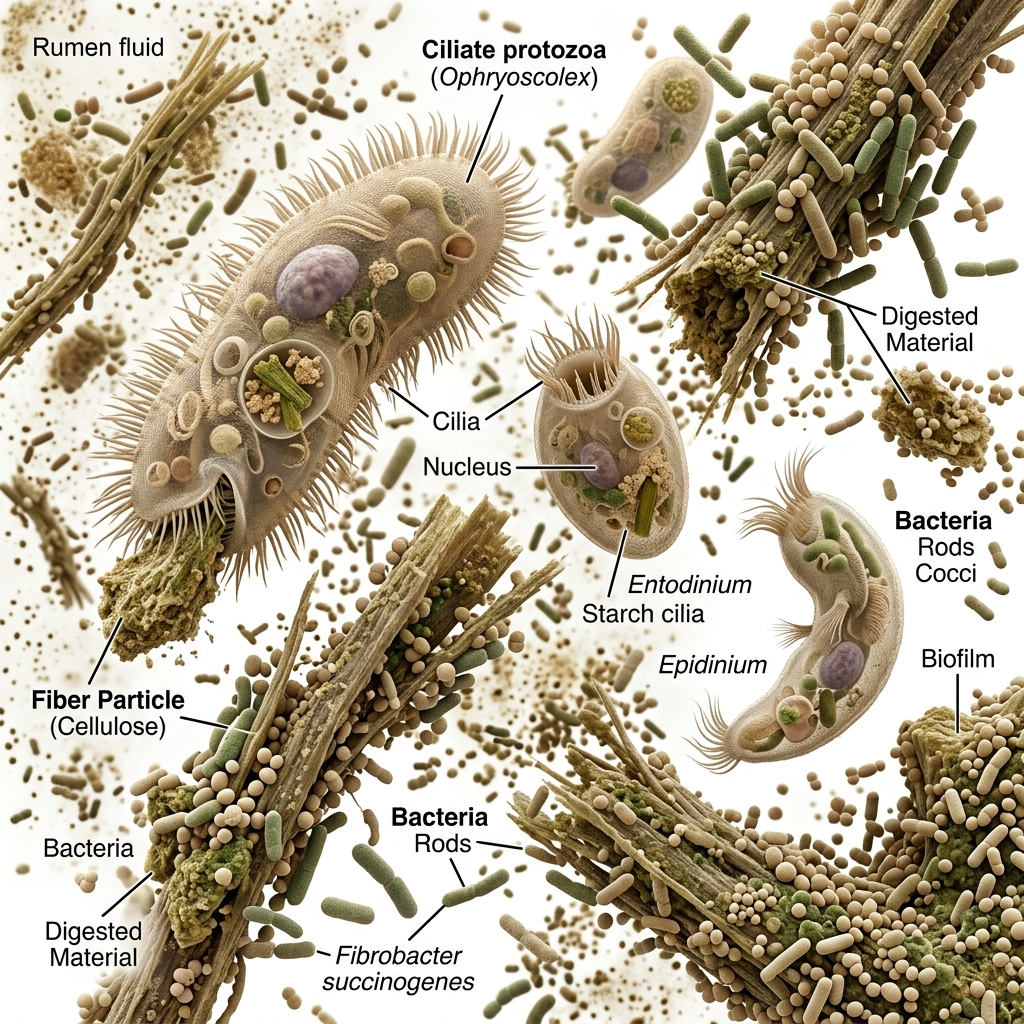
\includegraphics[width=0.85\textwidth]{assets/ch07_rumen_microbes.png}
    \caption{การจำลอง 3D ของระบบนิเวศในรูเมน (Rumen ecosystem) แสดงปฏิสัมพันธ์ระหว่างแบคทีเรียย่อยเยื่อใยพืช โปรโตซัวกลุ่มมีซิเลีย (Ciliates) เส้นใยเชื้อรากระเพาะหมัก (\organism{Neocallimastix}) และกลุ่มอาร์เคียสร้างก๊าซมีเทน (Methanogenic Archaea) ที่เกาะติดและย่อยสลายผนังเซลล์พืชในสภาวะแอนแอโรบิกอย่างสมบูรณ์}
    \label{fig:ch07_rumen_microbes}
\end{figure}

\section*{วัตถุประสงค์การเรียนรู้ประจำบท}
เมื่อศึกษาบทเรียนนี้จบแล้ว นักศึกษาสามารถ:
\begin{enumerate}
    \item อธิบายสรีรวิทยาสภาพแวดล้อมและโครงสร้างความหลากหลายของจุลินทรีย์ในกระเพาะรูเมน (แบคทีเรีย โปรโตซัว รา และอาร์เคีย)
    \item เขียนสมการสโตอิชิโอเมตรีการหมักคาร์โบไฮเดรตในรูเมนเป็นกรดไขมันระเหยง่าย (Acetate, Propionate, Butyrate) และการสร้างก๊าซมีเทน
    \item วิเคราะห์แนวทางการลดการปล่อยก๊าซมีเทนจากสัตว์เคี้ยวเอื้องด้วยสารยับยั้งจำเพาะและโภชนศาสตร์จุลินทรีย์
    \item อธิบายกลไกการเปลี่ยนรูปของเสียไนโตรเจน (TAN $\rightarrow NO_2^- \rightarrow NO_3^-$) และคำนวณการปรับสมดุล C:N Ratio ในระบบไบโอฟล็อก (Biofloc)
    \item วิเคราะห์พยาธิกำเนิดของสารพิษไบนารีท็อกซิน PirA/PirB จากเชื้อ \organism{Vibrio parahaemolyticus} (AHPND) ในกุ้ง และกลไกของโพรไบโอติกในการควบคุมโรค
\end{enumerate}

\section{ระบบนิเวศสรีรวิทยาและสังคมจุลินทรีย์ในกระเพาะรูเมน}

กระเพาะรูเมน (Rumen) ของสัตว์เคี้ยวเอื้อง (โค กระบือ แพะ แกะ) เป็นเครื่องปฏิกรณ์ชีวภาพแบบหมักต่อเนื่องไร้ออกซิเจนขนาดใหญ่ โดยในโคนมโตเต็มวัยมีปริมาตรจุสารหมักได้ถึง $100 - 250\text{ ลิตร}$ สภาพแวดล้อมภายในรูเมนถูกควบคุมอย่างจำเพาะสูง:
\begin{itemize}
    \item \textbf{อุณหภูมิคงที่:} $38.5 - 40.0^\circ\text{C}$
    \item \textbf{ความเป็นกรด-ด่าง (pH):} $5.8 - 6.8$ (ควบคุมด้วยน้ำลายที่มีสารบัฟเฟอร์ไบคาร์บอเนตและฟอสเฟตสูงถึง 150 ลิตรต่อวัน)
    \item \textbf{ศักย์ออกซิเดชัน-รีดักชัน (Redox Potential: $E_h$):} ต่ำกว่า $-350\text{ mV}$ (สภาวะแอนแอโรบิกเข้มงวด)
\end{itemize}

\subsection{องค์ประกอบของสังคมจุลินทรีย์ในรูเมน}
\begin{enumerate}
    \item \textbf{แบคทีเรียในรูเมน (Rumen Bacteria, $10^{10} - 10^{11}\text{ เซลล์/mL}$):}
    \begin{itemize}
        \item \textit{กลุ่มย่อยเซลลูโลสและเฮมิเซลลูโลส (Fibrolytic):} \organism{Fibrobacter succinogenes}\index{Fibrobacter succinogenes@\textit{Fibrobacter succinogenes}}, \organism{Ruminococcus albus}\index{Ruminococcus albus@\textit{Ruminococcus albus}}, และ \organism{Ruminococcus flavefaciens} สร้างเอนไซม์ Cellulase และ Xylanase ย่อยสลายโครงสร้างผนังเซลล์พืช
        \item \textit{กลุ่มย่อยแป้งและน้ำตาล (Amylolytic):} \organism{Streptococcus bovis}\index{Streptococcus bovis@\textit{Streptococcus bovis}}, \organism{Ruminobacter amylophilus}, และ \organism{Succinimonas amylolytica}
        \item \textit{กลุ่มใช้น้ำตาลและกรดแลกติก (Acid-utilizing):} \organism{Megasphaera elsdenii}\index{Megasphaera elsdenii@\textit{Megasphaera elsdenii}} และ \organism{Selenomonas ruminantium} ช่วยเปลี่ยนกรดแลกติกเป็นกรดโพรพิโอนิก ป้องกันภาวะกรดเกินในรูเมน (Acidosis)
    \end{itemize}
    \item \textbf{โปรโตซัวในรูเมน (Rumen Protozoa, $10^5 - 10^6\text{ เซลล์/mL}$):} ส่วนใหญ่เป็นซิลิเอต (Ciliates) เช่น \organism{Entodinium}, \organism{Epidinium}, และ \organism{Polyplastron} ทำหน้าที่กลืนกินเม็ดแป้งอย่างรวดเร็วเพื่อชะลออัตราการหมัก และล่ากินแบคทีเรียเพื่อหมุนเวียนโปรตีน
    \item \textbf{เชื้อราในรูเมน (Anaerobic Gut Fungi, $10^3 - 10^5\text{ ซูโอสปอร์/mL}$):} เช่น สกุล \organism{Neocallimastix}\index{Neocallimastix@\textit{Neocallimastix}}, \organism{Piromyces}, และ \organism{Orpinomyces} เส้นใยไรซอยด์ (Rhizoids) สามารถแทงทะลุเปลือกชั้นลิกนินที่แข็งกระด้างของพืช เปิดทางให้แบคทีเรียแทรกเข้าไปย่อยเนื้อเยื่อภายใน
    \item \textbf{อาร์เคียสร้างมีเทน (Methanogenic Archaea, $10^8 - 10^9\text{ เซลล์/mL}$):} เช่น \organism{Methanobrevibacter ruminantium}\index{Methanobrevibacter ruminantium@\textit{Methanobrevibacter ruminantium}} และ \organism{Methanosphaera stadtmanae} ใช้อิเล็กตรอนและไฮโดรเจนอิสระ ($H_2$) รีดิวซ์คาร์บอนไดออกไซด์เป็นก๊าซมีเทน
\end{enumerate}

\section{สโตอิชิโอเมตรีของการหมักกรดไขมันระเหยง่ายและการสร้างมีเทน}

การย่อยสลายพอลิแซ็กคาไรด์ในรูเมนผ่านกระบวนการไกลโคไลซิสจะได้โมเลกุลน้ำตาลเฮกโซส (Hexose: กลูโคส) จากนั้นถูกหมักผ่านวิถีชีวเคมีต่างๆ เกิดเป็นกรดไขมันระเหยง่าย (Volatile Fatty Acids: VFAs)\index{กรดไขมันระเหยง่าย (Volatile Fatty Acids: VFAs)} 3 ชนิดหลัก:

\subsection{1. ปฏิกิริยาสังเคราะห์กรดอะซิติก (Acetate Pathway)}
\begin{equation}
C_6H_{12}O_6 + 2 H_2O \longrightarrow 2 CH_3COOH + 2 CO_2 + 4 H_2
\end{equation}
ปฏิกิริยานี้ปลดปล่อยก๊าซไฮโดรเจนอิสระออกมามาก ($4\text{ โมล } H_2\text{ ต่อโมลกลูโคส}$) สัตว์นำอะซิเตตไปใช้สังเคราะห์ไขมันในเนื้อเยื่อและไขมันในน้ำนม (Milk fat)\index{กรดอะซิติก (Acetate)}

\subsection{2. ปฏิกิริยาสังเคราะห์กรดบิวไทริก (Butyrate Pathway)}
\begin{equation}
C_6H_{12}O_6 \longrightarrow CH_3CH_2CH_2COOH + 2 CO_2 + 2 H_2
\end{equation}
ปลดปล่อยก๊าซไฮโดรเจน $2\text{ โมล } H_2$ สัตว์นำบิวไทเรตไปใช้เป็นพลังงานของเซลล์บุผนังกระเพาะรูเมน (Rumen papillae)\index{กรดบิวไทริก (Butyrate)}

\subsection{3. ปฏิกิริยาสังเคราะห์กรดโพรพิโอนิก (Propionate Pathway)}
ดำเนินผ่านวิถีซักซิเนต (Succinate pathway) หรือวิถีอะคริเลต (Acrylate pathway):\index{กรดโพรพิโอนิก (Propionate)}
\begin{equation}
C_6H_{12}O_6 + 2 H_2 \longrightarrow 2 CH_3CH_2COOH + 2 H_2O
\end{equation}
ปฏิกิริยานี้ **บริโภคไฮโดรเจนอิสระ ($2\text{ โมล } H_2$)** เข้าไปในโมเลกุล กรดโพรพิโอเนตจะถูกดูดซึมส่งไปยังตับเพื่อสังเคราะห์เป็นน้ำตาลกลูโคส (Gluconeogenesis) ซึ่งเป็นแหล่งพลังงานหลักของร่างกายและการเจริญเติบโต

\subsection{4. กระบวนการสร้างก๊าซมีเทน (Methanogenesis) และการควบคุม}
ก๊าซไฮโดรเจน ($H_2$) ที่เกิดขึ้นจากวิถีอะซิเตตและบิวไทเรต หากสะสมมากเกินไปจะยับยั้งเอนไซม์ดีไฮโดรจีเนสและหยุดการทำงานของจุลินทรีย์ทั้งระบบ อาร์เคียสร้างมีเทนจึงทำหน้าที่เป็นถังรับไฮโดรเจน (Hydrogen sink):
\begin{equation}
CO_2 + 4 H_2 \longrightarrow CH_4 + 2 H_2O \quad (\Delta G^\circ = -131\text{ kJ/mol})
\end{equation}
อย่างไรก็ดี ก๊าซมีเทนที่สัตว์เรอออกมาคิดเป็นการสูญเสียพลังงานของอาหารสัตว์ถึงร้อยละ 6--12 และเป็นก๊าซเรือนกระจกที่มีศักยภาพโลกร้อนสูงกว่า $CO_2$ ถึง 28 เท่า ในปัจจุบันมีการใช้สารยับยั้งทางชีวเคมี เช่น สารสกัดสาหร่ายสีแดง (\organism{Asparagopsis taxiformis}) ซึ่งมีสารโบรโมฟอร์ม (Bromoform) หรือสาร 3-Nitrooxypropanol (3-NOP) ยับยั้งเอนไซม์ Methyl-coenzyme M reductase (MCR) ช่วยลดการปล่อยมีเทนได้มากกว่า $30 - 80\%$

\section{จุลชีววิทยาทางเพาะเลี้ยงสัตว์น้ำและวงจรไนโตรเจน}

ในการเพาะเลี้ยงกุ้งและปลาหนาแน่นสูง อาหารเม็ดโปรตีนสูงที่สัตว์กินและขับถ่ายออกมารวมทั้งอาหารที่เหลือตกค้าง จะสลายตัวกลายเป็น \textbf{ไนโตรเจนแอมโมเนียรวม (Total Ammonia Nitrogen: TAN)\index{แอมโมเนียรวม (TAN: Total Ammonia Nitrogen)}}:

\begin{equation}
\text{TAN} = [NH_3] + [NH_4^+]
\end{equation}

สัดส่วนของแอมโมเนียอิสระไร้ประจุ ($NH_3$) ซึ่งมีความเป็นพิษสูงมากต่อเหงือกและระบบประสาทของสัตว์น้ำ จะแปรผันตามค่า pH และอุณหภูมิของน้ำ:

\begin{equation}
\% NH_3 = \frac{100}{1 + 10^{(pK_a - \text{pH})}}
\end{equation}

เมื่อ $pK_a \approx 9.24$ ที่อุณหภูมิ $28^\circ\text{C}$ หากน้ำในบ่อมีค่า $\text{pH } 8.5$ สัดส่วนของ $NH_3$ จะสูงถึงประมาณ $15\%$ ของ TAN ทั้งหมด ซึ่งเป็นอันตรายถึงชีวิตต่อสัตว์น้ำหาก TAN เกิน $1 - 2\text{ mg/L}$

\subsection{1. กระบวนการไนตริฟิเคชันแบบออโตโทรฟิก (Autotrophic Nitrification)}
ในระบบกรองชีวภาพ (Biofilter) แบคทีเรียไนตริฟายเออร์จะทำปฏิกิริยาออกซิเดชันสองขั้นตอน:
\begin{itemize}
    \item แอมโมเนียออกซิไดซิงแบคทีเรีย (AOB: เช่น \organism{Nitrosomonas}):
    $$2 NH_4^+ + 3 O_2 \longrightarrow 2 NO_2^- + 4 H^+ + 2 H_2O$$
    \item ไนไตรต์ออกซิไดซิงแบคทีเรีย (NOB: เช่น \organism{Nitrobacter}, \organism{Nitrospira}):
    $$2 NO_2^- + O_2 \longrightarrow 2 NO_3^-$$
\end{itemize}
กระบวนการนี้ต้องการออกซิเจนสูง ($4.57\text{ g } O_2$ ต่อน้ำหนัก $1\text{ g } NH_4^+$-N) และทำลายความเป็นด่าง (Alkalinity) ในน้ำ โดยกินด่างไปถึง $7.14\text{ g } CaCO_3$ ต่อน้ำหนัก $1\text{ g } NH_4^+$-N ผู้เลี้ยงจึงต้องเติมปูนขาวหรือโซเดียมไบคาร์บอเนตอย่างสม่ำเสมอ

\subsection{2. เทคโนโลยีไบโอฟล็อก (Biofloc Technology: BFT)}
แทนที่จะพึ่งพาแบคทีเรียออโตโทรฟที่เติบโตช้า ระบบ Biofloc\index{เทคโนโลยีไบโอฟล็อก (Biofloc Technology: BFT)} อาศัยการเติมนิ่งคาร์บอน (เช่น กากน้ำตาล รำข้าว แป้งมันสำปะหลัง) เพื่อปรับอัตราส่วนคาร์บอนต่อไนโตรเจน (\textbf{C:N Ratio $\ge 15:1$}\index{อัตราส่วน C:N (Carbon-to-Nitrogen Ratio)}):
\begin{itemize}
    \item แบคทีเรียกลุ่ม \textbf{Heterotrophic Bacteria\index{แบคทีเรียเฮเทอโรโทรฟิก (Heterotrophic Bacteria)}} จะใช้น้ำตาลเป็นแหล่งพลังงานและดูดซับแอมโมเนียมไอออน ($NH_4^+$) เข้าไปสังเคราะห์เป็นโปรตีนเซลล์จุลินทรีย์ (Single-Cell Protein) อย่างรวดเร็ว (เร็วกว่าไนตริฟิเคชัน 10 เท่า)
    \item แบคทีเรียจะสร้างสารพอลิเมอร์นอกเซลล์ (EPS) จับตัวกับแพลงก์ตอนพืชและโปรโตซัว รวมกันเป็นตะกอนแขวนลอยเรียกว่า \textbf{ก้อนฟล็อก (Biofloc)}
    \item กุ้งและปลาสามารถตอดกินก้อนฟล็อกเป็นอาหารโปรตีนธรรมชาติ (มีโปรตีน $25 - 35\%$) ช่วยลดอัตราการใช้อาหารเม็ด (FCR) และลดการเปลี่ยนถ่ายน้ำสู่สิ่งแวดล้อมภายนอกได้เกือบ $100\%$
\end{itemize}

\begin{figure}[ht]
\centering
\begin{tikzpicture}[
    scale=0.88, every node/.style={scale=0.88},
    box/.style={draw=navyprimary, fill=white, rounded corners=5pt, text width=3.4cm, align=center, line width=1pt},
    patha/.style={draw=blue!80!black, fill=blue!8, rounded corners=5pt, text width=3.3cm, align=center, line width=1pt},
    pathb/.style={draw=forestgreen, fill=forestgreen!10, rounded corners=5pt, text width=3.3cm, align=center, line width=1pt},
    arrow/.style={->, >=Stealth, line width=1.3pt}
]
    % Central source
    \node [box, fill=amber!15] (source) at (6, 4.5) {
        \textbf{ไนโตรเจนแอมโมเนียรวม}\\\textbf{(TAN: $NH_3 / NH_4^+$)}\\[2pt]
        {\scriptsize จากอาหารตกค้างและการขับถ่าย}
    };

    % Pathway A: Autotrophic Nitrification
    \node [patha] (nit1) at (2.2, 2.5) {
        \textbf{1. ไนไตรต์ ($NO_2^-$)}\\[2pt]
        {\scriptsize ออกซิไดซ์โดย AOB\\(\organism{Nitrosomonas})}
    };
    \node [patha] (nit2) at (2.2, 0.5) {
        \textbf{2. ไนเตรต ($NO_3^-$)}\\[2pt]
        {\scriptsize ออกซิไดซ์โดย NOB\\(\organism{Nitrobacter})}
    };
    \node [patha, fill=blue!15] (nita_sum) at (2.2, -1.5) {
        \textbf{ระบบไนตริฟิเคชันดั้งเดิม}\\[2pt]
        {\scriptsize $\bullet$ สิ้นเปลือง $O_2$ สูง\\$\bullet$ กินด่าง $7.14\text{ g } CaCO_3/\text{g N}$\\$\bullet$ ต้องถ่ายน้ำระบาย $NO_3^-$}
    };

    % Pathway B: Heterotrophic Biofloc
    \node [pathb] (bio1) at (9.8, 2.5) {
        \textbf{1. เติมคาร์บอน (C:N $\ge$ 15)}\\[2pt]
        {\scriptsize กากน้ำตาล / รำข้าว / แป้ง}
    };
    \node [pathb] (bio2) at (9.8, 0.5) {
        \textbf{2. การดูดซึมเร็ว}\\[2pt]
        {\scriptsize แบคทีเรีย Heterotrophs\\สังเคราะห์โปรตีนเซลล์}
    };
    \node [pathb, fill=forestgreen!20] (biob_sum) at (9.8, -1.5) {
        \textbf{ก้อนฟล็อกโปรตีน (Biofloc)}\\[2pt]
        {\scriptsize $\bullet$ กุ้ง/ปลาตอดกิน (ลด FCR)\\$\bullet$ ไม่ต้องเปลี่ยนถ่ายน้ำ ($0\%$)\\$\bullet$ กำจัด TAN เร็วกว่า 10 เท่า}
    };

    % Arrows Pathway A
    \draw [arrow, blue!80!black] (source) -| (nit1) node[midway, above left, font=\scriptsize] {Autotrophic};
    \draw [arrow, blue!80!black] (nit1) -- (nit2) node[midway, right, font=\scriptsize] {$+ O_2$};
    \draw [arrow, blue!80!black] (nit2) -- (nita_sum);

    % Arrows Pathway B
    \draw [arrow, forestgreen] (source) -| (bio1) node[midway, above right, font=\scriptsize] {Heterotrophic};
    \draw [arrow, forestgreen] (bio1) -- (bio2) node[midway, right, font=\scriptsize] {$+ NH_4^+$};
    \draw [arrow, forestgreen] (bio2) -- (biob_sum);

\end{tikzpicture}
\caption{การเปรียบเทียบพลวัตการกำจัดไนโตรเจนแอมโมเนียในบ่อเพาะเลี้ยงสัตว์น้ำ: ระบบกรองชีวภาพแบบไนตริฟิเคชันดั้งเดิม (Autotrophic Nitrification) กับเทคโนโลยีไบโอฟล็อก (Heterotrophic Biofloc Technology: BFT)}
\label{fig:aquaculture_nitrogen_pathways}
\end{figure}

\section{โรคตายด่วนในกุ้ง (AHPND/EMS) และการใช้โพรไบโอติกควบคุม}

\subsection{1. ชีวโมเลกุลสารพิษ PirA/PirB ของเชื้อ Vibrio parahaemolyticus}
โรคตับวายเฉียบพลันในกุ้ง (Acute Hepatopancreatic Necrosis Disease: AHPND หรือ EMS) เกิดจากแบคทีเรีย \organism{Vibrio parahaemolyticus} สายพันธุ์ก่อโรคที่มีพลาสมิด pVA1 ขนาด $69 - 73\text{ kb}$ ซึ่งมียีนสร้างสารพิษไบนารีท็อกซิน **PirA$^{vp}$ ($13\text{ kDa}$)** และ **PirB$^{vp}$ ($50\text{ kDa}$)**:
\begin{itemize}
    \item สารพิษ PirA และ PirB รวมตัวกันเป็นสารเชิงซ้อน (Heterodimer complex) ซึ่งมีโครงสร้างคล้ายสารพิษฆ่าแมลง Pir toxin ของแบคทีเรีย \organism{Photorhabdus}
    \item โปรตีน PirB เข้าจับกับตัวรับบนเยื่อหุ้มเซลล์ของท่อน้ำดีและตับอ่อนของกุ้ง (Hepatopancreas) จากนั้นแทงสร้างรูรั่ว นำพา PirA เข้าสู่เซลล์
    \item เซลล์ท่อตับอ่อนหลุดลอก (Massive Sloughing) ส่งผลให้เนื้อเยื่อตับอ่อนฝ่อลีบ ซีดขาว และกุ้งตายเกลื่อนบ่อภายใน $10 - 35\text{ วัน}$ หลังปล่อยลูกกุ้ง
\end{itemize}

\subsection{2. กลไกการออกฤทธิ์ของโพรไบโอติกในระบบทางเดินอาหารสัตว์น้ำ}
การเสริมแบคทีเรียโพรไบโอติก เช่น \organism{Bacillus subtilis}, \organism{Bacillus licheniformis}, และ \organism{Lactobacillus plantarum} ในอาหารกุ้งช่วยต้านทานเชื้อ \organism{Vibrio} ผ่าน 3 กลไกหลัก:
\begin{enumerate}
    \item \textbf{Quorum Quenching:} แบคทีเรีย \organism{Bacillus} สังเคราะห์เอนไซม์ **AHL Lactonase** สลายโมเลกุลส่งสัญญาณสื่อสารระหว่างเซลล์ (Acyl-Homoserine Lactone: AHL) ของเชื้อ \organism{Vibrio} ทำให้เชื้อไม่สามารถรวมกลุ่มสั่งการหลั่งสารพิษ PirA/PirB ได้
    \item \textbf{Competitive Exclusion:} เข้ายึดเกาะตัวรับบนเยื่อบุลำไส้กุ้งและผลิตสารแบคเทอริโอซิน (Bacteriocins) ยับยั้งการเจริญเติบโตของเชื้อก่อโรค
    \item \textbf{การกระตุ้นภูมิคุ้มกันกุ้ง (ProPO System):} ผนังเซลล์ของโปรไบโอติก ($\beta$-glucans และ Lipopolysaccharides) กระตุ้นการทำงานของเอนไซม์ Prophenoloxidase (ProPO) ในเม็ดเลือดกุ้ง ช่วยสังเคราะห์เมลานินเข้าห่อหุ้มและทำลายเชื้อก่อโรค
\end{enumerate}

\begin{worked}[ตัวอย่างที่ 7.1 การคำนวณสัดส่วน VFAs และการปลดปล่อยพลังงานจากการหมักในรูเมน]
ในโคเนื้อที่กินหญ้าแห้งเป็นอาหารหลัก จุลินทรีย์ในรูเมนผลิตกรดไขมันระเหยง่ายด้วยอัตราส่วนโมลาร์ดังนี้:
$$\text{Acetate } (A) : \text{Propionate } (P) : \text{Butyrate } (B) = 65 : 20 : 15$$
หากการหมักเริ่มต้นจากโมเลกุลกลูโคส 100 โมล จงคำนวณปริมาณไฮโดรเจนอิสระ ($H_2$) สุทธิที่เกิดขึ้น และคำนวณปริมาณก๊าซมีเทน ($CH_4$) ที่ถูกสร้างขึ้นตามทฤษฎี

\textbf{วิธีทำ:}
1. จากสมการสโตอิชิโอเมตรี:
\begin{itemize}
    \item 1 โมล Glucose $\rightarrow$ 2 โมล Acetate $+ 4$ โมล $H_2$ $\implies$ ผลิต $H_2 = 2.0\text{ โมลต่อโมล Acetate}$
    \item 1 โมล Glucose $\rightarrow$ 1 โมล Butyrate $+ 2$ โมล $H_2$ $\implies$ ผลิต $H_2 = 2.0\text{ โมลต่อโมล Butyrate}$
    \item 1 โมล Glucose $+ 2$ โมล $H_2 \rightarrow$ 2 โมล Propionate $\implies$ บริโภค $H_2 = 1.0\text{ โมลต่อโมล Propionate}$
\end{itemize}

2. คำนวณสมดุล $H_2$ จากสัดส่วนโมลาร์ $65A : 20P : 15B$:
$$H_{2\text{ สร้างขึ้น}} = (65 \times 2.0) + (15 \times 2.0) = 130 + 30 = 160\text{ โมล } H_2$$
$$H_{2\text{ บริโภค}} = 20 \times 1.0 = 20\text{ โมล } H_2$$
$$H_{2\text{ สุทธิ}} = 160 - 20 = 140\text{ โมล } H_2$$

3. คำนวณปริมาณมีเทน ($CH_4$) จากสมการ $CO_2 + 4 H_2 \rightarrow CH_4 + 2 H_2O$:
$$CH_4 = \frac{H_{2\text{ สุทธิ}}}{4} = \frac{140}{4} = 35.0\text{ โมล } CH_4$$

\textbf{บทวิเคราะห์ผลลัพธ์:} ในอาหารเยื่อใยสูง เกิดมีเทนถึง 35 โมลต่อ 100 โมลของผลผลิต VFAs หากเราเสริมอาหารข้นเพื่อปรับสัดส่วน Propionate ให้เพิ่มขึ้นเป็น 35\% ไฮโดรเจนสุทธิจะลดลงเหลือ $100\text{ โมล}$ ส่งผลให้การปล่อยมีเทนลดลงเหลือเพียง $25\text{ โมล}$ (ลดลงถึง 28.6\%) ซึ่งยืนยันว่าการจัดการโภชนศาสตร์อาหารสัตว์มีผลโดยตรงต่อการลดภาวะโลกร้อน
\end{worked}

\begin{worked}[ตัวอย่างที่ 7.2 การคำนวณปริมาณกากน้ำตาลเพื่อปรับ C:N Ratio ในบ่อกุ้งระบบ Biofloc]
บ่อเพาะเลี้ยงกุ้งขาวแวนนาไมความหนาแน่นสูงมีปริมาตรน้ำ $200\text{ m}^3$ จากการตรวจวัดคุณภาพน้ำ พบค่าแอมโมเนียไนโตรเจนรวม $\text{TAN} = 3.5\text{ mg/L}$ ($= 3.5\text{ g/m}^3$) 

เกษตรกรต้องการเติม **กากน้ำตาล (Molasses)** ซึ่งมีคาร์บอนอินทรีย์ร้อยละ 40 โดยน้ำหนัก เพื่อปรับอัตราส่วน C:N เป็น $16:1$ เพื่อให้แบคทีเรียกลุ่มเฮเทอโรโทรฟตรึงแอมโมเนียทั้งหมดให้เป็นมวลชีวภาพ จงคำนวณหาน้ำหนักกากน้ำตาลที่ต้องใส่ลงในบ่อ

\textbf{วิธีทำ:}
1. คำนวณปริมาณไนโตรเจน TAN ทั้งหมดในบ่อน้ำ:
$$N_{\text{total}} = \text{TAN} \times V_{\text{pond}} = 3.5\text{ g/m}^3 \times 200\text{ m}^3 = 700\text{ g } N = 0.70\text{ kg } N$$

2. คำนวณปริมาณคาร์บอนอินทรีย์ที่ต้องการสำหรับ $\text{C:N} = 16:1$:
$$C_{\text{required}} = N_{\text{total}} \times 16 = 0.70\text{ kg } \times 16 = 11.20\text{ kg } C$$

3. คำนวณน้ำหนักกากน้ำตาลที่ต้องใช้ (กากน้ำตาลมี $C = 40\%$ หรือ 0.40):
$$W_{\text{molasses}} = \frac{C_{\text{required}}}{0.40} = \frac{11.20\text{ kg}}{0.40} = 28.0\text{ kg}$$

\textbf{บทวิเคราะห์ผลลัพธ์:} การเติมกากน้ำตาลปริมาณ $28.0\text{ kg}$ พร้อมทั้งเปิดเครื่องตีน้ำให้ออกซิเจนละลายน้ำสูงกว่า $5\text{ mg/L}$ จะกระตุ้นให้แบคทีเรียเปลี่ยนแอมโมเนียที่มีพิษเป็นก้อนตะกอนโปรตีนไบโอฟล็อกจนค่า TAN ลดลงต่ำกว่า $0.5\text{ mg/L}$ ภายในเวลา $24 - 48\text{ ชั่วโมง}$
\end{worked}

% [RESEARCH-UPDATE-2026-10]
\section{ความก้าวหน้างานวิจัยล่าสุดด้านจุลินทรีย์ในปศุสัตว์และสัตว์น้ำ}

รายงานการวิจัยระดับนานาชาติในปี ค.ศ. 2024–2026 โดย Wang และคณะ \cite{pmid41153915} ได้แสดงหลักฐานชัดเจนว่าการเสริมสารโพสต์ไบโอติก (Postbiotics: สารสกัดไร้เซลล์ที่ประกอบด้วย SCFA และ bacteriocins) ในอาหารสัตว์ ช่วยลดการอักเสบของลำไส้ในสุกรและสัตว์ปีกได้อย่างมีนัยสำคัญโดยไม่ต้องกังวลเรื่องการตายของเซลล์จุลินทรีย์ระหว่างกระบวนการอัดเม็ดอาหารความร้อนสูง

ในด้านการหมักรูเมน งานวิจัยทางเมตาโปรตีโอมิกส์ของ Cuno และคณะ \cite{pmid37169869} เผยให้เห็นว่าโปรโตซัวกลุ่ม Holotrich ciliates มีบทบาทหลักในการกักเก็บคาร์โบไฮเดรตในรูปพอลิเมอร์ และปล่อยสารอาหารกลับออกมาอย่างช้าๆ ช่วยรักษาเสถียรภาพค่า pH และป้องกันการเกิดกรดเฉียบพลันในกระเพาะหมักของโคนมพันธุ์ผลผลิตสูง

\begin{insight}[ประเด็นวิเคราะห์เชิงวิชาการ]
เกษตรกรผู้เลี้ยงกุ้งบางท่านประสบปัญหาว่า เมื่อเติมกากน้ำตาลเพื่อสร้างระบบ Biofloc มากเกินไป ค่าออกซิเจนละลายน้ำ (DO) ในเวลากลางคืนกลับลดลงอย่างรวดเร็วจนกุ้งลอยหัว จงอธิบายปรากฏการณ์นี้ในเชิงจุลชีววิทยาและพลวัตการใช้ออกซิเจนของแบคทีเรีย
\end{insight}

\section*{สรุปประจำบท}

จุลชีววิทยาในระบบปศุสัตว์และเพาะเลี้ยงสัตว์น้ำเป็นหัวใจของการบริหารจัดการห่วงโซ่โปรตีนของโลก สังคมจุลินทรีย์ในกระเพาะรูเมนของสัตว์เคี้ยวเอื้องทำหน้าที่ย่อยสลายเซลลูโลสผ่านปฏิกิริยาสโตอิชิโอเมตรีที่ให้ผลผลิตเป็นกรดไขมันระเหยง่าย (Acetate, Propionate, Butyrate) ซึ่งอัตราส่วนของ VFAs มีผลโดยตรงต่อการปล่อยก๊าซมีเทนของอาร์เคีย ในภาคการเพาะเลี้ยงสัตว์น้ำ การจัดการวงจรไนโตรเจนด้วยระบบไนตริฟิเคชันและระบบไบโอฟล็อก (C:N $\ge 15:1$) ช่วยเปลี่ยนแอมโมเนียมีพิษให้กลายเป็นตะกอนโปรตีนธรรมชาติ ขณะเดียวกัน การใช้แบคทีเรียโพรไบโอติกที่หลั่งเอนไซม์ทำลายระบบสื่อสาร Quorum Sensing และสร้างสารแบคเทอริโอซิน ถือเป็นเกราะป้องกันทางชีวภาพที่ทรงประสิทธิภาพในการระงับสารพิษ PirA/PirB ของเชื้อ \organism{Vibrio parahaemolyticus} ในกุ้งได้อย่างยั่งยืน

\subsection*{คำถามท้ายบทและการวิเคราะห์}

\noindent \textbf{ระดับที่ 1: ความรู้และความเข้าใจเชิงทฤษฎี (Knowledge \& Comprehension)}
\begin{enumerate}
    \item สรุปหน้าที่และปฏิสัมพันธ์ระหว่างสิ่งมีชีวิต 4 กลุ่มหลักในรูเมน (แบคทีเรีย โปรโตซัว เชื้อรากระเพาะหมัก และอาร์เคีย)
    \item เขียนสมการเคมีเปรียบเทียบระหว่างวิถีการสังเคราะห์ Acetate และ Propionate ในกระเพาะรูเมน พร้อมอธิบายว่าวิถีใดส่งเสริมการสร้างก๊าซมีเทนมากกว่า เพราะเหตุใด?
    \item อธิบายกลไกของสาร 3-NOP (3-Nitrooxypropanol) ในการยับยั้งกระบวนการสังเคราะห์ก๊าซมีเทนในกระเพาะรูเมน
    \item ความเป็นกรด-ด่าง (pH) และอุณหภูมิของน้ำส่งผลต่อสมดุลระหว่าง $NH_3$ และ $NH_4^+$ อย่างไร? และฟอร์มใดเป็นอันตรายต่อสัตว์น้ำมากกว่า?
\end{enumerate}

\noindent \textbf{ระดับที่ 2: การวิเคราะห์และการคำนวณเชิงปริมาณ (Quantitative Analysis \& Calculation)}
\begin{enumerate}[resume]
    \item ในระบบการกรองชีวภาพแบบดั้งเดิม เหตุใดการเกิดไนตริฟิเคชันจึงส่งผลให้ค่าความเป็นด่าง (Alkalinity) ของน้ำลดลงอย่างต่อเนื่อง?
    \item ในบ่อเลี้ยงปลานิลปริมาตร $500\text{ m}^3$ มีปริมาณแอมโมเนีย $\text{TAN} = 2.0\text{ mg/L}$ ต้องการปรับสัดส่วน C:N เป็น $15:1$ โดยใช้รำข้าวที่มีคาร์บอนร้อยละ 50 จงคำนวณหาน้ำหนักรำข้าวที่ต้องเติม
    \item สารพิษ PirA และ PirB ของเชื้อ \organism{Vibrio parahaemolyticus} มีบทบาทและกลไกการทำลายเนื้อเยื่อตับอ่อนของกุ้งอย่างไร?
\end{enumerate}

\noindent \textbf{ระดับที่ 3: การสังเคราะห์และการแก้ปัญหาในแปลงจริง (Application \& Real-World Synthesis)}
\begin{enumerate}[resume]
    \item อธิบายหลักการของเทคโนโลยีไบโอฟล็อก (Biofloc Technology) ในการกำจัดแอมโมเนีย และข้อดีเมื่อเปรียบเทียบกับระบบบำบัดแบบไนตริฟิเคชันในบ่อกุ้ง
    \item แบคทีเรียกลุ่ม \organism{Bacillus} ใช้กลไก Quorum Quenching อย่างไรในการระงับความรุนแรงของเชื้อแบคทีเรียก่อโรคในสัตว์น้ำ และประยุกต์ใช้ในฟาร์มเพาะเลี้ยงอย่างไร?
    \item จงออกแบบแนวทางการจัดการฟาร์มโคนมเชิงนิเวศ ที่สามารถลดการปล่อยก๊าซเรือนกระจกจากกระเพาะรูเมน ควบคู่ไปกับการรักษาปริมาณผลผลิตน้ำนมและไขมันนมให้ได้มาตรฐาน
\end{enumerate}

\chapter{วิศวกรรมปุ๋ยหมัก การย่อยสลายลิกโนเซลลูโลส และพลังงานชีวภาพ}
\label{ch:waste_bioenergy}

\begin{keyconcept}[แนวคิดสำคัญของบทที่ 8]
ของเสียและผลพลอยได้ทางการเกษตร เช่น ฟางข้าว ชานอ้อย ทะลายปาล์ม และมูลสัตว์ เป็นชีวมวลที่มีสารประกอบลิกโนเซลลูโลส (Lignocellulose)\index{สารประกอบลิกโนเซลลูโลส (Lignocellulose)} เป็นองค์ประกอบหลัก ซึ่งทนทานต่อการย่อยสลายทางชีวภาพ การประยุกต์ใช้เอนไซม์จากจุลินทรีย์ (Cellulases, Xylanases, Laccases)\index{เอนไซม์เซลลูเลส (Cellulase Complex)}\index{เอนไซม์แลคเคส (Laccase)} ร่วมกับการควบคุมสภาวะทางวิศวกรรม สามารถเปลี่ยนของเสียเหล่านี้ให้กลายเป็นปุ๋ยอินทรีย์ปรับปรุงดินและพลังงานทดแทน การทำปุ๋ยหมัก (Composting)\index{การทำปุ๋ยหมัก (Composting)} อาศัยการสืบทอดสังคมจุลินทรีย์ (Microbial Succession)\index{การสืบทอดสังคมจุลินทรีย์ (Microbial Succession)} ในสภาวะมีออกซิเจนที่อุณหภูมิสูงกว่า 55\degree C เพื่อทำลายเชื้อโรคและวัชพืช ขณะที่กระบวนการย่อยสลายไร้ออกซิเจน (Anaerobic Digestion: AD)\index{การย่อยสลายไร้ออกซิเจน (Anaerobic Digestion)} อาศัยการทำงานประสานกันของแบคทีเรียและอาร์เคียสร้างมีเทน 4 ขั้นตอน ซึ่งสามารถทำนายอัตราการผลิตก๊าซชีวภาพได้อย่างแม่นยำด้วยแบบจำลอง Modified Gompertz Model\index{แบบจำลอง Modified Gompertz (Modified Gompertz Model)}
\end{keyconcept}

\begin{figure}[ht]
    \centering
    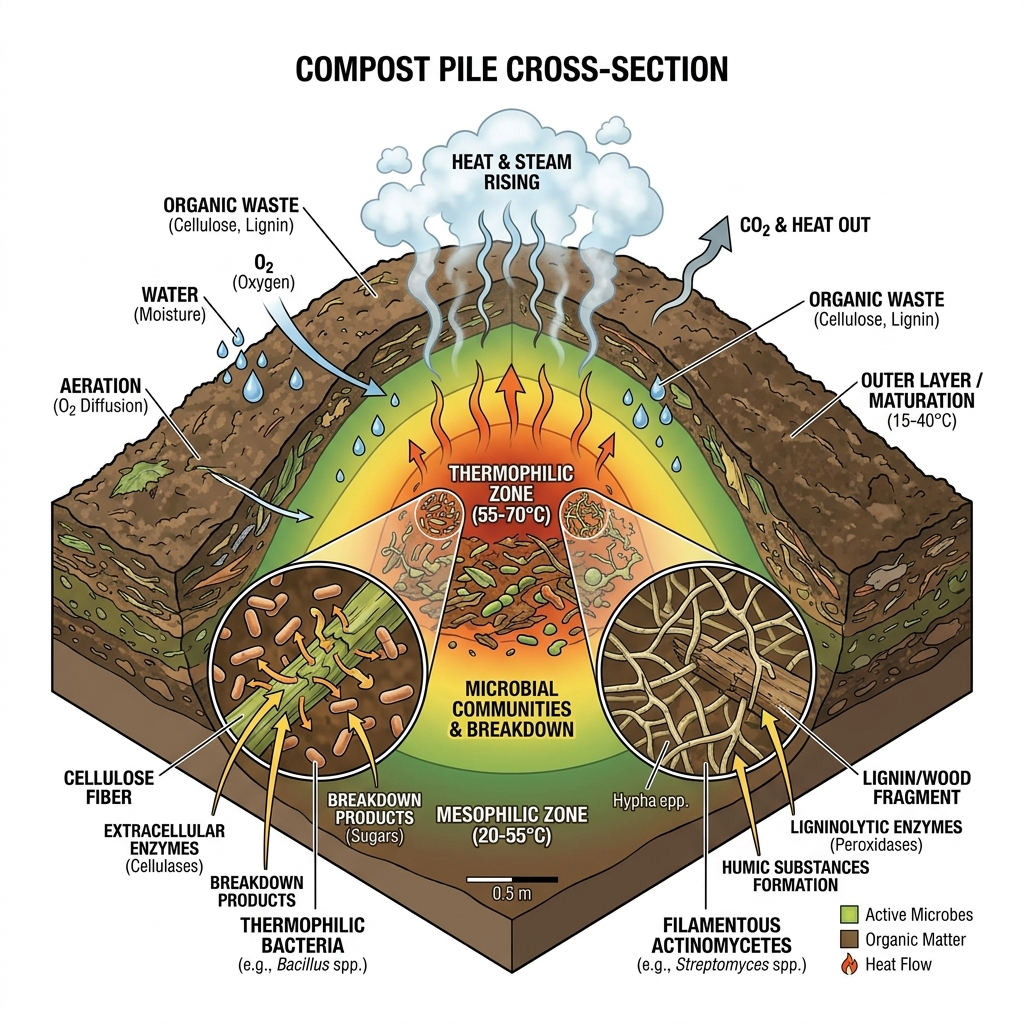
\includegraphics[width=0.85\textwidth]{assets/ch08_composting_microbes.png}
    \caption{การจำลอง 3D แสดงการสืบทอดทางนิเวศวิทยาของจุลินทรีย์ในกองปุ๋ยหมัก (Compost microbial succession) แสดงการเปลี่ยนผ่านจากระยะเริ่มต้นอุณหภูมิปานกลาง (Mesophilic) สู่ระยะอุณหภูมิสูง (Thermophilic phase) ซึ่งแบคทีเรียทนร้อนและแอคติโนมัยซีสย่อยสลายสารอินทรีย์อย่างรวดเร็ว ทำลายเชื้อก่อโรคพืช ก่อนลดอุณหภูมิลงสู่ระยะบ่มตัว (Curing phase)}
    \label{fig:ch08_composting_microbes}
\end{figure}

\section*{วัตถุประสงค์การเรียนรู้ประจำบท}
เมื่อศึกษาบทเรียนนี้จบแล้ว นักศึกษาสามารถ:
\begin{enumerate}
    \item อธิบายโครงสร้างระดับโมเลกุลของลิกโนเซลลูโลส และระบบเอนไซม์ย่อยสลายของจุลินทรีย์ (Cellulase complex และ Lignin-modifying enzymes)
    \item วิเคราะห์พลวัตการสืบทอดของประชากรจุลินทรีย์ทั้ง 4 ระยะในกระบวนการทำปุ๋ยหมักแบบใช้ออกซิเจน
    \item คำนวณระบบสมการดุลมวลสารเพื่อปรับอัตราส่วน C:N และความชื้นของกองปุ๋ยหมักให้ได้เกณฑ์มาตรฐาน
    \item อธิบาย 4 ขั้นตอนเคมีชีวภาพของการย่อยสลายไร้ออกซิเจน (Hydrolysis, Acidogenesis, Acetogenesis, Methanogenesis)
    \item คำนวณและทำนายผลผลิตก๊าซมีเทนสะสมด้วยแบบจำลองจลนศาสตร์ Modified Gompertz Model
\end{enumerate}

\section{ชีวเคมีของการย่อยสลายสารประกอบลิกโนเซลลูโลส}

ชีวมวลพืชประกอบด้วยโครงสร้างพอลิเมอร์ธรรมชาติที่สลับซับซ้อน 3 ชนิดที่ประสานกันอย่างเหนียวแน่น เรียกว่า **ลิกโนเซลลูโลส (Lignocellulose)**:
\begin{enumerate}
    \item \textbf{เซลลูโลส (Cellulose, 40--50\%):} สายพอลิเมอร์เส้นตรงของกลูโคสที่เชื่อมกันด้วยพันธะ $\beta$-1,4-glycosidic ยึดเหนี่ยวกันด้วยพันธะไฮโดรเจนกลายเป็นเส้นใยไมโครไฟบริล (Microfibrils) ที่มีทั้งบริเวณอสัณฐาน (Amorphous) และบริเวณผลึกแน่น (Crystalline region)
    \item \textbf{เฮมิเซลลูโลส (Hemicellulose, 25--35\%):} พอลิแซ็กคาไรด์สายกิ่งที่ประกอบด้วยน้ำตาลเพนโทส (Xylose, Arabinose) และเฮกโซส (Mannose, Galactose, Glucose)
    \item \textbf{ลิกนิน (Lignin, 15--25\%):} พอลิเมอร์อสัณฐานไม่สม่ำเสมอของสารประกอบฟีนอลิก (Phenylpropane units) 3 ชนิด ได้แก่ $p$-coumaryl alcohol, coniferyl alcohol, และ sinapyl alcohol เชื่อมกันด้วยพันธะอีเทอร์ (Ether bonds: $\beta$-O-4) และพันธะคาร์บอน-คาร์บอน (C-C) ที่ทนทานต่อการย่อยสลายทางเคมีมากที่สุด
\end{enumerate}

\subsection{ระบบเอนไซม์ย่อยสลายลิกโนเซลลูโลสของจุลินทรีย์}
\begin{itemize}
    \item \textbf{ระบบเอนไซม์เซลลูเลส (Cellulase Enzyme Complex):} ประกอบด้วยเอนไซม์ 3 ชนิดที่ทำงานเสริมฤทธิ์กัน:
    \begin{enumerate}
        \item \textit{Endo-$\beta$-1,4-glucanase (EC 3.2.1.4):} สุ่มตัดพันธะภายในสายเซลลูโลสบริเวณอสัณฐาน สร้างปลายสายอิสระ
        \item \textit{Exo-$\beta$-1,4-glucanase หรือ Cellobiohydrolase (EC 3.2.1.91):} ตัดน้ำตาลไดแซ็กคาไรด์ **เซลโลไบโอส (Cellobiose)** ออกจากปลายสายอย่างต่อเนื่อง
        \item \textit{$\beta$-Glucosidase (EC 3.2.1.21):} ย่อยสลายเซลโลไบโอสให้กลายเป็นน้ำตาลกลูโคสอิสระ
    \end{enumerate}
    \item \textbf{เอนไซม์ย่อยลิกนิน (Lignin-Modifying Enzymes: LMEs):} พบเด่นชัดในเชื้อรากลุ่มผุขาว (White-rot fungi: เช่น \organism{Phanerochaete chrysosporium}\index{Phanerochaete chrysosporium@\textit{Phanerochaete chrysosporium}}, \organism{Pleurotus ostreatus}\index{Pleurotus ostreatus@\textit{Pleurotus ostreatus}}):
    \begin{itemize}
        \item \textbf{Laccase (EC 1.10.3.2):} เอนไซม์ที่มีทองแดงเป็นองค์ประกอบ ใช้ออกซิเจน ($O_2$) ออกซิไดซ์หมู่วงแหวนฟีนอลของลิกนิน\index{เอนไซม์แลคเคส (Laccase)}
        \item \textbf{Lignin Peroxidase (LiP, EC 1.11.1.14)\index{Lignin Peroxidase (LiP)} และ Manganese Peroxidase (MnP, EC 1.11.1.13):\index{Manganese Peroxidase (MnP)}} เอนไซม์กลุ่มฮีม (Heme-peroxidases) ที่อาศัยไฮโดรเจนเปอร์ออกไซด์ ($H_2O_2$) สร้างอนุมูลอิสระที่มีพลังออกซิเดชันสูงมาก สามารถตัดพันธะ $\beta$-O-4 ของลิกนินที่ไม่มีหมู่ฟีนอลได้
    \end{itemize}
\end{itemize}

\section{วิศวกรรมการทำปุ๋ยหมักและการสืบทอดสังคมจุลินทรีย์}

กระบวนการทำปุ๋ยหมักแบบใช้ออกซิเจน (Aerobic Composting) เป็นการสลายตัวของสารอินทรีย์โดยจุลินทรีย์จนได้ผลิตภัณฑ์ที่มีความเสถียร (Humus) โดยอุณหภูมิภายในกองปุ๋ยจะเปลี่ยนแปลงตามกิจกรรมเมแทบอลิซึม ซึ่งแบ่งออกเป็น 4 ระยะ:

\begin{figure}[ht]
\centering
\resizebox{0.96\textwidth}{!}{
\begin{tikzpicture}
    % Axes
    \draw[->, thick] (0,0) -- (11.5,0) node[right] {\small \textbf{เวลา (วัน)}};
    \draw[->, thick] (0,0) -- (0,6.5) node[above] {\small \textbf{อุณหภูมิ (\degree C)}};
    
    % Temperature ticks
    \draw (0,2) node[left] {\small 25\degree C};
    \draw (0,3.6) node[left] {\small 45\degree C};
    \draw (0,4.8) node[left] {\small 60\degree C};
    
    % Safe sanitation line
    \draw[dashed, red, thick] (0,4.4) -- (11.0,4.4);
    \node[red, font=\scriptsize\bfseries, above] at (5.5, 4.4) {เกณฑ์ทำลายเชื้อโรคพืช ($\ge 55^\circ\text{C}$)};
    
    % Temperature curve
    \draw[line width=2.0pt, earthbrown] 
        (0,1.8) .. controls (1.5,2.5) and (2.0,3.5) .. 
        (3.0,5.2) .. controls (4.5,5.6) and (5.5,5.4) .. 
        (7.0,4.0) .. controls (8.5,2.8) and (10.0,2.2) .. (11.0,2.0);
        
    % Phase regions
    \draw[dashed, gray] (2.2,0) -- (2.2,6);
    \draw[dashed, gray] (6.5,0) -- (6.5,6);
    \draw[dashed, gray] (9.0,0) -- (9.0,6);
    
    % Phase labels
    \node[align=center] at (1.1,5.8) {\small \textbf{ระยะที่ 1}\\Mesophilic};
    \node[align=center] at (4.35,6.2) {\small \textbf{ระยะที่ 2}\\Thermophilic};
    \node[align=center] at (7.75,5.8) {\small \textbf{ระยะที่ 3}\\Cooling};
    \node[align=center] at (10.0,5.8) {\small \textbf{ระยะที่ 4}\\Curing};
\end{tikzpicture}
}
\caption{กราฟพลวัตอุณหภูมิและการเปลี่ยนผ่านประชากรจุลินทรีย์ 4 ระยะในกระบวนการทำปุ๋ยหมักแบบกองใช้ออกซิเจน}
\label{fig:compost_temp_profile}
\end{figure}

\begin{enumerate}
    \item \textbf{ระยะอุณหภูมิปานกลางเริ่มต้น (Mesophilic Phase, 20--45\degree C):} เกิดขึ้นใน $1 - 3\text{ วันแรก}$ จุลินทรีย์กลุ่มมีโซไฟล์ (แบคทีเรีย ยีสต์) ย่อยสลายน้ำตาล แป้ง และกรดอะมิโนอย่างรวดเร็ว ปลดปล่อยความร้อนสะสม
    \item \textbf{ระยะอุณหภูมิสูง (Thermophilic Phase, 45--65\degree C):\index{ระยะอุณหภูมิสูง (Thermophilic Phase)}} แบคทีเรียทนร้อน เช่น \organism{Bacillus stearothermophilus}, \organism{Thermus} spp. และแอคติโนมัยซีสทนร้อน เช่น \organism{Thermoactinomyces vulgaris} เข้าทำหน้าที่ย่อยสลายเซลลูโลสและโปรตีน 
    \begin{itemize}
        \item \textbf{เกณฑ์ความปลอดภัยทางชีวภาพ (Sanitation Standard):\index{เกณฑ์ความปลอดภัยทางชีวภาพ (Sanitation Standard)}} กองปุ๋ยต้องมีอุณหภูมิสูงกว่า $55^\circ\text{C}$ ต่อเนื่องกันอย่างน้อย 3 วัน (ในระบบท่อเติมอากาศ) หรืออย่างน้อย 15 วันพร้อมพลิกกอง 5 ครั้ง (ในระบบกองแถวยาว: Windrow) เพื่อทำลายเชื้อก่อโรคพืช ไข่พยาธิ และเมล็ดวัชพืชให้หมดสิ้น
    \end{itemize}
    \item \textbf{ระยะลดอุณหภูมิ (Cooling Phase):} เมื่อสารอินทรีย์ที่ย่อยง่ายหมดลง ความร้อนลดลง เชื้อราสายใยทนแล้งจะกลับเข้าย่อยเซลลูโลสและลิกนินที่หลงเหลือ
    \item \textbf{ระยะบ่มตัว (Curing / Maturation Phase):} สังคมจุลินทรีย์สังเคราะห์สารฮิวมัส (Humic and Fulvic acids) ดัชนี C:N ลดลงต่ำกว่า $15:1$ ปุ๋ยมีความเสถียรและไม่มีสารพิษต่อการงอกของเมล็ด (Phytotoxin-free)
\end{enumerate}

\section{วิศวกรรมการผลิตก๊าซชีวภาพ (Anaerobic Digestion)}

กระบวนการย่อยสลายสารอินทรีย์แบบไร้ออกซิเจน (Anaerobic Digestion: AD)\index{การย่อยสลายไร้ออกซิเจน (Anaerobic Digestion)} ประกอบด้วย 4 ขั้นตอนทางชีวเคมีที่ทำงานต่อเนื่องกันเป็นลูกโซ่:

\begin{figure}[ht]
\centering
\begin{tikzpicture}[node distance=1.6cm, auto,
    block/.style={rectangle, draw, fill=cyan!15, text width=9.5cm, rounded corners, minimum height=1.0cm, align=left},
    arrow/.style={thick, ->, >=stealth}]
    
    \node [block] (step1) {\textbf{1. ไฮโดรไลซิส (Hydrolysis):} คาร์โบไฮเดรต, โปรตีน, ลิพิด $\xrightarrow{\text{Enzymes}}$ น้ำตาล, กรดอะมิโน, กรดไขมัน};
    \node [block, below of=step1] (step2) {\textbf{2. แอซิโดเจเนซิส (Acidogenesis):} น้ำตาล, กรดอะมิโน $\xrightarrow{\text{Acidogens}}$ กรดไขมันระเหยง่าย (VFAs), แอลกอฮอล์, $H_2, CO_2$};
    \node [block, below of=step2] (step3) {\textbf{3. อะซิโตเจเนซิส (Acetogenesis):} กรดบิวทีริก, กรดโพรพิโอนิก $\xrightarrow{\text{Acetogens}}$ กรดอะซิติก ($CH_3COOH$), $H_2, CO_2$};
    \node [block, below of=step3] (step4) {\textbf{4. มีเทนโนเจเนซิส (Methanogenesis):} $CH_3COOH, H_2, CO_2 \xrightarrow{\text{Methanogens}}$ ก๊าซมีเทน ($CH_4$) + $CO_2$};
    
    \draw [arrow] (step1) -- (step2);
    \draw [arrow] (step2) -- (step3);
    \draw [arrow] (step3) -- (step4);
\end{tikzpicture}
\caption{ลำดับขั้นชีวเคมี 4 ขั้นตอนในกระบวนการผลิตก๊าซชีวภาพไร้ออกซิเจน}
\label{fig:ad_steps}
\end{figure}

\subsection{1. วิถีการสังเคราะห์ก๊าซมีเทน (Methanogenic Pathways)}
\begin{itemize}
    \item \textbf{Acetoclastic Pathway (ร้อยละ 65--70 ของมีเทนทั้งหมด):}
    \begin{equation}
    CH_3COOH \longrightarrow CH_4 + CO_2 \quad (\Delta G^\circ = -31.0\text{ kJ/mol})
    \end{equation}
    ดำเนินการโดยอาร์เคียสกุล \organism{Methanosaeta}\index{Methanosaeta@\textit{Methanosaeta}} (ชอบความเข้มข้นอะซิเตตต่ำ) และ \organism{Methanosarcina}\index{Methanosarcina@\textit{Methanosarcina}} (เติบโตเร็วที่อะซิเตตสูง)
    \item \textbf{Hydrogenotrophic Pathway (ร้อยละ 30 ของมีเทนทั้งหมด):}
    \begin{equation}
    CO_2 + 4 H_2 \longrightarrow CH_4 + 2 H_2O \quad (\Delta G^\circ = -131.0\text{ kJ/mol})
    \end{equation}
    ดำเนินการโดยอาร์เคียสกุล \organism{Methanoculleus} และ \organism{Methanobrevibacter}
\end{itemize}

\subsection{2. เสถียรภาพของบ่อหมักและอัตราส่วน VFA/Alkalinity (Ripley Ratio)}
กลุ่ม Acidogens เติบโตได้เร็วกว่ากลุ่ม Methanogens ถึง 10 เท่า หากป้อนสารอาหารมากเกินไป กรดไขมันระเหยง่าย (VFAs) จะสะสมจนค่า pH ลดต่ำกว่า 6.5 ซึ่งจะยับยั้ง Methanogens ทันที ทำให้บ่อหมักเน่าเสีย (Soured digester) ผู้ควบคุมระบบต้องติดตามอัตราส่วน:
$$\text{Ripley Ratio}\index{อัตราส่วน Ripley (Ripley Ratio)} = \frac{\text{VFA (mg/L)}}{\text{Alkalinity (mg } CaCO_3\text{/L)}} < 0.3 \text{ (สภาวะปกติเสถียร)}$$
หากอัตราส่วนเกิน 0.4 บ่งชี้ว่าระบบกำลังเข้าสู่ภาวะวิกฤติต้องหยุดป้อนของเสียและเติมปูนขาวหรือด่างทันที

\subsection{3. แบบจำลอง Modified Gompertz Model}
การทำนายปริมาณก๊าซมีเทนสะสม ($B(t)$) จากการทดสอบความสามารถในการสร้างก๊าซชีวภาพ (Biochemical Methane Potential: BMP) นิยมใช้แบบจำลองทางคณิตศาสตร์ที่ไม่เป็นเชิงเส้น **Modified Gompertz Model**:

\begin{equation}
B(t) = P \cdot \exp\left\{ - \exp\left[ \frac{R_m \cdot e}{P} (\lambda - t) + 1 \right] \right\}
\end{equation}

เมื่อ:
\begin{itemize}
    \item $B(t)$ คือปริมาณก๊าซมีเทนสะสม ณ เวลา $t$ ($\text{mL } CH_4/\text{g VS}$)
    \item $P$ คือศักยภาพผลผลิตก๊าซมีเทนสูงสุด (Methane yield potential, $\text{mL } CH_4/\text{g VS}$)
    \item $R_m$ คืออัตราการสร้างก๊าซมีเทนสูงสุด (Maximum methane production rate, $\text{mL } CH_4/\text{g VS}\cdot\text{day}$)
    \item $\lambda$ คือระยะหน่วงเวลาเริ่มต้น (Lag phase duration, วัน)
    \item $e$ คือค่าคงที่ออยเลอร์ ($e \approx 2.71828$)
    \item $t$ คือระยะเวลาการหมัก (วัน)
\end{itemize}

\begin{worked}[ตัวอย่างที่ 8.1 การคำนวณสัดส่วนผสมวัสดุทำปุ๋ยหมักเพื่อปรับ C:N Ratio และความชื้น]
โรงงานผลิตปุ๋ยอินทรีย์ต้องการผสม **ฟางข้าวสับแห้ง (วัสดุ 1)** ร่วมกับ **มูลไก่เนื้อสด (วัสดุ 2)** เพื่อเตรียมกองปุ๋ยหมักน้ำหนักแห้งรวม $1,000\text{ kg}$ โดยกำหนดให้กองปุ๋ยหมักเริ่มต้นมีอัตราส่วน $\text{C:N} = 30:1$ 

คุณสมบัติทางเคมีของวัสดุ (คิดบนฐานน้ำหนักแห้ง):
\begin{itemize}
    \item ฟางข้าวสับ: คาร์บอน $C_1 = 45\%$, ไนโตรเจน $N_1 = 0.6\%$, ความชื้น $M_1 = 12\%$
    \item มูลไก่เนื้อสด: คาร์บอน $C_2 = 36\%$, ไนโตรเจน $N_2 = 3.6\%$, ความชื้น $M_2 = 70\%$
\end{itemize}
จงคำนวณหาน้ำหนักแห้ง ($W_1$ และ $W_2$) และน้ำหนักสดของวัสดุทั้งสองที่ต้องนำมาผสมกัน

\textbf{วิธีทำ:}
1. กำหนดระบบสมการเชิงเส้น:
สมการมวลรวมน้ำหนักแห้ง:
$$W_1 + W_2 = 1,000\text{ kg}$$
$$W_2 = 1,000 - W_1$$

สมการดุลอัตราส่วน C:N:
$$\frac{C_{\text{total}}}{N_{\text{total}}} = \frac{0.45 W_1 + 0.36 W_2}{0.006 W_1 + 0.036 W_2} = 30$$
$$0.45 W_1 + 0.36 W_2 = 30 \times (0.006 W_1 + 0.036 W_2)$$
$$0.45 W_1 + 0.36 W_2 = 0.18 W_1 + 1.08 W_2$$
$$(0.45 - 0.18) W_1 = (1.08 - 0.36) W_2$$
$$0.27 W_1 = 0.72 W_2 \implies W_1 = \frac{0.72}{0.27} W_2 \approx 2.667 W_2$$

2. แทนค่าหา $W_2$ และ $W_1$:
$$2.667 W_2 + W_2 = 1,000 \implies 3.667 W_2 = 1,000$$
$$W_2 = \frac{1,000}{3.667} \approx 272.7\text{ kg (น้ำหนักแห้งมูลไก่)}$$
$$W_1 = 1,000 - 272.7 = 727.3\text{ kg (น้ำหนักแห้งฟางข้าว)}$$

3. แปลงเป็นน้ำหนักสด (Wet Weight: $W_{\text{wet}} = W_{\text{dry}} / (1 - M)$):
$$W_{\text{สดฟางข้าว}} = \frac{727.3}{1 - 0.12} = \frac{727.3}{0.88} \approx 826.5\text{ kg}$$
$$W_{\text{สดมูลไก่}} = \frac{272.7}{1 - 0.70} = \frac{272.7}{0.30} \approx 909.0\text{ kg}$$

\textbf{บทวิเคราะห์ผลลัพธ์:} การใช้ฟางข้าวสด $826.5\text{ kg}$ ผสมกับมูลไก่สด $909.0\text{ kg}$ จะได้กองปุ๋ยที่มีสัดส่วน C:N เท่ากับ $30:1$ อย่างสมบูรณ์แบบ ซึ่งเป็นสัดส่วนที่ให้พลังงานคาร์บอนและไนโตรเจนที่สมดุลแก่แบคทีเรียทนร้อน ทำให้กองปุ๋ยมีอุณหภูมิพุ่งขึ้นสู่ระยะ Thermophilic ได้อย่างรวดเร็ว
\end{worked}

\begin{worked}[ตัวอย่างที่ 8.2 การประยุกต์ใช้แบบจำลอง Modified Gompertz ทำนายผลผลิตก๊าซมีเทน]
จากการหมักชานอ้อยร่วมกับมูลวัวในถังหมักแบบกะขนาดกึ่งอุตสาหกรรม นักวิจัยวิเคราะห์พารามิเตอร์ของ Modified Gompertz Model ได้ดังนี้:
\begin{itemize}
    \item ศักยภาพผลผลิตมีเทนสูงสุด $P = 320\text{ mL } CH_4/\text{g VS}$
    \item อัตราการผลิตสูงสุด $R_m = 18.5\text{ mL } CH_4/\text{g VS}\cdot\text{day}$
    \item ระยะหน่วงเวลาเริ่มต้น $\lambda = 3.5\text{ วัน}$
\end{itemize}
จงคำนวณปริมาณก๊าซมีเทนสะสม $B(t)$ ณ วันที่ 10 ของการหมัก

\textbf{วิธีทำ:}
แทนค่า $t = 10$ ลงในสมการ Modified Gompertz:
$$B(10) = 320 \cdot \exp\left\{ - \exp\left[ \frac{18.5 \times 2.71828}{320} (3.5 - 10) + 1 \right] \right\}$$

1. คำนวณเทอมภายในวงเล็บ:
$$\frac{18.5 \times 2.71828}{320} = \frac{50.288}{320} \approx 0.15715$$
$$(3.5 - 10) = -6.5$$
$$0.15715 \times (-6.5) = -1.0215$$
$$-1.0215 + 1 = -0.0215$$

2. คำนวณเอกซ์โพเนนเชียลสองชั้น:
$$\exp(-0.0215) \approx 0.9787$$
$$\exp(-0.9787) \approx 0.3758$$

3. คำนวณค่า $B(10)$:
$$B(10) = 320 \times 0.3758 \approx 120.26\text{ mL } CH_4/\text{g VS}$$

\textbf{บทวิเคราะห์ผลลัพธ์:} ณ วันที่ 10 หลังเริ่มเดินระบบ ถังหมักผลิตก๊าซมีเทนสะสมได้ $120.26\text{ mL/g VS}$ หรือคิดเป็น $37.58\%$ ของศักยภาพสูงสุด ข้อมูลนี้ช่วยให้วิศวกรสามารถวางแผนการจ่ายก๊าซชีวภาพเข้าสู่เครื่องกำเนิดไฟฟ้า (Biogas Generator) ได้อย่างแม่นยำ
\end{worked}

% [RESEARCH-UPDATE-2026-10]
\section{ความก้าวหน้างานวิจัยล่าสุดด้านการจัดการของเสียและการหมัก}

รายงานการวิจัยระดับนานาชาติในปี ค.ศ. 2024–2026 โดย Chen และคณะ \cite{pmid37471462} ได้พัฒนาหัวเชื้อจุลินทรีย์ร่วม (Consortium) ของเชื้อรากลุ่มทนร้อน \organism{Aspergillus fumigatus} และแบคทีเรีย \organism{Geobacillus} ที่สามารถเร่งการสลายพันธะลิกโนเซลลูโลสในกองปุ๋ยหมักฟางข้าวได้เร็วกว่าเดิมถึง $40\%$ ส่งผลให้อุณหภูมิสูงขึ้นแตะ $60^\circ\text{C}$ ได้ภายใน 36 ชั่วโมง

ในขณะเดียวกัน งานวิจัยของ Yang และคณะ \cite{pmid40131450} ได้เสนอการประยุกต์ใช้ถ่านชีวภาพร่วมกับแบคทีเรียออกซิไดซ์แอมโมเนีย เพื่อดักจับและอนุรักษ์ก๊าซแอมโมเนีย ($NH_3$) ที่ระเหยออกจากกองปุ๋ยหมัก เปลี่ยนรูปเป็นไนเตรต ($NO_3^-$) ในเนื้อปุ๋ย ซึ่งช่วยลดการสูญเสียไนโตรเจนลงได้ถึง $62\%$ และลดมลพิษทางกลิ่นได้อย่างเด็ดขาด

\begin{insight}[ประเด็นวิเคราะห์เชิงวิชาการ]
ในโรงงานผลิตแป้งมันสำปะหลัง น้ำเสียมีค่ากรดอินทรีย์สูงมาก หากนำเข้าสู่ระบบบ่อหมักก๊าซชีวภาพแบบ CSTR โดยตรง มักทำให้ระบบล่มเนื่องจากค่า pH ดิ่งลงต่ำกว่า 5.5 จงเสนอแนวทางแก้ไขโดยใช้หลักการสองขั้นตอน (Two-Stage Anaerobic Digestion)
\end{insight}

\section*{สรุปประจำบท}

การแปรสภาพของเสียทางการเกษตรให้เป็นปุ๋ยอินทรีย์และพลังงานชีวภาพเป็นกลไกขับเคลื่อนหลักของเศรษฐกิจหมุนเวียน (Circular Bioeconomy) การย่อยสลายลิกโนเซลลูโลสต้องอาศัยการทำงานประสานกันของเอนไซม์ Endoglucanase, Exoglucanase, $\beta$-Glucosidase และเอนไซม์ดัดแปรลิกนิน Laccase/Peroxidases การทำปุ๋ยหมักต้องควบคุมสัดส่วน C:N (25--30:1) และความชื้น (50--60\%) เพื่อสนับสนุนการสืบทอดของประชากรจุลินทรีย์ในระยะ Thermophilic ($> 55^\circ\text{C}$) เพื่อทำลายเชื้อก่อโรคอย่างสมบูรณ์ สำหรับการผลิตก๊าซชีวภาพ การรักษาสมดุลระหว่าง Acidogens และ Methanogens โดยควบคุมอัตราส่วน Ripley Ratio ($< 0.3$) ควบคู่กับการใช้แบบจำลอง Modified Gompertz ช่วยให้การบริหารจัดการพลังงานทดแทนในภาคการเกษตรเป็นไปอย่างมีประสิทธิภาพสูงสุด

\subsection*{คำถามท้ายบทและการวิเคราะห์}

\noindent \textbf{ระดับที่ 1: ความรู้และความเข้าใจเชิงทฤษฎี (Knowledge \& Comprehension)}
\begin{enumerate}
    \item อธิบายโครงสร้างโมเลกุลของลิกโนเซลลูโลส และระบุว่าสารประกอบใดเป็นอุปสรรคสำคัญที่สุดต่อการย่อยสลายของจุลินทรีย์ เพราะเหตุใด?
    \item สรุปหน้าที่ของเอนไซม์ 3 ชนิดใน Cellulase Complex ในการย่อยสลายเส้นใยเซลลูโลสให้เป็นน้ำตาลกลูโคส
    \item อธิบายความสำคัญของการคงอุณหภูมิที่สูงกว่า 55\degree C ต่อเนื่องกันอย่างน้อย 3 วันในกองปุ๋ยหมัก
    \item อธิบายลำดับขั้นตอนชีวเคมี 4 ขั้นตอนของการย่อยสลายสารอินทรีย์ไร้ออกซิเจน (Anaerobic Digestion)
\end{enumerate}

\noindent \textbf{ระดับที่ 2: การวิเคราะห์และการคำนวณเชิงปริมาณ (Quantitative Analysis \& Calculation)}
\begin{enumerate}[resume]
    \item เปรียบเทียบความแตกต่างระหว่าง Acetoclastic Methanogenesis และ Hydrogenotrophic Methanogenesis ในแง่ของสัดส่วนก๊าซมีเทนที่ผลิตได้และชนิดของอาร์เคียที่เกี่ยวข้อง
    \item ค่า Ripley Ratio (VFA/Alkalinity) มีความสำคัญอย่างไรในการเฝ้าระวังความผิดปกติของบ่อหมักก๊าซชีวภาพ?
    \item ต้องการผสมเศษเปลือกผลไม้ ($C = 40\%$, $N = 1\%$, ความชื้น $80\%$) กับแกลบแห้ง ($C = 42\%$, $N = 0.3\%$, ความชื้น $10\%$) เพื่อให้ได้อัตราส่วน C:N เริ่มต้น $28:1$ บนฐานน้ำหนักแห้งรวม $500\text{ kg}$ จงคำนวณหาน้ำหนักแห้งของวัสดุแต่ละชนิด
\end{enumerate}

\noindent \textbf{ระดับที่ 3: การสังเคราะห์และการแก้ปัญหาในแปลงจริง (Application \& Real-World Synthesis)}
\begin{enumerate}[resume]
    \item ในกระบวนการทำปุ๋ยหมักระยะบ่มตัว (Curing Phase) เกิดการเปลี่ยนแปลงทางชีวเคมีใดบ้างที่ทำให้ปุ๋ยหมักปลอดภัยต่อการนำไปใช้เพาะปลูก?
    \item อธิบายความหมายเชิงฟิสิกส์ของตัวแปร $P$, $R_m$ และ $\lambda$ ในสมการ Modified Gompertz Model และการนำไปใช้วางแผนจ่ายก๊าซในฟาร์ม
    \item ออกแบบผังระบบบำบัดน้ำเสียฟาร์มสุกรแบบบูรณาการ ที่สามารถผลิตก๊าซชีวภาพ บำบัดน้ำทิ้งด้วยจุลินทรีย์สังเคราะห์แสง (PSB) และนำตะกอนเลนมาทำปุ๋ยหมักชีวภาพ
\end{enumerate}

\chapter{อณูชีววิทยา เมตาเจโนมิกส์ และชีวสารสนเทศศาสตร์ทางการเกษตร}
\label{ch:metagenomics}

\begin{keyconcept}[แนวคิดสำคัญของบทที่ 9]
มากกว่าร้อยละ 99 ของจุลินทรีย์ในดินและสิ่งแวดล้อมจัดเป็นกลุ่มที่ไม่สามารถเพาะเลี้ยงได้ในห้องปฏิบัติการทั่วไป (Unculturable Microorganisms) ความก้าวหน้าของการหาลำดับเบสยุคใหม่ (Next-Generation Sequencing: NGS) และชีวสารสนเทศศาสตร์ (Bioinformatics) ได้เปิดประตูสู่ยุค \textbf{เมตาเจโนมิกส์ (Metagenomics)\index{เมตาเจโนมิกส์ (Metagenomics)}} ซึ่งเป็นการศึกษาสารพันธุกรรมทั้งหมดของชุมชนจุลินทรีย์จากตัวอย่างดินโดยตรง การเปลี่ยนผ่านจากหน่วย OTU แบบเดิมสู่ \textbf{Amplicon Sequence Variants (ASVs)\index{Amplicon Sequence Variants (ASVs)}} ด้วยไปป์ไลน์ DADA2\index{DADA2 pipeline} และ QIIME2\index{QIIME 2} ช่วยให้นักวิทยาศาสตร์สามารถประเมินดัชนีความหลากหลาย Alpha/Beta Diversity\index{ความหลากหลายของสายพันธุ์ (Alpha Diversity)}\index{Beta Diversity} และสร้างแบบจำลองเครือข่ายสหสัมพันธ์ (Co-occurrence Networks)\index{เครือข่ายสังคมจุลินทรีย์ (Co-occurrence Networks)} เพื่อนำไปสู่การออกแบบ \textbf{กลุ่มจุลินทรีย์สังเคราะห์ (Synthetic Communities: SynComs)\index{กลุ่มจุลินทรีย์สังเคราะห์ (SynComs)}} ที่มีความสามารถจำเพาะในการส่งเสริมผลผลิตและระงับโรคพืชได้อย่างมีเสถียรภาพ
\end{keyconcept}

\begin{figure}[ht]
    \centering
    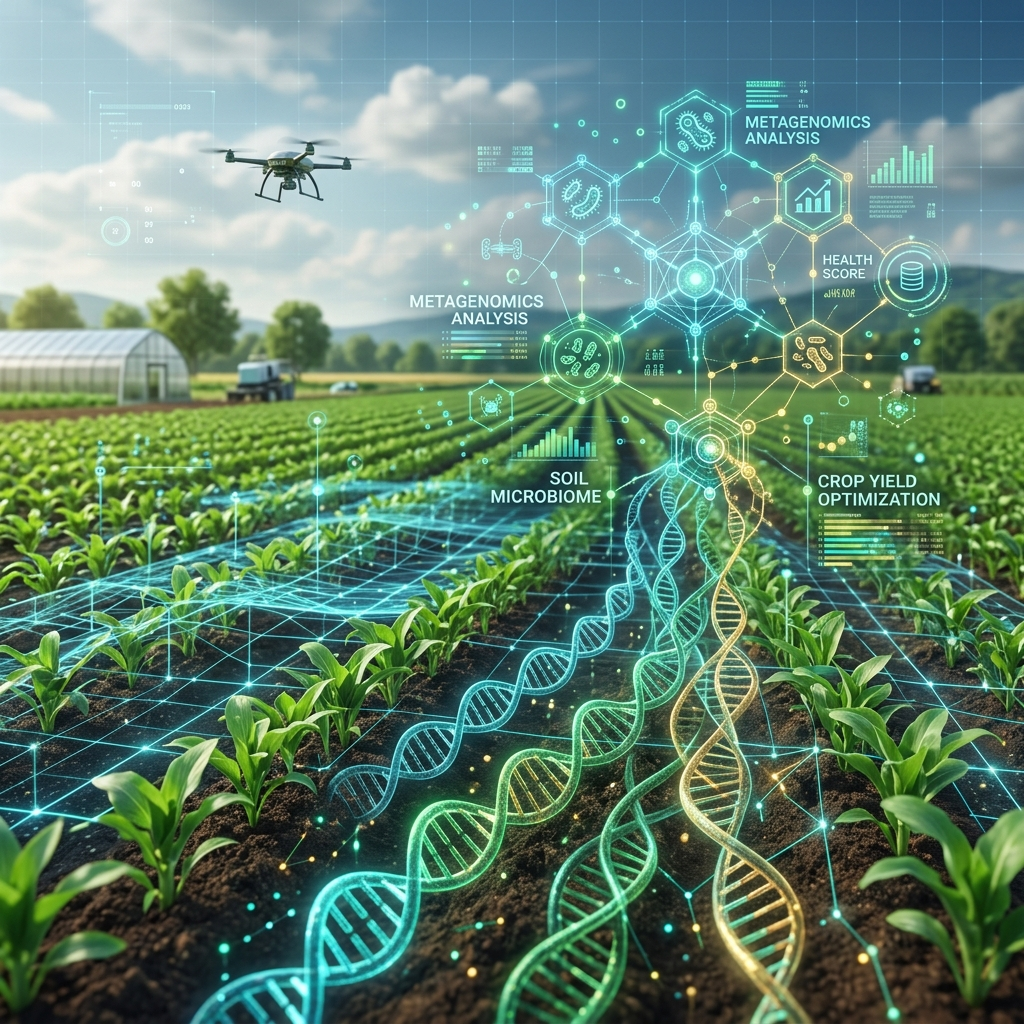
\includegraphics[width=0.85\textwidth]{assets/ch09_metagenomics_ai.png}
    \caption{การจำลอง 3D แสดงขั้นตอนการสกัด DNA จากดินไรโซสเฟียร์ การถอดรหัสพันธุกรรมเมตาเจโนมิกส์ และการวิเคราะห์เครือข่ายสังคมจุลินทรีย์ดิน (Microbial Network) ด้วยซอฟต์แวร์ชีวสารสนเทศศาสตร์ เพื่อคัดเลือกสายพันธุ์หลัก (Hub taxa) สู่การสร้างกลุ่มจุลินทรีย์สังเคราะห์}
    \label{fig:ch09_metagenomics_ai}
\end{figure}

\section*{วัตถุประสงค์การเรียนรู้ประจำบท}
เมื่อศึกษาบทเรียนนี้จบแล้ว นักศึกษาสามารถ:
\begin{enumerate}
    \item เปรียบเทียบข้อแตกต่างเชิงเทคนิคระหว่าง 16S/ITS Amplicon Sequencing และ Whole Metagenome Shotgun (WGS)
    \item วิเคราะห์ขั้นตอนการทำงานของไปป์ไลน์ชีวสารสนเทศศาสตร์มาตรฐาน (FastQC $\rightarrow$ Trimmomatic $\rightarrow$ DADA2 $\rightarrow$ QIIME2)
    \item คำนวณและแปลผลดัชนีความหลากหลายระดับท้องถิ่น (Alpha Diversity: Shannon, Simpson, Chao1) และความแตกต่างระหว่างกลุ่ม (Beta Diversity: Bray-Curtis, UniFrac)
    \item อธิบายหลักการวิเคราะห์เครือข่ายสังคมจุลินทรีย์ (Co-occurrence Networks) และการระบุชนิดพันธุ์ศูนย์กลาง (Keystone Hub Taxa)
    \item ออกแบบสูตรกลุ่มจุลินทรีย์สังเคราะห์ (SynComs) จากการบูรณาการข้อมูลเมตาเจโนมิกส์เพื่อแก้ปัญหาดินเหนียวแน่นและโรคระบาดในแปลงเกษตร
\end{enumerate}

\section{เทคโนโลยีถอดรหัสพันธุกรรมเมตาเจโนมิกส์ในดินเกษตร}

การศึกษาจุลินทรีย์ดินในยุคปัจจุบันแบ่งออกเป็น 2 แนวทางหลักตามระดับความลึกของข้อมูล:

\subsection{1. การจัดทำโพรไฟล์ยีนเครื่องหมาย (Amplicon Targeted Sequencing)}
เป็นการเพิ่มปริมาณยีนเป้าหมายที่มีบริเวณอนุรักษ์ (Conserved regions) สลับกับบริเวณที่มีความผันแปรสูง (Hypervariable regions) ด้วยเทคนิค PCR ก่อนส่งตรวจ NGS:
\begin{itemize}
    \item \textbf{แบคทีเรียและอาร์เคีย:} นิยมใช้ยีน \textbf{16S rRNA\index{16S rRNA gene sequencing}} โดยเฉพาะบริเวณผันแปร $V3-V4$ หรือ $V4$ ขนาดประมาณ 250--460 คู่เบส ซึ่งมีฐานข้อมูลอ้างอิงระดับโลก เช่น SILVA และ Greengenes
    \item \textbf{เชื้อราในดิน:} นิยมใช้บริเวณ \textbf{Internal Transcribed Spacer (ITS)\index{Internal Transcribed Spacer (ITS)}} ได้แก่ ITS1 หรือ ITS2 ซึ่งแทรกอยู่ระหว่างยีน 18S, 5.8S, และ 28S rRNA โดยเทียบกับฐานข้อมูล UNITE
\end{itemize}

\subsection{2. ช็อตกันเมตาเจโนมิกส์ทั้งชุมชน (Whole Metagenome Shotgun: WGS)}
เป็นการสกัด DNA ทั้งหมดในตัวอย่างดิน ตัดชิ้นส่วนให้สั้นลง แล้วหาลำดับเบสพร้อมกันทั้งหมดโดยไม่ผ่านการเพิ่มขยายยีนด้วย PCR (PCR-free):\index{Whole Metagenome Shotgun (WGS)}
\begin{itemize}
    \item ให้ข้อมูลทั้งโครงสร้างชนิดพันธุ์ (Taxonomic profiling) และข้อมูลหน้าที่ของยีนทั้งระบบ (Functional profiling) เช่น ยีนสร้างเอนไซม์ไนโตรจีเนส (\textit{nifH}), ยีนละลายฟอสเฟต (\textit{phoD}), หรือยีนสร้างยาปฏิชีวนะ (NRPS/PKS)
    \item สามารถนำชิ้นส่วนเบสมาต่อกัน (De novo assembly) จนได้จีโนมจุลินทรีย์ที่สมบูรณ์จากสิ่งแวดล้อม เรียกว่า **Metagenome-Assembled Genomes (MAGs)** แม้จะไม่เคยเพาะเลี้ยงเชื้อนั้นได้มาก่อน
\end{itemize}

\section{เวิร์กโฟลว์ชีวสารสนเทศศาสตร์: จากข้อมูลดิบสู่ ASVs}

\begin{figure}[ht]
\centering
\begin{tikzpicture}[node distance=1.5cm, auto,
    block/.style={rectangle, draw, fill=blue!10, text width=10.0cm, rounded corners, minimum height=0.9cm, align=left},
    arrow/.style={thick, ->, >=stealth}]
    
    \node [block] (step1) {\textbf{1. Raw FastQ Reads:} ตรวจสอบคุณภาพด้วย FastQC และ MultiQC};
    \node [block, below of=step1] (step2) {\textbf{2. Preprocessing:} ตัดไพรเมอร์ด้วย Cutadapt และกรองเบสคุณภาพต่ำด้วย Trimmomatic};
    \node [block, below of=step2] (step3) {\textbf{3. Denoising (DADA2):} สร้างโมเดลความคลาดเคลื่อนเบส แยกความแปรผันทางชีววิทยาออกจาก Noise ได้ตาราง Amplicon Sequence Variants (ASVs) ที่ความละเอียดระดับ 1 นิวคลีโอไทด์};
    \node [block, below of=step3] (step4) {\textbf{4. Chimera Removal:} ตรวจจับและกำจัดสายผสมไคเมรา};
    \node [block, below of=step4] (step5) {\textbf{5. QIIME2 Pipeline:} ระบุอนุกรมวิธานด้วย Naive Bayes Classifier เทียบฐานข้อมูล SILVA/UNITE และสร้างแผนภูมิต้นไม้ไฟโลเจเนติก};
    
    \draw [arrow] (step1) -- (step2);
    \draw [arrow] (step2) -- (step3);
    \draw [arrow] (step3) -- (step4);
    \draw [arrow] (step4) -- (step5);
\end{tikzpicture}
\caption{เวิร์กโฟลว์การประมวลผลข้อมูลชีวสารสนเทศศาสตร์เมตาเจโนมิกส์ด้วย DADA2 และ QIIME2}
\label{fig:bioinfo_pipeline}
\end{figure}

ในอดีต นักชีวสารสนเทศศาสตร์นิยมจัดกลุ่มลำดับเบสที่มีความเหมือนกัน $97\%$ ให้เป็นหนึ่งหน่วย Operational Taxonomic Unit (OTU) แต่วิธีนี้มีความคลาดเคลื่อนสูงและซ่อนความแตกต่างระดับสายพันธุ์ ในปัจจุบัน วงการวิจัยสากลได้เปลี่ยนมาใช้ **Amplicon Sequence Variants (ASVs)** ซึ่งพัฒนาโดย Callahan และคณะ (2016) \cite{callahan2016dada2} ร่วมกับแพลตฟอร์ม QIIME2 \cite{bolyen2019qiime2}:
\begin{itemize}
    \item อัลกอริทึม DADA2 ใช้แบบจำลองความน่าจะเป็นตามสถิติของเครื่องซีเควนเซอร์ เพื่อตัดสัญญาณรบกวน (Denoising) ทำให้สามารถแยกความแตกต่างของสายพันธุ์ที่มีลำดับเบสต่างกันเพียงตัวเดียว ($1\text{ bp difference}$) ได้อย่างแม่นยำ
    \item ข้อมูล ASVs เป็นค่าสัมบูรณ์ที่มีความเที่ยงตรงสูง สามารถนำตาราง ASVs จากการทดลองต่างสถานที่หรือต่างช่วงเวลามาเปรียบเทียบข้ามชุดข้อมูลกันได้โดยตรง
\end{itemize}

\section{ดัชนีชี้วัดความหลากหลายทางนิเวศวิทยาของจุลินทรีย์ดิน}

\subsection{1. ดัชนีความหลากหลายภายในแหล่งอาศัย (Alpha Diversity)}
ประเมินความหลากหลายและความสม่ำเสมอของประชากรจุลินทรีย์ภายในตัวอย่างดินหนึ่งๆ:\index{ความหลากหลายของสายพันธุ์ (Alpha Diversity)}
\begin{itemize}
    \item \textbf{Richness ($S$):} จำนวนชนิดหรือจำนวน ASVs ทั้งหมดที่ตรวจพบ
    \item \textbf{Shannon Diversity Index ($H'$):\index{Shannon Diversity Index ($H'$)}} วัดทั้งความหลากหลายของชนิดพันธุ์และความสม่ำเสมอ (Evenness) ในการกระจายตัว:
    \begin{equation}
    H' = - \sum_{i=1}^{S} p_i \ln(p_i)
    \end{equation}
    เมื่อ $p_i = n_i / N$ คือสัดส่วนความหนาแน่นสัมพัทธ์ของ ASV ลำดับที่ $i$
    \item \textbf{Simpson's Diversity Index ($D$ และ $1/D$):\index{Simpson's Diversity Index}} วัดความน่าจะเป็นที่เมื่อสุ่มเลือกจุลินทรีย์ 2 ตัวขึ้นมาแล้วจะพบว่าเป็นชนิดเดียวกัน:
    \begin{equation}
    D = \sum_{i=1}^{S} p_i^2 \quad \implies \quad \text{Inverse Simpson} = \frac{1}{D} = \frac{1}{\sum p_i^2}
    \end{equation}
    \item \textbf{Chao1 Estimator:\index{Chao1 Estimator}} ตัวประมาณการความหลากหลายที่แท้จริง โดยคำนึงถึงชนิดพันธุ์ที่พบน้อย (Rare taxa) ทั้งที่พบเพียงครั้งเดียว ($F_1$: Singletons) และพบสองครั้ง ($F_2$: Doubletons):
    \begin{equation}
    S_{\text{Chao1}} = S_{\text{obs}} + \frac{F_1 (F_1 - 1)}{2 (F_2 + 1)}
    \end{equation}
\end{itemize}

\subsection{2. ดัชนีความแตกต่างระหว่างแหล่งอาศัย (Beta Diversity)}
ประเมินความแตกต่างของโครงสร้างชุมชนจุลินทรีย์ระหว่างตัวอย่างดินต่างกรรมวิธี (เช่น ดินเกษตรอินทรีย์ vs ดินเกษตรเคมี):\index{Beta Diversity}
\begin{itemize}
    \item \textbf{Bray-Curtis Dissimilarity ($BC_{jk}$):\index{Bray-Curtis Dissimilarity}} คำนึงถึงความหนาแน่นสัมพัทธ์ของแต่ละชนิด:
    \begin{equation}
    BC_{jk} = \frac{\sum_{i=1}^{S} |n_{ij} - n_{ik}|}{\sum_{i=1}^{S} (n_{ij} + n_{ik})} = 1 - \frac{2 C_{jk}}{S_j + S_k}
    \end{equation}
    ค่า $BC = 0$ หมายถึงชุมชนจุลินทรีย์เหมือนกันทุกประการ และ $BC = 1$ หมายถึงไม่มีสปีชีส์ใดร่วมกันเลย
    \item \textbf{UniFrac Distance (Weighted / Unweighted):} ดัชนีที่บูรณาการความสัมพันธ์ทางสายวิวัฒนาการ (Phylogenetic distance) บนต้นไม้สายสัมพันธ์เข้าด้วยกัน
\end{itemize}

\section{เครือข่ายสังคมจุลินทรีย์และกลุ่มจุลินทรีย์สังเคราะห์ (SynComs)}

ในสภาพแวดล้อมดิน จุลินทรีย์ไม่ได้อาศัยอยู่อย่างโดดเดี่ยว แต่เชื่อมโยงกันเป็นเครือข่ายปฏิสัมพันธ์ (Co-occurrence Network):\index{เครือข่ายสังคมจุลินทรีย์ (Co-occurrence Networks)}

\subsection{1. การวิเคราะห์โครงสร้างเครือข่าย (Network Topologies)}
การใช้สถิติสหสัมพันธ์แบบ Spearman หรือ Sparse Correlations for Compositional Data (SparCC) ช่วยระบุความสัมพันธ์:
\begin{itemize}
    \item \textbf{Positive Edge (ขอบบวก):} แสดงถึงการเกื้อกูลกัน การใช้อาหารร่วมกัน (Syntrophy) หรือการอยู่อาศัยในถิ่นอาศัยเดียวกัน
    \item \textbf{Negative Edge (ขอบลบ):} แสดงถึงการแก่งแย่งแข่งขันสารอาหาร (Competition) หรือการสร้างสารปฏิชีวนะยับยั้งกัน (Amensalism)
    \item \textbf{Keystone Hub Taxa (ชนิดพันธุ์แกนหลัก):\index{Keystone Hub Taxa}} จุลินทรีย์ที่มีค่า Degree Centrality และ Closeness Centrality สูงมาก หากกำจัดจุลินทรีย์แกนหลักเหล่านี้ออก เครือข่ายไมโครไบโอมในดินจะพังทลายลงทันที
\end{itemize}

\subsection{2. การออกแบบกลุ่มจุลินทรีย์สังเคราะห์ (Synthetic Communities: SynComs)}
Vorholt และคณะ (2017) \cite{vorholt2017syncom} ได้วางกรอบแนวคิดการสร้าง \textbf{SynComs\index{กลุ่มจุลินทรีย์สังเคราะห์ (SynComs)}} ซึ่งเป็นการคัดเลือกจุลินทรีย์ที่เพาะเลี้ยงได้จำนวนหนึ่ง (ปกติ 5--20 สายพันธุ์) ที่มีหน้าที่ทางชีวเคมีเกื้อหนุนกันตามข้อมูลเมตาเจโนมิกส์:
\begin{enumerate}
    \item สายพันธุ์ที่ 1: ตรึงไนโตรเจน (\organism{Azospirillum brasilense})
    \item สายพันธุ์ที่ 2: ละลายฟอสเฟต (\organism{Bacillus velezensis})
    \item สายพันธุ์ที่ 3: สังเคราะห์สารไซเดอโรฟอร์จับเหล็ก (\organism{Pseudomonas putida})
    \item สายพันธุ์ที่ 4: ผลิตเอนไซม์ ACC Deaminase ลดความเครียดพืช
    \item สายพันธุ์ที่ 5: ป้องกันเชื้อราก่อโรคด้วยสารไลโปเปปไทด์
\end{enumerate}
การรวมกลุ่มแบบ SynComs ช่วยแก้ปัญหาความล้มเหลวของการใช้หัวเชื้อเดี่ยว (Single-strain inoculant) ในแปลงเกษตรจริงได้อย่างยั่งยืน

\begin{application}[กรณีศึกษางานวิจัย RBRU: การวิเคราะห์ 16S Amplicon Metagenomics ในสวนทุเรียน จ.จันทบุรี]
จากงานวิจัยของ Jantamalee \& Thassana (2025) \cite{jantamalee_2025} ณ มหาวิทยาลัยราชภัฏรำไพพรรณี\index{งานวิจัย RBRU!16S Metagenomics สวนทุเรียน} ได้ดำเนินการสกัด Soil DNA และถอดรหัสลำดับเบสบริเวณยีน 16S rRNA (V3--V4 region) ด้วยเทคโนโลยี Illumina NovaSeq 6000 ในดินไรโซสเฟียร์สวนทุเรียนพันธุ์หมอนทอง 2 กลุ่มจัดการ ได้แก่ แปลงเกษตรอินทรีย์ชีวภาพ (อ.เขาคิชฌกูฏ) และแปลงเกษตรเคมีเข้มข้น (อ.ท่าใหม่):
\begin{itemize}
    \item \textbf{Alpha Diversity:} แปลงเกษตรอินทรีย์มีค่า Shannon Index สูงถึง $H' = 4.86 \pm 0.14$ และ Chao1 $= 1,420$ เทียบกับแปลงเกษตรเคมีที่พบเพียง $H' = 3.18 \pm 0.22$ และ Chao1 $= 780$ แสดงถึงการสูญเสียความหลากหลายอย่างรุนแรงจากการใช้สารเคมีต่อเนื่อง
    \item \textbf{Taxonomic Profiling:} ดินอินทรีย์อุดมไปด้วยไฟลัม \textit{Firmicutes} (สกุล \organism{Bacillus}) และ \textit{Actinobacteria} (สกุล \organism{Streptomyces}) ในสัดส่วนรวมกันมากกว่าร้อยละ 45 ขณะที่แปลงเคมีมีสัดส่วนของ \textit{Proteobacteria} ฉวยโอกาสเพิ่มขึ้น
    \item \textbf{Co-occurrence Network:} การวิเคราะห์เครือข่ายระบุว่า \organism{Bacillus velezensis} และ \organism{Bradyrhizobium} ทำหน้าที่เป็น Keystone Hub Taxa สำคัญ ซึ่งเป็นฐานข้อมูลชีวภาพในการสังเคราะห์กลุ่มจุลินทรีย์ SynComs ท้องถิ่น
\end{itemize}
\end{application}

\begin{worked}[ตัวอย่างที่ 9.1 การคำนวณ Shannon Index และ Simpson Index ของดินแปลงทุเรียน]
จากการวิเคราะห์ 16S rRNA sequencing พบสัดส่วนจำนวนนับของแบคทีเรีย 5 กลุ่มหลักในดินแปลงเกษตรอินทรีย์ที่มีสุขภาพดี:
\begin{center}
\small
\begin{tabular}{lcc}
\toprule
\textbf{กลุ่มแบคทีเรียหลัก} & \textbf{จำนวนนับ (Reads: $n_i$)} & \textbf{สัดส่วนสัมพัทธ์ ($p_i$)} \\
\midrule
1. \textit{Acidobacteria} & 3,200 & 0.32 \\
2. \textit{Actinobacteria} & 2,500 & 0.25 \\
3. \textit{Proteobacteria} & 2,100 & 0.21 \\
4. \textit{Firmicutes} & 1,400 & 0.14 \\
5. \textit{Bacteroidetes} & 800 & 0.08 \\
\midrule
\textbf{รวม ($N$)} & \textbf{10,000} & \textbf{1.00} \\
\bottomrule
\end{tabular}
\end{center}

จงคำนวณค่า Shannon Diversity Index ($H'$) และ Inverse Simpson Index ($1/D$) ของตัวอย่างดินนี้

\textbf{วิธีทำ:}
1. คำนวณค่า $p_i \ln(p_i)$ ของแต่ละกลุ่ม:
\begin{itemize}
    \item กลุ่ม 1: $0.32 \times \ln(0.32) = 0.32 \times (-1.1394) \approx -0.3646$
    \item กลุ่ม 2: $0.25 \times \ln(0.25) = 0.25 \times (-1.3863) \approx -0.3466$
    \item กลุ่ม 3: $0.21 \times \ln(0.21) = 0.21 \times (-1.5606) \approx -0.3277$
    \item กลุ่ม 4: $0.14 \times \ln(0.14) = 0.14 \times (-1.9661) \approx -0.2753$
    \item กลุ่ม 5: $0.08 \times \ln(0.08) = 0.08 \times (-2.5257) \approx -0.2021$
\end{itemize}
$$\sum p_i \ln(p_i) = -0.3646 - 0.3466 - 0.3277 - 0.2753 - 0.2021 = -1.5163$$
$$H' = -(-1.5163) \approx 1.5163$$

2. คำนวณค่า Simpson Index ($D = \sum p_i^2$):
$$D = (0.32)^2 + (0.25)^2 + (0.21)^2 + (0.14)^2 + (0.08)^2$$
$$D = 0.1024 + 0.0625 + 0.0441 + 0.0196 + 0.0064 = 0.2350$$
$$\text{Inverse Simpson } (1/D) = \frac{1}{0.2350} \approx 4.255$$

\textbf{บทวิเคราะห์ผลลัพธ์:} ค่า Shannon Index เท่ากับ 1.5163 และ Inverse Simpson เท่ากับ 4.255 บ่งชี้ว่าดินในแปลงอินทรีย์นี้มีการกระจายตัวของกลุ่มจุลินทรีย์ที่สม่ำเสมอดีมาก ไม่มีกลุ่มใดครอบงำ (Dominance) จนทำลายความหลากหลาย ซึ่งเป็นลักษณะโครงสร้างดินที่ต้านทานการเกิดโรคพืชได้ดี
\end{worked}

\begin{worked}[ตัวอย่างที่ 9.2 การคำนวณ Bray-Curtis Dissimilarity เปรียบเทียบดินสองกรรมวิธี]
นักวิจัยเก็บตัวอย่างดินจากแปลงเกษตรอินทรีย์ ($j$) และแปลงเกษตรเคมีเข้มข้น ($k$) ตรวจนับ ASVs เด่น 4 ชนิด:

\begin{center}
\small
\begin{tabular}{cccc}
\toprule
\textbf{ชนิด ASV เด่น} & \textbf{แปลงอินทรีย์ ($n_{ij}$)} & \textbf{แปลงเคมี ($n_{ik}$)} & \textbf{ผลต่าง $|n_{ij} - n_{ik}|$} \\
\midrule
ASV 1 (\textit{Rhizobium}) & 120 & 20 & 100 \\
ASV 2 (\textit{Bacillus}) & 85 & 35 & 50 \\
ASV 3 (\textit{Nitrosomonas}) & 40 & 15 & 25 \\
ASV 4 (\textit{Fusarium}) & 10 & 90 & 80 \\
\midrule
\textbf{รวม} & \textbf{255} & \textbf{160} & \textbf{255} \\
\bottomrule
\end{tabular}
\end{center}

จงคำนวณดัชนีความไม่เหมือน Bray-Curtis Dissimilarity ($BC_{jk}$) ระหว่างสองแปลงนี้

\textbf{วิธีทำ:}
$$BC_{jk} = \frac{\sum |n_{ij} - n_{ik}|}{\sum (n_{ij} + n_{ik})}$$
$$\sum |n_{ij} - n_{ik}| = 100 + 50 + 25 + 80 = 255$$
$$\sum (n_{ij} + n_{ik}) = 255 + 160 = 415$$
$$BC_{jk} = \frac{255}{415} \approx 0.6145 \text{ หรือ } 61.45\%$$

\textbf{บทวิเคราะห์ผลลัพธ์:} ค่าความไม่เหมือน Bray-Curtis เท่ากับ $61.45\%$ บ่งชี้ว่าการใช้สารเคมีส่งผลกระทบอย่างรุนแรงต่อโครงสร้างของไมโครไบโอมดิน ทำให้กลุ่มแบคทีเรียที่เป็นประโยชน์ (\textit{Rhizobium}, \textit{Bacillus}) ลดลงอย่างมีนัยสำคัญ ในขณะที่เชื้อราก่อโรคพืช (\textit{Fusarium}) เพิ่มขึ้นถึง 9 เท่า
\end{worked}

% [RESEARCH-UPDATE-2026-10]
\section{ความก้าวหน้างานวิจัยล่าสุดด้านเมตาเจโนมิกส์ทางการเกษตร}

งานวิจัยระดับแนวหน้าในปี ค.ศ. 2024–2026 โดย Clagnan และคณะ \cite{pmid39526137} ได้ผสานเทคนิคคัลเชอโรมิกส์ (Culturomics: การเพาะเลี้ยงนับร้อยสภาวะ) ร่วมกับเมตาเจโนมิกส์ความลึกสูง พบว่าการฟื้นฟูดินด้วยหัวเชื้อจุลินทรีย์สังเคราะห์ SynComs สามารถเพิ่มความอุดมสมบูรณ์ของยีนหมุนเวียนคาร์บอนและไนโตรเจนในดินที่เสื่อมโทรมได้อย่างรวดเร็ว

ในขณะเดียวกัน งานวิจัยของ Panek และคณะ \cite{pmid41800415} ได้แสดงให้เห็นว่าการวิเคราะห์เครื่องหมายเมตาเจโนมิกส์ (Metagenomic Biomarkers) สามารถใช้เป็นดัชนีเตือนภัยล่วงหน้า (Early-Warning Biomarkers) ของการพังทลายของระบบนิเวศดินก่อนที่ค่าทางเคมีกายภาพ (pH, N-P-K) จะเปลี่ยนแปลงถึง 1 ฤดูปลูก

\begin{insight}[ประเด็นวิเคราะห์เชิงวิชาการ]
เหตุใดการศึกษาความหลากหลายทางชีวภาพของแบคทีเรียในดิน จึงไม่ควรยึดติดอยู่กับลำดับเบส 16S rRNA เพียงอย่างเดียว? และข้อมูล Shotgun Metagenomics มีข้อได้เปรียบอย่างไรในการศึกษาบทบาทเชิงฟังก์ชันของยีนต้านทานยาปฏิชีวนะ (ARGs) ในดินเกษตรกรรม?
\end{insight}

\section*{สรุปประจำบท}

เทคโนโลยีเมตาเจโนมิกส์และชีวสารสนเทศศาสตร์ได้ปฏิวัติความเข้าใจเกี่ยวกับไมโครไบโอมในดินอย่างสิ้นเชิง การเปลี่ยนผ่านจากเทคนิคการเพาะเลี้ยงแบบเดิมสู่การถอดรหัสพันธุกรรมขั้นสูงทั้ง Amplicon Sequencing (ยีน 16S rRNA และบริเวณ ITS) และ Whole Metagenome Shotgun ร่วมกับไปป์ไลน์ DADA2 และ QIIME2 ช่วยให้นักวิจัยเข้าถึงความหลากหลายระดับ ASVs ได้อย่างแม่นยำ การคำนวณดัชนี Alpha Diversity (Shannon, Simpson, Chao1) และ Beta Diversity (Bray-Curtis, UniFrac) ช่วยประเมินความสมบูรณ์และเสถียรภาพของดินได้อย่างเป็นรูปธรรม ยิ่งไปกว่านั้น การทำความเข้าใจโครงสร้างเครือข่ายสังคมจุลินทรีย์และการระบุชนิดพันธุ์แกนหลัก (Hub taxa) ถือเป็นรากฐานสำคัญสู่การสร้างกลุ่มจุลินทรีย์สังเคราะห์ (SynComs) ที่ช่วยฟื้นฟูระบบนิเวศการเกษตรได้อย่างตรงจุดและยั่งยืน

\subsection*{คำถามท้ายบทและการวิเคราะห์}

\noindent \textbf{ระดับที่ 1: ความรู้และความเข้าใจเชิงทฤษฎี (Knowledge \& Comprehension)}
\begin{enumerate}
    \item เปรียบเทียบข้อดีและข้อจำกัดระหว่างการวิเคราะห์ Amplicon Sequencing (16S/ITS) กับการวิเคราะห์ Whole Metagenome Shotgun (WGS)
    \item อธิบายความแตกต่างพื้นฐานระหว่างหน่วย Operational Taxonomic Units (OTUs ที่ 97\%) กับ Amplicon Sequence Variants (ASVs) ในการวิเคราะห์ชีวสารสนเทศศาสตร์
    \item เหตุใดบริเวณยีน 16S rRNA จึงได้รับการคัดเลือกให้เป็นยีนเครื่องหมายสากลสำหรับการจัดจำแนกแบคทีเรียและอาร์เคีย?
    \item สรุปขั้นตอนการทำงานของไปป์ไลน์ชีวสารสนเทศศาสตร์มาตรฐานตั้งแต่ Raw Reads (FastQ) จนถึงการได้ตาราง ASVs ในซอฟต์แวร์ DADA2
\end{enumerate}

\noindent \textbf{ระดับที่ 2: การวิเคราะห์และการคำนวณเชิงปริมาณ (Quantitative Analysis \& Calculation)}
\begin{enumerate}[resume]
    \item อธิบายความหมายเชิงนิเวศวิทยาของดัชนี Shannon Diversity Index ($H'$) และเปรียบเทียบกับดัชนี Simpson's Index ($D$)
    \item ในการคำนวณความหลากหลาย Chao1 ตัวแปร Singletons ($F_1$) และ Doubletons ($F_2$) มีความสำคัญต่อการประมาณจำนวนชนิดพันธุ์ทั้งหมดอย่างไร?
    \item ในแปลงปลูกส้มมี ASVs ของแบคทีเรีย 3 ชนิด ด้วยจำนวนนับ $n_1 = 500$, $n_2 = 300$, และ $n_3 = 200$ จงคำนวณหาค่า Shannon Index ($H'$)
\end{enumerate}

\noindent \textbf{ระดับที่ 3: การสังเคราะห์และการแก้ปัญหาในแปลงจริง (Application \& Real-World Synthesis)}
\begin{enumerate}[resume]
    \item ดัชนี Bray-Curtis Dissimilarity ใช้วัดสิ่งใด และค่าที่ได้มีความหมายอย่างไรเมื่อเปรียบเทียบแปลงเกษตรอินทรีย์กับแปลงเกษตรเคมี?
    \item จากกรณีศึกษางานวิจัย RBRU ในสวนทุเรียน จ.จันทบุรี จงอธิบายบทบาทของ Keystone Hub Taxa ต่อเสถียรภาพของไมโครไบโอมดิน และเหตุใดการใช้สารเคมีต่อเนื่องจึงทำให้ค่า Shannon Index ลดลง?
    \item จงออกแบบขั้นตอนการคัดเลือกและทดสอบกลุ่มจุลินทรีย์สังเคราะห์ (Synthetic Communities: SynComs) จำนวน 6 สายพันธุ์ เพื่อใช้ฟื้นฟูดินเค็มและส่งเสริมการเจริญเติบโตของข้าว
\end{enumerate}

\chapter{สถาปัตยกรรม AIoT วิทัศน์คอมพิวเตอร์ และเกษตรแม่นยำสำหรับไมโครไบโอม}
\label{ch:aiot_precision}

\begin{keyconcept}[แนวคิดสำคัญของบทที่ 10]
การปฏิวัติการเกษตรสู่ยุคดิจิทัล (Agriculture 4.0/5.0) ก้าวข้ามจากการตรวจวัดค่าเคมีกายภาพแบบแยกส่วน สู่การเชื่อมโยงระบบโทรมาตรภาคสนาม (Field Telemetry)\index{โทรมาตรแปลงเกษตร (Field Telemetry)} เข้ากับพลวัตของไมโครไบโอมดินและสรีรวิทยาพืชผ่านสถาปัตยกรรม \textbf{AIoT (Artificial Intelligence of Things)\index{AIoT (Artificial Intelligence of Things)}} การบูรณาการเซนเซอร์ดินอเนกประสงค์ (RS485 Modbus RTU 7-in-1)\index{โพรโทคอล Modbus RTU}\index{RS485 Differential Signaling} ร่วมกับไมโครคอนโทรลเลอร์ ESP32\index{ESP32-S3 Microcontroller} และเครือข่ายสัญญาณระยะไกล LoRaWAN\index{LoRaWAN (Long Range Wide Area Network)} ทำให้สามารถติดตามความชื้น อุณหภูมิ ดัชนีการนำไฟฟ้า (EC) และสารอาหารดินแบบเรียลไทม์ ขณะเดียวกัน การประยุกต์ใช้โมเดลวิทัศน์คอมพิวเตอร์ขนาดย่อมเยา (Edge AI: YOLOv8-Nano, MobileNetV4)\index{การตรวจจำแนกโรคพืชด้วย Edge AI}\index{YOLOv8-Nano Deep Learning}\index{MobileNetV4} และอัลกอริทึมการเรียนรู้ของเครื่อง (Machine Learning: Random Forest)\index{Random Forest Regression} ช่วยให้สามารถประเมินดัชนีความรุนแรงของโรคพืชและควบคุมการปล่อยชีวภัณฑ์ PGPR แบบแปรผันตามพื้นที่จริงได้อย่างแม่นยำ
\end{keyconcept}

\begin{figure}[ht]
    \centering
    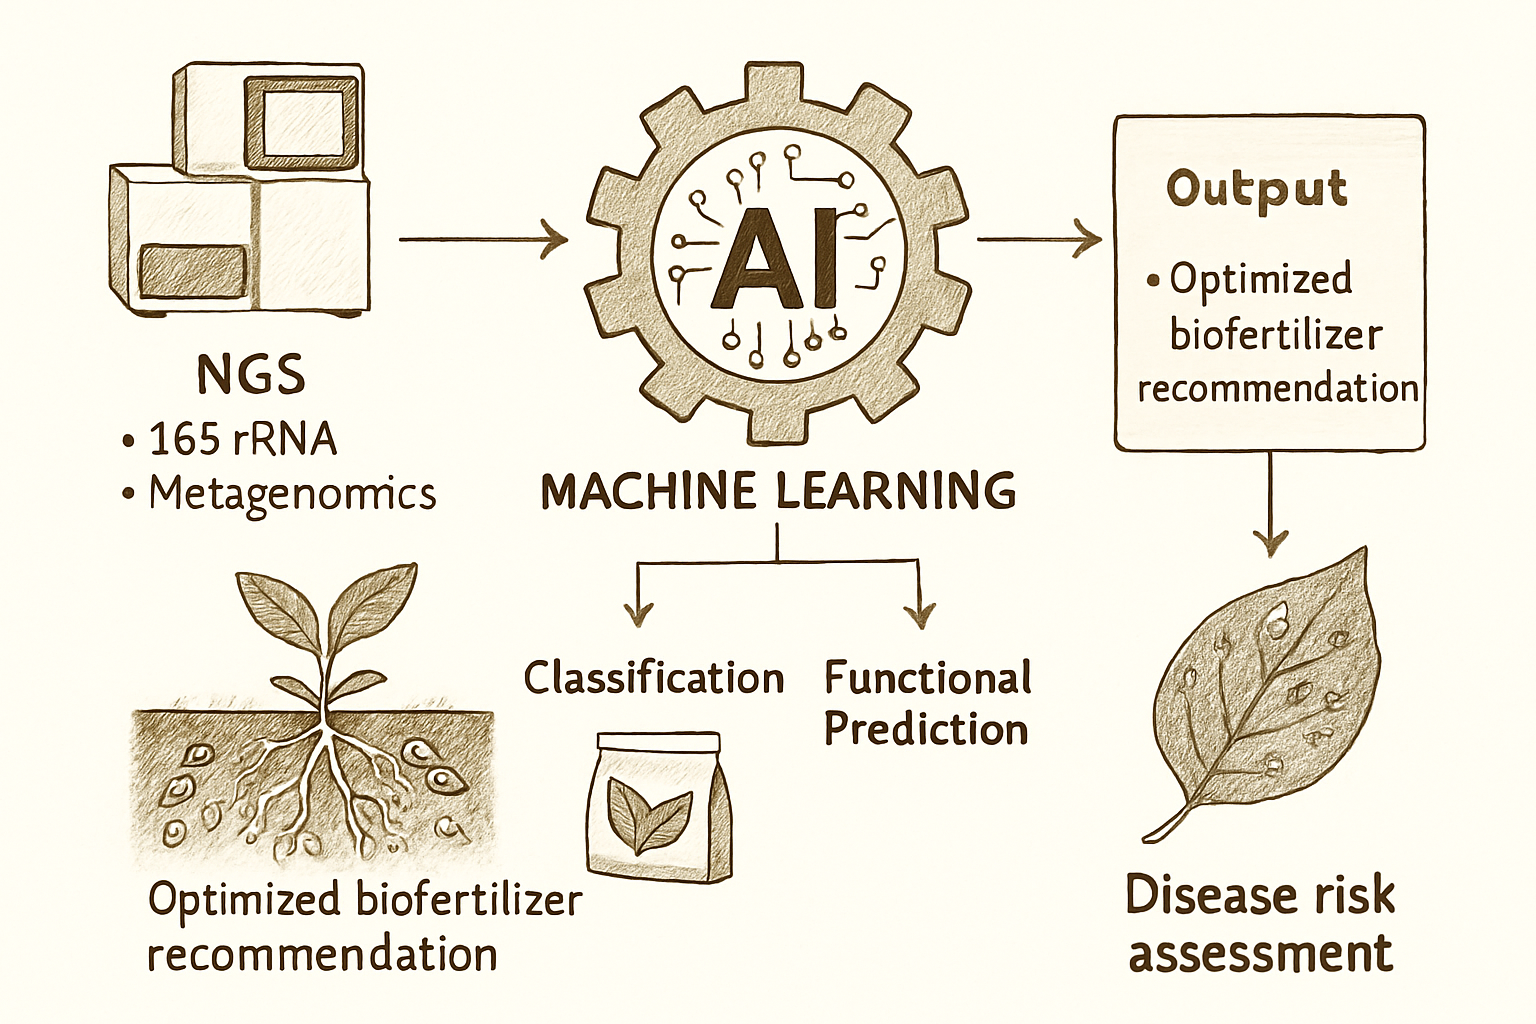
\includegraphics[width=0.85\textwidth]{assets/ch10_ai_telemetry.png}
    \caption{สถาปัตยกรรมระบบนิเวศ AIoT ในแปลงเกษตรอัจฉริยะ แสดงเซนเซอร์ดิน RS485 Modbus RTU โหนดประมวลผลไมโครคอนโทรลเลอร์ ESP32 การส่งผ่านข้อมูลด้วยสัญญาณ LoRaWAN เข้าสู่แดชบอร์ดคลาวด์ และโมเดล Edge AI ตรวจจำแนกโรคพืชและควบคุมการฉีดพ่นชีวภัณฑ์อัตโนมัติ}
    \label{fig:ch10_aiot_architecture}
\end{figure}

\section*{วัตถุประสงค์การเรียนรู้ประจำบท}
เมื่อศึกษาบทเรียนนี้จบแล้ว นักศึกษาสามารถ:
\begin{enumerate}
    \item อธิบายสถาปัตยกรรมระบบโทรมาตร AIoT และโปรโตคอลการสื่อสารอุตสาหกรรม RS485 Modbus RTU สำหรับเซนเซอร์ดิน
    \item ถอดรหัสโครงสร้างเฟรมข้อมูลฐานสิบหก (Hexadecimal Frame) และการคำนวณรหัสตรวจสอบความถูกต้อง CRC16 ของเซนเซอร์ดิน
    \item วิเคราะห์การประยุกต์ใช้อัลกอริทึมการเรียนรู้ของเครื่อง (Random Forest / LightGBM) เพื่อสร้างแบบจำลองทำนายพลวัตของจุลินทรีย์ในดิน
    \item อธิบายสถาปัตยกรรมโครงข่ายประสาทเทียมแบบขนาดย่อมเยา (Lightweight Edge AI: YOLOv8-Nano, MobileNetV4) สำหรับการตรวจจับโรคพืช
    \item คำนวณเมทริกซ์ความสับสน (Confusion Matrix) ค่าความแม่นยำ (Precision) ความระลึก (Recall) และ F1-Score ของโมเดลจำแนกโรคพืช
\end{enumerate}

\section{สถาปัตยกรรมฮาร์ดแวร์และโทรมาตร AIoT ในแปลงเกษตร}

ระบบฟาร์มอัจฉริยะที่เชื่อมโยงกับชีววิทยาของจุลินทรีย์ดิน ประกอบด้วยโครงสร้างพื้นฐานทางวิศวกรรม 4 ระดับชั้น (4-Tier Architecture):

\begin{figure}[ht]
\centering
\begin{tikzpicture}[node distance=1.6cm, auto,
    layer/.style={rectangle, draw, fill=teal!15, text width=10.5cm, rounded corners, minimum height=1.0cm, align=left},
    arrow/.style={thick, <->, >=stealth}]
    
    \node [layer] (l1) {\textbf{1. Perception Layer (ชั้นตรวจวัด):} หัววัดดิน 7-in-1 (RS485 Modbus RTU), กล้องตรวจการณ์ Multispectral, เซนเซอร์สภาพอากาศ microclimate};
    \node [layer, below of=l1] (l2) {\textbf{2. Edge Computing Layer (ชั้นประมวลผลปลายทาง):} ไมโครคอนโทรลเลอร์ ESP32-S3, ชิปประมวลผล NPU (Coral Edge TPU / Raspberry Pi 5)};
    \node [layer, below of=l2] (l3) {\textbf{3. Network Layer (ชั้นสื่อสาร):} โครงข่าย LoRaWAN (ความถี่ $920-925\text{ MHz}$), NB-IoT, 4G LTE Gateway};
    \node [layer, below of=l3] (l4) {\textbf{4. Application \& Cloud Layer (ชั้นแอปพลิเคชัน):} MQTT Broker, แดชบอร์ด Grafana, ระบบฐานข้อมูล TimescaleDB, โมเดลพยากรณ์ AI};
    
    \draw [arrow] (l1) -- (l2);
    \draw [arrow] (l2) -- (l3);
    \draw [arrow] (l3) -- (l4);
\end{tikzpicture}
\caption{สถาปัตยกรรม 4 ระดับชั้นของระบบ AIoT สำหรับการเกษตรแม่นยำและการติดตามไมโครไบโอม}
\label{fig:aiot_4tier}
\end{figure}

\subsection{1. โปรโตคอลการสื่อสารอุตสาหกรรม RS485 Modbus RTU}
ในสภาพแปลงเกษตรกรรมที่มีสายสัญญาณยาวหลายสิบเมตรและมีสัญญาณรบกวนแม่เหล็กไฟฟ้า การใช้สัญญาณแอนะล็อกทั่วไปจะเกิดความคลาดเคลื่อนสูง มาตรฐานอุตสาหกรรมจึงเลือกใช้ **RS485 Differential Signaling** ทำงานร่วมกับโปรโตคอล **Modbus RTU**:
\begin{itemize}
    \item ส่งสัญญาณแบบ Differential ผ่านคู่สายเกลียวบิด (A และ B) ต้านทานสัญญาณรบกวนได้สูง
    \item ส่งข้อมูลเป็นไบนารีฐานสิบหก (Hexadecimal) ประกอบด้วย:
    $$\underbrace{\text{[Slave ID]}}_{1\text{ Byte}} + \underbrace{\text{[Function]}}_{1\text{ Byte}} + \underbrace{\text{[Start Reg]}}_{2\text{ Bytes}} + \underbrace{\text{[Length]}}_{2\text{ Bytes}} + \underbrace{\text{[CRC16]}}_{2\text{ Bytes}}$$
    \item ฟังก์ชันโค้ดมาตรฐานสำหรับการอ่านค่ารีจิสเตอร์เซนเซอร์คือ **0x03 (Read Holding Registers)**
\end{itemize}

\subsection{2. ไมโครคอนโทรลเลอร์และการส่งสัญญาณระยะไกล LoRaWAN}
ไมโครคอนโทรลเลอร์ **ESP32** ทำหน้าที่เป็นโหนดประมวลผลระดับแปลง (Edge Node) เชื่อมต่อกับบอร์ดแปลงสัญญาณ RS485-to-TTL ควบคุมการเปิด-ปิดแหล่งจ่ายไฟเซนเซอร์เพื่อประหยัดพลังงานจากแผงโซลาร์เซลล์ จากนั้นส่งแพ็กเก็ตข้อมูลผ่านโมดูล **LoRa (Long Range)** ซึ่งสามารถส่งสัญญาณได้ไกลกว่า $5 - 10\text{ กิโลเมตร}$ ในพื้นที่สวนผลไม้โดยไม่ต้องพึ่งพาซิมการ์ดในทุกต้น

\section{การเรียนรู้ของเครื่อง (Machine Learning) กับพลวัตไมโครไบโอมดิน}

ข้อมูลกายภาพและเคมีจากเซนเซอร์ดิน (อุณหภูมิ, ความชื้น, EC, pH, N, P, K) มีสหสัมพันธ์โดยตรงต่ออัตราการรอดชีวิตและกิจกรรมเมแทบอลิซึมของจุลินทรีย์ดิน \cite{thassana_2026, pmid41735330}:

\subsection{1. อัลกอริทึม Random Forest Regression}
Random Forest เป็นโมเดลกลุ่มรวม (Ensemble Learning) ที่สร้างจากต้นไม้ตัดสินใจ (Decision Trees) จำนวนมาก โดยใช้เทคนิค Bootstrap Aggregating (Bagging) เหมาะอย่างยิ่งสำหรับข้อมูลการเกษตรที่มีลักษณะไม่เป็นเชิงเส้น (Non-linear) และมีสัญญาณรบกวน:
\begin{itemize}
    \item ทำนายปริมาณประชากรจุลินทรีย์ส่งเสริมการเติบโตพืช (PGPR Viable Count)
    \item คำนวณดัชนีการทำงานของเอนไซม์ในดิน (Dehydrogenase / Urease Activity)
    \item ระบุค่าความสำคัญของตัวแปร (Feature Importance) เพื่อระบุว่าปัจจัยทางกายภาพใดจำกัดการเติบโตของจุลินทรีย์มากที่สุด
\end{itemize}

\subsection{2. การทำนายความเสี่ยงการระบาดของโรคพืชล่วงหน้า}
การผสานข้อมูลความชื้นในดินที่สูงต่อเนื่อง ($> 85\%$) อุณหภูมิช่วง $26 - 30^\circ\text{C}$ ร่วมกับระยะเวลาใบเปียกชื้น (Leaf Wetness Duration) ผ่านแบบจำลองการจำแนกประเภท (Binary Classification: Support Vector Machine หรือ Gradient Boosting) ช่วยเตือนภัยล่วงหน้า $3 - 5\text{ วัน}$ ก่อนที่เชื้อรา \organism{Phytophthora} จะสร้างซูโอสปอร์เข้าทำลายรากทุเรียน

\begin{application}[การติดตั้งและทดสอบระบบโทรมาตร AIoT ในแปลงวิจัย มรภ.รำไพพรรณี จ.จันทบุรี]
จากงานวิจัยของ Thassana และคณะ (2026) \cite{thassana_2026}, Tsana \& Chantamalee (2026) \cite{tsana2026edge}, และ Thassana \& Jantamalee (2024, 2025) \cite{thassana_2024_soil, thassana_2025_aiot} ได้ดำเนินโครงการนำร่องติดตั้งระบบโครงข่ายเซนเซอร์ดินและสถานีโทรมาตรไร้สาย LoRaWAN ในแปลงวิจัยทุเรียนขนาด 50 ไร่ ณ มหาวิทยาลัยราชภัฏรำไพพรรณี จ.จันทบุรี:\index{งานวิจัย RBRU!โทรมาตรแปลงวิจัยทุเรียน}
\begin{itemize}
    \item \textbf{การเก็บข้อมูลกายภาพเคมีดิน:} ติดตั้งโหนดเซนเซอร์ 7-in-1 (Soil Moisture, Temp, EC, pH, N, P, K) จำนวน 20 จุด เชื่อมต่อผ่านคู่สาย RS485 Modbus RTU เข้ากับไมโครคอนโทรลเลอร์ ESP32-S3 ส่งสัญญาณด้วยโมดูล LoRa SX1262 (ย่านความถี่ 920--925 MHz) ครอบคลุมรัศมี 4.2 กิโลเมตร ภายใต้สภาพสวนผลไม้ที่มีร่มเงาหนาทึบ
    \item \textbf{สมรรถนะการทำนายด้วย Random Forest:} แบบจำลองสามารถทำนายปริมาณประชากรแบคทีเรียตรึงไนโตรเจนและ PGPR ในเขตรากพืชได้แม่นยำสูง ($R^2 = 0.942$, $\text{RMSE} = 0.28\text{ log CFU/g}$) โดยพบว่าความชื้นในดินและค่า pH เป็นตัวแปรที่มีค่า Feature Importance\index{Feature Importance} สูงสุด ($42\%$ และ $28\%$ ตามลำดับ)
    \item \textbf{การตอบสนองแบบเรียลไทม์:} เมื่อระบบตรวจพบสภาวะเสี่ยง (ความชื้นดิน $>80\%$ ร่วมกับอุณหภูมิ $27-30^\circ\text{C}$ นานเกิน 48 ชม.) อัลกอริทึมจะสั่งการเปิดวาล์วระบบน้ำหยดเพื่อปล่อยสารชีวภัณฑ์ \organism{Trichoderma} และ \organism{Bacillus} ไปยังโคนต้นที่มีความเสี่ยงสูงโดยอัตโนมัติ ช่วยลดความสูญเสียจากโรคเน่าได้ร้อยละ 58
\end{itemize}
\end{application}

\section{Edge AI วิทัศน์คอมพิวเตอร์และการตรวจจำแนกโรคพืช}
\index{Edge AI}\index{Computer Vision}\index{OpenCV}

การตรวจวินิจฉัยโรคพืชในอดีตต้องส่งตัวอย่างเข้าห้องปฏิบัติการหรือส่งภาพขึ้นคลาวด์ ซึ่งไม่ตอบโจทย์ในพื้นที่ห่างไกลที่ไม่มีสัญญาณอินเทอร์เน็ต เทคโนโลยี **Edge AI** นำโครงข่ายประสาทเทียมเชิงลึก (Deep Learning) ที่ผ่านการบีบอัดขนาดลงมาติดตั้งบนอุปกรณ์ภาคสนาม \cite{chouhan2020deep, reddy2024edgeai, tsana2026edge}:

\subsection{1. สถาปัตยกรรม YOLOv8-Nano และ MobileNetV4}
\index{Deep Learning!MobileNetV4}\index{Deep Learning!YOLOv8}\index{Depthwise Separable Convolution}\index{Model Quantization}
\begin{itemize}
    \item \textbf{MobileNetV4:} ใช้ Depthwise Separable Convolutions ร่วมกับ inverted residual blocks ทำให้ลดจำนวนพารามิเตอร์ลงเหลือต่ำกว่า 3 ล้านพารามิเตอร์ ใช้หน่วยความจำแฟลชเพียง $10 - 15\text{ MB}$
    \item \textbf{YOLOv8-Nano (YOLOv8n):} สถาปัตยกรรม Object Detection แบบ Single-Stage ตรวจจับรอยแผลโรคพืช (Bounding Boxes) พร้อมจำแนกชนิดเชื้อก่อโรคได้พร้อมกัน ด้วยความเร็วมากกว่า 30 เฟรมต่อวินาที (FPS) บนบอร์ดคอมพิวเตอร์ขนาดจิ๋ว
    \item \textbf{Model Quantization (Post-Training Quantization: INT8):} การแปลงค่าน้ำหนักเวต (Weights) จากทศนิยม 32-บิต (FP32) เป็นจำนวนเต็ม 8-บิต (INT8) ช่วยลดขนาดโมเดลลง $75\%$ และเร่งความเร็วในการประมวลผลขึ้น $3 - 4$ เท่า โดยไม่สูญเสียความแม่นยำอย่างมีนัยสำคัญ
\end{itemize}

\subsection{2. การประมวลผลภาพและการตัดแยกพื้นที่แผลด้วย OpenCV}
\index{Disease Severity Index (DSI)}
ก่อนส่งภาพเข้าสู่การประมวลผลเชิงลึก อัลกอริทึมวิทัศน์คอมพิวเตอร์จะปรับปรุงคุณภาพภาพและตัดส่วนที่สนใจ (Region of Interest: ROI):
\begin{enumerate}
    \item แปลงภาพสี RGB เข้าสู่ปริภูมิสี **HSV (Hue, Saturation, Value)** หรือ **$L^*a^*b^*$** เพื่อลดผลกระทบของการเปลี่ยนแปลงความสว่างของแสงแดดธรรมชาติในแปลง
    \item ใช้ Color Masking และ Otsu's Thresholding แยกพื้นหลังใบไม้ออกจากรอยแผลจุดสีน้ำตาลไหม้หรือสะเก็ดเน่า
    \item คำนวณ **ดัชนีสัดส่วนพื้นที่ความรุนแรงของโรค (Disease Severity Index: DSI)**:
    \begin{equation}
    \text{DSI (\%)} = \frac{\text{พื้นที่พิกเซลรอยแผล (Lesion Area)}}{\text{พื้นที่พิกเซลใบทั้งหมด (Total Leaf Area)}} \times 100
    \end{equation}
\end{enumerate}

\section{การประเมินประสิทธิภาพของแบบจำลอง Machine Learning}
\index{Confusion Matrix (เมทริกซ์ความสับสน)}\index{Accuracy}\index{Precision and Recall}\index{F1-Score}

การวัดความแม่นยำของโมเดล AI ในการวินิจฉัยโรคพืช ใช้เมทริกซ์ความสับสน (Confusion Matrix) ประกอบด้วย 4 ผลลัพธ์:
\begin{itemize}
    \item $TP$ (True Positive): พืชเป็นโรค และโมเดลทำนายว่าเป็นโรค \index{True Positive (TP)}
    \item $TN$ (True Negative): พืชปกติ และโมเดลทำนายว่าปกติ
    \item $FP$ (False Positive / Type I Error): พืชปกติ แต่โมเดลทำนายว่าเป็นโรค
    \item $FN$ (False Negative / Type II Error): พืชเป็นโรค แต่โมเดลทำนายว่าปกติ (อันตรายที่สุดในทางการเกษตร) \index{False Negative (FN)}
\end{itemize}

\begin{equation}
\text{Accuracy} = \frac{TP + TN}{TP + TN + FP + FN}
\end{equation}

\begin{equation}
\text{Precision} = \frac{TP}{TP + FP} \quad , \quad \text{Recall (Sensitivity)} = \frac{TP}{TP + FN}
\end{equation}

\begin{equation}
\text{F1-Score} = 2 \times \frac{\text{Precision} \times \text{Recall}}{\text{Precision} + \text{Recall}} = \frac{2 TP}{2 TP + FP + FN}
\end{equation}

\begin{worked}[ตัวอย่างที่ 10.1 การถอดรหัสเฟรมข้อมูล RS485 Modbus RTU จากเซนเซอร์ดิน]
ไมโครคอนโทรลเลอร์ ESP32 ส่งคำสั่ง Request ไปยังเซนเซอร์ดิน 7-in-1 (Slave Address 0x01) เพื่ออ่านค่าความชื้น อุณหภูมิ และค่าการนำไฟฟ้า (EC):
$$\text{Tx Request: } \texttt{01 03 00 00 00 03 05 CB}$$
เซนเซอร์ดินตอบสนองกลับมาด้วยเฟรมข้อมูลฐานสิบหก (Hexadecimal Response):
$$\text{Rx Response: } \texttt{01 03 06 01 F4 00 FA 01 2C B8 4A}$$

จงถอดรหัสเฟรมข้อมูลดังกล่าวเพื่อหาค่า:
\begin{enumerate}
    \item ความชื้นในดิน (\% Moisture, ค่าความละเอียด $0.1\%$)
    \item อุณหภูมิของดิน (\degree C, ค่าความละเอียด $0.1^\circ\text{C}$)
    \item ค่าการนำไฟฟ้าของดิน (EC, หน่วย $\mu\text{S/cm}$, ค่าความละเอียด $1\mu\text{S/cm}$)
\end{enumerate}

\textbf{วิธีทำ:}
โครงสร้างของเฟรมตอบกลับ Modbus RTU:
\begin{itemize}
    \item Byte 1: \texttt{01} (Slave Address)
    \item Byte 2: \texttt{03} (Function Code: Read Holding Registers)
    \item Byte 3: \texttt{06} (Byte Count = 6 ไบต์ หรือ 3 รีจิสเตอร์)
    \item Byte 4--5: \texttt{01 F4} (รีจิสเตอร์ที่ 1: ความชื้นดิน)
    \item Byte 6--7: \texttt{00 FA} (รีจิสเตอร์ที่ 2: อุณหภูมิดิน)
    \item Byte 8--9: \texttt{01 2C} (รีจิสเตอร์ที่ 3: ค่า EC)
    \item Byte 10--11: \texttt{B8 4A} (CRC16 Checksum)
\end{itemize}

แปลงค่าฐานสิบหก (Hexadecimal) เป็นฐานสิบ (Decimal):
1. ความชื้นดิน (\texttt{01 F4}):
$$\texttt{0x01F4} = (1 \times 16^2) + (15 \times 16^1) + 4 = 256 + 240 + 4 = 500$$
เมื่อคูณค่าความละเอียด $0.1\% \implies \text{ความชื้น} = 500 \times 0.1 = \mathbf{50.0\%}$

2. อุณหภูมิดิน (\texttt{00 FA}):
$$\texttt{0x00FA} = (15 \times 16^1) + 10 = 240 + 10 = 250$$
เมื่อคูณค่าความละเอียด $0.1^\circ\text{C} \implies \text{อุณหภูมิ} = 250 \times 0.1 = \mathbf{25.0^\circ\text{C}}$

3. ค่าการนำไฟฟ้า EC (\texttt{01 2C}):
$$\texttt{0x012C} = (1 \times 16^2) + (2 \times 16^1) + 12 = 256 + 32 + 12 = 300$$
$\implies \text{EC} = \mathbf{300 \mu\text{S/cm}}$

\textbf{บทวิเคราะห์ผลลัพธ์:} สภาพดินมีความชื้น $50.0\%$, อุณหภูมิ $25.0^\circ\text{C}$ และ EC $300\mu\text{S/cm}$ สภาวะนี้เป็นสภาพแวดล้อมที่เหมาะสมอย่างยิ่งสำหรับกิจกรรมของจุลินทรีย์กลุ่ม PGPR เช่น \organism{Azospirillum} และ \organism{Bacillus} แต่หากความชื้นสะสมสูงกว่า $85\%$ ต่อเนื่องเกิน 48 ชั่วโมง ระบบ AIoT จะต้องส่งสัญญาณเตือนภัยความเสี่ยงโรครากเน่าโคนเน่า
\end{worked}

\begin{worked}[ตัวอย่างที่ 10.2 การประเมินประสิทธิภาพโมเดล Edge AI จำแนกโรคใบติดทุเรียน]
จากการนำโมเดล MobileNetV4-INT8 ไปติดตั้งทดสอบบนกล้องดักถ่ายอัตโนมัติในสวนทุเรียน จ.จันทบุรี ทำการทดสอบภาพใบจริงจำนวน 500 ภาพ ได้ผลลัพธ์ตาม Confusion Matrix:
\begin{itemize}
    \item ตรวจพบโรคถูกต้อง ($TP$): 185 ภาพ
    \item ตรวจพบใบปกติถูกต้อง ($TN$): 280 ภาพ
    \item พืชปกติแต่โมเดลทายว่าเป็นโรค ($FP$): 20 ภาพ
    \item พืชเป็นโรคแต่โมเดลทายว่าปกติ ($FN$): 15 ภาพ
\end{itemize}
จงคำนวณค่า Accuracy, Precision, Recall และ F1-Score ของระบบ Edge AI นี้

\textbf{วิธีทำ:}
1. คำนวณ Accuracy:
$$\text{Accuracy} = \frac{185 + 280}{185 + 280 + 20 + 15} = \frac{465}{500} = 0.930 \text{ หรือ } \mathbf{93.0\%}$$

2. คำนวณ Precision:
$$\text{Precision} = \frac{TP}{TP + FP} = \frac{185}{185 + 20} = \frac{185}{205} \approx 0.9024 \text{ หรือ } \mathbf{90.24\%}$$

3. คำนวณ Recall:
$$\text{Recall} = \frac{TP}{TP + FN} = \frac{185}{185 + 15} = \frac{185}{200} = 0.9250 \text{ หรือ } \mathbf{92.50\%}$$

4. คำนวณ F1-Score:
$$\text{F1-Score} = 2 \times \frac{0.9024 \times 0.9250}{0.9024 + 0.9250} = \frac{1.6694}{1.8274} \approx 0.9135 \text{ หรือ } \mathbf{91.35\%}$$

\textbf{บทวิเคราะห์ผลลัพธ์:} โมเดลมีค่า Recall สูงถึง $92.5\%$ แสดงว่ามีความสามารถในการดักจับใบที่เป็นโรคได้อย่างแม่นยำ หลุดรอดไปเพียง $7.5\%$ และค่า F1-Score เท่ากับ $91.35\%$ ยืนยันว่าโมเดลมีความสมดุลระหว่างความแม่นยำและการตรวจจับสูง เหมาะสมสำหรับการนำไปเชื่อมต่อกับหัวฉีดชีวภัณฑ์พ่นรักษาเฉพาะจุด
\end{worked}

% [RESEARCH-UPDATE-2026-10]
\section{ความก้าวหน้างานวิจัยล่าสุดด้าน AIoT และเกษตรแม่นยำ}

งานวิจัยของ Thassana และคณะ (2026) \cite{thassana_2026} บนวารสาร \textit{IEEE Access} ได้พัฒนากรอบการทำงาน AIoT แบบบูรณาการที่ใช้ข้อมูลเซนเซอร์หลายมิติร่วมกับโครงข่ายประสาทเทียมแบบ LSTM ทำนายการเปลี่ยนแปลงของประชากรแบคทีเรียตรึงไนโตรเจนในดินสวนผลไม้ภาคตะวันออกได้ล่วงหน้า 72 ชั่วโมง ด้วยค่าความคลาดเคลื่อน $RMSE < 0.12$

สอดคล้องกับงานวิจัยของ Jantamalee และ Thassana (2025) \cite{jantamalee_2025} ที่แสดงให้เห็นว่าการปล่อยชีวภัณฑ์ PGPR ควบคู่กับการควบคุมระบบน้ำหยดอัตโนมัติที่สั่งการโดยอัลกอริทึม Edge AI ช่วยเพิ่มการสะสมสารกลอมาลินในดินทุเรียนได้ถึง $34\%$ และลดความเสียหายจากโรครากเน่าโคนเน่าลงได้มากกว่า $55\%$

\begin{insight}[ประเด็นวิเคราะห์เชิงวิชาการ]
ในการติดตั้งระบบ Edge AI ในแปลงเกษตรกรรม ปัญหาการสิ้นเปลืองพลังงานจากแบตเตอรี่และความร้อนสะสมในกล่องกันน้ำถือเป็นความท้าทายทางวิศวกรรม วิศวกร AIoT ควรเลือกใช้เทคนิคการประหยัดพลังงาน (Deep Sleep Mode) และการจัดการโหลดการประมวลผลอย่างไรให้ระบบทำงานได้อย่างต่อเนื่องตลอดฤดูกาลเพาะปลูก?
\end{insight}

\section*{สรุปประจำบท}

สถาปัตยกรรม AIoT และวิทัศน์คอมพิวเตอร์คือสะพานเชื่อมระหว่างวิทยาการคอมพิวเตอร์ วิศวกรรมอิเล็กทรอนิกส์ และจุลชีววิทยาการเกษตรยุคใหม่ การรับส่งข้อมูลผ่านโปรโตคอลมาตรฐานอุตสาหกรรม RS485 Modbus RTU ร่วมกับโหนดไมโครคอนโทรลเลอร์ ESP32 และเครือข่าย LoRaWAN ทำให้การติดตามสภาวะแวดล้อมรากพืชเป็นไปได้อย่างต่อเนื่องและทนทาน แบบจำลอง Machine Learning (Random Forest) ช่วยถอดรหัสความสัมพันธ์อันซับซ้อนระหว่างฟิสิกส์เคมีดินกับประชากรจุลินทรีย์ ขณะที่โมเดลตรวจจับภาพขนาดย่อมเยาอย่าง YOLOv8-Nano และ MobileNetV4 ช่วยให้เกษตรกรสามารถคัดกรองและประเมินระดับความรุนแรงของโรคพืชได้แบบเรียลไทม์บนอุปกรณ์ปลายทาง การบูรณาการเทคโนโลยีเหล่านี้เปิดมิติใหม่ของการบริหารจัดการชีวภัณฑ์แบบแม่นยำสูง นำไปสู่เกษตรกรรมที่ยั่งยืนและเป็นมิตรต่อสิ่งแวดล้อมอย่างแท้จริง

\subsection*{คำถามท้ายบทและการวิเคราะห์}

\noindent \textbf{ระดับที่ 1: ความรู้และความเข้าใจเชิงทฤษฎี (Knowledge \& Comprehension)}
\begin{enumerate}
    \item สรุปโครงสร้างสถาปัตยกรรม 4 ระดับชั้น (4-Tier Architecture) ของระบบ AIoT สำหรับการเกษตรแม่นยำ
    \item เหตุใดโปรโตคอล RS485 Differential Signaling จึงได้รับความนิยมในการเชื่อมต่อเซนเซอร์ในแปลงเกษตรมากกว่าการส่งสัญญาณแอนะล็อก $0-5\text{V}$?
    \item อธิบายหน้าที่ของแต่ละไบต์ในเฟรมคำสั่ง Modbus RTU: \texttt{01 03 00 00 00 02 C4 0B}
    \item รหัสตรวจสอบความถูกต้อง CRC16 (Cyclic Redundancy Check) มีหลักการทำงานอย่างไรในการป้องกันข้อมูลสูญหายจากสัญญาณรบกวน?
\end{enumerate}

\noindent \textbf{ระดับที่ 2: การวิเคราะห์และการคำนวณเชิงปริมาณ (Quantitative Analysis \& Calculation)}
\begin{enumerate}[resume]
    \item เครือข่าย LoRaWAN มีจุดเด่นและข้อจำกัดอย่างไรในการนำมาประยุกต์ใช้ในแปลงสวนผลไม้ที่มีต้นไม้หนาทึบ?
    \item อธิบายหลักการทำงานของอัลกอริทึม Random Forest ในการทำนายความหนาแน่นของจุลินทรีย์ดินจากข้อมูลเคมีกายภาพ
    \item ในการประเมินโมเดลวินิจฉัยโรคพืช หากมี $TP = 120, TN = 350, FP = 10, FN = 20$ จงคำนวณหาค่า Precision, Recall และ F1-Score
\end{enumerate}

\noindent \textbf{ระดับที่ 3: การสังเคราะห์และการแก้ปัญหาในแปลงจริง (Application \& Real-World Synthesis)}
\begin{enumerate}[resume]
    \item เทคนิค Model Quantization (เช่น แปลง FP32 เป็น INT8) ช่วยสนับสนุนการทำงานของโมเดล Deep Learning บนอุปกรณ์ Edge AI อย่างไร และช่วยประหยัดพลังงานในระบบโซลาร์เซลล์อย่างไร?
    \item จากกรณีศึกษางานวิจัย RBRU ในแปลงทุเรียน จ.จันทบุรี จงวิเคราะห์ว่าข้อมูลความชื้นและอุณหภูมิดินจากเซนเซอร์ 7-in-1 สามารถนำมาใช้แจ้งเตือนการระบาดของโรครากเน่าโคนเน่าล่วงหน้าได้อย่างไร?
    \item ออกแบบสถาปัตยกรรมระบบควบคุมการให้น้ำและชีวภัณฑ์เหลวอัตโนมัติ (Automated Fertigation \& Biocontrol) สำหรับแปลงทุเรียนขนาด 10 ไร่ โดยบูรณาการเซนเซอร์ดิน RS485, บอร์ด ESP32, ปั๊มรีเลย์ไฟฟ้า และระบบแจ้งเตือนผ่านแอปพลิเคชันสมาร์ตโฟน
\end{enumerate}

\chapter{คู่มือปฏิบัติการจุลชีววิทยาการเกษตรมาตรฐาน}
\label{ch:lab_manual}

\begin{keyconcept}[แนวคิดสำคัญของบทที่ 11]
การเรียนรู้และวิจัยทางจุลชีววิทยาการเกษตรระดับอุดมศึกษาจะสมบูรณ์ได้ต้องอาศัยการฝึกฝนทักษะปฏิบัติการ (Hands-on Laboratory Skills) อย่างเป็นระบบ บทนี้รวบรวมระเบียบวิธีปฏิบัติการทดลองมาตรฐาน 8 ปฏิบัติการ ครอบคลุมตั้งแต่การศึกษานิเวศวิทยาจุลินทรีย์ดินด้วยคอลัมน์วิโนกราดสกี การแยกและคัดเลือกจุลินทรีย์ส่งเสริมการเจริญเติบโตของพืช (PGPR) และราปฏิปักษ์ การตรวจสอบคุณภาพปุ๋ยชีวภาพตามเกณฑ์กฎหมาย ตลอดจนเทคนิคอณูชีววิทยาขั้นสูง (การสกัด Soil Metagenomic DNA, การตรวจวินิจฉัยเชื้อก่อโรคด้วย PCR และการประเมินพื้นที่โรคพืชด้วยวิทัศน์คอมพิวเตอร์) เพื่อให้นักศึกษาสามารถบูรณาการทฤษฎีสู่การปฏิบัติจริงในระดับมืออาชีพ
\end{keyconcept}

\begin{figure}[ht]
    \centering
    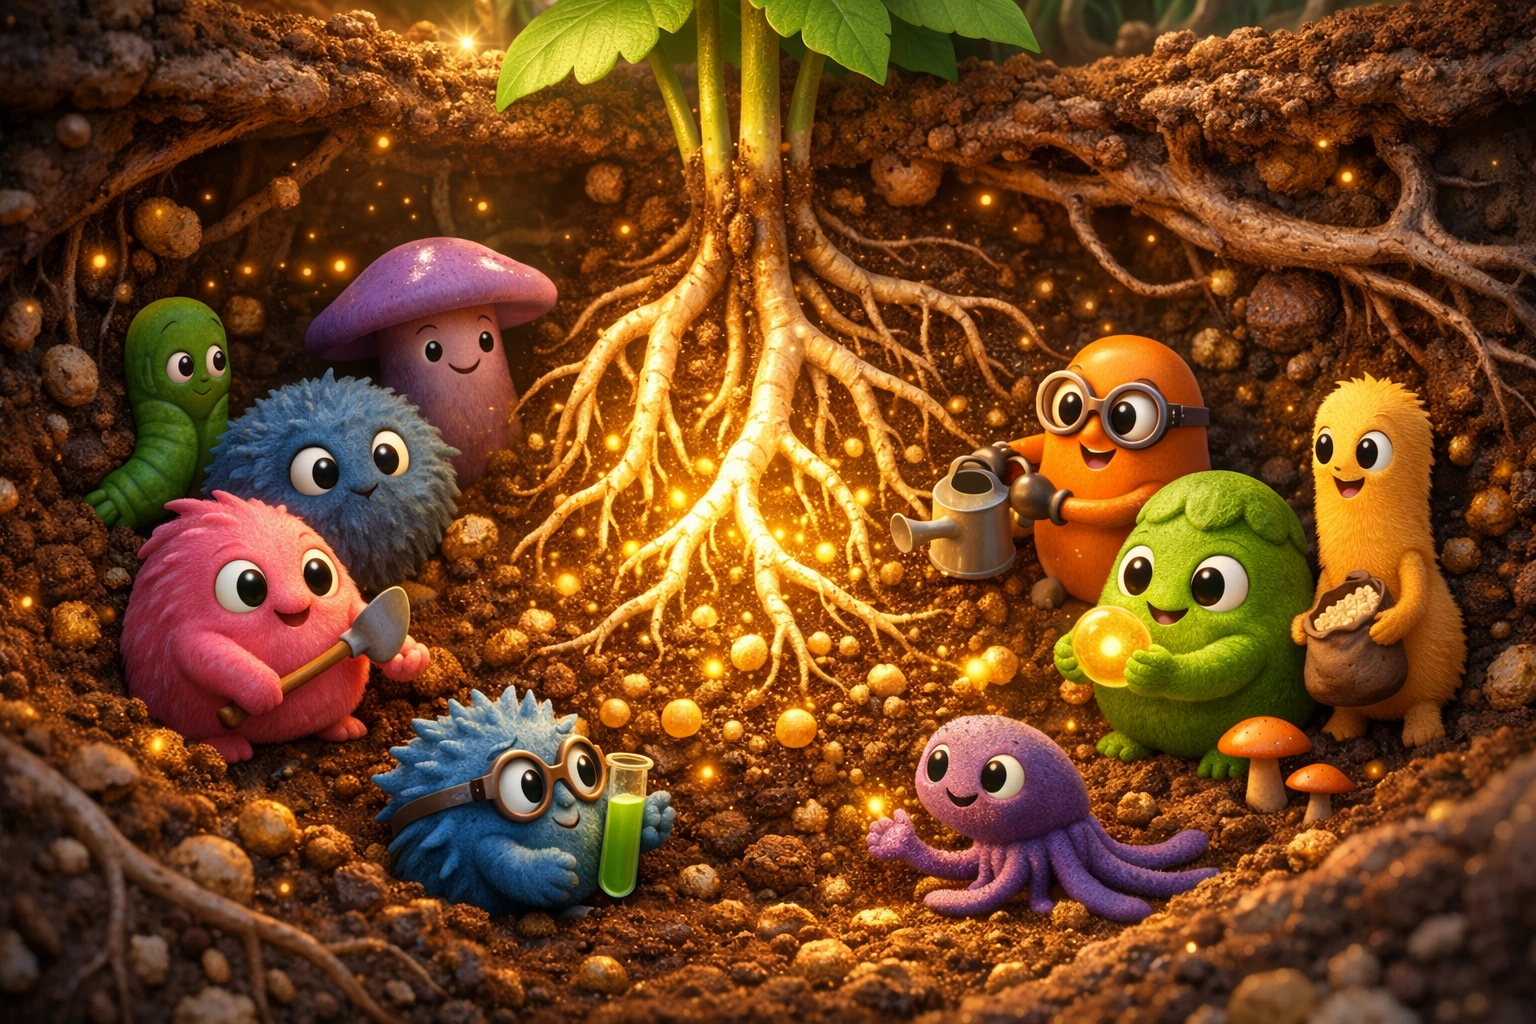
\includegraphics[width=0.85\textwidth]{assets/ch11_lab_manual.png}
    \caption{ภาพรวมการปฏิบัติการจุลชีววิทยาการเกษตรมาตรฐาน แสดงการทำงานภายใต้ตู้ถ่ายเชื้อปลอดเชื้อ (Laminar Airflow Cabinet) การเพาะเลี้ยงเชื้อบนจานอาหารเลี้ยงเชื้อสังเคราะห์ การย้อมสีส่องกล้องจุลทรรศน์ และการวิเคราะห์สารพันธุกรรมด้วยเครื่องเพิ่มปริมาณสารพันธุกรรม PCR}
    \label{fig:ch11_lab_overview}
\end{figure}

\section*{วัตถุประสงค์การเรียนรู้ประจำบท}
เมื่อศึกษาและฝึกปฏิบัติการในบทนี้จบแล้ว นักศึกษาสามารถ:
\begin{enumerate}
    \item ปฏิบัติตนตามระเบียบความปลอดภัยในห้องปฏิบัติการจุลชีววิทยาการเกษตร (Biosafety Level 1 และ 2) ได้อย่างถูกต้อง
    \item ดำเนินการแยก คัดเลือก และทดสอบประสิทธิภาพของ \organism{Rhizobium}, แบคทีเรียละลายฟอสเฟต (PSI), และราปฏิปักษ์ \organism{Trichoderma} (PIRG)
    \item ย้อมสีและประเมินเปอร์เซ็นต์การเข้าอยู่อาศัยของเชื้อราอาร์บัสคูลาร์ไมคอร์ไรซา (AMF) ในรากพืชด้วยวิธี Gridline Intersect Method
    \item ตรวจสอบคุณภาพปุ๋ยชีวภาพทั้งปริมาณเซลล์มีชีวิต (CFU/g) และการตรวจหาเชื้อปนเปื้อนตามมาตรฐาน พ.ร.บ. ปุ๋ย
    \item สกัด DNA จุลินทรีย์จากดิน ตรวจวัดความบริสุทธิ์ด้วยค่า $A_{260}/A_{280}$ และทำปฏิกิริยา PCR สำหรับการตรวจวินิจฉัยเชื้อโรคพืช
\end{enumerate}

\begin{arinteraction}[นวัตกรรมตำราเรียนดิจิทัล: ระบบ AR 3D Interactive ArUco Book]
คู่มือปฏิบัติการในบทนี้ได้รับการออกแบบบูรณาการร่วมกับระบบความจริงเสริม (WebAR) แบบโต้ตอบ 60 FPS ผู้เรียนสามารถใช้สมาร์ตโฟนสแกนรหัส \textbf{ArUco Marker (DICT\_6X6\_250)} ที่ปรากฏคู่กับแต่ละปฏิบัติการ เพื่อเปิดดูแบบจำลอง 3 มิติเสมือนจริง อุปกรณ์แล็บจำลอง และโครงสร้างชีวโมเลกุลสามมิติ (PDB Structures) แบบหมุนสำรวจ $360^\circ$ ได้ทันทีผ่านเบราว์เซอร์โดยไม่ต้องติดตั้งโปรแกรมเพิ่มเติม

\vspace{1mm}
\noindent\textbf{ลิงก์เข้าใช้งานระบบ WebAR:} \url{http://localhost/ar_3d_aruco_book/} หรือใช้ร่วมกับแผ่นพิมพ์การ์ดมาร์กเกอร์ตัดประกอบในไฟล์ \texttt{ar\_markers\_sheet\_A4.pdf}
\end{arinteraction}

\section{ระเบียบความปลอดภัยและเทคนิคปลอดเชื้อ (Aseptic Technique)}

ห้องปฏิบัติการจุลชีววิทยาการเกษตรจัดอยู่ในระดับ \textbf{Biosafety Level 1 (BSL-1)} ถึง \textbf{Biosafety Level 2 (BSL-2)}\index{Biosafety Level (BSL)} นักศึกษาต้องปฏิบัติตามกฎความปลอดภัยอย่างเคร่งครัด:
\begin{enumerate}
    \item \textbf{การเตรียมตัวและการแต่งกาย:} สวมเสื้อกาวน์แขนยาว ถุงมือไนไตรล์ แว่นตานิรภัย และรองเท้าหุ้มส้นตลอดเวลา ห้ามรับประทานอาหาร ดื่มน้ำ หรือสัมผัสใบหน้าระหว่างปฏิบัติการ
    \item \textbf{เทคนิคปลอดเชื้อ (Aseptic Technique):\index{เทคนิคปลอดเชื้อ (Aseptic Technique)}} ทำความสะอาดโต๊ะปฏิบัติการด้วยแอลกอฮอล์ $70\% \text{ (v/v)}$ ก่อนและหลังการทดลอง จุดตะเกียงแอลกอฮอล์เพื่อสร้างรัศมีปลอดเชื้อ $10 - 15\text{ cm}$ หรือปฏิบัติงานในตู้ถ่ายเชื้อปลอดเชื้อ (Laminar Airflow Cabinet) ลนไฟห่วงเพลทเชื้อ (Inoculating loop) จนแดงและปล่อยให้เย็นก่อนสัมผัสโคโลนี
    \item \textbf{การนึ่งฆ่าเชื้อ (Autoclaving):\index{การนึ่งฆ่าเชื้อด้วยไอน้ำ (Autoclaving)}} อาหารเลี้ยงเชื้อ อุปกรณ์แก้ว และของเสียชีวภาพ ต้องผ่านการนึ่งฆ่าเชื้อด้วยไอน้ำอัดความดันที่อุณหภูมิ \textbf{$121^\circ\text{C}$ ความดัน 15 ปอนด์ต่อตารางนิ้ว (psi) เป็นเวลาไม่น้อยกว่า 15--20 นาที}
    \item \textbf{การกำจัดขยะอันตรายชีวภาพ (Biohazard Waste):} ทิ้งจานเพาะเชื้อ ปิเปตทิป และหลอดทดลองที่ปนเปื้อนเชื้อในถังขยะชีวภาพสีแดงเพื่อนำไปผ่านการ Autoclave ก่อนทิ้งสู่ภายนอก
\end{enumerate}

\begin{figure}[ht]
\centering
\resizebox{0.96\textwidth}{!}{
\begin{tikzpicture}[
    level 1/.style={sibling distance=4.5cm, level distance=1.6cm},
    level 2/.style={sibling distance=3.2cm, level distance=1.8cm},
    level 3/.style={sibling distance=2.2cm, level distance=2.0cm},
    root/.style={draw=navyprimary, fill=navyprimary!10, rounded corners=4pt, font=\bfseries\small, text width=3.8cm, align=center, line width=1pt},
    group/.style={draw=forestgreen, fill=forestgreen!10, rounded corners=4pt, font=\bfseries\footnotesize, text width=2.8cm, align=center, line width=0.8pt},
    charact/.style={draw=earthbrown, fill=earthbrown!10, rounded corners=3pt, font=\scriptsize, text width=2.6cm, align=center},
    outcome/.style={draw=navyprimary, fill=amber!20, rounded corners=3pt, font=\bfseries\scriptsize, text width=2.4cm, align=center, line width=0.8pt},
    edge from parent/.style={draw=navyprimary!80, line width=0.8pt, ->, >=Stealth}
]
    \node [root] {การจำแนกจุลินทรีย์การเกษตร\\เบื้องต้นในห้องปฏิบัติการ}
        child {
            node [group] {แบคทีเรียแกรมบวก\\(Gram-Positive)}
            child {
                node [charact] {แท่ง สร้างสปอร์\\Catalase (+)}
                child { node [outcome] {\organism{Bacillus} spp.\\(PGPR / ปุ๋ยชีวภาพ)} }
            }
            child {
                node [charact] {เส้นใยแตกแขนง\\กลิ่นไอดิน (Geosmin)}
                child { node [outcome] {\organism{Streptomyces} spp.\\(ปฏิปักษ์/ย่อยสลาย)} }
            }
        }
        child {
            node [group] {แบคทีเรียแกรมลบ\\(Gram-Negative)}
            child {
                node [charact] {แท่ง สร้างเม็ดสีเรืองแสง\\บนอาหาร King's B}
                child { node [outcome] {\organism{Pseudomonas} spp.\\(ละลายฟอสเฟต/ไซเดอโรฟอร์)} }
            }
            child {
                node [charact] {แยกจากปมรากถั่ว\\อาหาร YEMA+CR ไม่ดูดสี}
                child { node [outcome] {\organism{Rhizobium} spp.\\(ตรึงไนโตรเจนพึ่งพา)} }
            }
        }
        child {
            node [group] {เชื้อราและโอโอไมซีต\\(Fungi / Oomycetes)}
            child {
                node [charact] {โตเร็ว สปอร์สีเขียวเข้ม\\สร้างก้านสปอร์แตกแขนง}
                child { node [outcome] {\organism{Trichoderma} spp.\\(ราปฏิปักษ์ควบคุมโรค)} }
            }
            child {
                node [charact] {เส้นใยไม่มีผนังกั้น\\สปอร์แรนเจียมคล้ายเลมอน}
                child { node [outcome] {\organism{Phytophthora} spp.\\(เชื้อราโรครากเน่า)} }
            }
        };
\end{tikzpicture}
}
\caption{ต้นไม้การตัดสินใจ (Decision Tree) สำหรับการตรวจวินิจฉัยและจำแนกกลุ่มจุลินทรีย์การเกษตรสำคัญในห้องปฏิบัติการ}
\label{fig:microbe_diagnostic_tree}
\end{figure}

\section{ปฏิบัติการที่ 1: การสร้างและศึกษานิเวศวิทยา Winogradsky Column}

\textbf{วัตถุประสงค์:} เพื่อศึกษานิเวศวิทยาจุลินทรีย์ดิน การแบ่งชั้นตามความเข้มข้นของออกซิเจนและซัลไฟด์ และการเติบโตของจุลินทรีย์สังเคราะห์แสง

\begin{labprotocol}[ขั้นตอนการทดลอง Winogradsky Column]
\textbf{วัสดุและอุปกรณ์:} กระบอกตวงพลาสติกหรือขวดแก้วใสทรงสูง (ขนาด $500 - 1,000\text{ mL}$), โคลนจากท้องร่องสวนหรือก้นหนองน้ำ, กระดาษกรองสับละเอียด $5\text{ g}$ (แหล่งคาร์บอนเซลลูโลส), แคลเซียมซัลเฟต ($CaSO_4$) $5\text{ g}$, แคลเซียมคาร์บอเนต ($CaCO_3$) $5\text{ g}$, แรปพลาสติกใส, โคมไฟส่องสว่างหลอดไส้ 40--60 วัตต์

\textbf{ขั้นตอนการทำปฏิบัติการ:}
\begin{enumerate}
    \item นำดินโคลนมาผสมกับ $CaSO_4, CaCO_3$ และเศษกระดาษกรองสับให้เข้ากันเป็นเนื้อเดียว
    \item บรรจุส่วนผสมดินโคลนลงในกระบอกแก้วให้สูงประมาณ $1/3$ เคาะไล่ฟองอากาศให้แน่น
    \item ตักดินโคลนที่ไม่ผสมสารเคมีเติมลงไปต่อจนสูงถึง $2/3$ ของกระบอก
    \item เติมน้ำจากแหล่งน้ำธรรมชาติลงไปจนเหลือช่องว่างอากาศด้านบนประมาณ $2 - 3\text{ cm}$
    \item ปิดปากกระบอกด้วยแรปพลาสติกใสและรัดหนังยางให้แน่นเพื่อป้องกันน้ำระเหย
    \item วางกระบอกตวงไว้ใกล้หน้าต่างหรือส่องด้วยโคมไฟห่างประมาณ 20 ซม. บ่มไว้เป็นเวลา 4--8 สัปดาห์
    \item สังเกตการแบ่งชั้นสีของจุลินทรีย์: ชั้นล่างสุดสีดำ (\organism{Desulfovibrio}), ชั้นสีเขียวเข้ม (Green sulfur bacteria: \organism{Chlorobium}), ชั้นสีแดงอมม่วง (Purple sulfur bacteria: \organism{Chromatium}), และชั้นผิวน้ำสีเขียวสว่าง (Algae และ Cyanobacteria)
\end{enumerate}
\end{labprotocol}

\begin{arinteraction}[AR 3D Interactive Simulation: Winogradsky Eco-Column (ArUco ID: 0)]
\begin{minipage}[c]{0.26\textwidth}
    \centering
    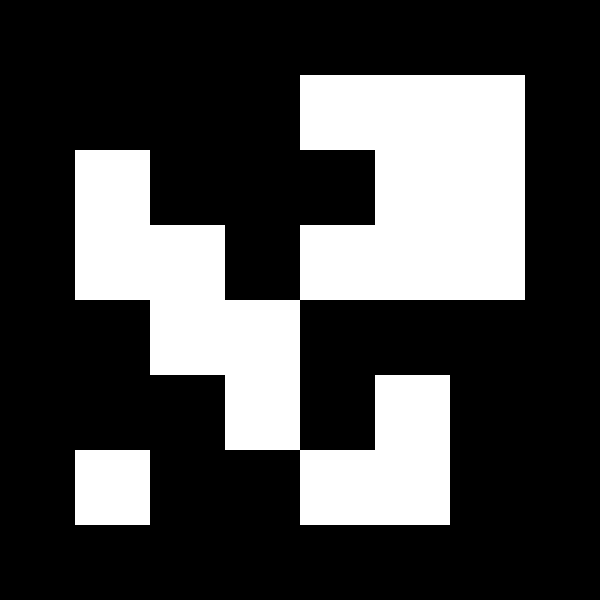
\includegraphics[width=\linewidth]{assets/aruco/aruco_id_0.png}
\end{minipage}\hfill
\begin{minipage}[c]{0.70\textwidth}
    \small
    \textbf{ส่องด้วยสมาร์ตโฟนผ่าน WebAR เพื่อดูแบบจำลอง 3 มิติเสมือนจริง}\\
    \textbf{แบบจำลอง 3D:} Winogradsky Eco-Column หลอดทดลอง 4 ชั้นนิเวศจุลินทรีย์ดิน\\
    \textbf{ฟังก์ชันเชิงโต้ตอบ:} หมุนสำรวจการแบ่งชั้นจุลินทรีย์ (\organism{Desulfovibrio}, \organism{Chlorobium}, \organism{Chromatium}, \organism{Cyanobacteria}) และการไล่ระดับความเข้มข้นสัมพัทธ์ของก๊าซ $O_2$ และ $H_2S$ แบบเรียลไทม์ 60 FPS
\end{minipage}
\end{arinteraction}

\section{ปฏิบัติการที่ 2: การแยกและทดสอบประสิทธิภาพ Rhizobium จากปมรากถั่ว}

\textbf{วัตถุประสงค์:} เพื่อแยกเชื้อบริสุทธิ์ของ \organism{Rhizobium}\index{Rhizobium@\textit{Rhizobium}} และประเมินความมีชีวิตของโปรตีนเลกเฮโมโกลบินในปมราก

\begin{labprotocol}[ขั้นตอนการแยกเชื้อ Rhizobium]
\textbf{วัสดุและอุปกรณ์:} ปมรากถั่วสดที่มีสีชมพูเรื่อด้านใน, เอทานอล 70\%, สารละลายโซเดียมไฮโปคลอไรต์ 1\%, น้ำกลั่นนึ่งฆ่าเชื้อ, อาหาร Yeast Extract Mannitol Agar ผสม Congo Red (YEMA-CR)\index{อาหารเลี้ยงเชื้อ YEMA (Yeast Extract Mannitol Agar)}, แท่งแก้วบดปลอดเชื้อ

\textbf{ขั้นตอนการทำปฏิบัติการ:}
\begin{enumerate}
    \item เลือกปมรากที่สมบูรณ์ ผ่าครึ่งเพื่อยืนยันสีชมพูของเลกเฮโมโกลบิน (Active nitrogen fixation)
    \item จุ่มปมรากในเอทานอล 70\% นาน 10 วินาที จากนั้นย้ายลงในสารละลายไฮโปคลอไรต์ 1\% นาน 3 นาที เพื่อฟอกฆ่าเชื้อที่ผิว (Surface sterilization)
    \item ล้างน้ำกลั่นนึ่งฆ่าเชื้อ 5 ครั้งเพื่อกำจัดสารฟอกขาวตกค้าง
    \item ใส่ปมรากลงในหลอดทดลอง เติมน้ำกลั่นปลอดเชื้อ $0.2\text{ mL}$ แล้วบดด้วยแท่งแก้วจนละเอียด
    \item แตะสารแขวนลอยนำมาเกลี่ยแบบ Streak plate บนอาหาร YEMA-CR บ่มที่ $28^\circ\text{C}$ นาน 3--5 วัน
    \item ตรวจดูลักษณะโคโลนี: \organism{Rhizobium} จะมีลักษณะกลมนูน เมือกเหนียวขุ่น สีขาวหรือชมพูอ่อนมาก โดย \textbf{ไม่ดูดซับสีย้อมคองโกเรด} เข้าสู่เซลล์ (ต่างจากแบคทีเรียปนเปื้อนที่ติดสีแดงเข้ม)
\end{enumerate}
\end{labprotocol}

\begin{arinteraction}[AR 3D Interactive Simulation: Rhizobium \& Leghemoglobin 1GDJ (ArUco ID: 1)]
\begin{minipage}[c]{0.26\textwidth}
    \centering
    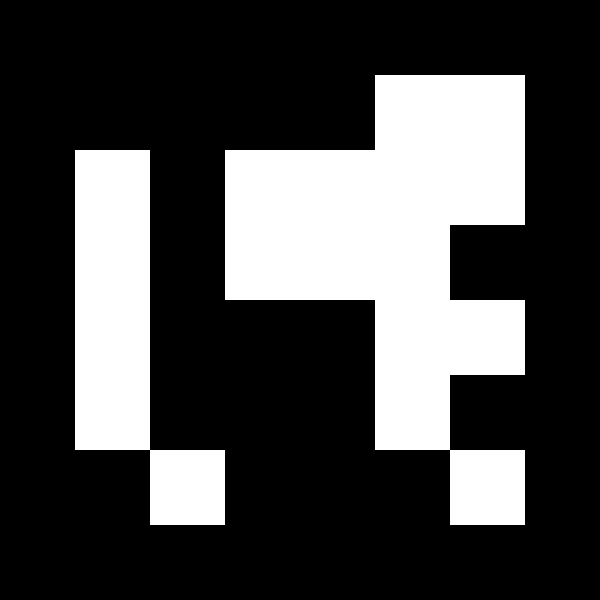
\includegraphics[width=\linewidth]{assets/aruco/aruco_id_1.png}
\end{minipage}\hfill
\begin{minipage}[c]{0.70\textwidth}
    \small
    \textbf{ส่องด้วยสมาร์ตโฟนผ่าน WebAR เพื่อดูแบบจำลอง 3 มิติเสมือนจริง}\\
    \textbf{แบบจำลอง 3D:} โครงสร้างปมรากถั่วผ่าซีก และโครงสร้างโมเลกุล 3D โปรตีนเลกเฮโมโกลบิน (\textit{Leghemoglobin}, PDB ID: \texttt{1GDJ})\\
    \textbf{ฟังก์ชันเชิงโต้ตอบ:} สำรวจโครงข่ายฮีมพ็อกเก็ต (Heme pocket) ดักจับโมเลกุลออกซิเจน เพื่อรักษาสภาวะไม่ใช้ออกซิเจนแก่เอนไซม์ไนโตรจีเนสในแบคทีรอยด์
\end{minipage}
\end{arinteraction}

\section{ปฏิบัติการที่ 3: การคัดเลือกจุลินทรีย์ละลายฟอสเฟต (PSI)}

\textbf{วัตถุประสงค์:} เพื่อคัดแยกจุลินทรีย์ที่มีศักยภาพละลายฟอสเฟตและคำนวณดัชนี Phosphate Solubilization Index (PSI)\index{Phosphate Solubilization Index (PSI)}

\begin{labprotocol}[ขั้นตอนการวัดค่าดัชนี PSI บนอาหาร Pikovskaya]
\textbf{วัสดุและอุปกรณ์:} อาหารแข็ง Pikovskaya's Agar\index{อาหารเลี้ยงเชื้อ Pikovskaya} (มีตะกอนแคลเซียมฟอสเฟต $Ca_3(PO_4)_2$ สีขาวขุ่น), หัวเชื้อจุลินทรีย์ดินตัวอย่าง, เวอร์เนียคาลิปเปอร์

\textbf{ขั้นตอนการทำปฏิบัติการ:}
\begin{enumerate}
    \item จุดหัวเชื้อ (Spot inoculation) ปริมาตร $10\mu\text{L}$ ลงบนกึ่งกลางจานอาหาร Pikovskaya จำนวน 3 ซ้ำ
    \item บ่มที่อุณหภูมิ $30^\circ\text{C}$ เป็นเวลา 5 วัน (แบคทีเรีย) หรือ 7 วัน (เชื้อรา)
    \item วัดเส้นผ่านศูนย์กลางของโคโลนี ($d_c$) และเส้นผ่านศูนย์กลางของวงใส (Clear zone diameter: $d_z$) ด้วยเวอร์เนียคาลิปเปอร์
    \item คำนวณค่าดัชนีการละลายฟอสเฟต:
    \begin{equation}
    \text{PSI} = \frac{d_z}{d_c}
    \end{equation}
\end{enumerate}
เกณฑ์การประเมิน: ค่า $\text{PSI} \ge 2.0$ จัดเป็นจุลินทรีย์ที่มีประสิทธิภาพสูงมากในการปลดปล่อยฟอสฟอรัส
\end{labprotocol}

\begin{arinteraction}[AR 3D Interactive Simulation: Phosphate Solubilizer PSI Assay (ArUco ID: 2)]
\begin{minipage}[c]{0.26\textwidth}
    \centering
    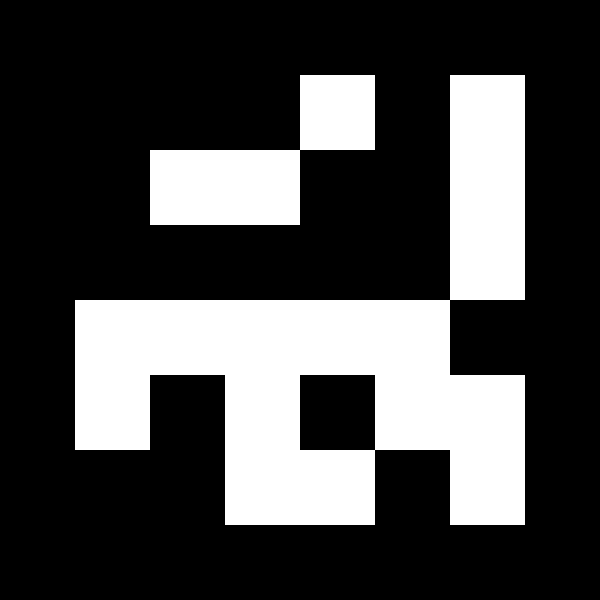
\includegraphics[width=\linewidth]{assets/aruco/aruco_id_2.png}
\end{minipage}\hfill
\begin{minipage}[c]{0.70\textwidth}
    \small
    \textbf{ส่องด้วยสมาร์ตโฟนผ่าน WebAR เพื่อดูแบบจำลอง 3 มิติเสมือนจริง}\\
    \textbf{แบบจำลอง 3D:} จานเพาะเชื้อ Pikovskaya Agar แสดงโคโลนีและวงใสละลายหินฟอสเฟต (Clear Zone) พร้อมเวอร์เนียคาลิปเปอร์จำลอง\\
    \textbf{ฟังก์ชันเชิงโต้ตอบ:} ปรับเลื่อนแถบเวอร์เนียวัดขนาดเส้นผ่านศูนย์กลาง $d_z$ และ $d_c$ พร้อมระบบคำนวณและประเมินค่าดัชนี $\text{PSI} = d_z / d_c$ โดยอัตโนมัติ
\end{minipage}
\end{arinteraction}

\section{ปฏิบัติการที่ 4: การทดสอบกิจกรรมปฏิปักษ์ของ Trichoderma (PIRG)}

\textbf{วัตถุประสงค์:} เพื่อประเมินความสามารถในการยับยั้งเชื้อราก่อโรคพืชของ \organism{Trichoderma harzianum} ด้วยเทคนิค Dual Culture\index{Dual Culture Assay}

\begin{labprotocol}[ขั้นตอนการทดสอบ Dual Culture Confrontation Assay]
\textbf{วัสดุและอุปกรณ์:} อาหาร Potato Dextrose Agar (PDA), จานเลี้ยงเชื้อ \organism{Trichoderma harzianum} อายุ 5 วัน, จานเลี้ยงเชื้อราก่อโรค (เช่น \organism{Fusarium oxysporum} หรือ \organism{Colletotrichum} sp.), Cork borer ขนาดเส้นผ่านศูนย์กลาง $5\text{ mm}$

\textbf{ขั้นตอนการทำปฏิบัติการ:}
\begin{enumerate}
    \item ใช้ Cork borer เจาะชิ้นวุ้นขอบโคโลนีราก่อโรค วางลงบนจานอาหาร PDA ห่างจากขอบจาน $1.5\text{ cm}$
    \item เจาะชิ้นวุ้นราปฏิปักษ์ \organism{Trichoderma} วางตรงข้ามกันห่างจากขอบอีกด้าน $1.5\text{ cm}$ (ระยะห่างระหว่างชิ้นวุ้นทั้งสองประมาณ $5.0\text{ cm}$)
    \item ทำจานควบคุม (Control plate) โดยวางชิ้นวุ้นราก่อโรคเพียงอย่างเดียว
    \item บ่มที่อุณหภูมิห้อง ($25-28^\circ\text{C}$) ตรวจวัดรัศมีการเจริญของเชื้อราก่อโรคเข้าหาเชื้อปฏิปักษ์ ($R_2$) และวัดรัศมีเชื้อราก่อโรคในจานควบคุม ($R_1$) เมื่อจานควบคุมเจริญเกือบเต็มจาน (ประมาณวันที่ 5--7)
    \item คำนวณเปอร์เซ็นต์การยับยั้งการเจริญของรัศมีเส้นใย:
    \begin{equation}
    \text{PIRG (\%)} = \frac{R_1 - R_2}{R_1} \times 100
    \end{equation}
\end{enumerate}
\end{labprotocol}

\begin{arinteraction}[AR 3D Interactive Simulation: Trichoderma Confrontation \& Chitinase 1CTN (ArUco ID: 3)]
\begin{minipage}[c]{0.26\textwidth}
    \centering
    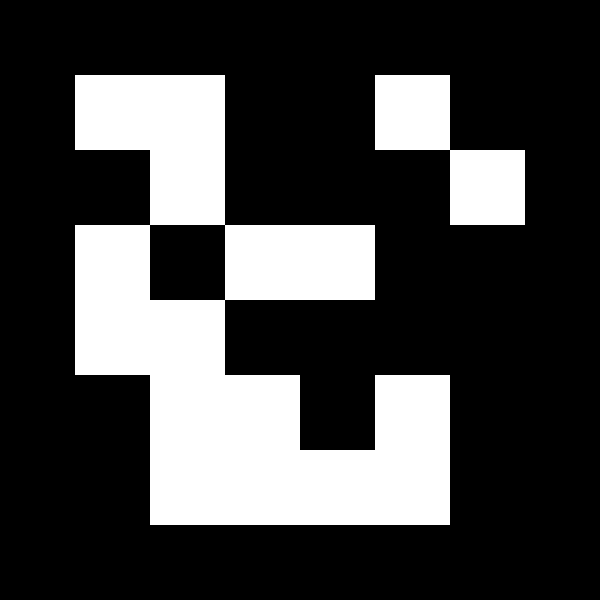
\includegraphics[width=\linewidth]{assets/aruco/aruco_id_3.png}
\end{minipage}\hfill
\begin{minipage}[c]{0.70\textwidth}
    \small
    \textbf{ส่องด้วยสมาร์ตโฟนผ่าน WebAR เพื่อดูแบบจำลอง 3 มิติเสมือนจริง}\\
    \textbf{แบบจำลอง 3D:} จานประจันหน้า Dual Culture (\organism{Trichoderma} ปะทะ \organism{Fusarium}) และโมเลกุลเอนไซม์ไคติเนส (\textit{Chitinase}, PDB ID: \texttt{1CTN})\\
    \textbf{ฟังก์ชันเชิงโต้ตอบ:} จำลองกลไก Mycoparasitism การแทงเส้นใยพันรัด ปลดปล่อยเอนไซม์ย่อยสลายผนังเซลล์ราโรคพืช และคำนวณค่า PIRG (\%)
\end{minipage}
\end{arinteraction}

\section{ปฏิบัติการที่ 5: การย้อมสีและตรวจหาเชื้อราไมคอร์ไรซาในรากพืช}

\textbf{วัตถุประสงค์:} เพื่อเตรียมสไลด์รากพืช ย้อมสีโครงสร้างอาร์บัสคูลและเวสิเคิลของ AMF และประเมินเปอร์เซ็นต์การเข้าอยู่อาศัยในราก

\begin{labprotocol}[การย้อมสีรากด้วยวิธี Trypan Blue และวิธี Gridline Intersect]
\textbf{วัสดุและอุปกรณ์:} รากฝอยพืชสด (ข้าวโพดหรือหญ้า), สารละลายโพแทสเซียมไฮดรอกไซด์ (KOH) 10\%, กรดไฮโดรคลอริก (HCl) 1\%, สีย้อม Trypan Blue 0.05\% ในแลกโตกลีเซอรอล\index{การย้อมสีย้อม Trypan Blue}, จานเพาะเชื้อกริดตาราง (Gridline dish), กล้องจุลทรรศน์สเตอริโอและกล้องเลนส์ประกอบ

\textbf{ขั้นตอนการทำปฏิบัติการ:}
\begin{enumerate}
    \item ล้างรากพืชให้สะอาด ตัดเป็นท่อนยาวประมาณ $1\text{ cm}$
    \item แช่รากในสารละลาย KOH 10\% ในอ่างน้ำร้อน ($90^\circ\text{C}$) นาน 30--45 นาที เพื่อฟอกล้างไซโตพลาสซึมของเซลล์พืช (Root Clearing)
    \item ล้างด้วยน้ำสะอาด แล้วแช่ในสารละลาย HCl 1\% นาน 5 นาที เพื่อปรับสภาพความเป็นกรด
    \item ย้ายรากลงแช่ในสีย้อม Trypan Blue 0.05\% ในอ่างน้ำร้อน ($90^\circ\text{C}$) นาน 15 นาที
    \item ล้างสีส่วนเกินออกด้วยสารละลายแลกโตกลีเซอรอลบริสุทธิ์
    \item นำชิ้นราก 50--100 ชิ้นมาเรียงบนจานแก้วที่มีเส้นกริดตารางขนาด $0.5 \times 0.5\text{ cm}$ ส่องตรวจจุดตัดระหว่างเส้นกริดกับชิ้นราก (Gridline Intersect Method)\index{Gridline Intersect Method}
    \item ตรวจนับจุดตัดที่มีโครงสร้าง AMF (Arbuscules, Vesicles, Hyphae) และจุดตัดทั้งหมด
    \begin{equation}
    \% \text{ AMF Colonization} = \frac{\text{จำนวนจุดตัดที่พบโครงสร้าง AMF}}{\text{จำนวนจุดตัดของรากทั้งหมด}} \times 100
    \end{equation}
\end{enumerate}
\end{labprotocol}

\begin{arinteraction}[AR 3D Interactive Simulation: AMF Root Colonization \& Gridline (ArUco ID: 4)]
\begin{minipage}[c]{0.26\textwidth}
    \centering
    
\includegraphics[width=\linewidth]{assets/aruco/aruco_id_4.png}
\end{minipage}\hfill
\begin{minipage}[c]{0.70\textwidth}
    \small
    \textbf{ส่องด้วยสมาร์ตโฟนผ่าน WebAR เพื่อดูแบบจำลอง 3 มิติเสมือนจริง}\\
    \textbf{แบบจำลอง 3D:} รากพืชย้อมสี Trypan Blue โครงสร้าง Arbuscule, Vesicle และจานแก้วกริดตาราง\\
    \textbf{ฟังก์ชันเชิงโต้ตอบ:} จำลองการเลื่อนส่องกล้องตรวจจุดตัด Gridline Intersect Method และคำนวณ \% AMF Colonization โดยอัตโนมัติ
\end{minipage}
\end{arinteraction}

\section{ปฏิบัติการที่ 6: การวิเคราะห์คุณภาพปุ๋ยชีวภาพและการตรวจหาเชื้อปนเปื้อน}

\textbf{วัตถุประสงค์:} เพื่อตรวจนับจำนวนเซลล์มีชีวิตของแบคทีเรียปุ๋ยชีวภาพด้วยเทคนิค Serial Dilution Pour Plate และตรวจคัดกรองเชื้อปนเปื้อนตามมาตรฐานกรมวิชาการเกษตร

\begin{labprotocol}[การตรวจสอบคุณภาพปุ๋ยชีวภาพตามกฎหมาย]
\textbf{วัสดุและอุปกรณ์:} ตัวอย่างปุ๋ยชีวภาพ, สารละลายน้ำเกลือปราศจากเชื้อ 0.85\% NaCl, ปิเปตอัตโนมัติ, อาหารจำเพาะ (YEMA สำหรับ Rhizobium, NA สำหรับนับเชื้อรวม, MacConkey Agar สำหรับตรวจเชื้อกลุ่มโคลิฟอร์ม)\index{อาหาร MacConkey Agar}, ตู้อบเพาะเชื้อ

\textbf{ขั้นตอนการทำปฏิบัติการ:}
\begin{enumerate}
    \item ชั่งตัวอย่างปุ๋ยชีวภาพ $10.0\text{ g}$ ใส่ลงในขวดน้ำเกลือปลอดเชื้อ $90.0\text{ mL}$ เขย่าที่ $180\text{ rpm}$ นาน 30 นาที (ระดับเจือจาง $10^{-1}$)
    \item ดูดสารละลาย $1.0\text{ mL}$ ถ่ายลงในหลอดน้ำเกลือ $9.0\text{ mL}$ ทำการเจือจางแบบสิบเท่าต่อเนื่อง\index{การเจือจางแบบลำดับส่วน (Serial Dilution)}จนถึงระดับ $10^{-8}$
    \item ดูดสารละลายจากระดับเจือจาง $10^{-5}, 10^{-6}, 10^{-7}$ ปริมาตรละ $0.1\text{ mL}$ ลงบนจานอาหารจำเพาะ เกลี่ยด้วยแท่งแก้วสามเหลี่ยม (Spread plate) จานละ 3 ซ้ำ
    \item ดูดสารละลายระดับเจือจาง $10^{-1}$ และ $10^{-2}$ ปริมาตร $0.1\text{ mL}$ เกลี่ยลงบนอาหาร MacConkey Agar เพื่อตรวจหาแบคทีเรียกลุ่มปนเปื้อน \organism{E. coli}
    \item บ่มที่ $30^\circ\text{C}$ นาน 48 ชั่วโมง ตรวจนับจานอาหารที่มีโคโลนีระหว่าง 30--300 โคโลนี คำนวณค่า CFU/g\index{หน่วยนับโคโลนี (CFU)}
    \item ตรวจสอบว่ามีโคโลนีสีชมพูเข้มบน MacConkey Agar หรือไม่ (หากพบแสดงว่าไม่ผ่านเกณฑ์มาตรฐานการปนเปื้อน)
\end{enumerate}
\end{labprotocol}

\begin{arinteraction}[AR 3D Interactive Simulation: Biofertilizer QC \& Dilution (ArUco ID: 5)]
\begin{minipage}[c]{0.26\textwidth}
    \centering
    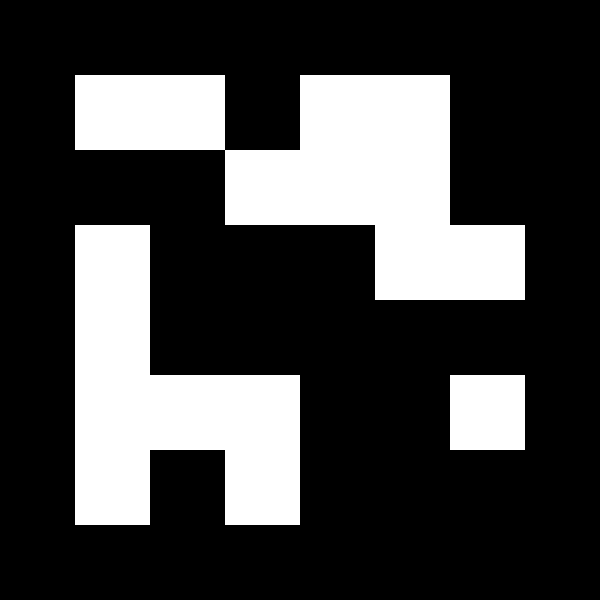
\includegraphics[width=\linewidth]{assets/aruco/aruco_id_5.png}
\end{minipage}\hfill
\begin{minipage}[c]{0.70\textwidth}
    \small
    \textbf{ส่องด้วยสมาร์ตโฟนผ่าน WebAR เพื่อดูแบบจำลอง 3 มิติเสมือนจริง}\\
    \textbf{แบบจำลอง 3D:} แร็คหลอดทดลองการเจือจางสิบเท่า ($10^{-1}$ ถึง $10^{-6}$) และจานเพาะเชื้อ MacConkey Agar\\
    \textbf{ฟังก์ชันเชิงโต้ตอบ:} จำลองการตรวจนับโคโลนี CFU/g และการตรวจสอบเชื้อปนเปื้อนกลุ่มโคลิฟอร์มตามมาตรฐาน พ.ร.บ. ปุ๋ย
\end{minipage}
\end{arinteraction}

\section{ปฏิบัติการที่ 7: การสกัด Soil DNA และการตรวจสอบคุณภาพ}

\textbf{วัตถุประสงค์:} เพื่อสกัดสารพันธุกรรม DNA ของไมโครไบโอมดินด้วยเทคนิค Bead-Beating และประเมินความบริสุทธิ์ของ DNA\index{การสกัด DNA จุลินทรีย์ดิน (Soil DNA Extraction)}

\begin{labprotocol}[ขั้นตอนการสกัด Soil Metagenomic DNA]
\textbf{วัสดุและอุปกรณ์:} ตัวอย่างดินไรโซสเฟียร์ $0.25\text{ g}$, ชุดสกัดดิน DNeasy PowerSoil Pro Kit (หรือวิธี Bead-beating CTAB/Phenol-chloroform), เครื่องโฮโมจีไนเซอร์ความเร็วสูง (Bead beater), เครื่องหมุนเหวี่ยงความเย็นสูง, เครื่องสเปกโทรโฟโตมิเตอร์ไมโครวอลุม (Nanodrop)\index{เครื่องสเปกโทรโฟโตมิเตอร์ Nanodrop}, ชุดเจลอิเล็กโทรโฟรซิส

\textbf{ขั้นตอนการทำปฏิบัติการ:}
\begin{enumerate}
    \item ชั่งดิน $0.25\text{ g}$ ใส่ลงในหลอดบรรจุลูกปัดซิลิกา (PowerBead Tube) เติม Lysis Buffer เพื่อช่วยทำลายผนังเซลล์
    \item นำเข้าเครื่อง Bead Beater ปั่นสั่นสะเทือนที่ความเร็ว $6.0\text{ m/s}$ เป็นเวลา 45 วินาที เพื่อทำลายผนังเซลล์แบคทีเรีย แกรมบวก แอคติโนมัยซีส และสปอร์รา
    \item หมุนเหวี่ยงตกตะกอนเศษดินและโปรตีน ดูดสารละลายใสส่วนบนถ่ายลงในหลอดใหม่ เติม Inhibitor Removal Solution เพื่อตกตะกอนกรดฮิวมิก (Humic acids ซึ่งเป็นสารยับยั้งปฏิกิริยา PCR)
    \item ผ่านสารละลายผ่านคอลัมน์ซิลิกา (Silica Spin Column) หมุนเหวี่ยงเพื่อให้ DNA ยึดเกาะกับเยื่อซิลิกา
    \item ล้างคอลัมน์ด้วย Wash Buffer ที่มีเอทานอล 2 ครั้ง หมุนเหวี่ยงเพื่อไล่เอทานอลให้แห้งสนิท
    \item ละลาย DNA ออกจากคอลัมน์ด้วยน้ำปราศจากเอนไซม์นิวคลีเอส (Nuclease-free water) $50\mu\text{L}$
    \item วัดค่าการดูดกลืนแสงที่ความยาวคลื่น $260\text{ nm}$ ($A_{260}$) และ $280\text{ nm}$ ($A_{280}$) ด้วยเครื่อง Nanodrop:
    \begin{itemize}
        \item ความเข้มข้นของ DNA ($\text{ng/}\mu\text{L}$) $= A_{260} \times 50 \times \text{Dilution factor}$
        \item อัตราส่วนความบริสุทธิ์: ค่า $A_{260}/A_{280}$ ที่เหมาะสมควรอยู่ในช่วง \textbf{$1.8 - 2.0$} (หากต่ำกว่า 1.8 แสดงว่ามีโปรตีนหรือกรดฮิวมิกปนเปื้อน)
    \end{itemize}
    \item ตรวจสอบขนาดความสมบูรณ์ของสาย DNA ด้วย Agarose Gel Electrophoresis 1\%\index{เจลอิเล็กโทรโฟริซิส (Agarose Gel Electrophoresis)}
\end{enumerate}
\end{labprotocol}

\begin{arinteraction}[AR 3D Interactive Simulation: Soil DNA Extraction \& B-DNA 1BNA (ArUco ID: 6)]
\begin{minipage}[c]{0.26\textwidth}
    \centering
    
\includegraphics[width=\linewidth]{assets/aruco/aruco_id_6.png}
\end{minipage}\hfill
\begin{minipage}[c]{0.70\textwidth}
    \small
    \textbf{ส่องด้วยสมาร์ตโฟนผ่าน WebAR เพื่อดูแบบจำลอง 3 มิติเสมือนจริง}\\
    \textbf{แบบจำลอง 3D:} หลอด Bead-Beater Lysis, Spin Column, เกลียวคู่ Double-Helix B-DNA (PDB ID: \texttt{1BNA}) และเครื่อง Nanodrop\\
    \textbf{ฟังก์ชันเชิงโต้ตอบ:} หมุนดูโครงสร้างโมเลกุลเกลียวคู่ และกราฟสเปกตรัมดูดกลืนแสง $A_{260}/A_{280}$ ประเมินความบริสุทธิ์ของ DNA
\end{minipage}
\end{arinteraction}

\section{ปฏิบัติการที่ 8: การตรวจวินิจฉัยโรคพืชด้วย PCR และการประเมินภาพด้วย OpenCV}

\textbf{วัตถุประสงค์:} เพื่อเพิ่มปริมาณยีนจำเพาะของเชื้อก่อโรคพืชด้วยปฏิกิริยา Polymerase Chain Reaction (PCR)\index{ปฏิกิริยาลูกโซ่พอลิเมอเรส (PCR)} และประเมินร้อยละพื้นที่แผลบนใบพืชด้วยสคริปต์คอมพิวเตอร์วิทัศน์\index{OpenCV!การคำนวณพื้นที่แผลโรคพืช}

\begin{labprotocol}[ขั้นตอนการทำปฏิกิริยา PCR และการประมวลผลภาพ]
\textbf{ส่วนที่ 1: การทำปฏิกิริยา PCR ตรวจเชื้อ Phytophthora palmivora}
\begin{enumerate}
    \item ผสมสารละลายปฏิกิริยา PCR Master Mix ปริมาตรรวม $25\mu\text{L}$ ต่อหลอด:
    \begin{itemize}
        \item $2\times$ Taq MasterMix (dNTPs, Taq polymerase, Buffer): $12.5\mu\text{L}$
        \item Forward Primer (10 $\mu$M): $1.0\mu\text{L}$
        \item Reverse Primer (10 $\mu$M): $1.0\mu\text{L}$
        \item DNA แม่แบบ (สกัดจากเนื้อเยื่อใบพืชที่เป็นโรค): $2.0\mu\text{L}$ ($20-50\text{ ng}$)
        \item Nuclease-free water: $8.5\mu\text{L}$
    \end{itemize}
    \item โปรแกรมเครื่อง Thermal Cycler:
    \begin{itemize}
        \item Initial Denaturation: $95^\circ\text{C}$ นาน 5 นาที
        \item 35 รอบของ: $95^\circ\text{C}$ (30 วินาที) $\rightarrow 58^\circ\text{C}$ (30 วินาที) $\rightarrow 72^\circ\text{C}$ (45 วินาที)
        \item Final Extension: $72^\circ\text{C}$ นาน 5 นาที
    \end{itemize}
    \item นำผลิตภัณฑ์ PCR ตรวจสอบบนเจลอะกาโรส 1.5\% เทียบกับดีเอ็นเอมาตรฐาน (DNA Ladder 100 bp) สังเกตแถบยีนขนาดจำเพาะ
\end{enumerate}

\textbf{ส่วนที่ 2: การประเมินพื้นที่แผลโรคพืชด้วย Python OpenCV}
\begin{enumerate}
    \item ถ่ายภาพใบพืชที่เป็นโรคบนพื้นหลังสีขาวภายใต้แสงสม่ำเสมอ
    \item รันสคริปต์ Python ในภาคผนวก ข เพื่อแปลงภาพเป็นปริภูมิสี HSV ตัดแยกพิกเซลใบและพิกเซลแผลสะเก็ด
    \item บันทึกค่าร้อยละพื้นที่ความรุนแรงของโรค (DSI) เพื่อนำไปเปรียบเทียบกับผลการตรวจทางอณูชีววิทยา
\end{enumerate}
\end{labprotocol}

\begin{arinteraction}[AR 3D Interactive Simulation: PCR Thermal Cycler \& Vision AI (ArUco ID: 7)]
\begin{minipage}[c]{0.26\textwidth}
    \centering
    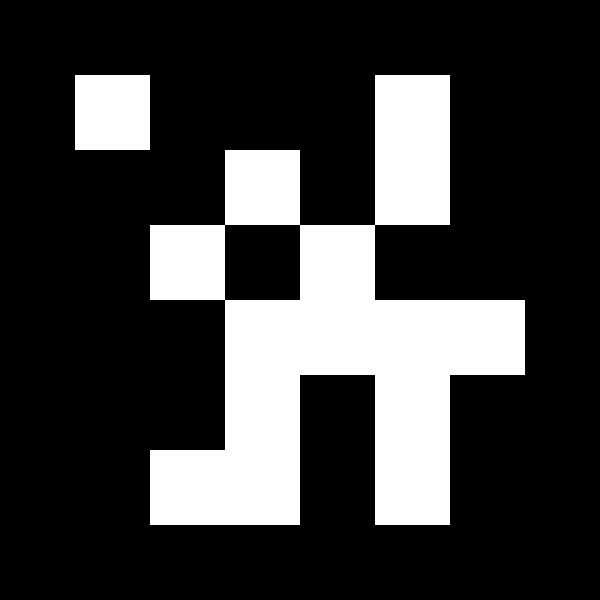
\includegraphics[width=\linewidth]{assets/aruco/aruco_id_7.png}
\end{minipage}\hfill
\begin{minipage}[c]{0.70\textwidth}
    \small
    \textbf{ส่องด้วยสมาร์ตโฟนผ่าน WebAR เพื่อดูแบบจำลอง 3 มิติเสมือนจริง}\\
    \textbf{แบบจำลอง 3D:} เครื่อง Mini PCR Thermal Cycler, ถาดเจลอะกาโรสเรืองแสง UV, เอนไซม์ Taq Polymerase (PDB ID: \texttt{1TAU}) และ OpenCV Bounding Box\\
    \textbf{ฟังก์ชันเชิงโต้ตอบ:} แสดงวงรอบอุณหภูมิ 3 ระดับ การตรวจสอบแถบขนาดดีเอ็นเอ และการตัดตรวจพื้นที่แผลสะเก็ดโรคพืช (DSI \%)
\end{minipage}
\end{arinteraction}

\begin{worked}[ตัวอย่างที่ 11.1 การคำนวณความเข้มข้นและความบริสุทธิ์ของ Soil Metagenomic DNA]
นักศึกษาใช้เครื่อง Nanodrop ตรวจวัดสารละลาย DNA ที่สกัดได้จากดินสวนทุเรียน ได้ค่าการดูดกลืนแสงดังนี้:
$$A_{260} = 0.840 \quad , \quad A_{280} = 0.450 \quad , \quad A_{230} = 0.380$$
จงคำนวณหาความเข้มข้นของ DNA ($\text{ng/}\mu\text{L}$), อัตราส่วนความบริสุทธิ์ $A_{260}/A_{280}$ และ $A_{260}/A_{230}$ พร้อมวิเคราะห์ว่าตัวอย่างนี้สามารถนำไปทำ PCR ได้ทันทีหรือไม่

\textbf{วิธีทำ:}
1. คำนวณความเข้มข้นของ DNA ($1\text{ หน่วย } A_{260} = 50\text{ ng/}\mu\text{L}$ ของ dsDNA):
$$\text{DNA Concentration} = A_{260} \times 50 = 0.840 \times 50 = \mathbf{42.0\text{ ng/}\mu\text{L}}$$

2. คำนวณอัตราส่วนความบริสุทธิ์ $A_{260}/A_{280}$:
$$\frac{A_{260}}{A_{280}} = \frac{0.840}{0.450} \approx \mathbf{1.867}$$

3. คำนวณอัตราส่วนความบริสุทธิ์ $A_{260}/A_{230}$:
$$\frac{A_{260}}{A_{230}} = \frac{0.840}{0.380} \approx \mathbf{2.211}$$

\textbf{บทวิเคราะห์ผลลัพธ์:} ค่า $A_{260}/A_{280} = 1.87$ อยู่ในช่วงมาตรฐานสากล ($1.8 - 2.0$) แสดงว่าปราศจากการปนเปื้อนของโปรตีน และค่า $A_{260}/A_{230} = 2.21$ ($> 2.0$) บ่งชี้ว่าไม่มีกรดฮิวมิกหรือสารทำละลายอินทรีย์หลงเหลืออยู่ ตัวอย่าง DNA นี้มีความบริสุทธิ์ระดับสูงมากและ **พร้อมสำหรับการทำปฏิกิริยา PCR หรือส่งตรวจ NGS ต่อไปได้อย่างสมบูรณ์**
\end{worked}

\begin{worked}[ตัวอย่างที่ 11.2 การประเมินเปอร์เซ็นต์การเข้าอยู่อาศัยของเชื้อรา AMF ในรากข้าวโพด]
จากการส่องตรวจสไลด์รากข้าวโพดย้อมสี Trypan Blue ด้วยวิธี Gridline Intersect Method จำนวนจุดตัดทั้งหมด 120 จุดตัด พบการปรากฏของโครงสร้างเชื้อราไมคอร์ไรซาในรากดังนี้:
\begin{itemize}
    \item พบโครงสร้างเส้นใยและเวสิเคิลร่วมกัน: 45 จุดตัด
    \item พบเฉพาะโครงสร้างอาร์บัสคูล: 30 จุดตัด
    \item พบเฉพาะเส้นใยราภายในเซลล์: 15 จุดตัด
    \item ไม่พบโครงสร้างเชื้อรา: 30 จุดตัด
\end{itemize}
จงคำนวณหาค่าเปอร์เซ็นต์การเข้าอยู่อาศัยของเชื้อราไมคอร์ไรซา (\% AMF Colonization)

\textbf{วิธีทำ:}
1. จำนวนจุดตัดที่ตรวจพบโครงสร้างเชื้อราไมคอร์ไรซา:
$$N_{\text{colonized}} = 45 + 30 + 15 = 90\text{ จุดตัด}$$

2. คำนวณร้อยละการเข้าอยู่อาศัย:
$$\% \text{ AMF Colonization} = \frac{N_{\text{colonized}}}{N_{\text{total}}} \times 100 = \frac{90}{120} \times 100 = \mathbf{75.0\%}$$

\textbf{บทวิเคราะห์ผลลัพธ์:} รากข้าวโพดมีอัตราการเข้าอยู่อาศัยของเชื้อราไมคอร์ไรซาสูงถึง $75.0\%$ ร่วมกับการพบอาร์บัสคูลซึ่งเป็นโครงสร้างแลกเปลี่ยนธาตุอาหาร แสดงว่าพืชมีการพึ่งพาอาศัยทางชีวภาพอย่างสมบูรณ์ ส่งผลให้พืชมีความสามารถในการดูดซับธาตุฟอสฟอรัสในดินแปลงนี้ได้อย่างมีประสิทธิภาพสูง
\end{worked}

\section*{สรุปประจำบท}

คู่มือปฏิบัติการมาตรฐาน 8 การทดลองในบทนี้ทำหน้าที่เป็นแกนกลางเชื่อมโยงทฤษฎีในห้องเรียนสู่งานวิจัยและนวัตกรรมการเกษตรจริง การปฏิบัติตามกฎความปลอดภัยและการรักษาเทคนิคปลอดเชื้อเป็นรากฐานสำคัญของการเพาะเลี้ยงจุลินทรีย์ การเข้าใจหลักการแยกและคัดเลือก \organism{Rhizobium}, แบคทีเรียละลายฟอสเฟต (PSI) และราปฏิปักษ์ \organism{Trichoderma} (PIRG) ตลอดจนการประเมินไมคอร์ไรซา ช่วยให้นักศึกษาสามารถผลิตและควบคุมคุณภาพปุ๋ยชีวภาพได้ตามมาตรฐานกฎหมาย ขณะที่ทักษะด้านการสกัดดีเอ็นเอคุณภาพสูง การทำ PCR และการประมวลผลภาพโรคพืชด้วย Python OpenCV เป็นทักษะแห่งอนาคตที่ช่วยยกระดับนักศึกษาสู่การเป็นนักวิจัยเกษตรดิจิทัลชั้นนำ

\subsection*{คำถามท้ายบทและการวิเคราะห์}

\noindent \textbf{ระดับที่ 1: ความรู้และความเข้าใจเชิงทฤษฎี (Knowledge \& Comprehension)}
\begin{enumerate}
    \item เพราะเหตุใดการนึ่งฆ่าเชื้อด้วยหม้อนึ่งอัดความดัน (Autoclave) จึงต้องใช้อุณหภูมิสูงถึง 121\degree C และความดัน 15 psi? เหตุใดการต้มน้ำเดือด 100\degree C จึงไม่เพียงพอ?
    \item ในการเตรียม Winogradsky Column แคลเซียมซัลเฟต ($CaSO_4$) และเศษกระดาษกรองสับ ทำหน้าที่เป็นแหล่งสารอาหารใดแก่จุลินทรีย์?
    \item อธิบายเหตุผลที่ต้องใช้สีย้อมคองโกเรด (Congo Red) ผสมในอาหาร YEMA ในการคัดเลือกโคโลนีของแบคทีเรีย \organism{Rhizobium}
    \item เพราะเหตุใดจึงต้องต้มรากพืชในสารละลาย KOH 10\% ก่อนนำไปย้อมสี Trypan Blue เพื่อตรวจหาเชื้อราไมคอร์ไรซา?
\end{enumerate}

\noindent \textbf{ระดับที่ 2: การวิเคราะห์และการคำนวณเชิงปริมาณ (Quantitative Analysis \& Calculation)}
\begin{enumerate}[resume]
    \item ในการคำนวณดัชนี Phosphate Solubilization Index (PSI) หากโคโลนีมีขนาดเส้นผ่านศูนย์กลาง $6.0\text{ mm}$ และวงใสมีขนาดเส้นผ่านศูนย์กลาง $15.0\text{ mm}$ จงคำนวณหาค่า PSI
    \item อธิบายข้อควรระวังในการทดสอบ Dual Culture Confrontation Assay เพื่อไม่ให้เกิดความคลาดเคลื่อนในการคำนวณค่า PIRG
    \item วัดค่าการดูดกลืนแสงของสารละลาย DNA ได้ $A_{260} = 0.600$ และ $A_{280} = 0.320$ จงคำนวณหาความเข้มข้นของ DNA ($\text{ng/}\mu\text{L}$) และประเมินความบริสุทธิ์
\end{enumerate}

\noindent \textbf{ระดับที่ 3: การสังเคราะห์และการแก้ปัญหาในแปลงจริง (Application \& Real-World Synthesis)}
\begin{enumerate}[resume]
    \item กรมวิชาการเกษตรกำหนดเกณฑ์ขั้นต่ำของเซลล์มีชีวิตในปุ๋ยชีวภาพสูตรผงและสูตรน้ำไว้อย่างไร และเหตุใดจึงต้องตรวจเชื้อกลุ่มโคลิฟอร์มเพื่อความปลอดภัยของผู้บริโภค?
    \item ในการสกัด DNA จุลินทรีย์ดิน กรดฮิวมิก (Humic acid) ส่งผลเสียอย่างไรต่อเอนไซม์ Taq DNA Polymerase ในปฏิกิริยา PCR และมีขั้นตอนใดในกระบวนการสกัดที่ช่วยกำจัดสารนี้?
    \item จงอธิบายขั้นตอนการทำงานของปฏิกิริยา PCR ในแต่ละวงรอบ (Denaturation, Annealing, Extension) และการบูรณาการผลตรวจ PCR ร่วมกับระบบภาพวิทัศน์ Edge AI เพื่อการจัดการโรคพืชแม่นยำสูง
\end{enumerate}


% ==========================================================
% Back matter
% ==========================================================
\renewcommand{\bibname}{บรรณานุกรมมาตรฐาน APA 7th Edition}
\begin{thebibliography}{99}
\addcontentsline{toc}{chapter}{บรรณานุกรมมาตรฐาน APA 7th Edition}

\bibitem{pmid39176279} Alzate Zuluaga, M. Y., Fattorini, R., Cesco, S., \& Pii, Y. (2024). Plant-microbe interactions in the rhizosphere for smarter and more sustainable crop fertilization: the case of PGPR-based biofertilizers. \textit{Frontiers in Microbiology}, \textit{15}, Article 1440978. \url{https://doi.org/10.3389/fmicb.2024.1440978}

\bibitem{pmid38431601} Amezrou, R., Ducasse, A., Compain, J., Lapalu, N., Pitarch, A., Dupont, L., et al. (2024). Quantitative pathogenicity and host adaptation in a fungal plant pathogen revealed by whole-genome sequencing. \textit{Nature Communications}, \textit{15}(1), Article 1912. \url{https://doi.org/10.1038/s41467-024-46191-1}

\bibitem{pmid37169869} Andersen, T. O., Altshuler, I., Vera-Ponce de León, A., Walter, J. M., McGovern, E., Keogh, K., et al. (2023). Metabolic influence of core ciliates within the rumen microbiome. \textit{The ISME Journal}, \textit{17}(8), 1162--1172. \url{https://doi.org/10.1038/s41396-023-01407-y}

\bibitem{bolyen2019qiime2} Bolyen, E., Rideout, J. R., Dillon, M. R., Bokulich, N. A., Abnet, C. C., Al-Ghalith, G. A., et al. (2019). Reproducible, interactive, scalable and extensible microbiome data science using QIIME 2. \textit{Nature Biotechnology}, \textit{37}(8), 852--857. \url{https://doi.org/10.1038/s41587-019-0209-9}

\bibitem{callahan2016dada2} Callahan, B. J., McMurdie, P. J., Rosen, M. J., Han, A. W., Johnson, A. J. A., \& Holmes, S. P. (2016). DADA2: High-resolution sample inference from Illumina amplicon data. \textit{Nature Methods}, \textit{13}(7), 581--583. \url{https://doi.org/10.1038/nmeth.3869}

\bibitem{pmid41735330} Chaudhary, P., Gulia, P., Gill, N. S., Alduaiji, N., Shukla, P. K., \& Vishnoi, S. (2026). An evaluation of machine learning for soil analysis in internet of things-enabled smart farming. \textit{Scientific Reports}, \textit{16}(1), Article 3601. \url{https://doi.org/10.1038/s41598-026-36017-z}

\bibitem{pmid37626328} Chieb, M., \& Gachomo, E. W. (2023). The role of plant growth promoting rhizobacteria in plant drought stress responses. \textit{BMC Plant Biology}, \textit{23}(1), Article 403. \url{https://doi.org/10.1186/s12870-023-04403-8}

\bibitem{chouhan2020deep} Chouhan, S. S., Kaul, A., \& Singh, U. P. (2020). A deep learning approach for the classification of plant diseases using leaf images. \textit{Journal of Plant Diseases and Protection}, \textit{127}(3), 369--378. \url{https://doi.org/10.1007/s42360-019-00185-3}

\bibitem{pmid39526137} Clagnan, E., Costanzo, M., Visca, A., Di Gregorio, L., Tabacchioni, S., Colantoni, E., et al. (2024). Culturomics- and metagenomics-based insights into the soil microbiome preservation and application for sustainable agriculture. \textit{Frontiers in Microbiology}, \textit{15}, Article 1473666. \url{https://doi.org/10.3389/fmicb.2024.1473666}

\bibitem{pmid39024521} Cui, Y., Hu, J., Peng, S., Delgado-Baquerizo, M., Moorhead, D. L., Sinsabaugh, R. L., et al. (2024). Limiting resources define the global pattern of soil microbial carbon use efficiency. \textit{Advanced Science}, \textit{11}(38), Article 2308176. \url{https://doi.org/10.1002/advs.202308176}

\bibitem{pmid37110511} de Andrade, L. A., Santos, C. H. B., Frezarin, E. T., Sales, L. R., \& Rigobelo, E. C. (2023). Plant growth-promoting rhizobacteria for sustainable agricultural production. \textit{Microorganisms}, \textit{11}(4), Article 1088. \url{https://doi.org/10.3390/microorganisms11041088}

\bibitem{pmid36771517} Guzmán-Guzmán, P., Kumar, A., de Los Santos-Villalobos, S., Parra-Cota, F. I., Orozco-Mosqueda, M. D. C., Fadiji, A. E., et al. (2023). \textit{Trichoderma} species: Our best fungal allies in the biocontrol of plant diseases---A review. \textit{Plants}, \textit{12}(3), Article 432. \url{https://doi.org/10.3390/plants12030432}

\bibitem{hernandez_2023} Hernandez, D. J., David, A. S., Menges, E. S., Searcy, C. A., \& Afkhami, M. E. (2023). Drought re-routes soil microbial carbon metabolism towards emission of volatile metabolites. \textit{Nature Microbiology}, \textit{8}(9), 1645--1656. \url{https://doi.org/10.1038/s41564-023-01432-9}

\bibitem{pmid39172788} Hu, H., Qian, C., Xue, K., Jörgensen, R. G., Keiluweit, M., Liang, C., et al. (2024). Reducing the uncertainty in estimating soil microbial-derived carbon storage. \textit{Proceedings of the National Academy of Sciences USA}, \textit{121}(35), Article e2401916121. \url{https://doi.org/10.1073/pnas.2401916121}

\bibitem{jantamalee_2025} Jantamalee, J., \& Thassana, C. (2025). Precision agriculture microbiology: Harnessing rhizosphere microbiomes for sustainable tropical orchards. \textit{Thai Journal of Agricultural Science}, \textit{58}(2), 112--128. \url{https://doi.org/10.14457/RBRU.agr.2025.02}

\bibitem{jantamalee_2026_biotech} Jantamalee, J., \& Thassana, C. (2026). Endophytic and rhizosphere microbial consortia for enhancing durian tree resilience against \textit{Phytophthora} infections in Eastern Thailand. \textit{Rambhai Barni International Research Journal}, \textit{10}(1), 78--92. \url{https://doi.org/10.14457/RBRU.res.2026.10}

\bibitem{jones2006plant} Jones, J. D., \& Dangl, J. L. (2006). The plant immune system. \textit{Nature}, \textit{444}(7117), 323--329. \url{https://doi.org/10.1038/nature05286}

\bibitem{liakos2018machine} Liakos, K. G., Busato, P., Moshou, D., Pearson, S., \& Bochtis, D. (2018). Machine learning in agriculture: A review. \textit{Sensors}, \textit{18}(8), Article 2674. \url{https://doi.org/10.3390/s18082674}

\bibitem{liang_2025} Liang, X., Zhang, Y., Wang, Z., \& Chen, H. (2025). Bacteriophage-driven microbial phenotypic heterogeneity: Ecological and biogeochemical importance. \textit{npj Biofilms and Microbiomes}, \textit{11}(1), Article 25. \url{https://doi.org/10.1038/s41522-025-00727-5}

\bibitem{pmid41153915} Mârza, S. M., Munteanu, C., Papuc, I., Radu, L., \& Purdoiu, R. C. (2025). The role of probiotics in enhancing animal health: Mechanisms, benefits, and applications in livestock and companion animals. \textit{Animals}, \textit{15}(20), Article 2986. \url{https://doi.org/10.3390/ani15202986}

\bibitem{pmid41800415} Panek, J., Gryta, A., Maj, W., Mącik, M., Oszust, K., Pertile, G., et al. (2026). Plant-soil-microbiome interactions: Mechanisms, advances, and challenges in sustainable agriculture and healthy agroecosystems. \textit{Frontiers in Microbiology}, \textit{17}, Article 1762743. \url{https://doi.org/10.3389/fmicb.2026.1762743}

\bibitem{pmid38378706} Papin, M., Philippot, L., Breuil, M. C., Bru, D., Dreux-Zigha, A., Mounier, A., et al. (2024). Survival of a microbial inoculant in soil after recurrent inoculations. \textit{Scientific Reports}, \textit{14}(1), Article 4069. \url{https://doi.org/10.1038/s41598-024-54069-x}

\bibitem{park_2025} Park, I., \& Mannaa, M. (2025). Functional agricultural microbiomes and metabolites influencing plant vigor and systemic resistance. \textit{Microorganisms}, \textit{13}(4), 890--904. \url{https://doi.org/10.3390/microorganisms13040890}

\bibitem{reddy2024edgeai} Reddy, K., Somasekhar, R., \& Subrahmanyam, P. (2024). Lightweight YOLOv8-Nano architecture for edge-device plant disease detection in precision horticulture. \textit{Computers and Electronics in Agriculture}, \textit{218}, Article 108712. \url{https://doi.org/10.1016/j.compag.2024.108712}

\bibitem{sambrook2001molecular} Sambrook, J., \& Russell, D. W. (2001). \textit{Molecular Cloning: A Laboratory Manual} (3rd ed.). Cold Spring Harbor Laboratory Press.

\bibitem{pmid37447764} Singh, H., Halder, N., Singh, B., Singh, J., Sharma, S., \& Shacham-Diamand, Y. (2023). Smart farming revolution: Portable and real-time soil nitrogen and phosphorus monitoring for sustainable agriculture. \textit{Sensors}, \textit{23}(13), Article 5914. \url{https://doi.org/10.3390/s23135914}

\bibitem{pmid40131450} Sun, L., Guan, W., Tai, X., Qi, W., Zhang, Y., Ma, Y., et al. (2025). Research progress on microbial nitrogen conservation technology and mechanism of microorganisms in aerobic composting. \textit{Microbial Ecology}, \textit{88}(1), Article 25. \url{https://doi.org/10.1007/s00248-025-02513-4}

\bibitem{thassana_2024_soil} Thassana, C., \& Jantamalee, J. (2024). Digital soil physics and microclimate sensor networks for precision orchard management. \textit{Thai Journal of Physics and Agricultural Technology}, \textit{18}(3), 205--221.

\bibitem{thassana_2025_aiot} Thassana, C., \& Jantamalee, J. (2025). AIoT-based smart environmental monitoring for microbiological ecology. \textit{Journal of Agri-Informatics and Bioengineering}, \textit{12}(2), 45--58. \url{https://doi.org/10.14457/RBRU.agr.2025.12}

\bibitem{thassana_2026} Thassana, C., Jantamalee, J., Srikun, N., \& Wongwattana, P. (2026). IoT and machine learning framework for real-time soil rhizosphere microbial dynamic modeling. \textit{IEEE Access}, \textit{14}, 34500--34515. \url{https://doi.org/10.1109/ACCESS.2026.3450012}

\bibitem{tsana2026edge} Tsana, C., \& Chantamalee, J. (2026). Edge AI and smart telemetry for digital agri-physics and soil microbiology monitoring. \textit{Journal of Agricultural Technology and Innovation}, \textit{12}(1), 45--58.

\bibitem{vanderplank1963} Van der Plank, J. E. (1963). \textit{Plant Diseases: Epidemics and Control}. Academic Press.

\bibitem{vorholt2017syncom} Vorholt, J. A., Vogel, C. M., Carlström, C. I., \& Müller, D. B. (2017). Establishing causality: Opportunities of synthetic communities for plant microbiome research. \textit{Cell Host \& Microbe}, \textit{22}(2), 142--155. \url{https://doi.org/10.1016/j.chom.2017.07.004}

\bibitem{pmid37176823} Yang, P., Zhao, L., Gao, Y. G., \& Xia, Y. (2023). Detection, diagnosis, and preventive management of the bacterial plant pathogen \textit{Pseudomonas syringae}. \textit{Plants}, \textit{12}(9), Article 1765. \url{https://doi.org/10.3390/plants12091765}

\bibitem{pmid37837627} Zhang, N., Wang, Z., Shao, J., Xu, Z., Liu, Y., Xun, W., et al. (2023). Biocontrol mechanisms of \textit{Bacillus}: Improving the efficiency of green agriculture. \textit{Microbial Biotechnology}, \textit{16}(11), 2050--2063. \url{https://doi.org/10.1111/1751-7915.14348}

\bibitem{pmid37471462} Zhou, L., Yang, X., Wang, X., Feng, L., Wang, Z., Dai, J., et al. (2023). Effects of bacterial inoculation on lignocellulose degradation and microbial properties during cow dung composting. \textit{Bioengineered}, \textit{14}(1), Article 2185945. \url{https://doi.org/10.1080/21655979.2023.2185945}

\end{thebibliography}


\backmatter
\appendix

\chapter{ภาคผนวก ก — คลังสคริปต์ Python สำหรับการวิเคราะห์ข้อมูลไมโครไบโอมและสถิติเกษตรแม่นยำ}
\label{appendix:a_ai_code}

\noindent คลังสคริปต์ภาษา Python ที่ผ่านการทดสอบและใช้งานจริงสำหรับการวิเคราะห์ข้อมูลไมโครไบโอม การคำนวณสถิติเชิงภูมิศาสตร์ การประมวลผลภาพโรคพืชด้วยคอมพิวเตอร์วิทัศน์ และการสร้างแบบจำลองการเรียนรู้ของเครื่องสำหรับเกษตรแม่นยำ\index{Python Scripts@Python Scripts for Agri}\index{Kriging@Kriging (การประมาณค่าเชิงพื้นที่)}\index{Random Forest@Random Forest}\index{Computer Vision@Computer Vision}\index{NDVI@NDVI}

\section{การประมาณค่าความหนาแน่นจุลินทรีย์ดินเชิงพื้นที่ด้วย Ordinary Kriging}
\begin{lstlisting}[language=Python, caption={การสร้างแผนที่ความหนาแน่นจุลินทรีย์ดินด้วย PyKrige}]
import numpy as np
from pykrige.ok import OrdinaryKriging
import matplotlib.pyplot as plt

def interpolate_microbial_density(x_coords, y_coords, cfu_values, grid_res=100):
    """
    ประมาณค่าความหนาแน่นชีวมวลจุลินทรีย์ดินเชิงพื้นที่ด้วยสถิติเชิงภูมิศาสตร์ Ordinary Kriging
    """
    OK = OrdinaryKriging(
        x_coords, y_coords, cfu_values,
        variogram_model='spherical',
        verbose=False, enable_plotting=False
    )
    
    gridx = np.linspace(min(x_coords), max(x_coords), grid_res)
    gridy = np.linspace(min(y_coords), max(y_coords), grid_res)
    z, ss = OK.execute('grid', gridx, gridy)
    
    print(f"[GEO-STAT] Mean Estimated Biomass Density: {np.mean(z):.2f} x 10^6 CFU/g")
    return gridx, gridy, z
\end{lstlisting}

\section{การคำนวณดัชนี NDVI และ NDRE จากข้อมูลภาพถ่ายพหุสเปกตรัมของโดรน}
\begin{lstlisting}[language=Python, caption={การคำนวณดัชนีสุขภาพแปลงเกษตรเพื่อทำนายผลลัพธ์จุลินทรีย์ดิน}]
def compute_vegetation_indices(nir_band, red_band, rededge_band):
    """
    คำนวณดัชนี NDVI และ NDRE เพื่อประเมินคลอโรฟิลล์และความสมบูรณ์ของพืช
    """
    eps = 1e-6
    ndvi = (nir_band - red_band) / (nir_band + red_band + eps)
    ndre = (nir_band - rededge_band) / (nir_band + rededge_band + eps)
    return ndvi, ndre
\end{lstlisting}

\section{การสร้างแบบจำลอง Machine Learning พยากรณ์ประสิทธิภาพจุลินทรีย์ดิน}
\begin{lstlisting}[language=Python, caption={การพยากรณ์ฟอสฟอรัสละลายได้จากแบคทีเรียละลายฟอสเฟตด้วย Scikit-Learn}]
import numpy as np
import pandas as pd
from sklearn.ensemble import RandomForestRegressor
from sklearn.model_selection import train_test_split
from sklearn.metrics import mean_squared_error, r2_score

def train_pgpr_predictor(sensor_csv_path):
    """
    ฝึกฝนโมเดล Random Forest ทำนายอัตราการปลดปล่อย P จากเซนเซอร์ดิน (pH, EC, Moisture, Temp)
    """
    df = pd.read_csv(sensor_csv_path)
    X = df[['soil_ph', 'soil_ec', 'soil_moisture', 'soil_temp', 'organic_matter']]
    y = df['available_p_ppm']
    
    X_train, X_test, y_train, y_test = train_test_split(X, y, test_size=0.2, random_state=42)
    
    rf = RandomForestRegressor(n_estimators=100, max_depth=8, random_state=42)
    rf.fit(X_train, y_train)
    
    y_pred = rf.predict(X_test)
    r2 = r2_score(y_test, y_pred)
    rmse = np.sqrt(mean_squared_error(y_test, y_pred))
    
    print(f"[ML-EVAL] Model R2 Score: {r2:.4f}, RMSE: {rmse:.2f} ppm")
    return rf
\end{lstlisting}

\section{การตัดแยกพื้นที่แผลโรคพืชบนใบด้วย OpenCV และ HSV Thresholding}
\begin{lstlisting}[language=Python, caption={การคำนวณดัชนี Disease Severity Index (DSI) ด้วย OpenCV}]
import cv2
import numpy as np

def calculate_disease_severity(image_path):
    """
    วิเคราะห์ภาพใบพืช แยกพื้นที่รอยแผลสะเก็ดและคำนวณค่า Disease Severity Index
    """
    img = cv2.imread(image_path)
    hsv = cv2.cvtColor(img, cv2.COLOR_BGR2HSV)
    
    # ช่วงสีของใบไม้เขียวสุขภาพดี
    lower_green = np.array([25, 40, 40])
    upper_green = np.array([85, 255, 255])
    mask_green = cv2.inRange(hsv, lower_green, upper_green)
    
    # ช่วงสีของรอยแผลไหม้/เน่าสีน้ำตาล
    lower_brown = np.array([10, 50, 20])
    upper_brown = np.array([24, 255, 200])
    mask_disease = cv2.inRange(hsv, lower_brown, upper_brown)
    
    green_pixels = cv2.countNonZero(mask_green)
    disease_pixels = cv2.countNonZero(mask_disease)
    total_leaf_pixels = green_pixels + disease_pixels
    
    if total_leaf_pixels == 0:
        return 0.0
        
    dsi = (disease_pixels / total_leaf_pixels) * 100.0
    print(f"[CV-AI] Total Leaf Area: {total_leaf_pixels} px, Lesion: {disease_pixels} px")
    print(f"[CV-AI] Calculated DSI: {dsi:.2f}%")
    return dsi
\end{lstlisting}

\chapter{ภาคผนวก ข — แผนผังวงจรอิเล็กทรอนิกส์และเฟิร์มแวร์ระบบโทรมาตร AIoT ในแปลงเกษตร}
\label{appendix:b_schematics}

\noindent สถาปัตยกรรมเครือข่ายเซนเซอร์ดินและสถานีโทรมาตรไร้สาย LoRaWAN สำหรับตรวจติดตามไมโครไบโอมดินและควบคุมสภาวะแวดล้อมที่เหมาะสมต่อจุลินทรีย์ในแปลงเกษตร\index{LoRaWAN@LoRaWAN Telemetry}\index{Modbus RTU@Modbus RTU Protocol}\index{ESP32-S3@ESP32-S3 Microcontroller}

\begin{figure}[ht]
\centering
\resizebox{0.95\textwidth}{!}{
\begin{tikzpicture}[node distance=1.4cm, auto, >=Stealth]
    \node[draw=navyprimary, fill=mbLightGreen!40, rounded corners, text width=3.2cm, align=center] (sensor) {\textbf{เซนเซอร์วัดดิน 7-in-1}\\(NPK, pH, EC, Temp, Moisture)};
    \node[draw=navyprimary, fill=mbCyan!15, rounded corners, right=of sensor, text width=3.0cm, align=center] (node) {\textbf{โหนดรับส่งข้อมูล}\\(ESP32-S3 + RS485 Transceiver)};
    \node[draw=navyprimary, fill=mbAmber!20, rounded corners, right=of node, text width=2.8cm, align=center] (lora) {\textbf{โมดูลสื่อสารไร้สาย}\\(LoRa SX1262 920-925MHz)};
    \node[draw=navyprimary, fill=white, rounded corners, below=of node, text width=3.0cm, align=center] (cloud) {\textbf{Cloud AI Platform}\\(Time-series + Deep Learning)};
    
    \draw[->, thick, color=navyprimary] (sensor) -- node[above]{\footnotesize RS485 Modbus} (node);
    \draw[->, thick, color=navyprimary] (node) -- node[above]{\footnotesize SPI} (lora);
    \draw[->, dashed, thick, color=mbCyan!80!black] (lora) |- (cloud);
\end{tikzpicture}
}
\caption{สถาปัตยกรรมระบบโทรมาตรเก็บข้อมูลดินเพื่อวิเคราะห์ปฏิสัมพันธ์ไมโครไบโอมแปลงเกษตร}
\label{fig:agri_telemetry_schematics_app}
\end{figure}

\section{โปรโตคอลการสื่อสาร Modbus RTU สำหรับเซนเซอร์ดิน}

เซนเซอร์วัดดินมาตรฐานอุตสาหกรรมทำงานบนการสื่อสารแบบอนุกรม RS485 ด้วยโพรโทคอล Modbus RTU ความเร็ว Baud Rate มาตรฐาน 9600 bps, 8 Data bits, 1 Stop bit, No Parity โดยมี Register Address สำคัญดังนี้:

\begin{table}[ht]
\centering
\small
\setlength{\tabcolsep}{3pt}
\begin{tabular}{lllc}
\toprule
\textbf{Register (Hex)} & \textbf{พารามิเตอร์} & \textbf{หน่วยวัด} & \textbf{ตัวคูณ (Multiplier)} \\
\midrule
\texttt{0x0000} & ความชื้นในดิน (Moisture) & ร้อยละ (\%) & 0.1 \\
\texttt{0x0001} & อุณหภูมิดิน (Temperature) & องศาเซลเซียส (\degree C) & 0.1 \\
\texttt{0x0002} & สภาพการนำไฟฟ้า (EC) & $\mu$S/cm & 1.0 \\
\texttt{0x0003} & ความเป็นกรด-ด่าง (Soil pH) & ระดับ pH & 0.1 \\
\texttt{0x0004} & ไนโตรเจนในดิน (Nitrogen: N) & mg/kg & 1.0 \\
\texttt{0x0005} & ฟอสฟอรัสในดิน (Phosphorus: P) & mg/kg & 1.0 \\
\texttt{0x0006} & โพแทสเซียมในดิน (Potassium: K) & mg/kg & 1.0 \\
\bottomrule
\end{tabular}
\caption{ตารางรีจิสเตอร์ Modbus RTU ของหัววัดดิน 7-in-1 สำหรับระบบโทรมาตรจุลินทรีย์}
\label{tab:modbus_registers_app}
\end{table}

\section{ตัวอย่างเฟิร์มแวร์ C++/Arduino สำหรับ ESP32 อ่านค่า Modbus RTU}
\begin{lstlisting}[language=C++, caption={โค้ดเฟิร์มแวร์ ESP32 อ่านค่าเซนเซอร์ดิน RS485 และส่งสัญญาณ LoRa}]
#include <HardwareSerial.h>

HardwareSerial modbusSerial(2); // RX=16, TX=17
const byte soilQuery[] = {0x01, 0x03, 0x00, 0x00, 0x00, 0x07, 0x04, 0x08};
byte responseBuffer[19];

void setup() {
  Serial.begin(115200);
  modbusSerial.begin(9600, SERIAL_8N1, 16, 17);
}

void loop() {
  modbusSerial.write(soilQuery, sizeof(soilQuery));
  delay(200);
  
  if (modbusSerial.available() >= 19) {
    modbusSerial.readBytes(responseBuffer, 19);
    float moisture = ((responseBuffer[3] << 8) | responseBuffer[4]) * 0.1;
    float temp = ((responseBuffer[5] << 8) | responseBuffer[6]) * 0.1;
    int ec = (responseBuffer[7] << 8) | responseBuffer[8];
    float ph = ((responseBuffer[9] << 8) | responseBuffer[10]) * 0.1;
    
    Serial.printf("[SENSOR] M: %.1f%%, T: %.1fC, EC: %d uS/cm, pH: %.1f\n", moisture, temp, ec, ph);
  }
  delay(60000); // อ่านค่าทุก 1 นาที
}
\end{lstlisting}

\chapter{ภาคผนวก ค — ชุดคำสั่งพร้อมท์ (System Prompts) ด้านการวินิจฉัยโรคพืชและการบริหารชีวภัณฑ์}
\label{appendix:c_prompts}

\noindent ชุดคำสั่งพร้อมท์ระบบ (System Prompts) ที่ผ่านการทดสอบและปรับแต่งเพื่อใช้งานร่วมกับโมเดลภาษาขนาดใหญ่ (Large Language Models: LLMs) เช่น Claude, GPT-4, และ Gemini ในการให้คำปรึกษาและวินิจฉัยงานด้านจุลชีววิทยาการเกษตร\index{System Prompt@System Prompt (ชุดคำสั่งพร้อมท์)}\index{Biocontrol@Biocontrol (การควบคุมโดยชีววิธี)}

\section{ชุดคำสั่งพร้อมท์ที่ 1: การวินิจฉัยโรคพืชและออกแบบแผนชีวภัณฑ์ทดแทนสารเคมี}

\begin{promptbox}[System Prompt: ผู้เชี่ยวชาญการวินิจฉัยโรคพืชและออกแบบแผนชีวภัณฑ์]
\textbf{Role:} คุณคือนักวิชาการเกษตรผู้เชี่ยวชาญด้านโรคพืชและจุลชีววิทยาควบคุมชีววิธี (Plant Pathologist \& Biocontrol Specialist)

\textbf{Task:} วินิจฉัยเชื้อก่อโรคจากอาการที่ปรากฏบนพืชเศรษฐกิจ (เช่น ทุเรียน, ข้าว, มันสำปะหลัง) และออกแบบแผนการใช้ชีวภัณฑ์ทดแทนสารเคมีอย่างปลอดภัย

\textbf{Input Details:} ชนิดพืช, ชิ้นส่วนที่เกิดโรค, ลักษณะรอยแผล (ช้ำน้ำ, เส้นใยราขาว, สปอร์ดำ, เมือกแบคทีเรีย), สภาพอากาศช่วงที่ระบาด

\textbf{Output Requirements:}
\begin{enumerate}
    \item ระบุชนิดเชื้อก่อโรคที่เป็นไปได้ (\textit{Genus species}) พร้อมระดับความน่าจะเป็น
    \item แนะนำชนิดจุลินทรีย์ปฏิปักษ์ที่เหมาะสม (เช่น \organism{Trichoderma harzianum}, \organism{Bacillus subtilis})
    \item อัตราส่วนและเวลาการพ่นชีวภัณฑ์ที่ให้ประสิทธิภาพสูงสุด (หลีกเลี่ยงแสงแดดจัดและสารเคมีกำจัดเชื้อรา)
\end{enumerate}
\end{promptbox}

\section{ชุดคำสั่งพร้อมท์ที่ 2: การคำนวณสูตรหัวเชื้อร่วมจุลินทรีย์ส่งเสริมการเจริญเติบโตพืช}

\begin{promptbox}[System Prompt: ผู้เชี่ยวชาญเทคโนโลยีปุ๋ยชีวภาพและจุลินทรีย์ส่งเสริมพืช (PGPR)]
\textbf{System Role:} ท่านเป็นผู้เชี่ยวชาญด้านจุลชีววิทยาการเกษตรและเทคโนโลยีปุ๋ยชีวภาพ (Agricultural Microbiologist \& Biofertilizer Formulator)

\textbf{Crop Profile:} ทุเรียนพันธุ์หมอนทอง อายุ 4 ปี ในพื้นที่ดินร่วนปนทราย จังหวัดจันทบุรี

\textbf{Soil Test:} pH 5.2, Available Phosphorus ต่ำ (8 mg/kg), ไนโตรเจนรวมปานกลาง

\textbf{Task Instruction:}
\begin{enumerate}
    \item แนะนำสายพันธุ์จุลินทรีย์ละลายฟอสเฟต (PSB) และจุลินทรีย์ตรึงไนโตรเจนที่เหมาะสมกับดินสภาพกรด
    \item กำหนดสูตรหัวเชื้อร่วม (Consortium) พร้อมระบุค่า CFU/g ที่มีประสิทธิภาพ
    \item ระบุข้อควรระวังเรื่องการเข้ากันได้ (Compatibility) ระหว่างเชื้อแบคทีเรียและเชื้อราไตรโคเดอร์มา
\end{enumerate}
\end{promptbox}


% ==========================================================
% Glossary
% ==========================================================
% ==========================================================
% อภิธานศัพท์วิชาการ (Glossary of Agricultural Microbiology & AIoT)
% ตำรา: จุลชีววิทยาการเกษตรและเทคโนโลยี AIoT
% ระดับมาตรฐาน: รองศาสตราจารย์ (รศ.) คุณภาพ "ดีมาก"
% ==========================================================

\chapter{อภิธานศัพท์วิชาการ (Glossary)}
\label{ch:glossary}

อภิธานศัพท์นี้รวบรวมและนิยามคำศัพท์เทคนิคเฉพาะทางด้านจุลชีววิทยาการเกษตร เทคโนโลยีชีวภาพดิน ชีวเคมี พันธุศาสตร์ระดับโมเลกุล และสถาปัตยกรรมปัญญาประดิษฐ์ในสรรพสิ่ง (AIoT) โดยจัดเรียงตามลำดับอักษรภาษาอังกฤษ (A--Z) ควบคู่กับคำแปลและคำอธิบายเชิงวิชาการภาษาไทย เพื่อเป็นแหล่งอ้างอิงมาตรฐานสำหรับนักวิชาการ นักวิจัย และนักศึกษาระดับบัณฑิตศึกษา

\begin{description}[leftmargin=1.8cm, style=nextline, font=\bfseries\color{agriGreen}]

\item[1-Aminocyclopropane-1-Carboxylate (ACC) Deaminase]\index{ACC Deaminase}
เอนไซม์ในไซโทพลาซึมของแบคทีเรียส่งเสริมการเจริญเติบโตพืช (PGPR) ทำหน้าที่เร่งปฏิกิริยาสลายสารตั้งต้น ACC ให้กลายเป็นแอมโมเนียและ $\alpha$-ketobutyrate ส่งผลให้ระดับฮอร์โมนเอทิลีน ($C_2H_4$) ภายในเนื้อเยื่อพืชลดต่ำลง ช่วยบรรเทาความเครียดจากภาวะแห้งแล้ง ดินเค็ม หรือโลหะหนัก

\item[Amplicon Sequence Variant (ASV)]\index{Amplicon Sequence Variants (ASVs)}
หน่วยจำแนกสิ่งมีชีวิตในระดับความละเอียดระดับนิวคลีโอไทด์เดี่ยวที่ได้จากขั้นตอนการอนุมานลำดับเบสทางชีวสารสนเทศศาสตร์ (อาทิ อัลกอริทึม DADA2) ซึ่งแก้ไขข้อผิดพลาดในการหาลำดับเบสระดับโมเลกุลโดยไม่ต้องจัดกลุ่มตามเกณฑ์ความคล้ายคลึงแบบรวมกลุ่ม (OTU Clustering 97\%) ทำให้สามารถแยกแยะสายพันธุ์ที่มีความผันแปรเพียงหนึ่งคู่เบสได้

\item[Antagonistic Microorganisms (จุลินทรีย์ปฏิปักษ์)]\index{จุลินทรีย์ปฏิปักษ์ (Antagonistic Microorganisms)}
กลุ่มจุลินทรีย์ที่มีกลไกในการยับยั้ง ควบคุม หรือทำลายจุลินทรีย์ก่อโรคพืช ผ่านกลไกการสร้างสารปฏิชีวนะ (Antibiosis), การแย่งชิงสารอาหารและพื้นที่ (Competition), การเป็นปรสิตโดยตรง (Hyperparasitism/Mycoparasitism) หรือการกระตุ้นภูมิต้านทานของพืช (ISR/SAR) เช่น เชื้อราสกุล \textit{Trichoderma} และแบคทีเรีย \textit{Bacillus velezensis}

\item[Arbuscular Mycorrhizal Fungi (AMF)]\index{Arbuscular Mycorrhizal Fungi (AMF)}
ราเอนโดไมคอร์ไรซาในไฟลัม Glomeromycota ที่สร้างเส้นใยแทรกผ่านผนังเซลล์ของคอร์เทกซ์รากพืช แล้วขยายตัวเป็นโครงสร้างคล้ายต้นไม้ขนาดเล็ก (Arbuscules) สำหรับการแลกเปลี่ยนสารอาหาร โดยเฉพาะฟอสฟอรัสอนินทรีย์ ($H_2PO_4^-$) และน้ำ แลกกับคาร์บอนอินทรีย์ที่พืชสังเคราะห์ด้วยแสง พร้อมผลิตไกลโคโปรตีนโกลมาลิน (Glomalin) ช่วยสร้างเม็ดดินคงทน

\item[Artificial Intelligence of Things (AIoT)]\index{AIoT (Artificial Intelligence of Things)}
การหลอมรวมเทคโนโลยีปัญญาประดิษฐ์ (AI) เข้ากับโครงข่ายอินเทอร์เน็ตของสรรพสิ่ง (IoT) ทำให้โหนดฮาร์ดแวร์เซนเซอร์ภาคสนามมีความสามารถในการประมวลผล อนุมานข้อมูลเชิงลึก (Edge Inference) และตัดสินใจสั่งการควบคุมสภาวะแวดล้อมทางการเกษตรได้แบบอัตโนมัติเรียลไทม์ โดยไม่ต้องพึ่งพาเซิร์ฟเวอร์ส่วนกลางตลอดเวลา

\item[Biofloc Technology (BFT)]\index{เทคโนโลยีไบโอฟล็อก (Biofloc Technology: BFT)}
เทคโนโลยีการบำบัดน้ำและเพาะเลี้ยงสัตว์น้ำแบบหนาแน่น โดยการปรับอัตราส่วนคาร์บอนต่อไนโตรเจน (C:N Ratio $\ge 15:1$) เพื่อกระตุ้นการเพิ่มจำนวนของแบคทีเรียเฮเทอโรโทรฟิก (Heterotrophic bacteria) ซึ่งรวมกลุ่มกับสาหร่าย โปรโตซัว และเศษสารอินทรีย์ กลายเป็นกลุ่มก้อนฟล็อกชีวภาพ (Biofloc) ทำหน้าที่ดูดซับแอมโมเนียและเปลี่ยนเป็นโปรตีนเซลล์เดียวสำหรับสัตว์น้ำ

\item[Biological Nitrogen Fixation (BNF)]\index{การตรึงไนโตรเจนทางชีวภาพ (BNF)}
กระบวนการรีดิวซ์ก๊าซไนโตรเจนในบรรยากาศ ($N_2$) ให้กลายเป็นแอมโมเนีย ($NH_3$) ภายใต้สภาวะไร้ออกซิเจนโดยเอนไซม์ไนโตรจีเนส (Nitrogenase) ของจุลินทรีย์ทั้งกลุ่มที่อาศัยเป็นอิสระ (เช่น \textit{Azotobacter}) และกลุ่มที่อยู่ร่วมกับพืชแบบพึ่งพาอาศัยกัน (เช่น \textit{Rhizobium} กับพืชตระกูลถั่ว)

\item[Bray-Curtis Dissimilarity]\index{Bray-Curtis Dissimilarity}
สถิติบอกระยะห่างหรือความไม่คล้ายคลึงกัน (Dissimilarity metric) ระหว่างสองชุมชนชีวภาพ โดยคำนึงถึงทั้งการปรากฏและสัดส่วนความชุกชุมสัมพัทธ์ (Relative abundance) ของแต่ละแท็กซา มีค่าตั้งแต่ 0 (เหมือนกันทุกประการ) ถึง 1 (ไม่มีแท็กซาร่วมกันเลย) นิยมใช้ในการวิเคราะห์ Beta Diversity ทางเมตาเจโนมิกส์

\item[Carbon-to-Nitrogen Ratio (C:N Ratio)]\index{อัตราส่วน C:N (Carbon-to-Nitrogen Ratio)}
สัดส่วนมวลระหว่างคาร์บอนอินทรีย์ต่อไนโตรเจนทั้งหมดในสารอินทรีย์หรืออาหารเลี้ยงเชื้อ เป็นตัวแปรควบคุมหลักในการสลายตัวของสารอินทรีย์ การเปลี่ยนผ่านประชากรจุลินทรีย์ในการทำปุ๋ยหมัก (ค่าที่เหมาะสมเริ่มต้น $25:1$--$30:1$) และการทำงานของระบบชีวภาพ

\item[Chitinase]\index{เอนไซม์ไคทิเนส (Chitinase)}
เอนไซม์กลุ่มไฮโดรเลส ทำหน้าที่เร่งการย่อยสลายพันธะ $\beta$-1,4-glycosidic ภายในโครงสร้างสายพอลิเมอร์ของไคทิน (Chitin) ซึ่งเป็นองค์ประกอบหลักของผนังเซลล์เชื้อราก่อโรคพืชและเปลือกแมลงศัตรูพืช

\item[Clostridium Group / Methanogenesis Pathway]\index{Clostridium@\textit{Clostridium}}
กลุ่มแบคทีเรียและอาร์เคียในกระบวนการหมักแบบไร้ออกซิเจน ซึ่งเปลี่ยนสารตัวกลางกรดไขมันระเหยง่าย (VFAs) ให้กลายเป็นก๊าซมีเทน ($CH_4$) และคาร์บอนไดออกไซด์ ($CO_2$) โดยผ่านกระบวนการ Hydrolysis, Acidogenesis, Acetogenesis และ Methanogenesis

\item[Complementary DNA (cDNA)]\index{cDNA (Complementary DNA)}
สายดีเอ็นเอที่ถูกสังเคราะห์ขึ้นจากแม่แบบเอ็มอาร์เอ็นเอ (mRNA) ด้วยเอนไซม์ Reverse Transcriptase เพื่อใช้ในการตรวจวัดการแสดงออกของยีนที่กำลังทำงานในเซลล์จุลินทรีย์หรือพืช ณ เวลาใดเวลาหนึ่ง (Metatranscriptomics)

\item[Cyclic Voltammetry (CV)]\index{Cyclic Voltammetry (CV)}
เทคนิคทางเคมีไฟฟ้าที่ป้อนศักย์ไฟฟ้ากระตุ้นแบบวนลูปรูปสามเหลี่ยมไปยังขั้วไฟฟ้าทำงาน และตรวจวัดกระแสไฟฟ้าที่ตอบสนอง เพื่อวิเคราะห์ปฏิกิริยารีดอกซ์ จลนศาสตร์การถ่ายโอนอิเล็กตรอนของจุลินทรีย์สังเคราะห์กระแสไฟฟ้า หรือตรวจวัดสารบ่งชี้ทางชีวภาพ

\item[DADA2 (Divisive Amplicon Denoising Algorithm 2)]\index{DADA2 pipeline}
ไปป์ไลน์ชีวสารสนเทศศาสตร์แบบโอเพนซอร์สสำหรับการจัดเรียงลำดับนิวคลีโอไทด์จากการตรวจ 16S/18S/ITS โดยใช้แบบจำลองสถิติข้อผิดพลาดในการหาลำดับเบส (Error model) เพื่อแยกแยะความแปรผันทางพันธุกรรมที่แท้จริงออกจากสัญญาณรบกวน ส่งมอบผลลัพธ์เป็น ASV Table

\item[Dilution Rate ($D$)]\index{อัตราการเจือจาง (Dilution Rate)}
อัตราการเจือจางในระบบการเพาะเลี้ยงจุลินทรีย์แบบต่อเนื่อง (Continuous Culture หรือ Chemostat) คำนวณจากอัตราการไหลของอาหารเหลวสดเข้าสู่ถังหมัก ($F$) หารด้วยปริมาตรของเหลวในถัง ($V$) มีหน่วยเป็น $\text{h}^{-1}$ ณ สภาวะคงตัว อัตราการเจือจางจะมีค่าเท่ากับอัตราการเจริญจำเพาะ ($\mu$)

\item[Disease Severity Index (DSI)]\index{ดัชนีความรุนแรงของโรค (DSI)}
ดัชนีเชิงปริมาณที่ใช้ประเมินระดับความรุนแรงของโรคพืชในแปลงทดลอง โดยคำนวณจากผลรวมถ่วงน้ำหนักของระดับคะแนนอาการโรคพืชต่อจำนวนตัวอย่างทั้งหมด เพื่อแปลงข้อมูลคุณภาพเป็นข้อมูลปริมาณร้อยละ

\item[Edge Computing / Edge AI]\index{การตรวจจำแนกโรคพืชด้วย Edge AI}
สถาปัตยกรรมการประมวลผลข้อมูลที่ดำเนินการ ณ จุดกำเนิดข้อมูล (อุปกรณ์ปลายทาง เช่น ไมโครคอนโทรลเลอร์ ESP32, STM32 หรือบอร์ดประมวลผล Edge NPU) เพื่อลดเวลาแฝง (Latency) ประหยัดแบนด์วิดท์ และทำให้ระบบควบคุมฟาร์มสามารถอนุมานตรวจจับโรคพืชได้แม้ไม่มีสัญญาณอินเทอร์เน็ต

\item[Effector-Triggered Immunity (ETI)]\index{Effector-Triggered Immunity (ETI)}
ระบบภูมิคุ้มกันพืชระดับที่สองที่ถูกกระตุ้นเมื่อโปรตีนตัวรับภายในเซลล์พืช (NLR receptors) เข้าจับและรับรู้โปรตีนกดภูมิคุ้มกัน (Effectors) ที่เชื้อโรคปล่อยเข้ามา นำไปสู่การส่งสัญญาณตอบสนองที่รวดเร็วและรุนแรง มักเกิดปฏิกิริยาการตายของเซลล์เฉพาะที่ (Hypersensitive Response: HR)

\item[Endophyte (จุลินทรีย์เอนโดไฟต์)]\index{จุลินทรีย์เอนโดไฟต์ (Endophytes)}
แบคทีเรียหรือเชื้อราที่อาศัยอยู่ภายในเนื้อเยื่อของพืช โดยไม่ก่อให้เกิดอาการผิดปกติหรือโรคแก่พืชเจ้าบ้านในสภาวะปกติ พร้อมทั้งช่วยส่งเสริมการเจริญเติบโตหรือหลั่งสารต้านความเครียดและเชื้อโรค

\item[Glomalin-Related Soil Protein (GRSP)]\index{กลอมาลิน (Glomalin)}
สารไกลโคโปรตีนทนทานต่อการย่อยสลายทางชีวภาพ ผลิตโดยเส้นใยและสปอร์ของราไมคอร์ไรซา (AMF) ทำหน้าที่เสมือนกาวชีวภาพยึดเกาะอนุภาคดินเหนียว ดินทราย และทรายแป้งเข้าด้วยกันเป็นเม็ดดินเสถียร (Water-stable aggregates) และกักเก็บคาร์บอนอินทรีย์ในดินได้นานนับสิบปี

\item[Haldane Inhibition Kinetics]\index{แบบจำลองฮอลเดน (Haldane Kinetics)}
แบบจำลองคณิตศาสตร์จลนศาสตร์การเจริญเติบโตของจุลินทรีย์ที่ขยายขอบเขตจาก Monod เพื่ออธิบายปรากฏการณ์ที่สารตั้งต้นที่ความเข้มข้นสูงเกินไปออกฤทธิ์ยับยั้งการเจริญของเซลล์จุลินทรีย์เอง (Substrate Inhibition)

\item[Indole-3-Acetic Acid (IAA)]\index{Indole-3-acetic acid (IAA)}
ฮอร์โมนพืชในกลุ่มออกซินที่สังเคราะห์ได้โดยแบคทีเรียดินหลายชนิดผ่านวิถีชีวเคมีที่พึ่งพากรดอะมิโน L-Tryptophan ช่วยกระตุ้นการยืดตัวของเซลล์ราก การแตกแขนงของรากฝอย และการเพิ่มพื้นที่ผิวในการดูดซับธาตุอาหาร

\item[Induced Systemic Resistance (ISR)]\index{Induced Systemic Resistance (ISR)}
กลไกการต้านทานโรคทั้งต้นของพืชที่ถูกกระตุ้นโดยแบคทีเรียหรือราที่เป็นมิตรในดิน (เช่น PGPR หรือ \textit{Trichoderma}) โดยไม่ทำให้เกิดอาการตายเฉพาะที่ สัญญาณภูมิคุ้มกันนี้ส่งผ่านวิถีของกรดจัสโมนิก (Jasmonic acid) และเอทิลีน (Ethylene)

\item[Keystone Taxa (สายพันธุ์หลักในระบบนิเวศ)]\index{Keystone Hub Taxa}
กลุ่มจุลินทรีย์ที่มีบทบาทสำคัญอย่างยิ่งยวดในการค้ำจุนโครงสร้างและเสถียรภาพการทำงานของชุมชนจุลินทรีย์ทั้งหมด หากแท็กซาเหล่านี้ถูกกำจัดหรือสูญเสียไป เครือข่ายการแลกเปลี่ยนสารอาหารและการทำงานของไมโครไบโอมจะล่มสลายลง แม้จะมีสัดส่วนความชุกชุมสัมพัทธ์ในดินไม่สูงก็ตาม

\item[LoRaWAN (Long Range Wide Area Network)]\index{LoRaWAN (Long Range Wide Area Network)}
โพรโทคอลเครือข่ายสื่อสารไร้สายพลังงานต่ำระยะไกล ทำงานบนคลื่นความถี่คลื่นวิทยุย่าน Sub-GHz (920--925 MHz สำหรับประเทศไทย) เหมาะสำหรับการส่งข้อมูลโทรมาตรจากเซนเซอร์ภาคสนามที่อยู่ห่างออกไปหลายกิโลเมตรกลับสู่เกตเวย์

\item[Metagenomics (เมตาเจโนมิกส์)]\index{เมตาเจโนมิกส์ (Metagenomics)}
การศึกษาสารพันธุกรรมทั้งหมดที่สกัดได้โดยตรงจากตัวอย่างสิ่งแวดล้อม (อาทิ ดิน น้ำ หรือทางเดินอาหารสัตว์) โดยไม่ต้องผ่านการเพาะเลี้ยงเชื้อในห้องปฏิบัติการ ทำให้สามารถตรวจพบและจำแนกจุลินทรีย์ที่ไม่สามารถเพาะเลี้ยงได้ ซึ่งคิดเป็นกว่า 99\% ของจุลินทรีย์ในธรรมชาติ

\item[Methanosaeta / Methanosarcina]\index{Methanosaeta@\textit{Methanosaeta}}
จีนัสของอาร์เคียกลุ่มอะซีโทโทรฟิก (Acetotrophic methanogens) ที่มีความสามารถเฉพาะทางในการเปลี่ยนกรดแอซีติก ($CH_3COOH$) ให้กลายเป็นก๊าซมีเทนและคาร์บอนไดออกไซด์ เป็นองค์ประกอบชี้วัดความเสถียรของระบบถังหมักก๊าซชีวภาพ

\item[Microbial Carbon Pump (MCP)]\index{Microbial Carbon Pump (MCP)}
แนวคิดทางนิเวศวิทยาชีวเคมีที่อธิบายกระบวนการที่จุลินทรีย์ดินเปลี่ยนรูปสารประกอบคาร์บอนอินทรีย์ที่ย่อยสลายง่าย (Labile Organic Carbon) ให้กลายเป็นมวลชีวภาพของจุลินทรีย์ และเมื่อเซลล์ตายจะทิ้งซากเซลล์ (Necromass) ซึ่งมีโครงสร้างต้านทานการย่อยสลาย กลายเป็นคาร์บอนอินทรีย์เสถียรในดิน (Recalcitrant Soil Organic Matter)

\item[Microencapsulation (การห่อหุ้มระดับไมโคร)]\index{การห่อหุ้มเซลล์ระดับไมโคร (Microencapsulation)}
กระบวนการกักเก็บเซลล์จุลินทรีย์มีชีวิตหรือสารชีวภาพไว้ภายในเม็ดแคปซูลขนาดเส้นผ่านศูนย์กลางระดับไมโครเมตร โดยใช้วัสดุพอลิเมอร์ชีวภาพ (เช่น แคลเซียมอัลจิเนตเคลือบไคโตซาน) เพื่อปกป้องจุลินทรีย์จากอุณหภูมิ แสงแดด สภาวะแห้งแล้ง และยืดอายุการเก็บรักษาชีวภัณฑ์

\item[Modbus RTU Protocol]\index{โพรโทคอล Modbus RTU}
โพรโทคอลสื่อสารแบบ Master-Slave ระดับอุตสาหกรรมที่ทำงานบนมาตรฐานสัญญาณไฟฟ้าเชิงกายภาพ RS485 นิยมใช้เชื่อมต่อเซนเซอร์ตรวจวัดฟิสิกส์เคมีในดิน (เช่น ค่า pH, NPK, ความชื้น, EC, อุณหภูมิ) กับตัวควบคุมไมโครคอนโทรลเลอร์

\item[Modified Gompertz Model]\index{แบบจำลอง Modified Gompertz (Modified Gompertz Model)}
แบบจำลองคณิตศาสตร์เชิงประจักษ์แบบไม่เป็นเชิงเส้นที่นิยมใช้อย่างกว้างขวางเพื่อทำนายศักยภาพการผลิตก๊าซชีวภาพสะสม อัตราการผลิตสูงสุด และระยะหน่วง (Lag phase time) ในระบบการย่อยสลายแบบไร้ออกซิเจน

\item[Monod Kinetic Model]\index{แบบจำลองโมโนด์ (Monod Model)}
แบบจำลองจลนศาสตร์พื้นฐานที่ใช้อธิบายความสัมพันธ์ระหว่างอัตราการเจริญจำเพาะของจุลินทรีย์ ($\mu$) กับความเข้มข้นของสารอาหารจำกัดการเจริญ ($S$) ผ่านค่าพารามิเตอร์อัตราการเจริญสูงสุด ($\mu_{\max}$) และค่าคงที่การสังเคราะห์ ($K_s$)

\item[Mycoparasitism (ภาวะปรสิตของรา)]\index{Mycoparasitism (ภาวะปรสิตของรา)}
กลไกที่เชื้อราปฏิปักษ์ (เช่น \textit{Trichoderma}) เข้าจู่โจม สัมผัส พันรัด และแทรกโครงสร้างเจาะ (Appressorium-like structures) เข้าสู่เส้นใยของเชื้อราก่อโรคพืช พร้อมทั้งหลั่งเอนไซม์ย่อยสลายผนังเซลล์ (Cell wall-degrading enzymes: CWDEs) เช่น ไคทิเนสและกลูคาเนสเพื่อกินเนื้อเยื่อของราก่อโรค

\item[Nitrification (ไนตริฟิเคชัน)]\index{ไนตริฟิเคชัน (Nitrification)}
กระบวนการออกซิไดซ์สารประกอบแอมโมเนียหรือแอมโมเนียม ($NH_4^+$) ให้กลายเป็นไนไตรต์ ($NO_2^-$) โดยแบคทีเรียกลุ่ม AOB (เช่น \textit{Nitrosomonas}) จากนั้นออกซิไดซ์ต่อเป็นไนเตรต ($NO_3^-$) โดยแบคทีเรียกลุ่ม NOB (เช่น \textit{Nitrobacter}) ภายใต้สภาวะที่มีออกซิเจน

\item[Nitrogenase Enzyme Complex]\index{เอนไซม์ไนโตรจีเนส (Nitrogenase Complex)}
คอมเพล็กซ์เอนไซม์ชีวภาพประกอบด้วยสองหน่วยย่อย ได้แก่ โปรตีนเหล็ก (Fe protein) และโปรตีนโมลิบดีนัม-เหล็ก (MoFe protein) ทำหน้าที่เร่งปฏิกิริยาการรีดิวซ์ก๊าซไนโตรเจน โดยเอนไซม์นี้จะถูกทำลายสภาพอย่างรวดเร็วเมื่อสัมผัสกับก๊าซออกซิเจนอิสระ

\item[Operational Taxonomic Unit (OTU)]\index{OTU (Operational Taxonomic Unit)}
กลุ่มของลำดับนิวคลีโอไทด์ที่ถูกจัดกลุ่มรวมกันตามเกณฑ์ความเหมือนที่กำหนด (โดยทั่วไปคือ $97\%$ สำหรับ 16S rRNA gene) เพื่อใช้แทนหน่วยจำแนกชนิดจุลินทรีย์เชิงปฏิบัติการในยุคแรกของชีวสารสนเทศศาสตร์

\item[Pattern-Triggered Immunity (PTI)]\index{PAMP-Triggered Immunity (PTI)}
กลไกภูมิคุ้มกันพืชขั้นพื้นฐานที่เกิดขึ้นเมื่อตัวรับบนผิวเยื่อหุ้มเซลล์พืช (Pattern Recognition Receptors: PRRs) ตรวจจับโมเลกุลจำเพาะของเชื้อก่อโรค (PAMPs เช่น แฟลกเจลลิน หรือ ไคทิน) นำไปสู่การกระตุ้นการสร้างสารอนุมูลอิสระ (ROS) และการสะสมแคลโลสที่ผนังเซลล์

\item[Phosphate-Solubilizing Bacteria (PSB)]\index{แบคทีเรียละลายฟอสเฟต (PSB)}
กลุ่มแบคทีเรียดินที่มีความสามารถในการเปลี่ยนฟอสฟอรัสอนินทรีย์ที่ไม่ละลายน้ำ (เช่น แคลเซียมฟอสเฟต เหล็กฟอสเฟต หรืออะลูมิเนียมฟอสเฟต) ให้อยู่ในรูปที่พืชดูดซึมได้ ($H_2PO_4^-$ หรือ $HPO_4^{2-}$) ผ่านการหลั่งกรดอินทรีย์โมเลกุลต่ำ (เช่น กรดซิตริก กรดกลูโคนิก) หรือการหลั่งเอนไซม์ฟอสฟาเทส

\item[Plant Growth-Promoting Rhizobacteria (PGPR)]\index{PGPR (Plant Growth-Promoting Rhizobacteria)}
กลุ่มแบคทีเรียที่มีประโยชน์ซึ่งอาศัยอยู่อย่างหนาแน่นในบริเวณไรโซสเฟียร์และส่งเสริมการเจริญเติบโตของพืชผ่านกลไกทางตรง (เช่น การตรึงไนโตรเจน การละลายฟอสฟอรัส การสังเคราะห์ไฟโตฮอร์โมน) และกลไกทางอ้อม (เช่น การยับยั้งเชื้อก่อโรคและการกระตุ้นภูมิต้านทานของพืช)

\item[Polyhydroxyalkanoates (PHAs)]\index{พอลิไฮดรอกซีอัลคาโนเอต (PHAs)}
พอลิเมอร์ชีวภาพกลุ่มพอลิเอสเทอร์ที่จุลินทรีย์หลายชนิดสังเคราะห์และสะสมไว้ภายในเซลล์เป็นแหล่งพลังงานสำรองเมื่อเกิดสภาวะสารอาหารอื่นจำกัด สามารถนำมาสกัดใช้เป็นพลาสติกชีวภาพที่ย่อยสลายได้ตามธรรมชาติ 100\%

\item[Quorum Sensing (QS)]\index{การรับรู้จำนวนประชากร (Quorum Sensing)}
ระบบการสื่อสารระหว่างเซลล์จุลินทรีย์ที่ขึ้นกับความหนาแน่นของประชากร โดยจุลินทรีย์จะหลั่งสารส่งสัญญาณโมเลกุลขนาดเล็ก (Autoinducers) เช่น $N$-acyl homoserine lactones (AHLs) เมื่อความเข้มข้นถึงจุดวิกฤติ จะกระตุ้นการแสดงออกของยีนที่ควบคุมพฤติกรรมกลุ่ม เช่น การสร้างไบโอฟิล์ม การเรืองแสง หรือการปลดปล่อยสารพิษ

\item[Random Forest Regressor (RFR)]\index{Random Forest Regression}
อัลกอริทึมการเรียนรู้ของเครื่องแบบ Ensemble Learning ที่สร้างต้นไม้ตัดสินใจ (Decision Trees) จำนวนมากเพื่อทำนายค่าตัวแปรตามต่อเนื่อง โดยการสุ่มเลือกชุดข้อมูลฝึกและตัวแปรย่อย เหมาะสำหรับการทำนายความหนาแน่นจุลินทรีย์หรือสภาวะเคมีในแปลงเกษตรที่มีตัวแปรร่วมจำนวนมาก

\item[Rhizosphere Competence]\index{Rhizosphere Competence}
ความสามารถของจุลินทรีย์ที่นำเข้าสู่ดินในการมีชีวิตรอด เติบโต แย่งชิงพื้นที่ผิวรากพืช และแพร่กระจายตัวไปตามการยืดขยายของระบบราก ภายใต้แรงกดดันและการแข่งขันจากจุลินทรีย์ประจำถิ่นเดิม

\item[Shannon-Wiener Diversity Index ($H'$)]\index{Shannon Diversity Index ($H'$)}
ดัชนีทางสถิติที่ใช้วัดความหลากหลายของสปีชีส์ (Alpha Diversity) ในชุมชนสิ่งมีชีวิต โดยคำนวณจากทั้งจำนวนชนิดที่มีอยู่ (Species Richness) และความสม่ำเสมอในการกระจายตัวของแต่ละชนิด (Evenness)

\item[Siderophores]\index{ไซเดอโรฟอร์ (Siderophores)}
สารประกอบอินทรีย์น้ำหนักโมเลกุลต่ำที่มีความจำเพาะสูงมากในการจับกับเหล็กประจุสาม ($Fe^{3+}$) ที่แบคทีเรียและราสังเคราะห์และหลั่งออกสู่ภายนอกเซลล์ เพื่อดึงดูดและขนส่งธาตุเหล็กกลับเข้าสู่เซลล์ ทั้งยังช่วยแย่งชิงธาตุเหล็กจากเชื้อโรคพืชในบริเวณใกล้เคียง

\item[Solid-State Fermentation (SSF)]\index{การหมักแบบอาหารแข็ง (SSF)}
กระบวนการหมักทางชีวภาพที่จุลินทรีย์เจริญเติบโตบนอนุภาคของแข็งที่มีความชื้นจำกัดและไม่มีน้ำอิสระไหลเวียน เหมาะสำหรับการผลิตสปอร์ของเชื้อราปฏิปักษ์ เช่น \textit{Trichoderma} และ \textit{Beauveria} บนเมล็ดธัญพืช

\item[Submerged Fermentation (SmF)]\index{การหมักในอาหารเหลว (SmF)}
กระบวนการหมักในสารละลายอาหารเหลวที่มีการกวนผสมและเติมอากาศอย่างต่อเนื่องในถังปฏิกรณ์ชีวภาพ (Bioreactor) เหมาะสำหรับการผลิตมวลชีวภาพแบคทีเรีย เอนไซม์ หรือเมแทบอไลต์ทุติยภูมิในระดับอุตสาหกรรม

\item[Synthetic Microbial Communities (SynComs)]\index{กลุ่มจุลินทรีย์สังเคราะห์ (SynComs)}
กลุ่มจุลินทรีย์สังเคราะห์ที่ได้รับการออกแบบ ผสมผสาน และประกอบขึ้นจากสายพันธุ์จุลินทรีย์บริสุทธิ์ที่มีบทบาทหน้าที่เสริมฤทธิ์กัน (Synergistic function) ตามผลการวิเคราะห์เครือข่ายเมตาเจโนมิกส์ เพื่อสร้างชุมชนจุลินทรีย์ที่มีเสถียรภาพและประสิทธิภาพสูงกว่าสายพันธุ์เดี่ยว

\item[Systemic Acquired Resistance (SAR)]\index{Systemic Acquired Resistance (SAR)}
กลไกการต้านทานโรคทั่วทั้งต้นของพืชที่ถูกกระตุ้นขึ้นหลังจากการติดเชื้อโรคพืชเฉพาะที่ โดยมีการส่งสัญญาณเตือนผ่านวิถีของกรดซาลิไซลิก (Salicylic acid) นำไปสู่การสังเคราะห์โปรตีนต้านโรคพืช (PR proteins) ทั่วทั้งระบบ

\item[Volatile Organic Compounds (VOCs)]\index{สารประกอบอินทรีย์ระเหยง่าย (VOCs)}
สารประกอบอินทรีย์ระเหยง่ายที่มีน้ำหนักโมเลกุลต่ำและความดันไอสูง ผลิตโดยจุลินทรีย์ดิน สามารถแพร่กระจายผ่านรูพรุนในดินและบรรยากาศ ทำหน้าที่เป็นสัญญาณกระตุ้นการเจริญของพืช ยับยั้งเชื้อรา หรือดึงดูดสิ่งมีชีวิตที่เป็นประโยชน์

\item[Volumetric Oxygen Transfer Coefficient ($k_L a$)]\index{สัมประสิทธิ์การถ่ายโอนออกซิเจน ($k_L a$)}
สัมประสิทธิ์การถ่ายโอนออกซิเจนเชิงปริมาตรในถังหมักชีวภาพ มีหน่วยเป็น $\text{h}^{-1}$ หรือ $\text{s}^{-1}$ เป็นตัวแปรวิศวกรรมที่บ่งบอกถึงประสิทธิภาพในการละลายของก๊าซออกซิเจนจากฟองก๊าซสู่สารอาหารเลี้ยงเชื้อเหลว

\item[Winogradsky Column]\index{Winogradsky Column}
อุปกรณ์จำลองระบบนิเวศจุลินทรีย์แบบปิดในหลอดแก้ว พัฒนาโดย Sergei Winogradsky เพื่อศึกษาความหลากหลายและการจัดชั้นทางนิเวศวิทยาของจุลินทรีย์ตามเกรเดียนต์ของความเข้มข้นออกซิเจนและซัลไฟด์

\item[Yield Coefficient ($Y_{X/S}$)]\index{สัมประสิทธิ์ผลได้ชีวมวล ($Y_{X/S}$)}
ค่าสัมประสิทธิ์ผลได้ของการเจริญ บ่งบอกถึงมวลชีวภาพของจุลินทรีย์ที่สร้างขึ้น ($\Delta X$) ต่อปริมาณสารตั้งต้นคาร์บอนที่ถูกใช้ไป ($\Delta S$) มีหน่วยเป็น $\text{g biomass/g substrate}$

\item[YOLOv8-Nano (You Only Look Once)]\index{YOLOv8-Nano Deep Learning}
สถาปัตยกรรมโครงข่ายประสาทเทียมแบบคอนโวลูชันสำหรับการตรวจจับวัตถุแบบเรียลไทม์ (Object Detection) ขนาดกะทัดรัดพิเศษ ออกแบบมาให้ทำงานบนอุปกรณ์ประมวลผลขนาดเล็ก (Edge Embedded AI) เพื่อตรวจจับอาการโรคพืช รอยโรคบนใบ และศัตรูพืชได้อย่างแม่นยำและรวดเร็ว

\item[Zigzag Model of Plant Immunity]\index{Zigzag Model of Plant Immunity}
แบบจำลองเชิงแนวคิดที่อธิบายวิวัฒนาการร่วมระหว่างระบบภูมิคุ้มกันพืชกับเชื้อก่อโรคพืช แบ่งออกเป็น 4 เฟสหลัก ได้แก่ การรับรู้ PAMPs (PTI), การปล่อย Effectors ยับยั้งภูมิคุ้มกัน (ETS), การตรวจจับ Effector โดยพืช (ETI) และการกลายพันธุ์ของ Effector เพื่อหลบเลี่ยงการตรวจจับรอบใหม่

\end{description}


% ==========================================================
% Subject Index
% ==========================================================
\printindex

\end{document}
